\PassOptionsToPackage{table}{xcolor}
\documentclass{midl}
% MIDL 2027 full paper. Every number in the text is a macro generated from the per-case predictions
% (metrics/recompute.py -> tables/numbers.tex; figure and parameter macros from the figure scripts);
% implementation facts (architectures, settings) are taken from the code (report/code_map_*.md).
\usepackage{booktabs}
\usepackage{float}
\usepackage{adjustbox}
\usepackage{colortbl}
\usepackage{multirow}
\usepackage{amsmath}
\usepackage{bm}
\usepackage{siunitx}
\sisetup{detect-all}
\definecolor{modebest}{HTML}{E8F1FA}
\newcommand{\todo}[1]{\textcolor{red}{[TODO: #1]}}
\newcommand{\mci}[3]{\begin{tabular}[c]{@{}c@{}}#1\\[-1.5pt]{\scriptsize[#2, #3]}\end{tabular}}
\newcommand{\pooledpillarZattn}{0.886}
\newcommand{\pooledpillarZattnthenlorag}{0.900}
\newcommand{\pooledpillarZattnft}{0.922}
\newcommand{\pooledpillarZbabmil}{0.914}
\newcommand{\pooledpillarZdora}{0.921}
\newcommand{\pooledpillarZfullft}{0.891}
\newcommand{\pooledpillarZlin}{0.887}
\newcommand{\pooledpillarZlinthenlorag}{0.909}
\newcommand{\pooledpillarZlora}{0.920}
\newcommand{\pooledpillarZlorag}{0.903}
\newcommand{\pooledpillarZrslora}{0.919}
\newcommand{\pooledspectreattn}{0.722}
\newcommand{\pooledspectreattnthenlorag}{0.734}
\newcommand{\pooledspectreattnft}{0.757}
\newcommand{\pooledspectrebabmil}{0.769}
\newcommand{\pooledspectredora}{0.755}
\newcommand{\pooledspectrefullft}{0.601}
\newcommand{\pooledspectrelin}{0.718}
\newcommand{\pooledspectrelinthenlorag}{0.753}
\newcommand{\pooledspectrelora}{0.755}
\newcommand{\pooledspectrelorag}{0.752}
\newcommand{\pooledspectrerslora}{0.746}
\newcommand{\pooledtapctattn}{0.738}
\newcommand{\pooledtapctattnthenlorag}{0.735}
\newcommand{\pooledtapctattnft}{0.779}
\newcommand{\pooledtapctbabmil}{0.752}
\newcommand{\pooledtapctdora}{0.755}
\newcommand{\pooledtapctfullft}{0.749}
\newcommand{\pooledtapctlin}{0.727}
\newcommand{\pooledtapctlinthenlorag}{0.728}
\newcommand{\pooledtapctlora}{0.760}
\newcommand{\pooledtapctlorag}{0.750}
\newcommand{\pooledtapctrslora}{0.730}
\newcommand{\numApAllBetter}{76}
\newcommand{\numApAllMeandiff}{+0.040}
\newcommand{\numApPillarZMeandiff}{+0.054}
\newcommand{\numApRareBetter}{62}
\newcommand{\numApRareLin}{0.150}
\newcommand{\numApRareMeandiff}{+0.014}
\newcommand{\numApRareN}{24}
\newcommand{\numApRarePrev}{0.058}
\newcommand{\numApSpectreMeandiff}{+0.035}
\newcommand{\numApTapctMeandiff}{+0.042}
\newcommand{\numBbdiffAmosCovidLunaAttnMeandiff}{+0.012}
\newcommand{\numBbdiffAmosCovidLunaAttnThenLoragMeandiff}{+0.039}
\newcommand{\numBbdiffAmosCovidLunaAttnftMeandiff}{+0.018}
\newcommand{\numBbdiffAmosCovidLunaBabmilMeandiff}{+0.033}
\newcommand{\numBbdiffAmosCovidLunaDoraMeandiff}{+0.023}
\newcommand{\numBbdiffAmosCovidLunaLinMeandiff}{+0.027}
\newcommand{\numBbdiffAmosCovidLunaLinThenLoragMeandiff}{+0.061}
\newcommand{\numBbdiffAmosCovidLunaLoraMeandiff}{+0.011}
\newcommand{\numBbdiffAmosCovidLunaLoragMeandiff}{+0.035}
\newcommand{\numBbdiffAmosCovidLunaRsloraMeandiff}{+0.006}
\newcommand{\numBbdiffAttnCohortsN}{4}
\newcommand{\numBbdiffAttnSpectreAheadN}{3}
\newcommand{\numBbdiffBabmilCohortsN}{4}
\newcommand{\numBbdiffBabmilSpectreAheadN}{4}
\newcommand{\numBbdiffFdgAttnMeandiff}{+0.022}
\newcommand{\numBbdiffFdgAttnThenLoragMeandiff}{+0.016}
\newcommand{\numBbdiffFdgAttnftMeandiff}{+0.026}
\newcommand{\numBbdiffFdgBabmilMeandiff}{+0.038}
\newcommand{\numBbdiffFdgDoraMeandiff}{+0.044}
\newcommand{\numBbdiffFdgLinMeandiff}{+0.010}
\newcommand{\numBbdiffFdgLinThenLoragMeandiff}{+0.023}
\newcommand{\numBbdiffFdgLoraMeandiff}{+0.033}
\newcommand{\numBbdiffFdgLoragMeandiff}{+0.017}
\newcommand{\numBbdiffFdgRsloraMeandiff}{+0.085}
\newcommand{\numBbdiffLinCohortsN}{4}
\newcommand{\numBbdiffLinSpectreAheadN}{3}
\newcommand{\numBbdiffLoraCohortsN}{4}
\newcommand{\numBbdiffLoraSpectreAheadN}{4}
\newcommand{\numBbdiffMaxAttnMeandiff}{+0.055}
\newcommand{\numBbdiffMaxBabmilMeandiff}{+0.125}
\newcommand{\numBbdiffMaxLinMeandiff}{+0.052}
\newcommand{\numBbdiffMaxLoraMeandiff}{+0.087}
\newcommand{\numBbdiffMinAttnMeandiff}{-0.028}
\newcommand{\numBbdiffMinBabmilMeandiff}{+0.024}
\newcommand{\numBbdiffMinLinMeandiff}{-0.019}
\newcommand{\numBbdiffMinLoraMeandiff}{+0.002}
\newcommand{\numBbdiffRsnaBZBBAttnMeandiff}{-0.028}
\newcommand{\numBbdiffRsnaBZBBAttnThenLoragMeandiff}{-0.023}
\newcommand{\numBbdiffRsnaBZBBAttnftMeandiff}{-0.010}
\newcommand{\numBbdiffRsnaBZBBBabmilMeandiff}{+0.024}
\newcommand{\numBbdiffRsnaBZBBDoraMeandiff}{-0.005}
\newcommand{\numBbdiffRsnaBZBBLinMeandiff}{-0.019}
\newcommand{\numBbdiffRsnaBZBBLinThenLoragMeandiff}{+0.028}
\newcommand{\numBbdiffRsnaBZBBLoraMeandiff}{+0.002}
\newcommand{\numBbdiffRsnaBZBBLoragMeandiff}{-0.008}
\newcommand{\numBbdiffRsnaBZBBRsloraMeandiff}{+0.046}
\newcommand{\numBbdiffRsnaBZBCAttnMeandiff}{+0.055}
\newcommand{\numBbdiffRsnaBZBCAttnThenLoragMeandiff}{+0.066}
\newcommand{\numBbdiffRsnaBZBCAttnftMeandiff}{-0.059}
\newcommand{\numBbdiffRsnaBZBCBabmilMeandiff}{+0.125}
\newcommand{\numBbdiffRsnaBZBCDoraMeandiff}{+0.080}
\newcommand{\numBbdiffRsnaBZBCLinMeandiff}{+0.052}
\newcommand{\numBbdiffRsnaBZBCLinThenLoragMeandiff}{+0.084}
\newcommand{\numBbdiffRsnaBZBCLoraMeandiff}{+0.087}
\newcommand{\numBbdiffRsnaBZBCLoragMeandiff}{+0.083}
\newcommand{\numBbdiffRsnaBZBCRsloraMeandiff}{+0.139}
\newcommand{\numBestarmAll}{Attn-only FT}
\newcommand{\numBestarmPillarZ}{rsLoRA}
\newcommand{\numBestarmSpectre}{LoRA+ABMIL}
\newcommand{\numBestarmTapct}{Attn-only FT}
\newcommand{\numBestarmregretAll}{Attn-only FT}
\newcommand{\numBestarmregretPillarZ}{Attn-only FT}
\newcommand{\numBestarmregretSpectre}{LoRA+ABMIL}
\newcommand{\numBestarmregretTapct}{Attn-only FT}
\newcommand{\numBestrowsAnylora}{7}
\newcommand{\numBestrowsAttn}{0}
\newcommand{\numBestrowsAttnThenLorag}{0}
\newcommand{\numBestrowsAttnft}{10}
\newcommand{\numBestrowsBabmil}{5}
\newcommand{\numBestrowsDora}{1}
\newcommand{\numBestrowsFullft}{3}
\newcommand{\numBestrowsLin}{0}
\newcommand{\numBestrowsLinThenLorag}{0}
\newcommand{\numBestrowsLora}{0}
\newcommand{\numBestrowsLorag}{2}
\newcommand{\numBestrowsRslora}{1}
\newcommand{\numBestrowsTotal}{22}
\newcommand{\numCasesAmosBBTestN}{50}
\newcommand{\numCasesAmosBBValN}{50}
\newcommand{\numCasesKitsBCTestN}{73}
\newcommand{\numCasesKitsBCValN}{73}
\newcommand{\numCasesLitsTestN}{20}
\newcommand{\numCasesLitsValN}{20}
\newcommand{\numCasesMsdPancreasTestN}{42}
\newcommand{\numCasesMsdPancreasValN}{42}
\newcommand{\numCasesTotalsegTestN}{109}
\newcommand{\numCasesTotalsegValN}{109}
\newcommand{\numCiClsattnftattnAllClustersN}{10}
\newcommand{\numCiClsattnftattnAllHidiff}{+0.062}
\newcommand{\numCiClsattnftattnAllHitwodiff}{+0.060}
\newcommand{\numCiClsattnftattnAllLabelsN}{78}
\newcommand{\numCiClsattnftattnAllLodiff}{+0.018}
\newcommand{\numCiClsattnftattnAllLotwodiff}{+0.020}
\newcommand{\numCiClsattnftattnAllMeandiff}{+0.038}
\newcommand{\numCiClsattnftattnAllPosN}{10}
\newcommand{\numCiClsattnftattnPillarZClustersN}{1}
\newcommand{\numCiClsattnftattnPillarZHidiff}{+0.053}
\newcommand{\numCiClsattnftattnPillarZHitwodiff}{+0.052}
\newcommand{\numCiClsattnftattnPillarZLabelsN}{6}
\newcommand{\numCiClsattnftattnPillarZLodiff}{+0.021}
\newcommand{\numCiClsattnftattnPillarZLotwodiff}{+0.022}
\newcommand{\numCiClsattnftattnPillarZMeandiff}{+0.036}
\newcommand{\numCiClsattnftattnPillarZPosN}{1}
\newcommand{\numCiClsattnftattnSpectreClustersN}{4}
\newcommand{\numCiClsattnftattnSpectreHidiff}{+0.075}
\newcommand{\numCiClsattnftattnSpectreHitwodiff}{+0.069}
\newcommand{\numCiClsattnftattnSpectreLabelsN}{33}
\newcommand{\numCiClsattnftattnSpectreLodiff}{-0.002}
\newcommand{\numCiClsattnftattnSpectreLotwodiff}{+0.001}
\newcommand{\numCiClsattnftattnSpectreMeandiff}{+0.035}
\newcommand{\numCiClsattnftattnSpectrePosN}{4}
\newcommand{\numCiClsattnftattnTapctClustersN}{5}
\newcommand{\numCiClsattnftattnTapctHidiff}{+0.082}
\newcommand{\numCiClsattnftattnTapctHitwodiff}{+0.078}
\newcommand{\numCiClsattnftattnTapctLabelsN}{39}
\newcommand{\numCiClsattnftattnTapctLodiff}{+0.014}
\newcommand{\numCiClsattnftattnTapctLotwodiff}{+0.018}
\newcommand{\numCiClsattnftattnTapctMeandiff}{+0.041}
\newcommand{\numCiClsattnftattnTapctPosN}{5}
\newcommand{\numCiClsattnftlinAllClustersN}{10}
\newcommand{\numCiClsattnftlinAllHidiff}{+0.065}
\newcommand{\numCiClsattnftlinAllHitwodiff}{+0.062}
\newcommand{\numCiClsattnftlinAllLabelsN}{78}
\newcommand{\numCiClsattnftlinAllLodiff}{+0.024}
\newcommand{\numCiClsattnftlinAllLotwodiff}{+0.027}
\newcommand{\numCiClsattnftlinAllMeandiff}{+0.045}
\newcommand{\numCiClsattnftlinAllPosN}{8}
\newcommand{\numCiClsattnftlinPillarZClustersN}{1}
\newcommand{\numCiClsattnftlinPillarZHidiff}{+0.046}
\newcommand{\numCiClsattnftlinPillarZHitwodiff}{+0.044}
\newcommand{\numCiClsattnftlinPillarZLabelsN}{6}
\newcommand{\numCiClsattnftlinPillarZLodiff}{+0.021}
\newcommand{\numCiClsattnftlinPillarZLotwodiff}{+0.022}
\newcommand{\numCiClsattnftlinPillarZMeandiff}{+0.034}
\newcommand{\numCiClsattnftlinPillarZPosN}{1}
\newcommand{\numCiClsattnftlinSpectreClustersN}{4}
\newcommand{\numCiClsattnftlinSpectreHidiff}{+0.075}
\newcommand{\numCiClsattnftlinSpectreHitwodiff}{+0.067}
\newcommand{\numCiClsattnftlinSpectreLabelsN}{33}
\newcommand{\numCiClsattnftlinSpectreLodiff}{-0.003}
\newcommand{\numCiClsattnftlinSpectreLotwodiff}{-0.001}
\newcommand{\numCiClsattnftlinSpectreMeandiff}{+0.039}
\newcommand{\numCiClsattnftlinSpectrePosN}{3}
\newcommand{\numCiClsattnftlinTapctClustersN}{5}
\newcommand{\numCiClsattnftlinTapctHidiff}{+0.080}
\newcommand{\numCiClsattnftlinTapctHitwodiff}{+0.078}
\newcommand{\numCiClsattnftlinTapctLabelsN}{39}
\newcommand{\numCiClsattnftlinTapctLodiff}{+0.023}
\newcommand{\numCiClsattnftlinTapctLotwodiff}{+0.026}
\newcommand{\numCiClsattnftlinTapctMeandiff}{+0.051}
\newcommand{\numCiClsattnftlinTapctPosN}{4}
\newcommand{\numCiClsattnftloraAllClustersN}{10}
\newcommand{\numCiClsattnftloraAllHidiff}{+0.029}
\newcommand{\numCiClsattnftloraAllHitwodiff}{+0.026}
\newcommand{\numCiClsattnftloraAllLabelsN}{78}
\newcommand{\numCiClsattnftloraAllLodiff}{-0.007}
\newcommand{\numCiClsattnftloraAllLotwodiff}{-0.005}
\newcommand{\numCiClsattnftloraAllMeandiff}{+0.011}
\newcommand{\numCiClsattnftloraAllPosN}{7}
\newcommand{\numCiClsattnftloraPillarZClustersN}{1}
\newcommand{\numCiClsattnftloraPillarZHidiff}{+0.004}
\newcommand{\numCiClsattnftloraPillarZHitwodiff}{+0.003}
\newcommand{\numCiClsattnftloraPillarZLabelsN}{6}
\newcommand{\numCiClsattnftloraPillarZLodiff}{-0.002}
\newcommand{\numCiClsattnftloraPillarZLotwodiff}{0.000}
\newcommand{\numCiClsattnftloraPillarZMeandiff}{+0.001}
\newcommand{\numCiClsattnftloraPillarZPosN}{1}
\newcommand{\numCiClsattnftloraSpectreClustersN}{4}
\newcommand{\numCiClsattnftloraSpectreHidiff}{+0.026}
\newcommand{\numCiClsattnftloraSpectreHitwodiff}{+0.023}
\newcommand{\numCiClsattnftloraSpectreLabelsN}{33}
\newcommand{\numCiClsattnftloraSpectreLodiff}{-0.037}
\newcommand{\numCiClsattnftloraSpectreLotwodiff}{-0.037}
\newcommand{\numCiClsattnftloraSpectreMeandiff}{+0.002}
\newcommand{\numCiClsattnftloraSpectrePosN}{2}
\newcommand{\numCiClsattnftloraTapctClustersN}{5}
\newcommand{\numCiClsattnftloraTapctHidiff}{+0.054}
\newcommand{\numCiClsattnftloraTapctHitwodiff}{+0.053}
\newcommand{\numCiClsattnftloraTapctLabelsN}{39}
\newcommand{\numCiClsattnftloraTapctLodiff}{-0.001}
\newcommand{\numCiClsattnftloraTapctLotwodiff}{+0.002}
\newcommand{\numCiClsattnftloraTapctMeandiff}{+0.019}
\newcommand{\numCiClsattnftloraTapctPosN}{4}
\newcommand{\numCiClsattnlinAllClustersN}{10}
\newcommand{\numCiClsattnlinAllHidiff}{+0.023}
\newcommand{\numCiClsattnlinAllHitwodiff}{+0.021}
\newcommand{\numCiClsattnlinAllLabelsN}{78}
\newcommand{\numCiClsattnlinAllLodiff}{-0.012}
\newcommand{\numCiClsattnlinAllLotwodiff}{-0.010}
\newcommand{\numCiClsattnlinAllMeandiff}{+0.007}
\newcommand{\numCiClsattnlinAllPosN}{5}
\newcommand{\numCiClsattnlinPillarZClustersN}{1}
\newcommand{\numCiClsattnlinPillarZHidiff}{+0.008}
\newcommand{\numCiClsattnlinPillarZHitwodiff}{+0.007}
\newcommand{\numCiClsattnlinPillarZLabelsN}{6}
\newcommand{\numCiClsattnlinPillarZLodiff}{-0.014}
\newcommand{\numCiClsattnlinPillarZLotwodiff}{-0.012}
\newcommand{\numCiClsattnlinPillarZMeandiff}{-0.001}
\newcommand{\numCiClsattnlinPillarZPosN}{0}
\newcommand{\numCiClsattnlinSpectreClustersN}{4}
\newcommand{\numCiClsattnlinSpectreHidiff}{+0.035}
\newcommand{\numCiClsattnlinSpectreHitwodiff}{+0.030}
\newcommand{\numCiClsattnlinSpectreLabelsN}{33}
\newcommand{\numCiClsattnlinSpectreLodiff}{-0.030}
\newcommand{\numCiClsattnlinSpectreLotwodiff}{-0.022}
\newcommand{\numCiClsattnlinSpectreMeandiff}{+0.004}
\newcommand{\numCiClsattnlinSpectrePosN}{2}
\newcommand{\numCiClsattnlinTapctClustersN}{5}
\newcommand{\numCiClsattnlinTapctHidiff}{+0.029}
\newcommand{\numCiClsattnlinTapctHitwodiff}{+0.027}
\newcommand{\numCiClsattnlinTapctLabelsN}{39}
\newcommand{\numCiClsattnlinTapctLodiff}{-0.014}
\newcommand{\numCiClsattnlinTapctLotwodiff}{-0.013}
\newcommand{\numCiClsattnlinTapctMeandiff}{+0.011}
\newcommand{\numCiClsattnlinTapctPosN}{3}
\newcommand{\numCiClsattnthenloragattnAllClustersN}{10}
\newcommand{\numCiClsattnthenloragattnAllHidiff}{+0.021}
\newcommand{\numCiClsattnthenloragattnAllHitwodiff}{+0.018}
\newcommand{\numCiClsattnthenloragattnAllLabelsN}{78}
\newcommand{\numCiClsattnthenloragattnAllLodiff}{-0.010}
\newcommand{\numCiClsattnthenloragattnAllLotwodiff}{-0.007}
\newcommand{\numCiClsattnthenloragattnAllMeandiff}{+0.005}
\newcommand{\numCiClsattnthenloragattnAllPosN}{9}
\newcommand{\numCiClsattnthenloragattnPillarZClustersN}{1}
\newcommand{\numCiClsattnthenloragattnPillarZHidiff}{+0.026}
\newcommand{\numCiClsattnthenloragattnPillarZHitwodiff}{+0.025}
\newcommand{\numCiClsattnthenloragattnPillarZLabelsN}{6}
\newcommand{\numCiClsattnthenloragattnPillarZLodiff}{+0.007}
\newcommand{\numCiClsattnthenloragattnPillarZLotwodiff}{+0.008}
\newcommand{\numCiClsattnthenloragattnPillarZMeandiff}{+0.014}
\newcommand{\numCiClsattnthenloragattnPillarZPosN}{1}
\newcommand{\numCiClsattnthenloragattnSpectreClustersN}{4}
\newcommand{\numCiClsattnthenloragattnSpectreHidiff}{+0.037}
\newcommand{\numCiClsattnthenloragattnSpectreHitwodiff}{+0.032}
\newcommand{\numCiClsattnthenloragattnSpectreLabelsN}{33}
\newcommand{\numCiClsattnthenloragattnSpectreLodiff}{-0.019}
\newcommand{\numCiClsattnthenloragattnSpectreLotwodiff}{-0.011}
\newcommand{\numCiClsattnthenloragattnSpectreMeandiff}{+0.012}
\newcommand{\numCiClsattnthenloragattnSpectrePosN}{4}
\newcommand{\numCiClsattnthenloragattnTapctClustersN}{5}
\newcommand{\numCiClsattnthenloragattnTapctHidiff}{+0.014}
\newcommand{\numCiClsattnthenloragattnTapctHitwodiff}{+0.012}
\newcommand{\numCiClsattnthenloragattnTapctLabelsN}{39}
\newcommand{\numCiClsattnthenloragattnTapctLodiff}{-0.016}
\newcommand{\numCiClsattnthenloragattnTapctLotwodiff}{-0.013}
\newcommand{\numCiClsattnthenloragattnTapctMeandiff}{-0.003}
\newcommand{\numCiClsattnthenloragattnTapctPosN}{4}
\newcommand{\numCiClsattnthenloraglinAllClustersN}{10}
\newcommand{\numCiClsattnthenloraglinAllHidiff}{+0.028}
\newcommand{\numCiClsattnthenloraglinAllHitwodiff}{+0.026}
\newcommand{\numCiClsattnthenloraglinAllLabelsN}{78}
\newcommand{\numCiClsattnthenloraglinAllLodiff}{-0.005}
\newcommand{\numCiClsattnthenloraglinAllLotwodiff}{-0.003}
\newcommand{\numCiClsattnthenloraglinAllMeandiff}{+0.012}
\newcommand{\numCiClsattnthenloraglinAllPosN}{7}
\newcommand{\numCiClsattnthenloraglinPillarZClustersN}{1}
\newcommand{\numCiClsattnthenloraglinPillarZHidiff}{+0.021}
\newcommand{\numCiClsattnthenloraglinPillarZHitwodiff}{+0.020}
\newcommand{\numCiClsattnthenloraglinPillarZLabelsN}{6}
\newcommand{\numCiClsattnthenloraglinPillarZLodiff}{+0.006}
\newcommand{\numCiClsattnthenloraglinPillarZLotwodiff}{+0.007}
\newcommand{\numCiClsattnthenloraglinPillarZMeandiff}{+0.013}
\newcommand{\numCiClsattnthenloraglinPillarZPosN}{1}
\newcommand{\numCiClsattnthenloraglinSpectreClustersN}{4}
\newcommand{\numCiClsattnthenloraglinSpectreHidiff}{+0.046}
\newcommand{\numCiClsattnthenloraglinSpectreHitwodiff}{+0.041}
\newcommand{\numCiClsattnthenloraglinSpectreLabelsN}{33}
\newcommand{\numCiClsattnthenloraglinSpectreLodiff}{-0.017}
\newcommand{\numCiClsattnthenloraglinSpectreLotwodiff}{-0.014}
\newcommand{\numCiClsattnthenloraglinSpectreMeandiff}{+0.016}
\newcommand{\numCiClsattnthenloraglinSpectrePosN}{3}
\newcommand{\numCiClsattnthenloraglinTapctClustersN}{5}
\newcommand{\numCiClsattnthenloraglinTapctHidiff}{+0.024}
\newcommand{\numCiClsattnthenloraglinTapctHitwodiff}{+0.019}
\newcommand{\numCiClsattnthenloraglinTapctLabelsN}{39}
\newcommand{\numCiClsattnthenloraglinTapctLodiff}{-0.011}
\newcommand{\numCiClsattnthenloraglinTapctLotwodiff}{-0.009}
\newcommand{\numCiClsattnthenloraglinTapctMeandiff}{+0.008}
\newcommand{\numCiClsattnthenloraglinTapctPosN}{3}
\newcommand{\numCiClsbabmilattnAllClustersN}{10}
\newcommand{\numCiClsbabmilattnAllHidiff}{+0.055}
\newcommand{\numCiClsbabmilattnAllHitwodiff}{+0.052}
\newcommand{\numCiClsbabmilattnAllLabelsN}{78}
\newcommand{\numCiClsbabmilattnAllLodiff}{+0.010}
\newcommand{\numCiClsbabmilattnAllLotwodiff}{+0.011}
\newcommand{\numCiClsbabmilattnAllMeandiff}{+0.029}
\newcommand{\numCiClsbabmilattnAllPosN}{9}
\newcommand{\numCiClsbabmilattnPillarZClustersN}{1}
\newcommand{\numCiClsbabmilattnPillarZHidiff}{+0.040}
\newcommand{\numCiClsbabmilattnPillarZHitwodiff}{+0.039}
\newcommand{\numCiClsbabmilattnPillarZLabelsN}{6}
\newcommand{\numCiClsbabmilattnPillarZLodiff}{+0.018}
\newcommand{\numCiClsbabmilattnPillarZLotwodiff}{+0.018}
\newcommand{\numCiClsbabmilattnPillarZMeandiff}{+0.028}
\newcommand{\numCiClsbabmilattnPillarZPosN}{1}
\newcommand{\numCiClsbabmilattnSpectreClustersN}{4}
\newcommand{\numCiClsbabmilattnSpectreHidiff}{+0.094}
\newcommand{\numCiClsbabmilattnSpectreHitwodiff}{+0.090}
\newcommand{\numCiClsbabmilattnSpectreLabelsN}{33}
\newcommand{\numCiClsbabmilattnSpectreLodiff}{+0.014}
\newcommand{\numCiClsbabmilattnSpectreLotwodiff}{+0.018}
\newcommand{\numCiClsbabmilattnSpectreMeandiff}{+0.048}
\newcommand{\numCiClsbabmilattnSpectrePosN}{4}
\newcommand{\numCiClsbabmilattnTapctClustersN}{5}
\newcommand{\numCiClsbabmilattnTapctHidiff}{+0.035}
\newcommand{\numCiClsbabmilattnTapctHitwodiff}{+0.032}
\newcommand{\numCiClsbabmilattnTapctLabelsN}{39}
\newcommand{\numCiClsbabmilattnTapctLodiff}{-0.005}
\newcommand{\numCiClsbabmilattnTapctLotwodiff}{-0.003}
\newcommand{\numCiClsbabmilattnTapctMeandiff}{+0.014}
\newcommand{\numCiClsbabmilattnTapctPosN}{4}
\newcommand{\numCiClsbabmillinAllClustersN}{10}
\newcommand{\numCiClsbabmillinAllHidiff}{+0.054}
\newcommand{\numCiClsbabmillinAllHitwodiff}{+0.052}
\newcommand{\numCiClsbabmillinAllLabelsN}{78}
\newcommand{\numCiClsbabmillinAllLodiff}{+0.016}
\newcommand{\numCiClsbabmillinAllLotwodiff}{+0.018}
\newcommand{\numCiClsbabmillinAllMeandiff}{+0.036}
\newcommand{\numCiClsbabmillinAllPosN}{8}
\newcommand{\numCiClsbabmillinPillarZClustersN}{1}
\newcommand{\numCiClsbabmillinPillarZHidiff}{+0.038}
\newcommand{\numCiClsbabmillinPillarZHitwodiff}{+0.037}
\newcommand{\numCiClsbabmillinPillarZLabelsN}{6}
\newcommand{\numCiClsbabmillinPillarZLodiff}{+0.015}
\newcommand{\numCiClsbabmillinPillarZLotwodiff}{+0.016}
\newcommand{\numCiClsbabmillinPillarZMeandiff}{+0.026}
\newcommand{\numCiClsbabmillinPillarZPosN}{1}
\newcommand{\numCiClsbabmillinSpectreClustersN}{4}
\newcommand{\numCiClsbabmillinSpectreHidiff}{+0.086}
\newcommand{\numCiClsbabmillinSpectreHitwodiff}{+0.080}
\newcommand{\numCiClsbabmillinSpectreLabelsN}{33}
\newcommand{\numCiClsbabmillinSpectreLodiff}{+0.022}
\newcommand{\numCiClsbabmillinSpectreLotwodiff}{+0.025}
\newcommand{\numCiClsbabmillinSpectreMeandiff}{+0.052}
\newcommand{\numCiClsbabmillinSpectrePosN}{4}
\newcommand{\numCiClsbabmillinTapctClustersN}{5}
\newcommand{\numCiClsbabmillinTapctHidiff}{+0.045}
\newcommand{\numCiClsbabmillinTapctHitwodiff}{+0.042}
\newcommand{\numCiClsbabmillinTapctLabelsN}{39}
\newcommand{\numCiClsbabmillinTapctLodiff}{-0.005}
\newcommand{\numCiClsbabmillinTapctLotwodiff}{-0.006}
\newcommand{\numCiClsbabmillinTapctMeandiff}{+0.024}
\newcommand{\numCiClsbabmillinTapctPosN}{3}
\newcommand{\numCiClsdoraattnAllClustersN}{10}
\newcommand{\numCiClsdoraattnAllHidiff}{+0.044}
\newcommand{\numCiClsdoraattnAllHitwodiff}{+0.042}
\newcommand{\numCiClsdoraattnAllLabelsN}{78}
\newcommand{\numCiClsdoraattnAllLodiff}{+0.010}
\newcommand{\numCiClsdoraattnAllLotwodiff}{+0.012}
\newcommand{\numCiClsdoraattnAllMeandiff}{+0.025}
\newcommand{\numCiClsdoraattnAllPosN}{10}
\newcommand{\numCiClsdoraattnPillarZClustersN}{1}
\newcommand{\numCiClsdoraattnPillarZHidiff}{+0.057}
\newcommand{\numCiClsdoraattnPillarZHitwodiff}{+0.055}
\newcommand{\numCiClsdoraattnPillarZLabelsN}{6}
\newcommand{\numCiClsdoraattnPillarZLodiff}{+0.020}
\newcommand{\numCiClsdoraattnPillarZLotwodiff}{+0.020}
\newcommand{\numCiClsdoraattnPillarZMeandiff}{+0.035}
\newcommand{\numCiClsdoraattnPillarZPosN}{1}
\newcommand{\numCiClsdoraattnSpectreClustersN}{4}
\newcommand{\numCiClsdoraattnSpectreHidiff}{+0.068}
\newcommand{\numCiClsdoraattnSpectreHitwodiff}{+0.062}
\newcommand{\numCiClsdoraattnSpectreLabelsN}{33}
\newcommand{\numCiClsdoraattnSpectreLodiff}{+0.009}
\newcommand{\numCiClsdoraattnSpectreLotwodiff}{+0.013}
\newcommand{\numCiClsdoraattnSpectreMeandiff}{+0.033}
\newcommand{\numCiClsdoraattnSpectrePosN}{4}
\newcommand{\numCiClsdoraattnTapctClustersN}{5}
\newcommand{\numCiClsdoraattnTapctHidiff}{+0.038}
\newcommand{\numCiClsdoraattnTapctHitwodiff}{+0.036}
\newcommand{\numCiClsdoraattnTapctLabelsN}{39}
\newcommand{\numCiClsdoraattnTapctLodiff}{-0.001}
\newcommand{\numCiClsdoraattnTapctLotwodiff}{+0.002}
\newcommand{\numCiClsdoraattnTapctMeandiff}{+0.017}
\newcommand{\numCiClsdoraattnTapctPosN}{5}
\newcommand{\numCiClsdoralinAllClustersN}{10}
\newcommand{\numCiClsdoralinAllHidiff}{+0.048}
\newcommand{\numCiClsdoralinAllHitwodiff}{+0.045}
\newcommand{\numCiClsdoralinAllLabelsN}{78}
\newcommand{\numCiClsdoralinAllLodiff}{+0.016}
\newcommand{\numCiClsdoralinAllLotwodiff}{+0.019}
\newcommand{\numCiClsdoralinAllMeandiff}{+0.032}
\newcommand{\numCiClsdoralinAllPosN}{9}
\newcommand{\numCiClsdoralinPillarZClustersN}{1}
\newcommand{\numCiClsdoralinPillarZHidiff}{+0.047}
\newcommand{\numCiClsdoralinPillarZHitwodiff}{+0.045}
\newcommand{\numCiClsdoralinPillarZLabelsN}{6}
\newcommand{\numCiClsdoralinPillarZLodiff}{+0.020}
\newcommand{\numCiClsdoralinPillarZLotwodiff}{+0.021}
\newcommand{\numCiClsdoralinPillarZMeandiff}{+0.034}
\newcommand{\numCiClsdoralinPillarZPosN}{1}
\newcommand{\numCiClsdoralinSpectreClustersN}{4}
\newcommand{\numCiClsdoralinSpectreHidiff}{+0.067}
\newcommand{\numCiClsdoralinSpectreHitwodiff}{+0.059}
\newcommand{\numCiClsdoralinSpectreLabelsN}{33}
\newcommand{\numCiClsdoralinSpectreLodiff}{+0.009}
\newcommand{\numCiClsdoralinSpectreLotwodiff}{+0.014}
\newcommand{\numCiClsdoralinSpectreMeandiff}{+0.037}
\newcommand{\numCiClsdoralinSpectrePosN}{4}
\newcommand{\numCiClsdoralinTapctClustersN}{5}
\newcommand{\numCiClsdoralinTapctHidiff}{+0.046}
\newcommand{\numCiClsdoralinTapctHitwodiff}{+0.042}
\newcommand{\numCiClsdoralinTapctLabelsN}{39}
\newcommand{\numCiClsdoralinTapctLodiff}{+0.005}
\newcommand{\numCiClsdoralinTapctLotwodiff}{+0.009}
\newcommand{\numCiClsdoralinTapctMeandiff}{+0.028}
\newcommand{\numCiClsdoralinTapctPosN}{4}
\newcommand{\numCiClsfullftattnAllClustersN}{10}
\newcommand{\numCiClsfullftattnAllHidiff}{+0.010}
\newcommand{\numCiClsfullftattnAllHitwodiff}{+0.012}
\newcommand{\numCiClsfullftattnAllLabelsN}{78}
\newcommand{\numCiClsfullftattnAllLodiff}{-0.108}
\newcommand{\numCiClsfullftattnAllLotwodiff}{-0.105}
\newcommand{\numCiClsfullftattnAllMeandiff}{-0.045}
\newcommand{\numCiClsfullftattnAllPosN}{4}
\newcommand{\numCiClsfullftattnPillarZClustersN}{1}
\newcommand{\numCiClsfullftattnPillarZHidiff}{+0.019}
\newcommand{\numCiClsfullftattnPillarZHitwodiff}{+0.017}
\newcommand{\numCiClsfullftattnPillarZLabelsN}{6}
\newcommand{\numCiClsfullftattnPillarZLodiff}{-0.011}
\newcommand{\numCiClsfullftattnPillarZLotwodiff}{-0.009}
\newcommand{\numCiClsfullftattnPillarZMeandiff}{+0.005}
\newcommand{\numCiClsfullftattnPillarZPosN}{1}
\newcommand{\numCiClsfullftattnSpectreClustersN}{4}
\newcommand{\numCiClsfullftattnSpectreHidiff}{-0.054}
\newcommand{\numCiClsfullftattnSpectreHitwodiff}{-0.059}
\newcommand{\numCiClsfullftattnSpectreLabelsN}{33}
\newcommand{\numCiClsfullftattnSpectreLodiff}{-0.196}
\newcommand{\numCiClsfullftattnSpectreLotwodiff}{-0.192}
\newcommand{\numCiClsfullftattnSpectreMeandiff}{-0.121}
\newcommand{\numCiClsfullftattnSpectrePosN}{0}
\newcommand{\numCiClsfullftattnTapctClustersN}{5}
\newcommand{\numCiClsfullftattnTapctHidiff}{+0.060}
\newcommand{\numCiClsfullftattnTapctHitwodiff}{+0.060}
\newcommand{\numCiClsfullftattnTapctLabelsN}{39}
\newcommand{\numCiClsfullftattnTapctLodiff}{-0.058}
\newcommand{\numCiClsfullftattnTapctLotwodiff}{-0.056}
\newcommand{\numCiClsfullftattnTapctMeandiff}{+0.011}
\newcommand{\numCiClsfullftattnTapctPosN}{3}
\newcommand{\numCiClsfullftlinAllClustersN}{10}
\newcommand{\numCiClsfullftlinAllHidiff}{+0.019}
\newcommand{\numCiClsfullftlinAllHitwodiff}{+0.017}
\newcommand{\numCiClsfullftlinAllLabelsN}{78}
\newcommand{\numCiClsfullftlinAllLodiff}{-0.103}
\newcommand{\numCiClsfullftlinAllLotwodiff}{-0.101}
\newcommand{\numCiClsfullftlinAllMeandiff}{-0.038}
\newcommand{\numCiClsfullftlinAllPosN}{5}
\newcommand{\numCiClsfullftlinPillarZClustersN}{1}
\newcommand{\numCiClsfullftlinPillarZHidiff}{+0.021}
\newcommand{\numCiClsfullftlinPillarZHitwodiff}{+0.019}
\newcommand{\numCiClsfullftlinPillarZLabelsN}{6}
\newcommand{\numCiClsfullftlinPillarZLodiff}{-0.013}
\newcommand{\numCiClsfullftlinPillarZLotwodiff}{-0.011}
\newcommand{\numCiClsfullftlinPillarZMeandiff}{+0.004}
\newcommand{\numCiClsfullftlinPillarZPosN}{1}
\newcommand{\numCiClsfullftlinSpectreClustersN}{4}
\newcommand{\numCiClsfullftlinSpectreHidiff}{-0.059}
\newcommand{\numCiClsfullftlinSpectreHitwodiff}{-0.063}
\newcommand{\numCiClsfullftlinSpectreLabelsN}{33}
\newcommand{\numCiClsfullftlinSpectreLodiff}{-0.195}
\newcommand{\numCiClsfullftlinSpectreLotwodiff}{-0.195}
\newcommand{\numCiClsfullftlinSpectreMeandiff}{-0.117}
\newcommand{\numCiClsfullftlinSpectrePosN}{0}
\newcommand{\numCiClsfullftlinTapctClustersN}{5}
\newcommand{\numCiClsfullftlinTapctHidiff}{+0.068}
\newcommand{\numCiClsfullftlinTapctHitwodiff}{+0.064}
\newcommand{\numCiClsfullftlinTapctLabelsN}{39}
\newcommand{\numCiClsfullftlinTapctLodiff}{-0.061}
\newcommand{\numCiClsfullftlinTapctLotwodiff}{-0.057}
\newcommand{\numCiClsfullftlinTapctMeandiff}{+0.022}
\newcommand{\numCiClsfullftlinTapctPosN}{4}
\newcommand{\numCiClsjointAllClustersN}{10}
\newcommand{\numCiClsjointAllHidiff}{+0.030}
\newcommand{\numCiClsjointAllHitwodiff}{+0.027}
\newcommand{\numCiClsjointAllLabelsN}{78}
\newcommand{\numCiClsjointAllLodiff}{-0.021}
\newcommand{\numCiClsjointAllLotwodiff}{-0.017}
\newcommand{\numCiClsjointAllMeandiff}{+0.004}
\newcommand{\numCiClsjointAllPosN}{6}
\newcommand{\numCiClsjointPillarZClustersN}{1}
\newcommand{\numCiClsjointPillarZHidiff}{-0.001}
\newcommand{\numCiClsjointPillarZHitwodiff}{-0.003}
\newcommand{\numCiClsjointPillarZLabelsN}{6}
\newcommand{\numCiClsjointPillarZLodiff}{-0.013}
\newcommand{\numCiClsjointPillarZLotwodiff}{-0.012}
\newcommand{\numCiClsjointPillarZMeandiff}{-0.008}
\newcommand{\numCiClsjointPillarZPosN}{0}
\newcommand{\numCiClsjointSpectreClustersN}{4}
\newcommand{\numCiClsjointSpectreHidiff}{+0.051}
\newcommand{\numCiClsjointSpectreHitwodiff}{+0.049}
\newcommand{\numCiClsjointSpectreLabelsN}{33}
\newcommand{\numCiClsjointSpectreLodiff}{-0.044}
\newcommand{\numCiClsjointSpectreLotwodiff}{-0.035}
\newcommand{\numCiClsjointSpectreMeandiff}{-0.003}
\newcommand{\numCiClsjointSpectrePosN}{3}
\newcommand{\numCiClsjointTapctClustersN}{5}
\newcommand{\numCiClsjointTapctHidiff}{+0.038}
\newcommand{\numCiClsjointTapctHitwodiff}{+0.032}
\newcommand{\numCiClsjointTapctLabelsN}{39}
\newcommand{\numCiClsjointTapctLodiff}{-0.014}
\newcommand{\numCiClsjointTapctLotwodiff}{-0.005}
\newcommand{\numCiClsjointTapctMeandiff}{+0.012}
\newcommand{\numCiClsjointTapctPosN}{3}
\newcommand{\numCiClslinthenloraglinAllClustersN}{10}
\newcommand{\numCiClslinthenloraglinAllHidiff}{+0.034}
\newcommand{\numCiClslinthenloraglinAllHitwodiff}{+0.032}
\newcommand{\numCiClslinthenloraglinAllLabelsN}{78}
\newcommand{\numCiClslinthenloraglinAllLodiff}{+0.003}
\newcommand{\numCiClslinthenloraglinAllLotwodiff}{+0.004}
\newcommand{\numCiClslinthenloraglinAllMeandiff}{+0.017}
\newcommand{\numCiClslinthenloraglinAllPosN}{9}
\newcommand{\numCiClslinthenloraglinPillarZClustersN}{1}
\newcommand{\numCiClslinthenloraglinPillarZHidiff}{+0.030}
\newcommand{\numCiClslinthenloraglinPillarZHitwodiff}{+0.029}
\newcommand{\numCiClslinthenloraglinPillarZLabelsN}{6}
\newcommand{\numCiClslinthenloraglinPillarZLodiff}{+0.013}
\newcommand{\numCiClslinthenloraglinPillarZLotwodiff}{+0.013}
\newcommand{\numCiClslinthenloraglinPillarZMeandiff}{+0.022}
\newcommand{\numCiClslinthenloraglinPillarZPosN}{1}
\newcommand{\numCiClslinthenloraglinSpectreClustersN}{4}
\newcommand{\numCiClslinthenloraglinSpectreHidiff}{+0.055}
\newcommand{\numCiClslinthenloraglinSpectreHitwodiff}{+0.050}
\newcommand{\numCiClslinthenloraglinSpectreLabelsN}{33}
\newcommand{\numCiClslinthenloraglinSpectreLodiff}{+0.012}
\newcommand{\numCiClslinthenloraglinSpectreLotwodiff}{+0.018}
\newcommand{\numCiClslinthenloraglinSpectreMeandiff}{+0.035}
\newcommand{\numCiClslinthenloraglinSpectrePosN}{4}
\newcommand{\numCiClslinthenloraglinTapctClustersN}{5}
\newcommand{\numCiClslinthenloraglinTapctHidiff}{+0.010}
\newcommand{\numCiClslinthenloraglinTapctHitwodiff}{+0.007}
\newcommand{\numCiClslinthenloraglinTapctLabelsN}{39}
\newcommand{\numCiClslinthenloraglinTapctLodiff}{-0.008}
\newcommand{\numCiClslinthenloraglinTapctLotwodiff}{-0.006}
\newcommand{\numCiClslinthenloraglinTapctMeandiff}{+0.001}
\newcommand{\numCiClslinthenloraglinTapctPosN}{4}
\newcommand{\numCiClsloraattnAllClustersN}{10}
\newcommand{\numCiClsloraattnAllHidiff}{+0.048}
\newcommand{\numCiClsloraattnAllHitwodiff}{+0.047}
\newcommand{\numCiClsloraattnAllLabelsN}{78}
\newcommand{\numCiClsloraattnAllLodiff}{+0.012}
\newcommand{\numCiClsloraattnAllLotwodiff}{+0.013}
\newcommand{\numCiClsloraattnAllMeandiff}{+0.027}
\newcommand{\numCiClsloraattnAllPosN}{10}
\newcommand{\numCiClsloraattnPillarZClustersN}{1}
\newcommand{\numCiClsloraattnPillarZHidiff}{+0.052}
\newcommand{\numCiClsloraattnPillarZHitwodiff}{+0.051}
\newcommand{\numCiClsloraattnPillarZLabelsN}{6}
\newcommand{\numCiClsloraattnPillarZLodiff}{+0.021}
\newcommand{\numCiClsloraattnPillarZLotwodiff}{+0.021}
\newcommand{\numCiClsloraattnPillarZMeandiff}{+0.034}
\newcommand{\numCiClsloraattnPillarZPosN}{1}
\newcommand{\numCiClsloraattnSpectreClustersN}{4}
\newcommand{\numCiClsloraattnSpectreHidiff}{+0.078}
\newcommand{\numCiClsloraattnSpectreHitwodiff}{+0.074}
\newcommand{\numCiClsloraattnSpectreLabelsN}{33}
\newcommand{\numCiClsloraattnSpectreLodiff}{+0.003}
\newcommand{\numCiClsloraattnSpectreLotwodiff}{+0.007}
\newcommand{\numCiClsloraattnSpectreMeandiff}{+0.033}
\newcommand{\numCiClsloraattnSpectrePosN}{4}
\newcommand{\numCiClsloraattnTapctClustersN}{5}
\newcommand{\numCiClsloraattnTapctHidiff}{+0.042}
\newcommand{\numCiClsloraattnTapctHitwodiff}{+0.039}
\newcommand{\numCiClsloraattnTapctLabelsN}{39}
\newcommand{\numCiClsloraattnTapctLodiff}{+0.006}
\newcommand{\numCiClsloraattnTapctLotwodiff}{+0.009}
\newcommand{\numCiClsloraattnTapctMeandiff}{+0.022}
\newcommand{\numCiClsloraattnTapctPosN}{5}
\newcommand{\numCiClsloragattnAllClustersN}{10}
\newcommand{\numCiClsloragattnAllHidiff}{+0.039}
\newcommand{\numCiClsloragattnAllHitwodiff}{+0.037}
\newcommand{\numCiClsloragattnAllLabelsN}{78}
\newcommand{\numCiClsloragattnAllLodiff}{+0.005}
\newcommand{\numCiClsloragattnAllLotwodiff}{+0.007}
\newcommand{\numCiClsloragattnAllMeandiff}{+0.020}
\newcommand{\numCiClsloragattnAllPosN}{9}
\newcommand{\numCiClsloragattnPillarZClustersN}{1}
\newcommand{\numCiClsloragattnPillarZHidiff}{+0.029}
\newcommand{\numCiClsloragattnPillarZHitwodiff}{+0.028}
\newcommand{\numCiClsloragattnPillarZLabelsN}{6}
\newcommand{\numCiClsloragattnPillarZLodiff}{+0.008}
\newcommand{\numCiClsloragattnPillarZLotwodiff}{+0.009}
\newcommand{\numCiClsloragattnPillarZMeandiff}{+0.017}
\newcommand{\numCiClsloragattnPillarZPosN}{1}
\newcommand{\numCiClsloragattnSpectreClustersN}{4}
\newcommand{\numCiClsloragattnSpectreHidiff}{+0.063}
\newcommand{\numCiClsloragattnSpectreHitwodiff}{+0.058}
\newcommand{\numCiClsloragattnSpectreLabelsN}{33}
\newcommand{\numCiClsloragattnSpectreLodiff}{+0.004}
\newcommand{\numCiClsloragattnSpectreLotwodiff}{+0.009}
\newcommand{\numCiClsloragattnSpectreMeandiff}{+0.030}
\newcommand{\numCiClsloragattnSpectrePosN}{4}
\newcommand{\numCiClsloragattnTapctClustersN}{5}
\newcommand{\numCiClsloragattnTapctHidiff}{+0.033}
\newcommand{\numCiClsloragattnTapctHitwodiff}{+0.030}
\newcommand{\numCiClsloragattnTapctLabelsN}{39}
\newcommand{\numCiClsloragattnTapctLodiff}{-0.004}
\newcommand{\numCiClsloragattnTapctLotwodiff}{-0.002}
\newcommand{\numCiClsloragattnTapctMeandiff}{+0.012}
\newcommand{\numCiClsloragattnTapctPosN}{4}
\newcommand{\numCiClsloraglinAllClustersN}{10}
\newcommand{\numCiClsloraglinAllHidiff}{+0.040}
\newcommand{\numCiClsloraglinAllHitwodiff}{+0.038}
\newcommand{\numCiClsloraglinAllLabelsN}{78}
\newcommand{\numCiClsloraglinAllLodiff}{+0.013}
\newcommand{\numCiClsloraglinAllLotwodiff}{+0.016}
\newcommand{\numCiClsloraglinAllMeandiff}{+0.027}
\newcommand{\numCiClsloraglinAllPosN}{10}
\newcommand{\numCiClsloraglinPillarZClustersN}{1}
\newcommand{\numCiClsloraglinPillarZHidiff}{+0.025}
\newcommand{\numCiClsloraglinPillarZHitwodiff}{+0.024}
\newcommand{\numCiClsloraglinPillarZLabelsN}{6}
\newcommand{\numCiClsloraglinPillarZLodiff}{+0.007}
\newcommand{\numCiClsloraglinPillarZLotwodiff}{+0.008}
\newcommand{\numCiClsloraglinPillarZMeandiff}{+0.016}
\newcommand{\numCiClsloraglinPillarZPosN}{1}
\newcommand{\numCiClsloraglinSpectreClustersN}{4}
\newcommand{\numCiClsloraglinSpectreHidiff}{+0.058}
\newcommand{\numCiClsloraglinSpectreHitwodiff}{+0.051}
\newcommand{\numCiClsloraglinSpectreLabelsN}{33}
\newcommand{\numCiClsloraglinSpectreLodiff}{+0.011}
\newcommand{\numCiClsloraglinSpectreLotwodiff}{+0.016}
\newcommand{\numCiClsloraglinSpectreMeandiff}{+0.034}
\newcommand{\numCiClsloraglinSpectrePosN}{4}
\newcommand{\numCiClsloraglinTapctClustersN}{5}
\newcommand{\numCiClsloraglinTapctHidiff}{+0.039}
\newcommand{\numCiClsloraglinTapctHitwodiff}{+0.036}
\newcommand{\numCiClsloraglinTapctLabelsN}{39}
\newcommand{\numCiClsloraglinTapctLodiff}{+0.005}
\newcommand{\numCiClsloraglinTapctLotwodiff}{+0.009}
\newcommand{\numCiClsloraglinTapctMeandiff}{+0.023}
\newcommand{\numCiClsloraglinTapctPosN}{5}
\newcommand{\numCiClsloralinAllClustersN}{10}
\newcommand{\numCiClsloralinAllHidiff}{+0.052}
\newcommand{\numCiClsloralinAllHitwodiff}{+0.049}
\newcommand{\numCiClsloralinAllLabelsN}{78}
\newcommand{\numCiClsloralinAllLodiff}{+0.017}
\newcommand{\numCiClsloralinAllLotwodiff}{+0.019}
\newcommand{\numCiClsloralinAllMeandiff}{+0.034}
\newcommand{\numCiClsloralinAllPosN}{9}
\newcommand{\numCiClsloralinPillarZClustersN}{1}
\newcommand{\numCiClsloralinPillarZHidiff}{+0.044}
\newcommand{\numCiClsloralinPillarZHitwodiff}{+0.042}
\newcommand{\numCiClsloralinPillarZLabelsN}{6}
\newcommand{\numCiClsloralinPillarZLodiff}{+0.021}
\newcommand{\numCiClsloralinPillarZLotwodiff}{+0.021}
\newcommand{\numCiClsloralinPillarZMeandiff}{+0.033}
\newcommand{\numCiClsloralinPillarZPosN}{1}
\newcommand{\numCiClsloralinSpectreClustersN}{4}
\newcommand{\numCiClsloralinSpectreHidiff}{+0.075}
\newcommand{\numCiClsloralinSpectreHitwodiff}{+0.068}
\newcommand{\numCiClsloralinSpectreLabelsN}{33}
\newcommand{\numCiClsloralinSpectreLodiff}{+0.009}
\newcommand{\numCiClsloralinSpectreLotwodiff}{+0.013}
\newcommand{\numCiClsloralinSpectreMeandiff}{+0.037}
\newcommand{\numCiClsloralinSpectrePosN}{4}
\newcommand{\numCiClsloralinTapctClustersN}{5}
\newcommand{\numCiClsloralinTapctHidiff}{+0.053}
\newcommand{\numCiClsloralinTapctHitwodiff}{+0.049}
\newcommand{\numCiClsloralinTapctLabelsN}{39}
\newcommand{\numCiClsloralinTapctLodiff}{+0.007}
\newcommand{\numCiClsloralinTapctLotwodiff}{+0.009}
\newcommand{\numCiClsloralinTapctMeandiff}{+0.032}
\newcommand{\numCiClsloralinTapctPosN}{4}
\newcommand{\numCiClsloralinnoscAllClustersN}{8}
\newcommand{\numCiClsloralinnoscAllHidiff}{+0.057}
\newcommand{\numCiClsloralinnoscAllHitwodiff}{+0.054}
\newcommand{\numCiClsloralinnoscAllLabelsN}{68}
\newcommand{\numCiClsloralinnoscAllLodiff}{+0.019}
\newcommand{\numCiClsloralinnoscAllLotwodiff}{+0.023}
\newcommand{\numCiClsloralinnoscAllMeandiff}{+0.037}
\newcommand{\numCiClsloralinnoscAllPosN}{8}
\newcommand{\numCiClsloralinnoscPillarZClustersN}{1}
\newcommand{\numCiClsloralinnoscPillarZHidiff}{+0.044}
\newcommand{\numCiClsloralinnoscPillarZHitwodiff}{+0.042}
\newcommand{\numCiClsloralinnoscPillarZLabelsN}{6}
\newcommand{\numCiClsloralinnoscPillarZLodiff}{+0.020}
\newcommand{\numCiClsloralinnoscPillarZLotwodiff}{+0.021}
\newcommand{\numCiClsloralinnoscPillarZMeandiff}{+0.033}
\newcommand{\numCiClsloralinnoscPillarZPosN}{1}
\newcommand{\numCiClsloralinnoscSpectreClustersN}{3}
\newcommand{\numCiClsloralinnoscSpectreHidiff}{+0.085}
\newcommand{\numCiClsloralinnoscSpectreHitwodiff}{+0.078}
\newcommand{\numCiClsloralinnoscSpectreLabelsN}{28}
\newcommand{\numCiClsloralinnoscSpectreLodiff}{+0.009}
\newcommand{\numCiClsloralinnoscSpectreLotwodiff}{+0.015}
\newcommand{\numCiClsloralinnoscSpectreMeandiff}{+0.041}
\newcommand{\numCiClsloralinnoscSpectrePosN}{3}
\newcommand{\numCiClsloralinnoscTapctClustersN}{4}
\newcommand{\numCiClsloralinnoscTapctHidiff}{+0.056}
\newcommand{\numCiClsloralinnoscTapctHitwodiff}{+0.053}
\newcommand{\numCiClsloralinnoscTapctLabelsN}{34}
\newcommand{\numCiClsloralinnoscTapctLodiff}{+0.013}
\newcommand{\numCiClsloralinnoscTapctLotwodiff}{+0.016}
\newcommand{\numCiClsloralinnoscTapctMeandiff}{+0.035}
\newcommand{\numCiClsloralinnoscTapctPosN}{4}
\newcommand{\numCiClsrsloraattnAllClustersN}{10}
\newcommand{\numCiClsrsloraattnAllHidiff}{+0.034}
\newcommand{\numCiClsrsloraattnAllHitwodiff}{+0.033}
\newcommand{\numCiClsrsloraattnAllLabelsN}{78}
\newcommand{\numCiClsrsloraattnAllLodiff}{-0.013}
\newcommand{\numCiClsrsloraattnAllLotwodiff}{-0.009}
\newcommand{\numCiClsrsloraattnAllMeandiff}{+0.009}
\newcommand{\numCiClsrsloraattnAllPosN}{5}
\newcommand{\numCiClsrsloraattnPillarZClustersN}{1}
\newcommand{\numCiClsrsloraattnPillarZHidiff}{+0.044}
\newcommand{\numCiClsrsloraattnPillarZHitwodiff}{+0.042}
\newcommand{\numCiClsrsloraattnPillarZLabelsN}{6}
\newcommand{\numCiClsrsloraattnPillarZLodiff}{+0.023}
\newcommand{\numCiClsrsloraattnPillarZLotwodiff}{+0.024}
\newcommand{\numCiClsrsloraattnPillarZMeandiff}{+0.033}
\newcommand{\numCiClsrsloraattnPillarZPosN}{1}
\newcommand{\numCiClsrsloraattnSpectreClustersN}{4}
\newcommand{\numCiClsrsloraattnSpectreHidiff}{+0.078}
\newcommand{\numCiClsrsloraattnSpectreHitwodiff}{+0.072}
\newcommand{\numCiClsrsloraattnSpectreLabelsN}{33}
\newcommand{\numCiClsrsloraattnSpectreLodiff}{-0.011}
\newcommand{\numCiClsrsloraattnSpectreLotwodiff}{-0.007}
\newcommand{\numCiClsrsloraattnSpectreMeandiff}{+0.024}
\newcommand{\numCiClsrsloraattnSpectrePosN}{3}
\newcommand{\numCiClsrsloraattnTapctClustersN}{5}
\newcommand{\numCiClsrsloraattnTapctHidiff}{+0.014}
\newcommand{\numCiClsrsloraattnTapctHitwodiff}{+0.010}
\newcommand{\numCiClsrsloraattnTapctLabelsN}{39}
\newcommand{\numCiClsrsloraattnTapctLodiff}{-0.039}
\newcommand{\numCiClsrsloraattnTapctLotwodiff}{-0.036}
\newcommand{\numCiClsrsloraattnTapctMeandiff}{-0.008}
\newcommand{\numCiClsrsloraattnTapctPosN}{1}
\newcommand{\numCiClsrsloralinAllClustersN}{10}
\newcommand{\numCiClsrsloralinAllHidiff}{+0.037}
\newcommand{\numCiClsrsloralinAllHitwodiff}{+0.035}
\newcommand{\numCiClsrsloralinAllLabelsN}{78}
\newcommand{\numCiClsrsloralinAllLodiff}{-0.008}
\newcommand{\numCiClsrsloralinAllLotwodiff}{-0.007}
\newcommand{\numCiClsrsloralinAllMeandiff}{+0.016}
\newcommand{\numCiClsrsloralinAllPosN}{6}
\newcommand{\numCiClsrsloralinPillarZClustersN}{1}
\newcommand{\numCiClsrsloralinPillarZHidiff}{+0.043}
\newcommand{\numCiClsrsloralinPillarZHitwodiff}{+0.041}
\newcommand{\numCiClsrsloralinPillarZLabelsN}{6}
\newcommand{\numCiClsrsloralinPillarZLodiff}{+0.020}
\newcommand{\numCiClsrsloralinPillarZLotwodiff}{+0.021}
\newcommand{\numCiClsrsloralinPillarZMeandiff}{+0.032}
\newcommand{\numCiClsrsloralinPillarZPosN}{1}
\newcommand{\numCiClsrsloralinSpectreClustersN}{4}
\newcommand{\numCiClsrsloralinSpectreHidiff}{+0.070}
\newcommand{\numCiClsrsloralinSpectreHitwodiff}{+0.063}
\newcommand{\numCiClsrsloralinSpectreLabelsN}{33}
\newcommand{\numCiClsrsloralinSpectreLodiff}{0.000}
\newcommand{\numCiClsrsloralinSpectreLotwodiff}{+0.004}
\newcommand{\numCiClsrsloralinSpectreMeandiff}{+0.028}
\newcommand{\numCiClsrsloralinSpectrePosN}{4}
\newcommand{\numCiClsrsloralinTapctClustersN}{5}
\newcommand{\numCiClsrsloralinTapctHidiff}{+0.031}
\newcommand{\numCiClsrsloralinTapctHitwodiff}{+0.029}
\newcommand{\numCiClsrsloralinTapctLabelsN}{39}
\newcommand{\numCiClsrsloralinTapctLodiff}{-0.043}
\newcommand{\numCiClsrsloralinTapctLotwodiff}{-0.043}
\newcommand{\numCiClsrsloralinTapctMeandiff}{+0.003}
\newcommand{\numCiClsrsloralinTapctPosN}{1}
\newcommand{\numCiSegdeclinAllClustersN}{10}
\newcommand{\numCiSegdeclinAllHidiff}{+0.092}
\newcommand{\numCiSegdeclinAllHitwodiff}{+0.093}
\newcommand{\numCiSegdeclinAllLabelsN}{74}
\newcommand{\numCiSegdeclinAllLodiff}{+0.049}
\newcommand{\numCiSegdeclinAllLotwodiff}{+0.049}
\newcommand{\numCiSegdeclinAllMeandiff}{+0.073}
\newcommand{\numCiSegdeclinAllPosN}{10}
\newcommand{\numCiSegdeclinSpectreClustersN}{5}
\newcommand{\numCiSegdeclinSpectreHidiff}{+0.088}
\newcommand{\numCiSegdeclinSpectreHitwodiff}{+0.089}
\newcommand{\numCiSegdeclinSpectreLabelsN}{37}
\newcommand{\numCiSegdeclinSpectreLodiff}{+0.027}
\newcommand{\numCiSegdeclinSpectreLotwodiff}{+0.028}
\newcommand{\numCiSegdeclinSpectreMeandiff}{+0.061}
\newcommand{\numCiSegdeclinSpectrePosN}{5}
\newcommand{\numCiSegdeclinTapctClustersN}{5}
\newcommand{\numCiSegdeclinTapctHidiff}{+0.109}
\newcommand{\numCiSegdeclinTapctHitwodiff}{+0.109}
\newcommand{\numCiSegdeclinTapctLabelsN}{37}
\newcommand{\numCiSegdeclinTapctLodiff}{+0.055}
\newcommand{\numCiSegdeclinTapctLotwodiff}{+0.055}
\newcommand{\numCiSegdeclinTapctMeandiff}{+0.085}
\newcommand{\numCiSegdeclinTapctPosN}{5}
\newcommand{\numCiSegdecthenloradecAllClustersN}{8}
\newcommand{\numCiSegdecthenloradecAllHidiff}{+0.006}
\newcommand{\numCiSegdecthenloradecAllHitwodiff}{+0.005}
\newcommand{\numCiSegdecthenloradecAllLabelsN}{44}
\newcommand{\numCiSegdecthenloradecAllLodiff}{-0.034}
\newcommand{\numCiSegdecthenloradecAllLotwodiff}{-0.033}
\newcommand{\numCiSegdecthenloradecAllMeandiff}{-0.008}
\newcommand{\numCiSegdecthenloradecAllPosN}{4}
\newcommand{\numCiSegdecthenloradecSpectreClustersN}{4}
\newcommand{\numCiSegdecthenloradecSpectreHidiff}{+0.009}
\newcommand{\numCiSegdecthenloradecSpectreHitwodiff}{+0.008}
\newcommand{\numCiSegdecthenloradecSpectreLabelsN}{22}
\newcommand{\numCiSegdecthenloradecSpectreLodiff}{-0.007}
\newcommand{\numCiSegdecthenloradecSpectreLotwodiff}{-0.005}
\newcommand{\numCiSegdecthenloradecSpectreMeandiff}{+0.004}
\newcommand{\numCiSegdecthenloradecSpectrePosN}{3}
\newcommand{\numCiSegdecthenloradecTapctClustersN}{4}
\newcommand{\numCiSegdecthenloradecTapctHidiff}{+0.007}
\newcommand{\numCiSegdecthenloradecTapctHitwodiff}{+0.006}
\newcommand{\numCiSegdecthenloradecTapctLabelsN}{22}
\newcommand{\numCiSegdecthenloradecTapctLodiff}{-0.053}
\newcommand{\numCiSegdecthenloradecTapctLotwodiff}{-0.053}
\newcommand{\numCiSegdecthenloradecTapctMeandiff}{-0.019}
\newcommand{\numCiSegdecthenloradecTapctPosN}{1}
\newcommand{\numCiSegdoradecAllClustersN}{8}
\newcommand{\numCiSegdoradecAllHidiff}{+0.063}
\newcommand{\numCiSegdoradecAllHitwodiff}{+0.063}
\newcommand{\numCiSegdoradecAllLabelsN}{44}
\newcommand{\numCiSegdoradecAllLodiff}{-0.011}
\newcommand{\numCiSegdoradecAllLotwodiff}{-0.011}
\newcommand{\numCiSegdoradecAllMeandiff}{+0.020}
\newcommand{\numCiSegdoradecAllPosN}{6}
\newcommand{\numCiSegdoradecSpectreClustersN}{4}
\newcommand{\numCiSegdoradecSpectreHidiff}{+0.090}
\newcommand{\numCiSegdoradecSpectreHitwodiff}{+0.088}
\newcommand{\numCiSegdoradecSpectreLabelsN}{22}
\newcommand{\numCiSegdoradecSpectreLodiff}{+0.006}
\newcommand{\numCiSegdoradecSpectreLotwodiff}{+0.008}
\newcommand{\numCiSegdoradecSpectreMeandiff}{+0.049}
\newcommand{\numCiSegdoradecSpectrePosN}{4}
\newcommand{\numCiSegdoradecTapctClustersN}{4}
\newcommand{\numCiSegdoradecTapctHidiff}{+0.015}
\newcommand{\numCiSegdoradecTapctHitwodiff}{+0.013}
\newcommand{\numCiSegdoradecTapctLabelsN}{22}
\newcommand{\numCiSegdoradecTapctLodiff}{-0.021}
\newcommand{\numCiSegdoradecTapctLotwodiff}{-0.021}
\newcommand{\numCiSegdoradecTapctMeandiff}{-0.008}
\newcommand{\numCiSegdoradecTapctPosN}{2}
\newcommand{\numCiSegfullftdecAllClustersN}{10}
\newcommand{\numCiSegfullftdecAllHidiff}{+0.009}
\newcommand{\numCiSegfullftdecAllHitwodiff}{+0.009}
\newcommand{\numCiSegfullftdecAllLabelsN}{74}
\newcommand{\numCiSegfullftdecAllLodiff}{-0.018}
\newcommand{\numCiSegfullftdecAllLotwodiff}{-0.017}
\newcommand{\numCiSegfullftdecAllMeandiff}{-0.002}
\newcommand{\numCiSegfullftdecAllPosN}{6}
\newcommand{\numCiSegfullftdecSpectreClustersN}{5}
\newcommand{\numCiSegfullftdecSpectreHidiff}{+0.009}
\newcommand{\numCiSegfullftdecSpectreHitwodiff}{+0.008}
\newcommand{\numCiSegfullftdecSpectreLabelsN}{37}
\newcommand{\numCiSegfullftdecSpectreLodiff}{-0.035}
\newcommand{\numCiSegfullftdecSpectreLotwodiff}{-0.033}
\newcommand{\numCiSegfullftdecSpectreMeandiff}{-0.003}
\newcommand{\numCiSegfullftdecSpectrePosN}{2}
\newcommand{\numCiSegfullftdecTapctClustersN}{5}
\newcommand{\numCiSegfullftdecTapctHidiff}{+0.016}
\newcommand{\numCiSegfullftdecTapctHitwodiff}{+0.015}
\newcommand{\numCiSegfullftdecTapctLabelsN}{37}
\newcommand{\numCiSegfullftdecTapctLodiff}{-0.024}
\newcommand{\numCiSegfullftdecTapctLotwodiff}{-0.025}
\newcommand{\numCiSegfullftdecTapctMeandiff}{0.000}
\newcommand{\numCiSegfullftdecTapctPosN}{4}
\newcommand{\numCiSegjointAllClustersN}{10}
\newcommand{\numCiSegjointAllHidiff}{-0.022}
\newcommand{\numCiSegjointAllHitwodiff}{-0.021}
\newcommand{\numCiSegjointAllLabelsN}{74}
\newcommand{\numCiSegjointAllLodiff}{-0.082}
\newcommand{\numCiSegjointAllLotwodiff}{-0.082}
\newcommand{\numCiSegjointAllMeandiff}{-0.052}
\newcommand{\numCiSegjointAllPosN}{0}
\newcommand{\numCiSegjointSpectreClustersN}{5}
\newcommand{\numCiSegjointSpectreHidiff}{-0.009}
\newcommand{\numCiSegjointSpectreHitwodiff}{-0.010}
\newcommand{\numCiSegjointSpectreLabelsN}{37}
\newcommand{\numCiSegjointSpectreLodiff}{-0.093}
\newcommand{\numCiSegjointSpectreLotwodiff}{-0.092}
\newcommand{\numCiSegjointSpectreMeandiff}{-0.058}
\newcommand{\numCiSegjointSpectrePosN}{0}
\newcommand{\numCiSegjointTapctClustersN}{5}
\newcommand{\numCiSegjointTapctHidiff}{-0.008}
\newcommand{\numCiSegjointTapctHitwodiff}{-0.009}
\newcommand{\numCiSegjointTapctLabelsN}{37}
\newcommand{\numCiSegjointTapctLodiff}{-0.090}
\newcommand{\numCiSegjointTapctLotwodiff}{-0.088}
\newcommand{\numCiSegjointTapctMeandiff}{-0.046}
\newcommand{\numCiSegjointTapctPosN}{0}
\newcommand{\numCiSeglindecAllClustersN}{10}
\newcommand{\numCiSeglindecAllHidiff}{-0.048}
\newcommand{\numCiSeglindecAllHitwodiff}{-0.048}
\newcommand{\numCiSeglindecAllLabelsN}{74}
\newcommand{\numCiSeglindecAllLodiff}{-0.093}
\newcommand{\numCiSeglindecAllLotwodiff}{-0.092}
\newcommand{\numCiSeglindecAllMeandiff}{-0.073}
\newcommand{\numCiSeglindecAllPosN}{0}
\newcommand{\numCiSeglindecSpectreClustersN}{5}
\newcommand{\numCiSeglindecSpectreHidiff}{-0.027}
\newcommand{\numCiSeglindecSpectreHitwodiff}{-0.027}
\newcommand{\numCiSeglindecSpectreLabelsN}{37}
\newcommand{\numCiSeglindecSpectreLodiff}{-0.087}
\newcommand{\numCiSeglindecSpectreLotwodiff}{-0.088}
\newcommand{\numCiSeglindecSpectreMeandiff}{-0.061}
\newcommand{\numCiSeglindecSpectrePosN}{0}
\newcommand{\numCiSeglindecTapctClustersN}{5}
\newcommand{\numCiSeglindecTapctHidiff}{-0.055}
\newcommand{\numCiSeglindecTapctHitwodiff}{-0.054}
\newcommand{\numCiSeglindecTapctLabelsN}{37}
\newcommand{\numCiSeglindecTapctLodiff}{-0.110}
\newcommand{\numCiSeglindecTapctLotwodiff}{-0.109}
\newcommand{\numCiSeglindecTapctMeandiff}{-0.085}
\newcommand{\numCiSeglindecTapctPosN}{0}
\newcommand{\numCiSegloradecAllClustersN}{10}
\newcommand{\numCiSegloradecAllHidiff}{+0.046}
\newcommand{\numCiSegloradecAllHitwodiff}{+0.046}
\newcommand{\numCiSegloradecAllLabelsN}{74}
\newcommand{\numCiSegloradecAllLodiff}{-0.015}
\newcommand{\numCiSegloradecAllLotwodiff}{-0.014}
\newcommand{\numCiSegloradecAllMeandiff}{+0.009}
\newcommand{\numCiSegloradecAllPosN}{8}
\newcommand{\numCiSegloradecSpectreClustersN}{5}
\newcommand{\numCiSegloradecSpectreHidiff}{+0.076}
\newcommand{\numCiSegloradecSpectreHitwodiff}{+0.079}
\newcommand{\numCiSegloradecSpectreLabelsN}{37}
\newcommand{\numCiSegloradecSpectreLodiff}{-0.018}
\newcommand{\numCiSegloradecSpectreLotwodiff}{-0.017}
\newcommand{\numCiSegloradecSpectreMeandiff}{+0.023}
\newcommand{\numCiSegloradecSpectrePosN}{4}
\newcommand{\numCiSegloradecTapctClustersN}{5}
\newcommand{\numCiSegloradecTapctHidiff}{+0.024}
\newcommand{\numCiSegloradecTapctHitwodiff}{+0.023}
\newcommand{\numCiSegloradecTapctLabelsN}{37}
\newcommand{\numCiSegloradecTapctLodiff}{-0.021}
\newcommand{\numCiSegloradecTapctLotwodiff}{-0.021}
\newcommand{\numCiSegloradecTapctMeandiff}{-0.005}
\newcommand{\numCiSegloradecTapctPosN}{4}
\newcommand{\numCiSegloradecjtAllClustersN}{10}
\newcommand{\numCiSegloradecjtAllHidiff}{+0.093}
\newcommand{\numCiSegloradecjtAllHitwodiff}{+0.092}
\newcommand{\numCiSegloradecjtAllLabelsN}{74}
\newcommand{\numCiSegloradecjtAllLodiff}{-0.021}
\newcommand{\numCiSegloradecjtAllLotwodiff}{-0.020}
\newcommand{\numCiSegloradecjtAllMeandiff}{+0.026}
\newcommand{\numCiSegloradecjtAllPosN}{8}
\newcommand{\numCiSegloradecjtSpectreClustersN}{5}
\newcommand{\numCiSegloradecjtSpectreHidiff}{+0.147}
\newcommand{\numCiSegloradecjtSpectreHitwodiff}{+0.148}
\newcommand{\numCiSegloradecjtSpectreLabelsN}{37}
\newcommand{\numCiSegloradecjtSpectreLodiff}{-0.039}
\newcommand{\numCiSegloradecjtSpectreLotwodiff}{-0.038}
\newcommand{\numCiSegloradecjtSpectreMeandiff}{+0.040}
\newcommand{\numCiSegloradecjtSpectrePosN}{4}
\newcommand{\numCiSegloradecjtTapctClustersN}{5}
\newcommand{\numCiSegloradecjtTapctHidiff}{+0.066}
\newcommand{\numCiSegloradecjtTapctHitwodiff}{+0.067}
\newcommand{\numCiSegloradecjtTapctLabelsN}{37}
\newcommand{\numCiSegloradecjtTapctLodiff}{-0.021}
\newcommand{\numCiSegloradecjtTapctLotwodiff}{-0.019}
\newcommand{\numCiSegloradecjtTapctMeandiff}{+0.011}
\newcommand{\numCiSegloradecjtTapctPosN}{4}
\newcommand{\numCiSegloradecptAllClustersN}{10}
\newcommand{\numCiSegloradecptAllHidiff}{+0.009}
\newcommand{\numCiSegloradecptAllHitwodiff}{+0.009}
\newcommand{\numCiSegloradecptAllLabelsN}{74}
\newcommand{\numCiSegloradecptAllLodiff}{-0.022}
\newcommand{\numCiSegloradecptAllLotwodiff}{-0.021}
\newcommand{\numCiSegloradecptAllMeandiff}{-0.007}
\newcommand{\numCiSegloradecptAllPosN}{7}
\newcommand{\numCiSegloradecptSpectreClustersN}{5}
\newcommand{\numCiSegloradecptSpectreHidiff}{+0.031}
\newcommand{\numCiSegloradecptSpectreHitwodiff}{+0.028}
\newcommand{\numCiSegloradecptSpectreLabelsN}{37}
\newcommand{\numCiSegloradecptSpectreLodiff}{-0.003}
\newcommand{\numCiSegloradecptSpectreLotwodiff}{-0.001}
\newcommand{\numCiSegloradecptSpectreMeandiff}{+0.006}
\newcommand{\numCiSegloradecptSpectrePosN}{5}
\newcommand{\numCiSegloradecptTapctClustersN}{5}
\newcommand{\numCiSegloradecptTapctHidiff}{+0.002}
\newcommand{\numCiSegloradecptTapctHitwodiff}{+0.002}
\newcommand{\numCiSegloradecptTapctLabelsN}{37}
\newcommand{\numCiSegloradecptTapctLodiff}{-0.036}
\newcommand{\numCiSegloradecptTapctLotwodiff}{-0.035}
\newcommand{\numCiSegloradecptTapctMeandiff}{-0.021}
\newcommand{\numCiSegloradecptTapctPosN}{2}
\newcommand{\numCiSegloragdecAllClustersN}{8}
\newcommand{\numCiSegloragdecAllHidiff}{+0.051}
\newcommand{\numCiSegloragdecAllHitwodiff}{+0.051}
\newcommand{\numCiSegloragdecAllLabelsN}{44}
\newcommand{\numCiSegloragdecAllLodiff}{-0.016}
\newcommand{\numCiSegloragdecAllLotwodiff}{-0.015}
\newcommand{\numCiSegloragdecAllMeandiff}{+0.014}
\newcommand{\numCiSegloragdecAllPosN}{6}
\newcommand{\numCiSegloragdecSpectreClustersN}{4}
\newcommand{\numCiSegloragdecSpectreHidiff}{+0.071}
\newcommand{\numCiSegloragdecSpectreHitwodiff}{+0.073}
\newcommand{\numCiSegloragdecSpectreLabelsN}{22}
\newcommand{\numCiSegloragdecSpectreLodiff}{-0.009}
\newcommand{\numCiSegloragdecSpectreLotwodiff}{-0.008}
\newcommand{\numCiSegloragdecSpectreMeandiff}{+0.038}
\newcommand{\numCiSegloragdecSpectrePosN}{3}
\newcommand{\numCiSegloragdecTapctClustersN}{4}
\newcommand{\numCiSegloragdecTapctHidiff}{+0.018}
\newcommand{\numCiSegloragdecTapctHitwodiff}{+0.014}
\newcommand{\numCiSegloragdecTapctLabelsN}{22}
\newcommand{\numCiSegloragdecTapctLodiff}{-0.024}
\newcommand{\numCiSegloragdecTapctLotwodiff}{-0.023}
\newcommand{\numCiSegloragdecTapctMeandiff}{-0.010}
\newcommand{\numCiSegloragdecTapctPosN}{3}
\newcommand{\numClsAurocAmosCovidLunaSpectreJointAttn}{0.738}
\newcommand{\numClsAurocAmosCovidLunaSpectreJointAttnThenLorag}{0.728}
\newcommand{\numClsAurocAmosCovidLunaSpectreJointAttnft}{0.740}
\newcommand{\numClsAurocAmosCovidLunaSpectreJointBabmil}{0.747}
\newcommand{\numClsAurocAmosCovidLunaSpectreJointDora}{0.731}
\newcommand{\numClsAurocAmosCovidLunaSpectreJointFullft}{0.575}
\newcommand{\numClsAurocAmosCovidLunaSpectreJointLin}{0.702}
\newcommand{\numClsAurocAmosCovidLunaSpectreJointLinThenLorag}{0.744}
\newcommand{\numClsAurocAmosCovidLunaSpectreJointLmAttn}{0.713}
\newcommand{\numClsAurocAmosCovidLunaSpectreJointLmAttnThenLorag}{0.758}
\newcommand{\numClsAurocAmosCovidLunaSpectreJointLmAttnft}{0.756}
\newcommand{\numClsAurocAmosCovidLunaSpectreJointLmBabmil}{0.760}
\newcommand{\numClsAurocAmosCovidLunaSpectreJointLmDora}{0.752}
\newcommand{\numClsAurocAmosCovidLunaSpectreJointLmFullft}{0.574}
\newcommand{\numClsAurocAmosCovidLunaSpectreJointLmLin}{0.744}
\newcommand{\numClsAurocAmosCovidLunaSpectreJointLmLinThenLorag}{0.746}
\newcommand{\numClsAurocAmosCovidLunaSpectreJointLmLora}{0.755}
\newcommand{\numClsAurocAmosCovidLunaSpectreJointLmLorag}{0.762}
\newcommand{\numClsAurocAmosCovidLunaSpectreJointLmRslora}{0.763}
\newcommand{\numClsAurocAmosCovidLunaSpectreJointLora}{0.716}
\newcommand{\numClsAurocAmosCovidLunaSpectreJointLorag}{0.731}
\newcommand{\numClsAurocAmosCovidLunaSpectreJointRslora}{0.690}
\newcommand{\numClsAurocAmosCovidLunaSpectrePertaskAttn}{0.725}
\newcommand{\numClsAurocAmosCovidLunaSpectrePertaskAttnThenLorag}{0.765}
\newcommand{\numClsAurocAmosCovidLunaSpectrePertaskAttnft}{0.778}
\newcommand{\numClsAurocAmosCovidLunaSpectrePertaskBabmil}{0.776}
\newcommand{\numClsAurocAmosCovidLunaSpectrePertaskDora}{0.766}
\newcommand{\numClsAurocAmosCovidLunaSpectrePertaskFullft}{0.627}
\newcommand{\numClsAurocAmosCovidLunaSpectrePertaskLin}{0.736}
\newcommand{\numClsAurocAmosCovidLunaSpectrePertaskLinThenLorag}{0.769}
\newcommand{\numClsAurocAmosCovidLunaSpectrePertaskLora}{0.769}
\newcommand{\numClsAurocAmosCovidLunaSpectrePertaskLorag}{0.769}
\newcommand{\numClsAurocAmosCovidLunaSpectrePertaskRslora}{0.768}
\newcommand{\numClsAurocAmosCovidLunaTapctJointAttn}{0.720}
\newcommand{\numClsAurocAmosCovidLunaTapctJointAttnThenLorag}{0.708}
\newcommand{\numClsAurocAmosCovidLunaTapctJointAttnft}{0.739}
\newcommand{\numClsAurocAmosCovidLunaTapctJointBabmil}{0.729}
\newcommand{\numClsAurocAmosCovidLunaTapctJointDora}{0.733}
\newcommand{\numClsAurocAmosCovidLunaTapctJointFullft}{0.744}
\newcommand{\numClsAurocAmosCovidLunaTapctJointLin}{0.707}
\newcommand{\numClsAurocAmosCovidLunaTapctJointLinThenLorag}{0.695}
\newcommand{\numClsAurocAmosCovidLunaTapctJointLmAttn}{0.722}
\newcommand{\numClsAurocAmosCovidLunaTapctJointLmAttnThenLorag}{0.726}
\newcommand{\numClsAurocAmosCovidLunaTapctJointLmAttnft}{0.756}
\newcommand{\numClsAurocAmosCovidLunaTapctJointLmBabmil}{0.727}
\newcommand{\numClsAurocAmosCovidLunaTapctJointLmDora}{0.720}
\newcommand{\numClsAurocAmosCovidLunaTapctJointLmFullft}{0.650}
\newcommand{\numClsAurocAmosCovidLunaTapctJointLmLin}{0.693}
\newcommand{\numClsAurocAmosCovidLunaTapctJointLmLinThenLorag}{0.698}
\newcommand{\numClsAurocAmosCovidLunaTapctJointLmLora}{0.692}
\newcommand{\numClsAurocAmosCovidLunaTapctJointLmLorag}{0.728}
\newcommand{\numClsAurocAmosCovidLunaTapctJointLmRslora}{0.701}
\newcommand{\numClsAurocAmosCovidLunaTapctJointLora}{0.733}
\newcommand{\numClsAurocAmosCovidLunaTapctJointLorag}{0.726}
\newcommand{\numClsAurocAmosCovidLunaTapctJointRslora}{0.722}
\newcommand{\numClsAurocAmosCovidLunaTapctPertaskAttn}{0.718}
\newcommand{\numClsAurocAmosCovidLunaTapctPertaskAttnThenLorag}{0.707}
\newcommand{\numClsAurocAmosCovidLunaTapctPertaskAttnft}{0.744}
\newcommand{\numClsAurocAmosCovidLunaTapctPertaskBabmil}{0.728}
\newcommand{\numClsAurocAmosCovidLunaTapctPertaskDora}{0.717}
\newcommand{\numClsAurocAmosCovidLunaTapctPertaskFullft}{0.720}
\newcommand{\numClsAurocAmosCovidLunaTapctPertaskLin}{0.677}
\newcommand{\numClsAurocAmosCovidLunaTapctPertaskLinThenLorag}{0.697}
\newcommand{\numClsAurocAmosCovidLunaTapctPertaskLora}{0.732}
\newcommand{\numClsAurocAmosCovidLunaTapctPertaskLorag}{0.704}
\newcommand{\numClsAurocAmosCovidLunaTapctPertaskRslora}{0.724}
\newcommand{\numClsAurocFdgSpectreJointAttn}{0.880}
\newcommand{\numClsAurocFdgSpectreJointAttnThenLorag}{0.884}
\newcommand{\numClsAurocFdgSpectreJointAttnft}{0.906}
\newcommand{\numClsAurocFdgSpectreJointBabmil}{0.889}
\newcommand{\numClsAurocFdgSpectreJointDora}{0.900}
\newcommand{\numClsAurocFdgSpectreJointFullft}{0.673}
\newcommand{\numClsAurocFdgSpectreJointLin}{0.884}
\newcommand{\numClsAurocFdgSpectreJointLinThenLorag}{0.884}
\newcommand{\numClsAurocFdgSpectreJointLora}{0.901}
\newcommand{\numClsAurocFdgSpectreJointLorag}{0.888}
\newcommand{\numClsAurocFdgSpectreJointRslora}{0.900}
\newcommand{\numClsAurocFdgSpectrePertaskAttn}{0.862}
\newcommand{\numClsAurocFdgSpectrePertaskAttnThenLorag}{0.867}
\newcommand{\numClsAurocFdgSpectrePertaskAttnft}{0.848}
\newcommand{\numClsAurocFdgSpectrePertaskBabmil}{0.874}
\newcommand{\numClsAurocFdgSpectrePertaskDora}{0.892}
\newcommand{\numClsAurocFdgSpectrePertaskFullft}{0.617}
\newcommand{\numClsAurocFdgSpectrePertaskLin}{0.857}
\newcommand{\numClsAurocFdgSpectrePertaskLinThenLorag}{0.887}
\newcommand{\numClsAurocFdgSpectrePertaskLora}{0.882}
\newcommand{\numClsAurocFdgSpectrePertaskLorag}{0.879}
\newcommand{\numClsAurocFdgSpectrePertaskRslora}{0.872}
\newcommand{\numClsAurocFdgTapctJointAttn}{0.860}
\newcommand{\numClsAurocFdgTapctJointAttnThenLorag}{0.862}
\newcommand{\numClsAurocFdgTapctJointAttnft}{0.870}
\newcommand{\numClsAurocFdgTapctJointBabmil}{0.849}
\newcommand{\numClsAurocFdgTapctJointDora}{0.858}
\newcommand{\numClsAurocFdgTapctJointFullft}{0.608}
\newcommand{\numClsAurocFdgTapctJointLin}{0.858}
\newcommand{\numClsAurocFdgTapctJointLinThenLorag}{0.860}
\newcommand{\numClsAurocFdgTapctJointLora}{0.866}
\newcommand{\numClsAurocFdgTapctJointLorag}{0.864}
\newcommand{\numClsAurocFdgTapctJointRslora}{0.785}
\newcommand{\numClsAurocFdgTapctPertaskAttn}{0.836}
\newcommand{\numClsAurocFdgTapctPertaskAttnThenLorag}{0.856}
\newcommand{\numClsAurocFdgTapctPertaskAttnft}{0.832}
\newcommand{\numClsAurocFdgTapctPertaskBabmil}{0.839}
\newcommand{\numClsAurocFdgTapctPertaskDora}{0.847}
\newcommand{\numClsAurocFdgTapctPertaskFullft}{0.769}
\newcommand{\numClsAurocFdgTapctPertaskLin}{0.863}
\newcommand{\numClsAurocFdgTapctPertaskLinThenLorag}{0.866}
\newcommand{\numClsAurocFdgTapctPertaskLora}{0.852}
\newcommand{\numClsAurocFdgTapctPertaskLorag}{0.868}
\newcommand{\numClsAurocFdgTapctPertaskRslora}{0.817}
\newcommand{\numClsAurocRsnaBZAIIchPillarZJointAttn}{0.888}
\newcommand{\numClsAurocRsnaBZAIIchPillarZJointAttnThenLorag}{0.898}
\newcommand{\numClsAurocRsnaBZAIIchPillarZJointAttnft}{0.912}
\newcommand{\numClsAurocRsnaBZAIIchPillarZJointBabmil}{0.925}
\newcommand{\numClsAurocRsnaBZAIIchPillarZJointDora}{0.912}
\newcommand{\numClsAurocRsnaBZAIIchPillarZJointFullft}{0.878}
\newcommand{\numClsAurocRsnaBZAIIchPillarZJointLin}{0.888}
\newcommand{\numClsAurocRsnaBZAIIchPillarZJointLinThenLorag}{0.905}
\newcommand{\numClsAurocRsnaBZAIIchPillarZJointLora}{0.912}
\newcommand{\numClsAurocRsnaBZAIIchPillarZJointLorag}{0.892}
\newcommand{\numClsAurocRsnaBZAIIchPillarZJointRslora}{0.918}
\newcommand{\numClsAurocRsnaBZAIIchPillarZPertaskAttn}{0.884}
\newcommand{\numClsAurocRsnaBZAIIchPillarZPertaskAttnThenLorag}{0.903}
\newcommand{\numClsAurocRsnaBZAIIchPillarZPertaskAttnft}{0.931}
\newcommand{\numClsAurocRsnaBZAIIchPillarZPertaskBabmil}{0.902}
\newcommand{\numClsAurocRsnaBZAIIchPillarZPertaskDora}{0.931}
\newcommand{\numClsAurocRsnaBZAIIchPillarZPertaskFullft}{0.904}
\newcommand{\numClsAurocRsnaBZAIIchPillarZPertaskLin}{0.886}
\newcommand{\numClsAurocRsnaBZAIIchPillarZPertaskLinThenLorag}{0.912}
\newcommand{\numClsAurocRsnaBZAIIchPillarZPertaskLora}{0.929}
\newcommand{\numClsAurocRsnaBZAIIchPillarZPertaskLorag}{0.914}
\newcommand{\numClsAurocRsnaBZAIIchPillarZPertaskRslora}{0.920}
\newcommand{\numClsAurocRsnaBZAIIchTapctJointAttn}{0.877}
\newcommand{\numClsAurocRsnaBZAIIchTapctJointAttnThenLorag}{0.876}
\newcommand{\numClsAurocRsnaBZAIIchTapctJointAttnft}{0.915}
\newcommand{\numClsAurocRsnaBZAIIchTapctJointBabmil}{0.886}
\newcommand{\numClsAurocRsnaBZAIIchTapctJointDora}{0.897}
\newcommand{\numClsAurocRsnaBZAIIchTapctJointFullft}{0.854}
\newcommand{\numClsAurocRsnaBZAIIchTapctJointLin}{0.871}
\newcommand{\numClsAurocRsnaBZAIIchTapctJointLinThenLorag}{0.868}
\newcommand{\numClsAurocRsnaBZAIIchTapctJointLora}{0.906}
\newcommand{\numClsAurocRsnaBZAIIchTapctJointLorag}{0.895}
\newcommand{\numClsAurocRsnaBZAIIchTapctJointRslora}{0.869}
\newcommand{\numClsAurocRsnaBZAIIchTapctPertaskAttn}{0.873}
\newcommand{\numClsAurocRsnaBZAIIchTapctPertaskAttnThenLorag}{0.878}
\newcommand{\numClsAurocRsnaBZAIIchTapctPertaskAttnft}{0.911}
\newcommand{\numClsAurocRsnaBZAIIchTapctPertaskBabmil}{0.891}
\newcommand{\numClsAurocRsnaBZAIIchTapctPertaskDora}{0.897}
\newcommand{\numClsAurocRsnaBZAIIchTapctPertaskFullft}{0.888}
\newcommand{\numClsAurocRsnaBZAIIchTapctPertaskLin}{0.870}
\newcommand{\numClsAurocRsnaBZAIIchTapctPertaskLinThenLorag}{0.877}
\newcommand{\numClsAurocRsnaBZAIIchTapctPertaskLora}{0.894}
\newcommand{\numClsAurocRsnaBZAIIchTapctPertaskLorag}{0.894}
\newcommand{\numClsAurocRsnaBZAIIchTapctPertaskRslora}{0.870}
\newcommand{\numClsAurocRsnaBZBBSpectreJointAttn}{0.601}
\newcommand{\numClsAurocRsnaBZBBSpectreJointAttnThenLorag}{0.611}
\newcommand{\numClsAurocRsnaBZBBSpectreJointAttnft}{0.718}
\newcommand{\numClsAurocRsnaBZBBSpectreJointBabmil}{0.730}
\newcommand{\numClsAurocRsnaBZBBSpectreJointDora}{0.692}
\newcommand{\numClsAurocRsnaBZBBSpectreJointFullft}{0.554}
\newcommand{\numClsAurocRsnaBZBBSpectreJointLin}{0.629}
\newcommand{\numClsAurocRsnaBZBBSpectreJointLinThenLorag}{0.670}
\newcommand{\numClsAurocRsnaBZBBSpectreJointLora}{0.706}
\newcommand{\numClsAurocRsnaBZBBSpectreJointLorag}{0.644}
\newcommand{\numClsAurocRsnaBZBBSpectreJointRslora}{0.691}
\newcommand{\numClsAurocRsnaBZBBSpectrePertaskAttn}{0.591}
\newcommand{\numClsAurocRsnaBZBBSpectrePertaskAttnThenLorag}{0.591}
\newcommand{\numClsAurocRsnaBZBBSpectrePertaskAttnft}{0.635}
\newcommand{\numClsAurocRsnaBZBBSpectrePertaskBabmil}{0.644}
\newcommand{\numClsAurocRsnaBZBBSpectrePertaskDora}{0.619}
\newcommand{\numClsAurocRsnaBZBBSpectrePertaskFullft}{0.566}
\newcommand{\numClsAurocRsnaBZBBSpectrePertaskLin}{0.579}
\newcommand{\numClsAurocRsnaBZBBSpectrePertaskLinThenLorag}{0.615}
\newcommand{\numClsAurocRsnaBZBBSpectrePertaskLora}{0.635}
\newcommand{\numClsAurocRsnaBZBBSpectrePertaskLorag}{0.654}
\newcommand{\numClsAurocRsnaBZBBSpectrePertaskRslora}{0.638}
\newcommand{\numClsAurocRsnaBZBBTapctJointAttn}{0.624}
\newcommand{\numClsAurocRsnaBZBBTapctJointAttnThenLorag}{0.620}
\newcommand{\numClsAurocRsnaBZBBTapctJointAttnft}{0.712}
\newcommand{\numClsAurocRsnaBZBBTapctJointBabmil}{0.713}
\newcommand{\numClsAurocRsnaBZBBTapctJointDora}{0.680}
\newcommand{\numClsAurocRsnaBZBBTapctJointFullft}{0.732}
\newcommand{\numClsAurocRsnaBZBBTapctJointLin}{0.626}
\newcommand{\numClsAurocRsnaBZBBTapctJointLinThenLorag}{0.624}
\newcommand{\numClsAurocRsnaBZBBTapctJointLora}{0.714}
\newcommand{\numClsAurocRsnaBZBBTapctJointLorag}{0.706}
\newcommand{\numClsAurocRsnaBZBBTapctJointRslora}{0.601}
\newcommand{\numClsAurocRsnaBZBBTapctPertaskAttn}{0.625}
\newcommand{\numClsAurocRsnaBZBBTapctPertaskAttnThenLorag}{0.629}
\newcommand{\numClsAurocRsnaBZBBTapctPertaskAttnft}{0.660}
\newcommand{\numClsAurocRsnaBZBBTapctPertaskBabmil}{0.613}
\newcommand{\numClsAurocRsnaBZBBTapctPertaskDora}{0.641}
\newcommand{\numClsAurocRsnaBZBBTapctPertaskFullft}{0.637}
\newcommand{\numClsAurocRsnaBZBBTapctPertaskLin}{0.619}
\newcommand{\numClsAurocRsnaBZBBTapctPertaskLinThenLorag}{0.606}
\newcommand{\numClsAurocRsnaBZBBTapctPertaskLora}{0.623}
\newcommand{\numClsAurocRsnaBZBBTapctPertaskLorag}{0.608}
\newcommand{\numClsAurocRsnaBZBBTapctPertaskRslora}{0.635}
\newcommand{\numClsAurocRsnaBZBCSpectreJointAttn}{0.788}
\newcommand{\numClsAurocRsnaBZBCSpectreJointAttnThenLorag}{0.810}
\newcommand{\numClsAurocRsnaBZBCSpectreJointAttnft}{0.803}
\newcommand{\numClsAurocRsnaBZBCSpectreJointBabmil}{0.859}
\newcommand{\numClsAurocRsnaBZBCSpectreJointDora}{0.838}
\newcommand{\numClsAurocRsnaBZBCSpectreJointFullft}{0.654}
\newcommand{\numClsAurocRsnaBZBCSpectreJointLin}{0.789}
\newcommand{\numClsAurocRsnaBZBCSpectreJointLinThenLorag}{0.827}
\newcommand{\numClsAurocRsnaBZBCSpectreJointLora}{0.846}
\newcommand{\numClsAurocRsnaBZBCSpectreJointLorag}{0.835}
\newcommand{\numClsAurocRsnaBZBCSpectreJointRslora}{0.850}
\newcommand{\numClsAurocRsnaBZBCSpectrePertaskAttn}{0.778}
\newcommand{\numClsAurocRsnaBZBCSpectrePertaskAttnThenLorag}{0.798}
\newcommand{\numClsAurocRsnaBZBCSpectrePertaskAttnft}{0.772}
\newcommand{\numClsAurocRsnaBZBCSpectrePertaskBabmil}{0.852}
\newcommand{\numClsAurocRsnaBZBCSpectrePertaskDora}{0.842}
\newcommand{\numClsAurocRsnaBZBCSpectrePertaskFullft}{0.624}
\newcommand{\numClsAurocRsnaBZBCSpectrePertaskLin}{0.791}
\newcommand{\numClsAurocRsnaBZBCSpectrePertaskLinThenLorag}{0.825}
\newcommand{\numClsAurocRsnaBZBCSpectrePertaskLora}{0.824}
\newcommand{\numClsAurocRsnaBZBCSpectrePertaskLorag}{0.832}
\newcommand{\numClsAurocRsnaBZBCSpectrePertaskRslora}{0.836}
\newcommand{\numClsAurocRsnaBZBCTapctJointAttn}{0.738}
\newcommand{\numClsAurocRsnaBZBCTapctJointAttnThenLorag}{0.758}
\newcommand{\numClsAurocRsnaBZBCTapctJointAttnft}{0.833}
\newcommand{\numClsAurocRsnaBZBCTapctJointBabmil}{0.758}
\newcommand{\numClsAurocRsnaBZBCTapctJointDora}{0.768}
\newcommand{\numClsAurocRsnaBZBCTapctJointFullft}{0.881}
\newcommand{\numClsAurocRsnaBZBCTapctJointLin}{0.739}
\newcommand{\numClsAurocRsnaBZBCTapctJointLinThenLorag}{0.746}
\newcommand{\numClsAurocRsnaBZBCTapctJointLora}{0.757}
\newcommand{\numClsAurocRsnaBZBCTapctJointLorag}{0.744}
\newcommand{\numClsAurocRsnaBZBCTapctJointRslora}{0.684}
\newcommand{\numClsAurocRsnaBZBCTapctPertaskAttn}{0.718}
\newcommand{\numClsAurocRsnaBZBCTapctPertaskAttnThenLorag}{0.716}
\newcommand{\numClsAurocRsnaBZBCTapctPertaskAttnft}{0.859}
\newcommand{\numClsAurocRsnaBZBCTapctPertaskBabmil}{0.703}
\newcommand{\numClsAurocRsnaBZBCTapctPertaskDora}{0.752}
\newcommand{\numClsAurocRsnaBZBCTapctPertaskFullft}{0.775}
\newcommand{\numClsAurocRsnaBZBCTapctPertaskLin}{0.737}
\newcommand{\numClsAurocRsnaBZBCTapctPertaskLinThenLorag}{0.738}
\newcommand{\numClsAurocRsnaBZBCTapctPertaskLora}{0.739}
\newcommand{\numClsAurocRsnaBZBCTapctPertaskLorag}{0.756}
\newcommand{\numClsAurocRsnaBZBCTapctPertaskRslora}{0.725}
\newcommand{\numClsheadAttnVsLinBetter}{54}
\newcommand{\numClsheadAttnVsLinMeandiff}{+0.007}
\newcommand{\numClsheadPillarZAttnVsLinMeandiff}{-0.001}
\newcommand{\numClsheadSpectreAttnVsLinMeandiff}{+0.004}
\newcommand{\numClsheadTapctAttnVsLinMeandiff}{+0.011}
\newcommand{\numCmAmosBBSpectreDecJointdiff}{-0.101}
\newcommand{\numCmAmosBBSpectreDecMatchedMean}{0.760}
\newcommand{\numCmAmosBBSpectreDecPertaskdiff}{+0.048}
\newcommand{\numCmAmosBBSpectreDecPosN}{6}
\newcommand{\numCmAmosBBSpectreDecStructN}{15}
\newcommand{\numCmAmosBBSpectreFullftJointdiff}{-0.123}
\newcommand{\numCmAmosBBSpectreFullftMatchedMean}{0.793}
\newcommand{\numCmAmosBBSpectreFullftPertaskdiff}{-0.001}
\newcommand{\numCmAmosBBSpectreFullftPosN}{5}
\newcommand{\numCmAmosBBSpectreFullftStructN}{15}
\newcommand{\numCmAmosBBSpectreLoraJointdiff}{+0.136}
\newcommand{\numCmAmosBBSpectreLoraMatchedMean}{0.648}
\newcommand{\numCmAmosBBSpectreLoraPertaskdiff}{+0.164}
\newcommand{\numCmAmosBBSpectreLoraPosN}{14}
\newcommand{\numCmAmosBBSpectreLoraStructN}{15}
\newcommand{\numCmAmosBBTapctDecJointdiff}{-0.055}
\newcommand{\numCmAmosBBTapctDecMatchedMean}{0.763}
\newcommand{\numCmAmosBBTapctDecPertaskdiff}{+0.030}
\newcommand{\numCmAmosBBTapctDecPosN}{11}
\newcommand{\numCmAmosBBTapctDecStructN}{15}
\newcommand{\numCmAmosBBTapctFullftJointdiff}{-0.085}
\newcommand{\numCmAmosBBTapctFullftMatchedMean}{0.766}
\newcommand{\numCmAmosBBTapctFullftPertaskdiff}{+0.039}
\newcommand{\numCmAmosBBTapctFullftPosN}{12}
\newcommand{\numCmAmosBBTapctFullftStructN}{15}
\newcommand{\numCmAmosBBTapctLoraJointdiff}{+0.122}
\newcommand{\numCmAmosBBTapctLoraMatchedMean}{0.617}
\newcommand{\numCmAmosBBTapctLoraPertaskdiff}{+0.150}
\newcommand{\numCmAmosBBTapctLoraPosN}{14}
\newcommand{\numCmAmosBBTapctLoraStructN}{15}
\newcommand{\numCmTotalsegSpectreDecJointdiff}{-0.037}
\newcommand{\numCmTotalsegSpectreDecMatchedMean}{0.806}
\newcommand{\numCmTotalsegSpectreDecPertaskdiff}{+0.041}
\newcommand{\numCmTotalsegSpectreDecPosN}{6}
\newcommand{\numCmTotalsegSpectreDecStructN}{15}
\newcommand{\numCmTotalsegSpectreFullftJointdiff}{-0.024}
\newcommand{\numCmTotalsegSpectreFullftMatchedMean}{0.819}
\newcommand{\numCmTotalsegSpectreFullftPertaskdiff}{+0.020}
\newcommand{\numCmTotalsegSpectreFullftPosN}{10}
\newcommand{\numCmTotalsegSpectreFullftStructN}{15}
\newcommand{\numCmTotalsegSpectreLoraJointdiff}{+0.042}
\newcommand{\numCmTotalsegSpectreLoraMatchedMean}{0.691}
\newcommand{\numCmTotalsegSpectreLoraPertaskdiff}{+0.157}
\newcommand{\numCmTotalsegSpectreLoraPosN}{11}
\newcommand{\numCmTotalsegSpectreLoraStructN}{15}
\newcommand{\numCmTotalsegTapctDecJointdiff}{+0.015}
\newcommand{\numCmTotalsegTapctDecMatchedMean}{0.783}
\newcommand{\numCmTotalsegTapctDecPertaskdiff}{+0.060}
\newcommand{\numCmTotalsegTapctDecPosN}{13}
\newcommand{\numCmTotalsegTapctDecStructN}{15}
\newcommand{\numCmTotalsegTapctFullftJointdiff}{+0.012}
\newcommand{\numCmTotalsegTapctFullftMatchedMean}{0.803}
\newcommand{\numCmTotalsegTapctFullftPertaskdiff}{+0.029}
\newcommand{\numCmTotalsegTapctFullftPosN}{14}
\newcommand{\numCmTotalsegTapctFullftStructN}{15}
\newcommand{\numCmTotalsegTapctLoraJointdiff}{+0.119}
\newcommand{\numCmTotalsegTapctLoraMatchedMean}{0.657}
\newcommand{\numCmTotalsegTapctLoraPertaskdiff}{+0.162}
\newcommand{\numCmTotalsegTapctLoraPosN}{14}
\newcommand{\numCmTotalsegTapctLoraStructN}{15}
\newcommand{\numCohortAmosTest}{178}
\newcommand{\numCohortAmosTestIdsN}{178}
\newcommand{\numCohortAmosVal}{178}
\newcommand{\numCohortAmosValIdsN}{178}
\newcommand{\numCohortCovidTest}{32}
\newcommand{\numCohortCovidTestIdsN}{32}
\newcommand{\numCohortCovidVal}{32}
\newcommand{\numCohortCovidValIdsN}{32}
\newcommand{\numCohortFdgPatientsTest}{98}
\newcommand{\numCohortFdgTest}{121}
\newcommand{\numCohortFdgTestIdsN}{98}
\newcommand{\numCohortFdgVal}{116}
\newcommand{\numCohortFdgValIdsN}{99}
\newcommand{\numCohortIchTest}{3264}
\newcommand{\numCohortIchTestIdsN}{3264}
\newcommand{\numCohortIchVal}{3269}
\newcommand{\numCohortIchValIdsN}{3269}
\newcommand{\numCohortLunaTest}{100}
\newcommand{\numCohortLunaTestIdsN}{100}
\newcommand{\numCohortLunaVal}{100}
\newcommand{\numCohortLunaValIdsN}{100}
\newcommand{\numCohortMaxTest}{3264}
\newcommand{\numCohortMinTest}{32}
\newcommand{\numCohortRsnaBZBBTest}{202}
\newcommand{\numCohortRsnaBZBBTestIdsN}{202}
\newcommand{\numCohortRsnaBZBBVal}{201}
\newcommand{\numCohortRsnaBZBBValIdsN}{201}
\newcommand{\numCohortRsnaBZBCTest}{315}
\newcommand{\numCohortRsnaBZBCTestIdsN}{315}
\newcommand{\numCohortRsnaBZBCVal}{315}
\newcommand{\numCohortRsnaBZBCValIdsN}{315}
\newcommand{\numCohortallPillarZRsnaBZAIIchAttnMeandiff}{-0.001}
\newcommand{\numCohortallPillarZRsnaBZAIIchAttnThenLoragMeandiff}{+0.013}
\newcommand{\numCohortallPillarZRsnaBZAIIchAttnftMeandiff}{+0.034}
\newcommand{\numCohortallPillarZRsnaBZAIIchBabmilMeandiff}{+0.026}
\newcommand{\numCohortallPillarZRsnaBZAIIchDoraMeandiff}{+0.034}
\newcommand{\numCohortallPillarZRsnaBZAIIchFullftMeandiff}{+0.004}
\newcommand{\numCohortallPillarZRsnaBZAIIchLinThenLoragMeandiff}{+0.022}
\newcommand{\numCohortallPillarZRsnaBZAIIchLoraMeandiff}{+0.033}
\newcommand{\numCohortallPillarZRsnaBZAIIchLoragMeandiff}{+0.016}
\newcommand{\numCohortallPillarZRsnaBZAIIchRsloraMeandiff}{+0.032}
\newcommand{\numCohortallSpectreAmosCovidLunaAttnMeandiff}{+0.013}
\newcommand{\numCohortallSpectreAmosCovidLunaAttnThenLoragMeandiff}{+0.028}
\newcommand{\numCohortallSpectreAmosCovidLunaAttnftMeandiff}{+0.041}
\newcommand{\numCohortallSpectreAmosCovidLunaBabmilMeandiff}{+0.043}
\newcommand{\numCohortallSpectreAmosCovidLunaDoraMeandiff}{+0.030}
\newcommand{\numCohortallSpectreAmosCovidLunaLinThenLoragMeandiff}{+0.038}
\newcommand{\numCohortallSpectreAmosCovidLunaLoraMeandiff}{+0.024}
\newcommand{\numCohortallSpectreAmosCovidLunaLoragMeandiff}{+0.031}
\newcommand{\numCohortallSpectreAmosCovidLunaRsloraMeandiff}{+0.010}
\newcommand{\numCohortallSpectreFdgAttnMeandiff}{0.000}
\newcommand{\numCohortallSpectreFdgAttnThenLoragMeandiff}{+0.005}
\newcommand{\numCohortallSpectreFdgAttnftMeandiff}{+0.006}
\newcommand{\numCohortallSpectreFdgBabmilMeandiff}{+0.011}
\newcommand{\numCohortallSpectreFdgDoraMeandiff}{+0.026}
\newcommand{\numCohortallSpectreFdgLinThenLoragMeandiff}{+0.015}
\newcommand{\numCohortallSpectreFdgLoraMeandiff}{+0.021}
\newcommand{\numCohortallSpectreFdgLoragMeandiff}{+0.013}
\newcommand{\numCohortallSpectreFdgRsloraMeandiff}{+0.016}
\newcommand{\numCohortallSpectreRsnaBZBBAttnMeandiff}{-0.007}
\newcommand{\numCohortallSpectreRsnaBZBBAttnThenLoragMeandiff}{-0.002}
\newcommand{\numCohortallSpectreRsnaBZBBAttnftMeandiff}{+0.073}
\newcommand{\numCohortallSpectreRsnaBZBBBabmilMeandiff}{+0.083}
\newcommand{\numCohortallSpectreRsnaBZBBDoraMeandiff}{+0.052}
\newcommand{\numCohortallSpectreRsnaBZBBLinThenLoragMeandiff}{+0.039}
\newcommand{\numCohortallSpectreRsnaBZBBLoraMeandiff}{+0.067}
\newcommand{\numCohortallSpectreRsnaBZBBLoragMeandiff}{+0.045}
\newcommand{\numCohortallSpectreRsnaBZBBRsloraMeandiff}{+0.061}
\newcommand{\numCohortallSpectreRsnaBZBCAttnMeandiff}{-0.007}
\newcommand{\numCohortallSpectreRsnaBZBCAttnThenLoragMeandiff}{+0.013}
\newcommand{\numCohortallSpectreRsnaBZBCAttnftMeandiff}{-0.002}
\newcommand{\numCohortallSpectreRsnaBZBCBabmilMeandiff}{+0.065}
\newcommand{\numCohortallSpectreRsnaBZBCDoraMeandiff}{+0.050}
\newcommand{\numCohortallSpectreRsnaBZBCLinThenLoragMeandiff}{+0.036}
\newcommand{\numCohortallSpectreRsnaBZBCLoraMeandiff}{+0.045}
\newcommand{\numCohortallSpectreRsnaBZBCLoragMeandiff}{+0.043}
\newcommand{\numCohortallSpectreRsnaBZBCRsloraMeandiff}{+0.053}
\newcommand{\numCohortallTapctAmosCovidLunaAttnMeandiff}{+0.027}
\newcommand{\numCohortallTapctAmosCovidLunaAttnThenLoragMeandiff}{+0.015}
\newcommand{\numCohortallTapctAmosCovidLunaAttnftMeandiff}{+0.050}
\newcommand{\numCohortallTapctAmosCovidLunaBabmilMeandiff}{+0.036}
\newcommand{\numCohortallTapctAmosCovidLunaDoraMeandiff}{+0.033}
\newcommand{\numCohortallTapctAmosCovidLunaFullftMeandiff}{+0.040}
\newcommand{\numCohortallTapctAmosCovidLunaLinThenLoragMeandiff}{+0.004}
\newcommand{\numCohortallTapctAmosCovidLunaLoraMeandiff}{+0.040}
\newcommand{\numCohortallTapctAmosCovidLunaLoragMeandiff}{+0.023}
\newcommand{\numCohortallTapctAmosCovidLunaRsloraMeandiff}{+0.031}
\newcommand{\numCohortallTapctFdgAttnMeandiff}{-0.012}
\newcommand{\numCohortallTapctFdgAttnThenLoragMeandiff}{-0.001}
\newcommand{\numCohortallTapctFdgAttnftMeandiff}{-0.009}
\newcommand{\numCohortallTapctFdgBabmilMeandiff}{-0.017}
\newcommand{\numCohortallTapctFdgDoraMeandiff}{-0.008}
\newcommand{\numCohortallTapctFdgFullftMeandiff}{-0.172}
\newcommand{\numCohortallTapctFdgLinThenLoragMeandiff}{+0.002}
\newcommand{\numCohortallTapctFdgLoraMeandiff}{-0.001}
\newcommand{\numCohortallTapctFdgLoragMeandiff}{+0.006}
\newcommand{\numCohortallTapctFdgRsloraMeandiff}{-0.059}
\newcommand{\numCohortallTapctRsnaBZAIIchAttnMeandiff}{+0.005}
\newcommand{\numCohortallTapctRsnaBZAIIchAttnThenLoragMeandiff}{+0.006}
\newcommand{\numCohortallTapctRsnaBZAIIchAttnftMeandiff}{+0.042}
\newcommand{\numCohortallTapctRsnaBZAIIchBabmilMeandiff}{+0.018}
\newcommand{\numCohortallTapctRsnaBZAIIchDoraMeandiff}{+0.027}
\newcommand{\numCohortallTapctRsnaBZAIIchFullftMeandiff}{+0.001}
\newcommand{\numCohortallTapctRsnaBZAIIchLinThenLoragMeandiff}{+0.002}
\newcommand{\numCohortallTapctRsnaBZAIIchLoraMeandiff}{+0.030}
\newcommand{\numCohortallTapctRsnaBZAIIchLoragMeandiff}{+0.024}
\newcommand{\numCohortallTapctRsnaBZAIIchRsloraMeandiff}{-0.001}
\newcommand{\numCohortallTapctRsnaBZBBAttnMeandiff}{+0.002}
\newcommand{\numCohortallTapctRsnaBZBBAttnThenLoragMeandiff}{+0.002}
\newcommand{\numCohortallTapctRsnaBZBBAttnftMeandiff}{+0.064}
\newcommand{\numCohortallTapctRsnaBZBBBabmilMeandiff}{+0.040}
\newcommand{\numCohortallTapctRsnaBZBBDoraMeandiff}{+0.038}
\newcommand{\numCohortallTapctRsnaBZBBFullftMeandiff}{+0.062}
\newcommand{\numCohortallTapctRsnaBZBBLinThenLoragMeandiff}{-0.007}
\newcommand{\numCohortallTapctRsnaBZBBLoraMeandiff}{+0.046}
\newcommand{\numCohortallTapctRsnaBZBBLoragMeandiff}{+0.035}
\newcommand{\numCohortallTapctRsnaBZBBRsloraMeandiff}{-0.004}
\newcommand{\numCohortallTapctRsnaBZBCAttnMeandiff}{-0.010}
\newcommand{\numCohortallTapctRsnaBZBCAttnThenLoragMeandiff}{-0.001}
\newcommand{\numCohortallTapctRsnaBZBCAttnftMeandiff}{+0.108}
\newcommand{\numCohortallTapctRsnaBZBCBabmilMeandiff}{-0.007}
\newcommand{\numCohortallTapctRsnaBZBCDoraMeandiff}{+0.022}
\newcommand{\numCohortallTapctRsnaBZBCFullftMeandiff}{+0.090}
\newcommand{\numCohortallTapctRsnaBZBCLinThenLoragMeandiff}{+0.004}
\newcommand{\numCohortallTapctRsnaBZBCLoraMeandiff}{+0.010}
\newcommand{\numCohortallTapctRsnaBZBCLoragMeandiff}{+0.012}
\newcommand{\numCohortallTapctRsnaBZBCRsloraMeandiff}{-0.034}
\newcommand{\numCohortmodePillarZRsnaBZAIIchJointAttnMeandiff}{0.000}
\newcommand{\numCohortmodePillarZRsnaBZAIIchJointAttnN}{6}
\newcommand{\numCohortmodePillarZRsnaBZAIIchJointAttnThenLoragMeandiff}{+0.009}
\newcommand{\numCohortmodePillarZRsnaBZAIIchJointAttnThenLoragN}{6}
\newcommand{\numCohortmodePillarZRsnaBZAIIchJointAttnftMeandiff}{+0.024}
\newcommand{\numCohortmodePillarZRsnaBZAIIchJointAttnftN}{6}
\newcommand{\numCohortmodePillarZRsnaBZAIIchJointBabmilMeandiff}{+0.037}
\newcommand{\numCohortmodePillarZRsnaBZAIIchJointBabmilN}{6}
\newcommand{\numCohortmodePillarZRsnaBZAIIchJointDoraMeandiff}{+0.024}
\newcommand{\numCohortmodePillarZRsnaBZAIIchJointDoraN}{6}
\newcommand{\numCohortmodePillarZRsnaBZAIIchJointFullftMeandiff}{-0.010}
\newcommand{\numCohortmodePillarZRsnaBZAIIchJointFullftN}{6}
\newcommand{\numCohortmodePillarZRsnaBZAIIchJointLinThenLoragMeandiff}{+0.017}
\newcommand{\numCohortmodePillarZRsnaBZAIIchJointLinThenLoragN}{6}
\newcommand{\numCohortmodePillarZRsnaBZAIIchJointLoraMeandiff}{+0.024}
\newcommand{\numCohortmodePillarZRsnaBZAIIchJointLoraN}{6}
\newcommand{\numCohortmodePillarZRsnaBZAIIchJointLoragMeandiff}{+0.004}
\newcommand{\numCohortmodePillarZRsnaBZAIIchJointLoragN}{6}
\newcommand{\numCohortmodePillarZRsnaBZAIIchJointRsloraMeandiff}{+0.030}
\newcommand{\numCohortmodePillarZRsnaBZAIIchJointRsloraN}{6}
\newcommand{\numCohortmodePillarZRsnaBZAIIchPertaskAttnMeandiff}{-0.002}
\newcommand{\numCohortmodePillarZRsnaBZAIIchPertaskAttnN}{6}
\newcommand{\numCohortmodePillarZRsnaBZAIIchPertaskAttnThenLoragMeandiff}{+0.017}
\newcommand{\numCohortmodePillarZRsnaBZAIIchPertaskAttnThenLoragN}{6}
\newcommand{\numCohortmodePillarZRsnaBZAIIchPertaskAttnftMeandiff}{+0.045}
\newcommand{\numCohortmodePillarZRsnaBZAIIchPertaskAttnftN}{6}
\newcommand{\numCohortmodePillarZRsnaBZAIIchPertaskBabmilMeandiff}{+0.016}
\newcommand{\numCohortmodePillarZRsnaBZAIIchPertaskBabmilN}{6}
\newcommand{\numCohortmodePillarZRsnaBZAIIchPertaskDoraMeandiff}{+0.044}
\newcommand{\numCohortmodePillarZRsnaBZAIIchPertaskDoraN}{6}
\newcommand{\numCohortmodePillarZRsnaBZAIIchPertaskFullftMeandiff}{+0.018}
\newcommand{\numCohortmodePillarZRsnaBZAIIchPertaskFullftN}{6}
\newcommand{\numCohortmodePillarZRsnaBZAIIchPertaskLinThenLoragMeandiff}{+0.026}
\newcommand{\numCohortmodePillarZRsnaBZAIIchPertaskLinThenLoragN}{6}
\newcommand{\numCohortmodePillarZRsnaBZAIIchPertaskLoraMeandiff}{+0.043}
\newcommand{\numCohortmodePillarZRsnaBZAIIchPertaskLoraN}{6}
\newcommand{\numCohortmodePillarZRsnaBZAIIchPertaskLoragMeandiff}{+0.028}
\newcommand{\numCohortmodePillarZRsnaBZAIIchPertaskLoragN}{6}
\newcommand{\numCohortmodePillarZRsnaBZAIIchPertaskRsloraMeandiff}{+0.034}
\newcommand{\numCohortmodePillarZRsnaBZAIIchPertaskRsloraN}{6}
\newcommand{\numCohortmodeSpectreAmosCovidLunaJointAttnMeandiff}{+0.036}
\newcommand{\numCohortmodeSpectreAmosCovidLunaJointAttnN}{17}
\newcommand{\numCohortmodeSpectreAmosCovidLunaJointAttnThenLoragMeandiff}{+0.027}
\newcommand{\numCohortmodeSpectreAmosCovidLunaJointAttnThenLoragN}{17}
\newcommand{\numCohortmodeSpectreAmosCovidLunaJointAttnftMeandiff}{+0.039}
\newcommand{\numCohortmodeSpectreAmosCovidLunaJointAttnftN}{17}
\newcommand{\numCohortmodeSpectreAmosCovidLunaJointBabmilMeandiff}{+0.046}
\newcommand{\numCohortmodeSpectreAmosCovidLunaJointBabmilN}{17}
\newcommand{\numCohortmodeSpectreAmosCovidLunaJointDoraMeandiff}{+0.029}
\newcommand{\numCohortmodeSpectreAmosCovidLunaJointDoraN}{17}
\newcommand{\numCohortmodeSpectreAmosCovidLunaJointLinThenLoragMeandiff}{+0.042}
\newcommand{\numCohortmodeSpectreAmosCovidLunaJointLinThenLoragN}{17}
\newcommand{\numCohortmodeSpectreAmosCovidLunaJointLoraMeandiff}{+0.015}
\newcommand{\numCohortmodeSpectreAmosCovidLunaJointLoraN}{17}
\newcommand{\numCohortmodeSpectreAmosCovidLunaJointLoragMeandiff}{+0.030}
\newcommand{\numCohortmodeSpectreAmosCovidLunaJointLoragN}{17}
\newcommand{\numCohortmodeSpectreAmosCovidLunaJointRsloraMeandiff}{-0.012}
\newcommand{\numCohortmodeSpectreAmosCovidLunaJointRsloraN}{17}
\newcommand{\numCohortmodeSpectreAmosCovidLunaPertaskAttnMeandiff}{-0.011}
\newcommand{\numCohortmodeSpectreAmosCovidLunaPertaskAttnN}{17}
\newcommand{\numCohortmodeSpectreAmosCovidLunaPertaskAttnThenLoragMeandiff}{+0.030}
\newcommand{\numCohortmodeSpectreAmosCovidLunaPertaskAttnThenLoragN}{17}
\newcommand{\numCohortmodeSpectreAmosCovidLunaPertaskAttnftMeandiff}{+0.043}
\newcommand{\numCohortmodeSpectreAmosCovidLunaPertaskAttnftN}{17}
\newcommand{\numCohortmodeSpectreAmosCovidLunaPertaskBabmilMeandiff}{+0.040}
\newcommand{\numCohortmodeSpectreAmosCovidLunaPertaskBabmilN}{17}
\newcommand{\numCohortmodeSpectreAmosCovidLunaPertaskDoraMeandiff}{+0.031}
\newcommand{\numCohortmodeSpectreAmosCovidLunaPertaskDoraN}{17}
\newcommand{\numCohortmodeSpectreAmosCovidLunaPertaskLinThenLoragMeandiff}{+0.034}
\newcommand{\numCohortmodeSpectreAmosCovidLunaPertaskLinThenLoragN}{17}
\newcommand{\numCohortmodeSpectreAmosCovidLunaPertaskLoraMeandiff}{+0.034}
\newcommand{\numCohortmodeSpectreAmosCovidLunaPertaskLoraN}{17}
\newcommand{\numCohortmodeSpectreAmosCovidLunaPertaskLoragMeandiff}{+0.033}
\newcommand{\numCohortmodeSpectreAmosCovidLunaPertaskLoragN}{17}
\newcommand{\numCohortmodeSpectreAmosCovidLunaPertaskRsloraMeandiff}{+0.032}
\newcommand{\numCohortmodeSpectreAmosCovidLunaPertaskRsloraN}{17}
\newcommand{\numCohortmodeSpectreFdgJointAttnMeandiff}{-0.005}
\newcommand{\numCohortmodeSpectreFdgJointAttnN}{4}
\newcommand{\numCohortmodeSpectreFdgJointAttnThenLoragMeandiff}{0.000}
\newcommand{\numCohortmodeSpectreFdgJointAttnThenLoragN}{4}
\newcommand{\numCohortmodeSpectreFdgJointAttnftMeandiff}{+0.022}
\newcommand{\numCohortmodeSpectreFdgJointAttnftN}{4}
\newcommand{\numCohortmodeSpectreFdgJointBabmilMeandiff}{+0.005}
\newcommand{\numCohortmodeSpectreFdgJointBabmilN}{4}
\newcommand{\numCohortmodeSpectreFdgJointDoraMeandiff}{+0.016}
\newcommand{\numCohortmodeSpectreFdgJointDoraN}{4}
\newcommand{\numCohortmodeSpectreFdgJointLinThenLoragMeandiff}{0.000}
\newcommand{\numCohortmodeSpectreFdgJointLinThenLoragN}{4}
\newcommand{\numCohortmodeSpectreFdgJointLoraMeandiff}{+0.016}
\newcommand{\numCohortmodeSpectreFdgJointLoraN}{4}
\newcommand{\numCohortmodeSpectreFdgJointLoragMeandiff}{+0.004}
\newcommand{\numCohortmodeSpectreFdgJointLoragN}{4}
\newcommand{\numCohortmodeSpectreFdgJointRsloraMeandiff}{+0.016}
\newcommand{\numCohortmodeSpectreFdgJointRsloraN}{4}
\newcommand{\numCohortmodeSpectreFdgPertaskAttnMeandiff}{+0.005}
\newcommand{\numCohortmodeSpectreFdgPertaskAttnN}{4}
\newcommand{\numCohortmodeSpectreFdgPertaskAttnThenLoragMeandiff}{+0.010}
\newcommand{\numCohortmodeSpectreFdgPertaskAttnThenLoragN}{4}
\newcommand{\numCohortmodeSpectreFdgPertaskAttnftMeandiff}{-0.009}
\newcommand{\numCohortmodeSpectreFdgPertaskAttnftN}{4}
\newcommand{\numCohortmodeSpectreFdgPertaskBabmilMeandiff}{+0.017}
\newcommand{\numCohortmodeSpectreFdgPertaskBabmilN}{4}
\newcommand{\numCohortmodeSpectreFdgPertaskDoraMeandiff}{+0.035}
\newcommand{\numCohortmodeSpectreFdgPertaskDoraN}{4}
\newcommand{\numCohortmodeSpectreFdgPertaskLinThenLoragMeandiff}{+0.030}
\newcommand{\numCohortmodeSpectreFdgPertaskLinThenLoragN}{4}
\newcommand{\numCohortmodeSpectreFdgPertaskLoraMeandiff}{+0.025}
\newcommand{\numCohortmodeSpectreFdgPertaskLoraN}{4}
\newcommand{\numCohortmodeSpectreFdgPertaskLoragMeandiff}{+0.022}
\newcommand{\numCohortmodeSpectreFdgPertaskLoragN}{4}
\newcommand{\numCohortmodeSpectreFdgPertaskRsloraMeandiff}{+0.015}
\newcommand{\numCohortmodeSpectreFdgPertaskRsloraN}{4}
\newcommand{\numCohortmodeSpectreRsnaBZBBJointAttnMeandiff}{-0.027}
\newcommand{\numCohortmodeSpectreRsnaBZBBJointAttnN}{8}
\newcommand{\numCohortmodeSpectreRsnaBZBBJointAttnThenLoragMeandiff}{-0.018}
\newcommand{\numCohortmodeSpectreRsnaBZBBJointAttnThenLoragN}{8}
\newcommand{\numCohortmodeSpectreRsnaBZBBJointAttnftMeandiff}{+0.089}
\newcommand{\numCohortmodeSpectreRsnaBZBBJointAttnftN}{8}
\newcommand{\numCohortmodeSpectreRsnaBZBBJointBabmilMeandiff}{+0.101}
\newcommand{\numCohortmodeSpectreRsnaBZBBJointBabmilN}{8}
\newcommand{\numCohortmodeSpectreRsnaBZBBJointDoraMeandiff}{+0.064}
\newcommand{\numCohortmodeSpectreRsnaBZBBJointDoraN}{8}
\newcommand{\numCohortmodeSpectreRsnaBZBBJointLinThenLoragMeandiff}{+0.042}
\newcommand{\numCohortmodeSpectreRsnaBZBBJointLinThenLoragN}{8}
\newcommand{\numCohortmodeSpectreRsnaBZBBJointLoraMeandiff}{+0.077}
\newcommand{\numCohortmodeSpectreRsnaBZBBJointLoraN}{8}
\newcommand{\numCohortmodeSpectreRsnaBZBBJointLoragMeandiff}{+0.015}
\newcommand{\numCohortmodeSpectreRsnaBZBBJointLoragN}{8}
\newcommand{\numCohortmodeSpectreRsnaBZBBJointRsloraMeandiff}{+0.062}
\newcommand{\numCohortmodeSpectreRsnaBZBBJointRsloraN}{8}
\newcommand{\numCohortmodeSpectreRsnaBZBBPertaskAttnMeandiff}{+0.013}
\newcommand{\numCohortmodeSpectreRsnaBZBBPertaskAttnN}{8}
\newcommand{\numCohortmodeSpectreRsnaBZBBPertaskAttnThenLoragMeandiff}{+0.013}
\newcommand{\numCohortmodeSpectreRsnaBZBBPertaskAttnThenLoragN}{8}
\newcommand{\numCohortmodeSpectreRsnaBZBBPertaskAttnftMeandiff}{+0.056}
\newcommand{\numCohortmodeSpectreRsnaBZBBPertaskAttnftN}{8}
\newcommand{\numCohortmodeSpectreRsnaBZBBPertaskBabmilMeandiff}{+0.065}
\newcommand{\numCohortmodeSpectreRsnaBZBBPertaskBabmilN}{8}
\newcommand{\numCohortmodeSpectreRsnaBZBBPertaskDoraMeandiff}{+0.041}
\newcommand{\numCohortmodeSpectreRsnaBZBBPertaskDoraN}{8}
\newcommand{\numCohortmodeSpectreRsnaBZBBPertaskLinThenLoragMeandiff}{+0.036}
\newcommand{\numCohortmodeSpectreRsnaBZBBPertaskLinThenLoragN}{8}
\newcommand{\numCohortmodeSpectreRsnaBZBBPertaskLoraMeandiff}{+0.057}
\newcommand{\numCohortmodeSpectreRsnaBZBBPertaskLoraN}{8}
\newcommand{\numCohortmodeSpectreRsnaBZBBPertaskLoragMeandiff}{+0.075}
\newcommand{\numCohortmodeSpectreRsnaBZBBPertaskLoragN}{8}
\newcommand{\numCohortmodeSpectreRsnaBZBBPertaskRsloraMeandiff}{+0.060}
\newcommand{\numCohortmodeSpectreRsnaBZBBPertaskRsloraN}{8}
\newcommand{\numCohortmodeSpectreRsnaBZBCJointAttnMeandiff}{-0.001}
\newcommand{\numCohortmodeSpectreRsnaBZBCJointAttnN}{4}
\newcommand{\numCohortmodeSpectreRsnaBZBCJointAttnThenLoragMeandiff}{+0.020}
\newcommand{\numCohortmodeSpectreRsnaBZBCJointAttnThenLoragN}{4}
\newcommand{\numCohortmodeSpectreRsnaBZBCJointAttnftMeandiff}{+0.014}
\newcommand{\numCohortmodeSpectreRsnaBZBCJointAttnftN}{4}
\newcommand{\numCohortmodeSpectreRsnaBZBCJointBabmilMeandiff}{+0.070}
\newcommand{\numCohortmodeSpectreRsnaBZBCJointBabmilN}{4}
\newcommand{\numCohortmodeSpectreRsnaBZBCJointDoraMeandiff}{+0.049}
\newcommand{\numCohortmodeSpectreRsnaBZBCJointDoraN}{4}
\newcommand{\numCohortmodeSpectreRsnaBZBCJointLinThenLoragMeandiff}{+0.038}
\newcommand{\numCohortmodeSpectreRsnaBZBCJointLinThenLoragN}{4}
\newcommand{\numCohortmodeSpectreRsnaBZBCJointLoraMeandiff}{+0.057}
\newcommand{\numCohortmodeSpectreRsnaBZBCJointLoraN}{4}
\newcommand{\numCohortmodeSpectreRsnaBZBCJointLoragMeandiff}{+0.046}
\newcommand{\numCohortmodeSpectreRsnaBZBCJointLoragN}{4}
\newcommand{\numCohortmodeSpectreRsnaBZBCJointRsloraMeandiff}{+0.061}
\newcommand{\numCohortmodeSpectreRsnaBZBCJointRsloraN}{4}
\newcommand{\numCohortmodeSpectreRsnaBZBCPertaskAttnMeandiff}{-0.013}
\newcommand{\numCohortmodeSpectreRsnaBZBCPertaskAttnN}{4}
\newcommand{\numCohortmodeSpectreRsnaBZBCPertaskAttnThenLoragMeandiff}{+0.006}
\newcommand{\numCohortmodeSpectreRsnaBZBCPertaskAttnThenLoragN}{4}
\newcommand{\numCohortmodeSpectreRsnaBZBCPertaskAttnftMeandiff}{-0.019}
\newcommand{\numCohortmodeSpectreRsnaBZBCPertaskAttnftN}{4}
\newcommand{\numCohortmodeSpectreRsnaBZBCPertaskBabmilMeandiff}{+0.060}
\newcommand{\numCohortmodeSpectreRsnaBZBCPertaskBabmilN}{4}
\newcommand{\numCohortmodeSpectreRsnaBZBCPertaskDoraMeandiff}{+0.050}
\newcommand{\numCohortmodeSpectreRsnaBZBCPertaskDoraN}{4}
\newcommand{\numCohortmodeSpectreRsnaBZBCPertaskLinThenLoragMeandiff}{+0.034}
\newcommand{\numCohortmodeSpectreRsnaBZBCPertaskLinThenLoragN}{4}
\newcommand{\numCohortmodeSpectreRsnaBZBCPertaskLoraMeandiff}{+0.033}
\newcommand{\numCohortmodeSpectreRsnaBZBCPertaskLoraN}{4}
\newcommand{\numCohortmodeSpectreRsnaBZBCPertaskLoragMeandiff}{+0.041}
\newcommand{\numCohortmodeSpectreRsnaBZBCPertaskLoragN}{4}
\newcommand{\numCohortmodeSpectreRsnaBZBCPertaskRsloraMeandiff}{+0.045}
\newcommand{\numCohortmodeSpectreRsnaBZBCPertaskRsloraN}{4}
\newcommand{\numCohortmodeTapctAmosCovidLunaJointAttnMeandiff}{+0.013}
\newcommand{\numCohortmodeTapctAmosCovidLunaJointAttnN}{17}
\newcommand{\numCohortmodeTapctAmosCovidLunaJointAttnThenLoragMeandiff}{+0.001}
\newcommand{\numCohortmodeTapctAmosCovidLunaJointAttnThenLoragN}{17}
\newcommand{\numCohortmodeTapctAmosCovidLunaJointAttnftMeandiff}{+0.032}
\newcommand{\numCohortmodeTapctAmosCovidLunaJointAttnftN}{17}
\newcommand{\numCohortmodeTapctAmosCovidLunaJointBabmilMeandiff}{+0.022}
\newcommand{\numCohortmodeTapctAmosCovidLunaJointBabmilN}{17}
\newcommand{\numCohortmodeTapctAmosCovidLunaJointDoraMeandiff}{+0.026}
\newcommand{\numCohortmodeTapctAmosCovidLunaJointDoraN}{17}
\newcommand{\numCohortmodeTapctAmosCovidLunaJointFullftMeandiff}{+0.037}
\newcommand{\numCohortmodeTapctAmosCovidLunaJointFullftN}{17}
\newcommand{\numCohortmodeTapctAmosCovidLunaJointLinThenLoragMeandiff}{-0.012}
\newcommand{\numCohortmodeTapctAmosCovidLunaJointLinThenLoragN}{17}
\newcommand{\numCohortmodeTapctAmosCovidLunaJointLoraMeandiff}{+0.026}
\newcommand{\numCohortmodeTapctAmosCovidLunaJointLoraN}{17}
\newcommand{\numCohortmodeTapctAmosCovidLunaJointLoragMeandiff}{+0.019}
\newcommand{\numCohortmodeTapctAmosCovidLunaJointLoragN}{17}
\newcommand{\numCohortmodeTapctAmosCovidLunaJointRsloraMeandiff}{+0.015}
\newcommand{\numCohortmodeTapctAmosCovidLunaJointRsloraN}{17}
\newcommand{\numCohortmodeTapctAmosCovidLunaPertaskAttnMeandiff}{+0.040}
\newcommand{\numCohortmodeTapctAmosCovidLunaPertaskAttnN}{17}
\newcommand{\numCohortmodeTapctAmosCovidLunaPertaskAttnThenLoragMeandiff}{+0.029}
\newcommand{\numCohortmodeTapctAmosCovidLunaPertaskAttnThenLoragN}{17}
\newcommand{\numCohortmodeTapctAmosCovidLunaPertaskAttnftMeandiff}{+0.067}
\newcommand{\numCohortmodeTapctAmosCovidLunaPertaskAttnftN}{17}
\newcommand{\numCohortmodeTapctAmosCovidLunaPertaskBabmilMeandiff}{+0.051}
\newcommand{\numCohortmodeTapctAmosCovidLunaPertaskBabmilN}{17}
\newcommand{\numCohortmodeTapctAmosCovidLunaPertaskDoraMeandiff}{+0.040}
\newcommand{\numCohortmodeTapctAmosCovidLunaPertaskDoraN}{17}
\newcommand{\numCohortmodeTapctAmosCovidLunaPertaskFullftMeandiff}{+0.043}
\newcommand{\numCohortmodeTapctAmosCovidLunaPertaskFullftN}{17}
\newcommand{\numCohortmodeTapctAmosCovidLunaPertaskLinThenLoragMeandiff}{+0.020}
\newcommand{\numCohortmodeTapctAmosCovidLunaPertaskLinThenLoragN}{17}
\newcommand{\numCohortmodeTapctAmosCovidLunaPertaskLoraMeandiff}{+0.054}
\newcommand{\numCohortmodeTapctAmosCovidLunaPertaskLoraN}{17}
\newcommand{\numCohortmodeTapctAmosCovidLunaPertaskLoragMeandiff}{+0.026}
\newcommand{\numCohortmodeTapctAmosCovidLunaPertaskLoragN}{17}
\newcommand{\numCohortmodeTapctAmosCovidLunaPertaskRsloraMeandiff}{+0.047}
\newcommand{\numCohortmodeTapctAmosCovidLunaPertaskRsloraN}{17}
\newcommand{\numCohortmodeTapctFdgJointAttnMeandiff}{+0.002}
\newcommand{\numCohortmodeTapctFdgJointAttnN}{4}
\newcommand{\numCohortmodeTapctFdgJointAttnThenLoragMeandiff}{+0.004}
\newcommand{\numCohortmodeTapctFdgJointAttnThenLoragN}{4}
\newcommand{\numCohortmodeTapctFdgJointAttnftMeandiff}{+0.012}
\newcommand{\numCohortmodeTapctFdgJointAttnftN}{4}
\newcommand{\numCohortmodeTapctFdgJointBabmilMeandiff}{-0.009}
\newcommand{\numCohortmodeTapctFdgJointBabmilN}{4}
\newcommand{\numCohortmodeTapctFdgJointDoraMeandiff}{0.000}
\newcommand{\numCohortmodeTapctFdgJointDoraN}{4}
\newcommand{\numCohortmodeTapctFdgJointFullftMeandiff}{-0.250}
\newcommand{\numCohortmodeTapctFdgJointFullftN}{4}
\newcommand{\numCohortmodeTapctFdgJointLinThenLoragMeandiff}{+0.002}
\newcommand{\numCohortmodeTapctFdgJointLinThenLoragN}{4}
\newcommand{\numCohortmodeTapctFdgJointLoraMeandiff}{+0.008}
\newcommand{\numCohortmodeTapctFdgJointLoraN}{4}
\newcommand{\numCohortmodeTapctFdgJointLoragMeandiff}{+0.006}
\newcommand{\numCohortmodeTapctFdgJointLoragN}{4}
\newcommand{\numCohortmodeTapctFdgJointRsloraMeandiff}{-0.072}
\newcommand{\numCohortmodeTapctFdgJointRsloraN}{4}
\newcommand{\numCohortmodeTapctFdgPertaskAttnMeandiff}{-0.026}
\newcommand{\numCohortmodeTapctFdgPertaskAttnN}{4}
\newcommand{\numCohortmodeTapctFdgPertaskAttnThenLoragMeandiff}{-0.006}
\newcommand{\numCohortmodeTapctFdgPertaskAttnThenLoragN}{4}
\newcommand{\numCohortmodeTapctFdgPertaskAttnftMeandiff}{-0.031}
\newcommand{\numCohortmodeTapctFdgPertaskAttnftN}{4}
\newcommand{\numCohortmodeTapctFdgPertaskBabmilMeandiff}{-0.024}
\newcommand{\numCohortmodeTapctFdgPertaskBabmilN}{4}
\newcommand{\numCohortmodeTapctFdgPertaskDoraMeandiff}{-0.016}
\newcommand{\numCohortmodeTapctFdgPertaskDoraN}{4}
\newcommand{\numCohortmodeTapctFdgPertaskFullftMeandiff}{-0.094}
\newcommand{\numCohortmodeTapctFdgPertaskFullftN}{4}
\newcommand{\numCohortmodeTapctFdgPertaskLinThenLoragMeandiff}{+0.003}
\newcommand{\numCohortmodeTapctFdgPertaskLinThenLoragN}{4}
\newcommand{\numCohortmodeTapctFdgPertaskLoraMeandiff}{-0.011}
\newcommand{\numCohortmodeTapctFdgPertaskLoraN}{4}
\newcommand{\numCohortmodeTapctFdgPertaskLoragMeandiff}{+0.005}
\newcommand{\numCohortmodeTapctFdgPertaskLoragN}{4}
\newcommand{\numCohortmodeTapctFdgPertaskRsloraMeandiff}{-0.045}
\newcommand{\numCohortmodeTapctFdgPertaskRsloraN}{4}
\newcommand{\numCohortmodeTapctRsnaBZAIIchJointAttnMeandiff}{+0.007}
\newcommand{\numCohortmodeTapctRsnaBZAIIchJointAttnN}{6}
\newcommand{\numCohortmodeTapctRsnaBZAIIchJointAttnThenLoragMeandiff}{+0.005}
\newcommand{\numCohortmodeTapctRsnaBZAIIchJointAttnThenLoragN}{6}
\newcommand{\numCohortmodeTapctRsnaBZAIIchJointAttnftMeandiff}{+0.044}
\newcommand{\numCohortmodeTapctRsnaBZAIIchJointAttnftN}{6}
\newcommand{\numCohortmodeTapctRsnaBZAIIchJointBabmilMeandiff}{+0.015}
\newcommand{\numCohortmodeTapctRsnaBZAIIchJointBabmilN}{6}
\newcommand{\numCohortmodeTapctRsnaBZAIIchJointDoraMeandiff}{+0.026}
\newcommand{\numCohortmodeTapctRsnaBZAIIchJointDoraN}{6}
\newcommand{\numCohortmodeTapctRsnaBZAIIchJointFullftMeandiff}{-0.016}
\newcommand{\numCohortmodeTapctRsnaBZAIIchJointFullftN}{6}
\newcommand{\numCohortmodeTapctRsnaBZAIIchJointLinThenLoragMeandiff}{-0.003}
\newcommand{\numCohortmodeTapctRsnaBZAIIchJointLinThenLoragN}{6}
\newcommand{\numCohortmodeTapctRsnaBZAIIchJointLoraMeandiff}{+0.035}
\newcommand{\numCohortmodeTapctRsnaBZAIIchJointLoraN}{6}
\newcommand{\numCohortmodeTapctRsnaBZAIIchJointLoragMeandiff}{+0.024}
\newcommand{\numCohortmodeTapctRsnaBZAIIchJointLoragN}{6}
\newcommand{\numCohortmodeTapctRsnaBZAIIchJointRsloraMeandiff}{-0.002}
\newcommand{\numCohortmodeTapctRsnaBZAIIchJointRsloraN}{6}
\newcommand{\numCohortmodeTapctRsnaBZAIIchPertaskAttnMeandiff}{+0.003}
\newcommand{\numCohortmodeTapctRsnaBZAIIchPertaskAttnN}{6}
\newcommand{\numCohortmodeTapctRsnaBZAIIchPertaskAttnThenLoragMeandiff}{+0.008}
\newcommand{\numCohortmodeTapctRsnaBZAIIchPertaskAttnThenLoragN}{6}
\newcommand{\numCohortmodeTapctRsnaBZAIIchPertaskAttnftMeandiff}{+0.041}
\newcommand{\numCohortmodeTapctRsnaBZAIIchPertaskAttnftN}{6}
\newcommand{\numCohortmodeTapctRsnaBZAIIchPertaskBabmilMeandiff}{+0.021}
\newcommand{\numCohortmodeTapctRsnaBZAIIchPertaskBabmilN}{6}
\newcommand{\numCohortmodeTapctRsnaBZAIIchPertaskDoraMeandiff}{+0.027}
\newcommand{\numCohortmodeTapctRsnaBZAIIchPertaskDoraN}{6}
\newcommand{\numCohortmodeTapctRsnaBZAIIchPertaskFullftMeandiff}{+0.018}
\newcommand{\numCohortmodeTapctRsnaBZAIIchPertaskFullftN}{6}
\newcommand{\numCohortmodeTapctRsnaBZAIIchPertaskLinThenLoragMeandiff}{+0.007}
\newcommand{\numCohortmodeTapctRsnaBZAIIchPertaskLinThenLoragN}{6}
\newcommand{\numCohortmodeTapctRsnaBZAIIchPertaskLoraMeandiff}{+0.024}
\newcommand{\numCohortmodeTapctRsnaBZAIIchPertaskLoraN}{6}
\newcommand{\numCohortmodeTapctRsnaBZAIIchPertaskLoragMeandiff}{+0.024}
\newcommand{\numCohortmodeTapctRsnaBZAIIchPertaskLoragN}{6}
\newcommand{\numCohortmodeTapctRsnaBZAIIchPertaskRsloraMeandiff}{0.000}
\newcommand{\numCohortmodeTapctRsnaBZAIIchPertaskRsloraN}{6}
\newcommand{\numCohortmodeTapctRsnaBZBBJointAttnMeandiff}{-0.002}
\newcommand{\numCohortmodeTapctRsnaBZBBJointAttnN}{8}
\newcommand{\numCohortmodeTapctRsnaBZBBJointAttnThenLoragMeandiff}{-0.006}
\newcommand{\numCohortmodeTapctRsnaBZBBJointAttnThenLoragN}{8}
\newcommand{\numCohortmodeTapctRsnaBZBBJointAttnftMeandiff}{+0.086}
\newcommand{\numCohortmodeTapctRsnaBZBBJointAttnftN}{8}
\newcommand{\numCohortmodeTapctRsnaBZBBJointBabmilMeandiff}{+0.087}
\newcommand{\numCohortmodeTapctRsnaBZBBJointBabmilN}{8}
\newcommand{\numCohortmodeTapctRsnaBZBBJointDoraMeandiff}{+0.055}
\newcommand{\numCohortmodeTapctRsnaBZBBJointDoraN}{8}
\newcommand{\numCohortmodeTapctRsnaBZBBJointFullftMeandiff}{+0.106}
\newcommand{\numCohortmodeTapctRsnaBZBBJointFullftN}{8}
\newcommand{\numCohortmodeTapctRsnaBZBBJointLinThenLoragMeandiff}{-0.002}
\newcommand{\numCohortmodeTapctRsnaBZBBJointLinThenLoragN}{8}
\newcommand{\numCohortmodeTapctRsnaBZBBJointLoraMeandiff}{+0.088}
\newcommand{\numCohortmodeTapctRsnaBZBBJointLoraN}{8}
\newcommand{\numCohortmodeTapctRsnaBZBBJointLoragMeandiff}{+0.080}
\newcommand{\numCohortmodeTapctRsnaBZBBJointLoragN}{8}
\newcommand{\numCohortmodeTapctRsnaBZBBJointRsloraMeandiff}{-0.025}
\newcommand{\numCohortmodeTapctRsnaBZBBJointRsloraN}{8}
\newcommand{\numCohortmodeTapctRsnaBZBBPertaskAttnMeandiff}{+0.006}
\newcommand{\numCohortmodeTapctRsnaBZBBPertaskAttnN}{8}
\newcommand{\numCohortmodeTapctRsnaBZBBPertaskAttnThenLoragMeandiff}{+0.010}
\newcommand{\numCohortmodeTapctRsnaBZBBPertaskAttnThenLoragN}{8}
\newcommand{\numCohortmodeTapctRsnaBZBBPertaskAttnftMeandiff}{+0.041}
\newcommand{\numCohortmodeTapctRsnaBZBBPertaskAttnftN}{8}
\newcommand{\numCohortmodeTapctRsnaBZBBPertaskBabmilMeandiff}{-0.006}
\newcommand{\numCohortmodeTapctRsnaBZBBPertaskBabmilN}{8}
\newcommand{\numCohortmodeTapctRsnaBZBBPertaskDoraMeandiff}{+0.022}
\newcommand{\numCohortmodeTapctRsnaBZBBPertaskDoraN}{8}
\newcommand{\numCohortmodeTapctRsnaBZBBPertaskFullftMeandiff}{+0.018}
\newcommand{\numCohortmodeTapctRsnaBZBBPertaskFullftN}{8}
\newcommand{\numCohortmodeTapctRsnaBZBBPertaskLinThenLoragMeandiff}{-0.013}
\newcommand{\numCohortmodeTapctRsnaBZBBPertaskLinThenLoragN}{8}
\newcommand{\numCohortmodeTapctRsnaBZBBPertaskLoraMeandiff}{+0.004}
\newcommand{\numCohortmodeTapctRsnaBZBBPertaskLoraN}{8}
\newcommand{\numCohortmodeTapctRsnaBZBBPertaskLoragMeandiff}{-0.011}
\newcommand{\numCohortmodeTapctRsnaBZBBPertaskLoragN}{8}
\newcommand{\numCohortmodeTapctRsnaBZBBPertaskRsloraMeandiff}{+0.016}
\newcommand{\numCohortmodeTapctRsnaBZBBPertaskRsloraN}{8}
\newcommand{\numCohortmodeTapctRsnaBZBCJointAttnMeandiff}{-0.001}
\newcommand{\numCohortmodeTapctRsnaBZBCJointAttnN}{4}
\newcommand{\numCohortmodeTapctRsnaBZBCJointAttnThenLoragMeandiff}{+0.019}
\newcommand{\numCohortmodeTapctRsnaBZBCJointAttnThenLoragN}{4}
\newcommand{\numCohortmodeTapctRsnaBZBCJointAttnftMeandiff}{+0.095}
\newcommand{\numCohortmodeTapctRsnaBZBCJointAttnftN}{4}
\newcommand{\numCohortmodeTapctRsnaBZBCJointBabmilMeandiff}{+0.019}
\newcommand{\numCohortmodeTapctRsnaBZBCJointBabmilN}{4}
\newcommand{\numCohortmodeTapctRsnaBZBCJointDoraMeandiff}{+0.029}
\newcommand{\numCohortmodeTapctRsnaBZBCJointDoraN}{4}
\newcommand{\numCohortmodeTapctRsnaBZBCJointFullftMeandiff}{+0.142}
\newcommand{\numCohortmodeTapctRsnaBZBCJointFullftN}{4}
\newcommand{\numCohortmodeTapctRsnaBZBCJointLinThenLoragMeandiff}{+0.007}
\newcommand{\numCohortmodeTapctRsnaBZBCJointLinThenLoragN}{4}
\newcommand{\numCohortmodeTapctRsnaBZBCJointLoraMeandiff}{+0.018}
\newcommand{\numCohortmodeTapctRsnaBZBCJointLoraN}{4}
\newcommand{\numCohortmodeTapctRsnaBZBCJointLoragMeandiff}{+0.006}
\newcommand{\numCohortmodeTapctRsnaBZBCJointLoragN}{4}
\newcommand{\numCohortmodeTapctRsnaBZBCJointRsloraMeandiff}{-0.055}
\newcommand{\numCohortmodeTapctRsnaBZBCJointRsloraN}{4}
\newcommand{\numCohortmodeTapctRsnaBZBCPertaskAttnMeandiff}{-0.019}
\newcommand{\numCohortmodeTapctRsnaBZBCPertaskAttnN}{4}
\newcommand{\numCohortmodeTapctRsnaBZBCPertaskAttnThenLoragMeandiff}{-0.021}
\newcommand{\numCohortmodeTapctRsnaBZBCPertaskAttnThenLoragN}{4}
\newcommand{\numCohortmodeTapctRsnaBZBCPertaskAttnftMeandiff}{+0.122}
\newcommand{\numCohortmodeTapctRsnaBZBCPertaskAttnftN}{4}
\newcommand{\numCohortmodeTapctRsnaBZBCPertaskBabmilMeandiff}{-0.034}
\newcommand{\numCohortmodeTapctRsnaBZBCPertaskBabmilN}{4}
\newcommand{\numCohortmodeTapctRsnaBZBCPertaskDoraMeandiff}{+0.015}
\newcommand{\numCohortmodeTapctRsnaBZBCPertaskDoraN}{4}
\newcommand{\numCohortmodeTapctRsnaBZBCPertaskFullftMeandiff}{+0.038}
\newcommand{\numCohortmodeTapctRsnaBZBCPertaskFullftN}{4}
\newcommand{\numCohortmodeTapctRsnaBZBCPertaskLinThenLoragMeandiff}{+0.001}
\newcommand{\numCohortmodeTapctRsnaBZBCPertaskLinThenLoragN}{4}
\newcommand{\numCohortmodeTapctRsnaBZBCPertaskLoraMeandiff}{+0.001}
\newcommand{\numCohortmodeTapctRsnaBZBCPertaskLoraN}{4}
\newcommand{\numCohortmodeTapctRsnaBZBCPertaskLoragMeandiff}{+0.019}
\newcommand{\numCohortmodeTapctRsnaBZBCPertaskLoragN}{4}
\newcommand{\numCohortmodeTapctRsnaBZBCPertaskRsloraMeandiff}{-0.013}
\newcommand{\numCohortmodeTapctRsnaBZBCPertaskRsloraN}{4}
\newcommand{\numConvClsAllLastBetter}{37}
\newcommand{\numConvClsAllLateBetter}{51}
\newcommand{\numConvClsAllRunsN}{1112}
\newcommand{\numConvClsLastBetter}{31}
\newcommand{\numConvClsLateBetter}{43}
\newcommand{\numConvClsRunsN}{792}
\newcommand{\numConvSegAllLastBetter}{54}
\newcommand{\numConvSegAllLateBetter}{77}
\newcommand{\numConvSegAllRunsN}{771}
\newcommand{\numConvSegEightkLastBetter}{59}
\newcommand{\numConvSegEightkLateBetter}{80}
\newcommand{\numConvSegJointLastBetter}{42}
\newcommand{\numConvSegJointLateBetter}{67}
\newcommand{\numConvSegJointRunsN}{36}
\newcommand{\numConvSegJointeightkLastBetter}{88}
\newcommand{\numConvSegJointeightkLateBetter}{100}
\newcommand{\numConvSegJointeightkRunsN}{24}
\newcommand{\numConvSegJointlongLastBetter}{12}
\newcommand{\numConvSegJointlongLateBetter}{38}
\newcommand{\numConvSegJointlongRunsN}{24}
\newcommand{\numConvSegPertaskLastBetter}{58}
\newcommand{\numConvSegPertaskLateBetter}{79}
\newcommand{\numConvSegPertaskRunsN}{384}
\newcommand{\numCtrlPillarZMlpftAttnftCohortsN}{1}
\newcommand{\numCtrlPillarZMlpftAttnftMeandiff}{-0.001}
\newcommand{\numCtrlPillarZMlpftAttnftPosN}{0}
\newcommand{\numCtrlPillarZMlpftLoraCohortsN}{1}
\newcommand{\numCtrlPillarZMlpftLoraMeandiff}{0.000}
\newcommand{\numCtrlPillarZMlpftLoraPosN}{0}
\newcommand{\numCtrlPillarZRsloraLowlrLoraCohortsN}{1}
\newcommand{\numCtrlPillarZRsloraLowlrLoraMeandiff}{+0.008}
\newcommand{\numCtrlPillarZRsloraLowlrLoraPosN}{1}
\newcommand{\numCtrlPillarZRsloraLowlrRsloraCohortsN}{1}
\newcommand{\numCtrlPillarZRsloraLowlrRsloraMeandiff}{+0.001}
\newcommand{\numCtrlPillarZRsloraLowlrRsloraPosN}{1}
\newcommand{\numCtrlSpectreMlpftAttnftCohortsN}{4}
\newcommand{\numCtrlSpectreMlpftAttnftMeandiff}{-0.060}
\newcommand{\numCtrlSpectreMlpftAttnftPosN}{1}
\newcommand{\numCtrlSpectreMlpftLoraCohortsN}{4}
\newcommand{\numCtrlSpectreMlpftLoraMeandiff}{-0.049}
\newcommand{\numCtrlSpectreMlpftLoraPosN}{0}
\newcommand{\numCtrlSpectreRsloraLowlrLoraCohortsN}{4}
\newcommand{\numCtrlSpectreRsloraLowlrLoraMeandiff}{+0.003}
\newcommand{\numCtrlSpectreRsloraLowlrLoraPosN}{2}
\newcommand{\numCtrlSpectreRsloraLowlrRsloraCohortsN}{4}
\newcommand{\numCtrlSpectreRsloraLowlrRsloraMeandiff}{+0.020}
\newcommand{\numCtrlSpectreRsloraLowlrRsloraPosN}{2}
\newcommand{\numCtrlTapctMlpftAttnftCohortsN}{5}
\newcommand{\numCtrlTapctMlpftAttnftMeandiff}{-0.010}
\newcommand{\numCtrlTapctMlpftAttnftPosN}{2}
\newcommand{\numCtrlTapctMlpftLoraCohortsN}{5}
\newcommand{\numCtrlTapctMlpftLoraMeandiff}{+0.002}
\newcommand{\numCtrlTapctMlpftLoraPosN}{4}
\newcommand{\numCtrlTapctRsloraLowlrLoraCohortsN}{5}
\newcommand{\numCtrlTapctRsloraLowlrLoraMeandiff}{-0.020}
\newcommand{\numCtrlTapctRsloraLowlrLoraPosN}{1}
\newcommand{\numCtrlTapctRsloraLowlrRsloraCohortsN}{5}
\newcommand{\numCtrlTapctRsloraLowlrRsloraMeandiff}{+0.029}
\newcommand{\numCtrlTapctRsloraLowlrRsloraPosN}{5}
\newcommand{\numDelongTestsN}{6240}
\newcommand{\numDntCellsN}{66}
\newcommand{\numDntPairsN}{1}
\newcommand{\numDntSpectreFullftN}{1}
\newcommand{\numEarlyPillarZAttnBetter}{0}
\newcommand{\numEarlyPillarZAttnMedianN}{8000}
\newcommand{\numEarlyPillarZAttnThenLoragBetter}{14}
\newcommand{\numEarlyPillarZAttnThenLoragMedianN}{4000}
\newcommand{\numEarlyPillarZAttnftBetter}{0}
\newcommand{\numEarlyPillarZAttnftMedianN}{8000}
\newcommand{\numEarlyPillarZBabmilBetter}{0}
\newcommand{\numEarlyPillarZBabmilMedianN}{8000}
\newcommand{\numEarlyPillarZDoraBetter}{0}
\newcommand{\numEarlyPillarZDoraMedianN}{8000}
\newcommand{\numEarlyPillarZFullftBetter}{14}
\newcommand{\numEarlyPillarZFullftMedianN}{8000}
\newcommand{\numEarlyPillarZLinBetter}{0}
\newcommand{\numEarlyPillarZLinMedianN}{8000}
\newcommand{\numEarlyPillarZLinThenLoragBetter}{0}
\newcommand{\numEarlyPillarZLinThenLoragMedianN}{4000}
\newcommand{\numEarlyPillarZLoraBetter}{0}
\newcommand{\numEarlyPillarZLoraMedianN}{8000}
\newcommand{\numEarlyPillarZLoragBetter}{0}
\newcommand{\numEarlyPillarZLoragMedianN}{8000}
\newcommand{\numEarlyPillarZRsloraBetter}{0}
\newcommand{\numEarlyPillarZRsloraMedianN}{7000}
\newcommand{\numEarlySpectreAttnBetter}{16}
\newcommand{\numEarlySpectreAttnMedianN}{6500}
\newcommand{\numEarlySpectreAttnThenLoragBetter}{26}
\newcommand{\numEarlySpectreAttnThenLoragMedianN}{4000}
\newcommand{\numEarlySpectreAttnftBetter}{42}
\newcommand{\numEarlySpectreAttnftMedianN}{3000}
\newcommand{\numEarlySpectreBabmilBetter}{11}
\newcommand{\numEarlySpectreBabmilMedianN}{6000}
\newcommand{\numEarlySpectreDoraBetter}{24}
\newcommand{\numEarlySpectreDoraMedianN}{6000}
\newcommand{\numEarlySpectreFullftBetter}{42}
\newcommand{\numEarlySpectreFullftMedianN}{4000}
\newcommand{\numEarlySpectreLinBetter}{21}
\newcommand{\numEarlySpectreLinMedianN}{6000}
\newcommand{\numEarlySpectreLinThenLoragBetter}{32}
\newcommand{\numEarlySpectreLinThenLoragMedianN}{3500}
\newcommand{\numEarlySpectreLoraBetter}{24}
\newcommand{\numEarlySpectreLoraMedianN}{5500}
\newcommand{\numEarlySpectreLoragBetter}{8}
\newcommand{\numEarlySpectreLoragMedianN}{6000}
\newcommand{\numEarlySpectreRsloraBetter}{21}
\newcommand{\numEarlySpectreRsloraMedianN}{6000}
\newcommand{\numEarlyTapctAttnBetter}{13}
\newcommand{\numEarlyTapctAttnMedianN}{6000}
\newcommand{\numEarlyTapctAttnThenLoragBetter}{42}
\newcommand{\numEarlyTapctAttnThenLoragMedianN}{3000}
\newcommand{\numEarlyTapctAttnftBetter}{7}
\newcommand{\numEarlyTapctAttnftMedianN}{6000}
\newcommand{\numEarlyTapctBabmilBetter}{16}
\newcommand{\numEarlyTapctBabmilMedianN}{6000}
\newcommand{\numEarlyTapctDoraBetter}{11}
\newcommand{\numEarlyTapctDoraMedianN}{7000}
\newcommand{\numEarlyTapctFullftBetter}{22}
\newcommand{\numEarlyTapctFullftMedianN}{7000}
\newcommand{\numEarlyTapctLinBetter}{20}
\newcommand{\numEarlyTapctLinMedianN}{5000}
\newcommand{\numEarlyTapctLinThenLoragBetter}{38}
\newcommand{\numEarlyTapctLinThenLoragMedianN}{3000}
\newcommand{\numEarlyTapctLoraBetter}{16}
\newcommand{\numEarlyTapctLoraMedianN}{5000}
\newcommand{\numEarlyTapctLoragBetter}{11}
\newcommand{\numEarlyTapctLoragMedianN}{6000}
\newcommand{\numEarlyTapctRsloraBetter}{40}
\newcommand{\numEarlyTapctRsloraMedianN}{5000}
\newcommand{\numFixPillarZChosen}{lower LR}
\newcommand{\numFixPillarZFullftAccumCohortsN}{1}
\newcommand{\numFixPillarZFullftAccumTrainedN}{1}
\newcommand{\numFixPillarZFullftAccumVal}{0.905}
\newcommand{\numFixPillarZFullftLlrdCohortsN}{1}
\newcommand{\numFixPillarZFullftLlrdTrainedN}{1}
\newcommand{\numFixPillarZFullftLlrdVal}{0.910}
\newcommand{\numFixPillarZFullftLowlrCohortsN}{1}
\newcommand{\numFixPillarZFullftLowlrTrainedN}{1}
\newcommand{\numFixPillarZFullftLowlrVal}{0.917}
\newcommand{\numFixSpectreChosen}{layer decay}
\newcommand{\numFixSpectreFullftAccumCohortsN}{4}
\newcommand{\numFixSpectreFullftAccumTrainedN}{1}
\newcommand{\numFixSpectreFullftAccumVal}{0.575}
\newcommand{\numFixSpectreFullftLlrdCohortsN}{4}
\newcommand{\numFixSpectreFullftLlrdTrainedN}{4}
\newcommand{\numFixSpectreFullftLlrdVal}{0.766}
\newcommand{\numFixSpectreFullftLowlrCohortsN}{4}
\newcommand{\numFixSpectreFullftLowlrTrainedN}{4}
\newcommand{\numFixSpectreFullftLowlrVal}{0.720}
\newcommand{\numFixTapctChosen}{layer decay}
\newcommand{\numFixTapctFullftAccumCohortsN}{5}
\newcommand{\numFixTapctFullftAccumTrainedN}{5}
\newcommand{\numFixTapctFullftAccumVal}{0.743}
\newcommand{\numFixTapctFullftLlrdCohortsN}{5}
\newcommand{\numFixTapctFullftLlrdTrainedN}{5}
\newcommand{\numFixTapctFullftLlrdVal}{0.775}
\newcommand{\numFixTapctFullftLowlrCohortsN}{5}
\newcommand{\numFixTapctFullftLowlrTrainedN}{5}
\newcommand{\numFixTapctFullftLowlrVal}{0.767}
\newcommand{\numFixselPillarZLinCohortsN}{1}
\newcommand{\numFixselPillarZLinMeandiff}{+0.035}
\newcommand{\numFixselPillarZLinPosN}{1}
\newcommand{\numFixselPillarZLoraCohortsN}{1}
\newcommand{\numFixselPillarZLoraMeandiff}{+0.012}
\newcommand{\numFixselPillarZLoraPosN}{1}
\newcommand{\numFixselPillarZMean}{0.924}
\newcommand{\numFixselSpectreLinCohortsN}{4}
\newcommand{\numFixselSpectreLinMeandiff}{+0.053}
\newcommand{\numFixselSpectreLinPosN}{3}
\newcommand{\numFixselSpectreLoraCohortsN}{4}
\newcommand{\numFixselSpectreLoraMeandiff}{+0.017}
\newcommand{\numFixselSpectreLoraPosN}{2}
\newcommand{\numFixselSpectreMean}{0.796}
\newcommand{\numFixselTapctLinCohortsN}{5}
\newcommand{\numFixselTapctLinMeandiff}{+0.039}
\newcommand{\numFixselTapctLinPosN}{4}
\newcommand{\numFixselTapctLoraCohortsN}{5}
\newcommand{\numFixselTapctLoraMeandiff}{+0.001}
\newcommand{\numFixselTapctLoraPosN}{4}
\newcommand{\numFixselTapctMean}{0.804}
\newcommand{\numFullftsensTapctAllMeandiff}{+0.022}
\newcommand{\numFullftsensTapctNofdgjointMeandiff}{+0.030}
\newcommand{\numGainbinHighBetter}{76}
\newcommand{\numGainbinHighMeandiff}{+0.028}
\newcommand{\numGainbinHighN}{45}
\newcommand{\numGainbinLowBetter}{78}
\newcommand{\numGainbinLowMeandiff}{+0.054}
\newcommand{\numGainbinLowN}{18}
\newcommand{\numGainbinMidBetter}{76}
\newcommand{\numGainbinMidMeandiff}{+0.046}
\newcommand{\numGainbinMidN}{38}
\newcommand{\numGainbinTopBetter}{80}
\newcommand{\numGainbinTopMeandiff}{+0.025}
\newcommand{\numGainbinTopN}{55}
\newcommand{\numGainbinattnHighBetter}{44}
\newcommand{\numGainbinattnHighMeandiff}{+0.002}
\newcommand{\numGainbinattnHighN}{45}
\newcommand{\numGainbinattnLowBetter}{61}
\newcommand{\numGainbinattnLowMeandiff}{+0.002}
\newcommand{\numGainbinattnLowN}{18}
\newcommand{\numGainbinattnMidBetter}{63}
\newcommand{\numGainbinattnMidMeandiff}{+0.026}
\newcommand{\numGainbinattnMidN}{38}
\newcommand{\numGainbinattnTopBetter}{53}
\newcommand{\numGainbinattnTopMeandiff}{-0.001}
\newcommand{\numGainbinattnTopN}{55}
\newcommand{\numGaincorr}{-0.21}
\newcommand{\numHeadPillarZFullftSigBetter}{0}
\newcommand{\numHeadPillarZLoraVsFullftBetter}{100}
\newcommand{\numHeadPillarZLoraVsFullftMeandiff}{+0.029}
\newcommand{\numHeadPillarZLoraVsLinBetter}{92}
\newcommand{\numHeadPillarZLoraVsLinMeandiff}{+0.033}
\newcommand{\numHeadPillarZLoraVsLinSig}{83}
\newcommand{\numHeadPillarZN}{12}
\newcommand{\numHeadPillarZPooledAttn}{0.886}
\newcommand{\numHeadPillarZPooledAttnThenLorag}{0.900}
\newcommand{\numHeadPillarZPooledAttnft}{0.922}
\newcommand{\numHeadPillarZPooledBabmil}{0.914}
\newcommand{\numHeadPillarZPooledDora}{0.921}
\newcommand{\numHeadPillarZPooledFullft}{0.891}
\newcommand{\numHeadPillarZPooledLin}{0.887}
\newcommand{\numHeadPillarZPooledLinThenLorag}{0.909}
\newcommand{\numHeadPillarZPooledLora}{0.920}
\newcommand{\numHeadPillarZPooledLorag}{0.903}
\newcommand{\numHeadPillarZPooledRslora}{0.919}
\newcommand{\numHeadSpectreFullftSigBetter}{2}
\newcommand{\numHeadSpectreLoraVsFullftBetter}{94}
\newcommand{\numHeadSpectreLoraVsFullftMeandiff}{+0.153}
\newcommand{\numHeadSpectreLoraVsLinBetter}{74}
\newcommand{\numHeadSpectreLoraVsLinMeandiff}{+0.037}
\newcommand{\numHeadSpectreLoraVsLinSig}{9}
\newcommand{\numHeadSpectreN}{66}
\newcommand{\numHeadSpectrePooledAttn}{0.722}
\newcommand{\numHeadSpectrePooledAttnThenLorag}{0.734}
\newcommand{\numHeadSpectrePooledAttnft}{0.757}
\newcommand{\numHeadSpectrePooledBabmil}{0.769}
\newcommand{\numHeadSpectrePooledDora}{0.755}
\newcommand{\numHeadSpectrePooledFullft}{0.601}
\newcommand{\numHeadSpectrePooledLin}{0.718}
\newcommand{\numHeadSpectrePooledLinThenLorag}{0.753}
\newcommand{\numHeadSpectrePooledLora}{0.755}
\newcommand{\numHeadSpectrePooledLorag}{0.752}
\newcommand{\numHeadSpectrePooledRslora}{0.746}
\newcommand{\numHeadTapctFullftSigBetter}{6}
\newcommand{\numHeadTapctLoraVsFullftBetter}{55}
\newcommand{\numHeadTapctLoraVsFullftMeandiff}{+0.010}
\newcommand{\numHeadTapctLoraVsLinBetter}{78}
\newcommand{\numHeadTapctLoraVsLinMeandiff}{+0.032}
\newcommand{\numHeadTapctLoraVsLinSig}{17}
\newcommand{\numHeadTapctN}{78}
\newcommand{\numHeadTapctPooledAttn}{0.738}
\newcommand{\numHeadTapctPooledAttnThenLorag}{0.735}
\newcommand{\numHeadTapctPooledAttnft}{0.779}
\newcommand{\numHeadTapctPooledBabmil}{0.752}
\newcommand{\numHeadTapctPooledDora}{0.755}
\newcommand{\numHeadTapctPooledFullft}{0.749}
\newcommand{\numHeadTapctPooledLin}{0.727}
\newcommand{\numHeadTapctPooledLinThenLorag}{0.728}
\newcommand{\numHeadTapctPooledLora}{0.760}
\newcommand{\numHeadTapctPooledLorag}{0.750}
\newcommand{\numHeadTapctPooledRslora}{0.730}
\newcommand{\numJointcohortAmosCovidLunaAttnMeandiff}{+0.008}
\newcommand{\numJointcohortAmosCovidLunaAttnThenLoragMeandiff}{-0.018}
\newcommand{\numJointcohortAmosCovidLunaAttnftMeandiff}{-0.021}
\newcommand{\numJointcohortAmosCovidLunaBabmilMeandiff}{-0.014}
\newcommand{\numJointcohortAmosCovidLunaDoraMeandiff}{-0.010}
\newcommand{\numJointcohortAmosCovidLunaFullftMeandiff}{+0.024}
\newcommand{\numJointcohortAmosCovidLunaLinMeandiff}{-0.002}
\newcommand{\numJointcohortAmosCovidLunaLinThenLoragMeandiff}{-0.014}
\newcommand{\numJointcohortAmosCovidLunaLoraMeandiff}{-0.026}
\newcommand{\numJointcohortAmosCovidLunaLoragMeandiff}{-0.007}
\newcommand{\numJointcohortAmosCovidLunaRsloraMeandiff}{-0.040}
\newcommand{\numJointcohortFdgAttnMeandiff}{+0.021}
\newcommand{\numJointcohortFdgAttnThenLoragMeandiff}{+0.011}
\newcommand{\numJointcohortFdgAttnftMeandiff}{+0.048}
\newcommand{\numJointcohortFdgBabmilMeandiff}{+0.013}
\newcommand{\numJointcohortFdgDoraMeandiff}{+0.010}
\newcommand{\numJointcohortFdgFullftMeandiff}{-0.161}
\newcommand{\numJointcohortFdgLinMeandiff}{+0.011}
\newcommand{\numJointcohortFdgLinThenLoragMeandiff}{-0.004}
\newcommand{\numJointcohortFdgLoraMeandiff}{+0.016}
\newcommand{\numJointcohortFdgLoragMeandiff}{+0.002}
\newcommand{\numJointcohortFdgRsloraMeandiff}{-0.002}
\newcommand{\numJointcohortRsnaBZAIIchAttnMeandiff}{+0.005}
\newcommand{\numJointcohortRsnaBZAIIchAttnThenLoragMeandiff}{-0.004}
\newcommand{\numJointcohortRsnaBZAIIchAttnftMeandiff}{-0.007}
\newcommand{\numJointcohortRsnaBZAIIchBabmilMeandiff}{+0.009}
\newcommand{\numJointcohortRsnaBZAIIchDoraMeandiff}{-0.009}
\newcommand{\numJointcohortRsnaBZAIIchFullftMeandiff}{-0.030}
\newcommand{\numJointcohortRsnaBZAIIchLinMeandiff}{+0.001}
\newcommand{\numJointcohortRsnaBZAIIchLinThenLoragMeandiff}{-0.008}
\newcommand{\numJointcohortRsnaBZAIIchLoraMeandiff}{-0.002}
\newcommand{\numJointcohortRsnaBZAIIchLoragMeandiff}{-0.011}
\newcommand{\numJointcohortRsnaBZAIIchRsloraMeandiff}{-0.002}
\newcommand{\numJointcohortRsnaBZBBAttnMeandiff}{+0.004}
\newcommand{\numJointcohortRsnaBZBBAttnThenLoragMeandiff}{+0.005}
\newcommand{\numJointcohortRsnaBZBBAttnftMeandiff}{+0.068}
\newcommand{\numJointcohortRsnaBZBBBabmilMeandiff}{+0.093}
\newcommand{\numJointcohortRsnaBZBBDoraMeandiff}{+0.057}
\newcommand{\numJointcohortRsnaBZBBFullftMeandiff}{+0.095}
\newcommand{\numJointcohortRsnaBZBBLinMeandiff}{+0.029}
\newcommand{\numJointcohortRsnaBZBBLinThenLoragMeandiff}{+0.037}
\newcommand{\numJointcohortRsnaBZBBLoraMeandiff}{+0.081}
\newcommand{\numJointcohortRsnaBZBBLoragMeandiff}{+0.044}
\newcommand{\numJointcohortRsnaBZBBRsloraMeandiff}{+0.009}
\newcommand{\numJointcohortRsnaBZBCAttnMeandiff}{+0.015}
\newcommand{\numJointcohortRsnaBZBCAttnThenLoragMeandiff}{+0.027}
\newcommand{\numJointcohortRsnaBZBCAttnftMeandiff}{+0.003}
\newcommand{\numJointcohortRsnaBZBCBabmilMeandiff}{+0.031}
\newcommand{\numJointcohortRsnaBZBCDoraMeandiff}{+0.006}
\newcommand{\numJointcohortRsnaBZBCFullftMeandiff}{+0.106}
\newcommand{\numJointcohortRsnaBZBCLinMeandiff}{0.000}
\newcommand{\numJointcohortRsnaBZBCLinThenLoragMeandiff}{+0.005}
\newcommand{\numJointcohortRsnaBZBCLoraMeandiff}{+0.020}
\newcommand{\numJointcohortRsnaBZBCLoragMeandiff}{-0.005}
\newcommand{\numJointcohortRsnaBZBCRsloraMeandiff}{-0.013}
\newcommand{\numJointdeltaAll}{+0.005}
\newcommand{\numJointdeltaAllBetter}{49}
\newcommand{\numJointdeltaAllN}{825}
\newcommand{\numJointdeltaMax}{+0.049}
\newcommand{\numJointdeltaMin}{-0.035}
\newcommand{\numJointdeltaPillarZ}{-0.008}
\newcommand{\numJointdeltaPillarZRsnaBZAIIch}{-0.008}
\newcommand{\numJointdeltaSpectre}{-0.003}
\newcommand{\numJointdeltaSpectreAmosCovidLuna}{-0.035}
\newcommand{\numJointdeltaSpectreFdg}{+0.020}
\newcommand{\numJointdeltaSpectreRsnaBZBB}{+0.049}
\newcommand{\numJointdeltaSpectreRsnaBZBC}{+0.009}
\newcommand{\numJointdeltaTapct}{+0.012}
\newcommand{\numJointdeltaTapctAmosCovidLuna}{+0.008}
\newcommand{\numJointdeltaTapctFdg}{-0.010}
\newcommand{\numJointdeltaTapctRsnaBZAIIch}{-0.003}
\newcommand{\numJointdeltaTapctRsnaBZBB}{+0.042}
\newcommand{\numJointdeltaTapctRsnaBZBC}{+0.017}
\newcommand{\numJointlmdeltaSpectreAmosCovidLuna}{-0.011}
\newcommand{\numJointlmdeltaTapctAmosCovidLuna}{-0.005}
\newcommand{\numJointlongSpectreAttnMeandiff}{-0.025}
\newcommand{\numJointlongSpectreAttnThenLoragMeandiff}{+0.029}
\newcommand{\numJointlongSpectreAttnftMeandiff}{+0.015}
\newcommand{\numJointlongSpectreBabmilMeandiff}{+0.013}
\newcommand{\numJointlongSpectreDoraMeandiff}{+0.021}
\newcommand{\numJointlongSpectreLinMeandiff}{+0.042}
\newcommand{\numJointlongSpectreLinThenLoragMeandiff}{+0.002}
\newcommand{\numJointlongSpectreLoraMeandiff}{+0.039}
\newcommand{\numJointlongSpectreLoragMeandiff}{+0.031}
\newcommand{\numJointlongSpectreMaxdiff}{+0.074}
\newcommand{\numJointlongSpectreMindiff}{-0.025}
\newcommand{\numJointlongSpectreRsloraMeandiff}{+0.074}
\newcommand{\numJointlongTapctAttnMeandiff}{+0.002}
\newcommand{\numJointlongTapctAttnThenLoragMeandiff}{+0.017}
\newcommand{\numJointlongTapctAttnftMeandiff}{+0.017}
\newcommand{\numJointlongTapctBabmilMeandiff}{-0.002}
\newcommand{\numJointlongTapctDoraMeandiff}{-0.013}
\newcommand{\numJointlongTapctFullftMeandiff}{-0.094}
\newcommand{\numJointlongTapctLinMeandiff}{-0.014}
\newcommand{\numJointlongTapctLinThenLoragMeandiff}{+0.003}
\newcommand{\numJointlongTapctLoraMeandiff}{-0.040}
\newcommand{\numJointlongTapctLoragMeandiff}{+0.002}
\newcommand{\numJointlongTapctMaxdiff}{+0.017}
\newcommand{\numJointlongTapctMindiff}{-0.094}
\newcommand{\numJointlongTapctRsloraMeandiff}{-0.021}
\newcommand{\numJointnegN}{4}
\newcommand{\numJointpairsN}{10}
\newcommand{\numLabelsAmosCovidLunaN}{17}
\newcommand{\numLabelsClsN}{39}
\newcommand{\numLabelsFdgN}{4}
\newcommand{\numLabelsPillarZN}{6}
\newcommand{\numLabelsRsnaBZAIIchN}{6}
\newcommand{\numLabelsRsnaBZBBN}{8}
\newcommand{\numLabelsRsnaBZBCN}{4}
\newcommand{\numLabelsSpectreN}{33}
\newcommand{\numLabelsTapctN}{39}
\newcommand{\numNearAttnBetter}{10}
\newcommand{\numNearAttnThenLoragBetter}{13}
\newcommand{\numNearAttnftBetter}{38}
\newcommand{\numNearBabmilBetter}{26}
\newcommand{\numNearDoraBetter}{19}
\newcommand{\numNearFullftBetter}{31}
\newcommand{\numNearLinBetter}{7}
\newcommand{\numNearLinThenLoragBetter}{11}
\newcommand{\numNearLoraBetter}{23}
\newcommand{\numNearLoragBetter}{17}
\newcommand{\numNearPillarZAttnBetter}{0}
\newcommand{\numNearPillarZAttnThenLoragBetter}{0}
\newcommand{\numNearPillarZAttnftBetter}{75}
\newcommand{\numNearPillarZBabmilBetter}{75}
\newcommand{\numNearPillarZDoraBetter}{58}
\newcommand{\numNearPillarZFullftBetter}{25}
\newcommand{\numNearPillarZLinBetter}{8}
\newcommand{\numNearPillarZLinThenLoragBetter}{8}
\newcommand{\numNearPillarZLoraBetter}{58}
\newcommand{\numNearPillarZLoragBetter}{17}
\newcommand{\numNearPillarZRsloraBetter}{83}
\newcommand{\numNearRsloraBetter}{18}
\newcommand{\numNearSpectreAttnBetter}{12}
\newcommand{\numNearSpectreAttnThenLoragBetter}{18}
\newcommand{\numNearSpectreAttnftBetter}{29}
\newcommand{\numNearSpectreBabmilBetter}{36}
\newcommand{\numNearSpectreDoraBetter}{23}
\newcommand{\numNearSpectreLinBetter}{9}
\newcommand{\numNearSpectreLinThenLoragBetter}{20}
\newcommand{\numNearSpectreLoraBetter}{17}
\newcommand{\numNearSpectreLoragBetter}{17}
\newcommand{\numNearSpectreRsloraBetter}{21}
\newcommand{\numNearTapctAttnBetter}{10}
\newcommand{\numNearTapctAttnThenLoragBetter}{10}
\newcommand{\numNearTapctAttnftBetter}{41}
\newcommand{\numNearTapctBabmilBetter}{9}
\newcommand{\numNearTapctDoraBetter}{9}
\newcommand{\numNearTapctFullftBetter}{32}
\newcommand{\numNearTapctLinBetter}{5}
\newcommand{\numNearTapctLinThenLoragBetter}{4}
\newcommand{\numNearTapctLoraBetter}{23}
\newcommand{\numNearTapctLoragBetter}{18}
\newcommand{\numNearTapctRsloraBetter}{5}
\newcommand{\numPairedPillarZAttnAttnThenLoragBetter}{100}
\newcommand{\numPairedPillarZAttnAttnThenLoragMeandiff}{+0.014}
\newcommand{\numPairedPillarZAttnAttnThenLoragN}{12}
\newcommand{\numPairedPillarZAttnAttnThenLoragSigbetter}{58}
\newcommand{\numPairedPillarZAttnAttnThenLoragSigworse}{0}
\newcommand{\numPairedPillarZAttnAttnftBetter}{92}
\newcommand{\numPairedPillarZAttnAttnftMeandiff}{+0.036}
\newcommand{\numPairedPillarZAttnAttnftN}{12}
\newcommand{\numPairedPillarZAttnAttnftSigbetter}{83}
\newcommand{\numPairedPillarZAttnAttnftSigworse}{0}
\newcommand{\numPairedPillarZAttnBabmilBetter}{92}
\newcommand{\numPairedPillarZAttnBabmilMeandiff}{+0.028}
\newcommand{\numPairedPillarZAttnBabmilN}{12}
\newcommand{\numPairedPillarZAttnBabmilSigbetter}{83}
\newcommand{\numPairedPillarZAttnBabmilSigworse}{0}
\newcommand{\numPairedPillarZAttnDoraBetter}{100}
\newcommand{\numPairedPillarZAttnDoraMeandiff}{+0.035}
\newcommand{\numPairedPillarZAttnDoraN}{12}
\newcommand{\numPairedPillarZAttnDoraSigbetter}{92}
\newcommand{\numPairedPillarZAttnDoraSigworse}{0}
\newcommand{\numPairedPillarZAttnFullftBetter}{67}
\newcommand{\numPairedPillarZAttnFullftMeandiff}{+0.005}
\newcommand{\numPairedPillarZAttnFullftN}{12}
\newcommand{\numPairedPillarZAttnFullftSigbetter}{42}
\newcommand{\numPairedPillarZAttnFullftSigworse}{8}
\newcommand{\numPairedPillarZAttnLinBetter}{58}
\newcommand{\numPairedPillarZAttnLinMeandiff}{+0.001}
\newcommand{\numPairedPillarZAttnLinN}{12}
\newcommand{\numPairedPillarZAttnLinSigbetter}{8}
\newcommand{\numPairedPillarZAttnLinSigworse}{33}
\newcommand{\numPairedPillarZAttnLinThenLoragBetter}{100}
\newcommand{\numPairedPillarZAttnLinThenLoragMeandiff}{+0.023}
\newcommand{\numPairedPillarZAttnLinThenLoragN}{12}
\newcommand{\numPairedPillarZAttnLinThenLoragSigbetter}{92}
\newcommand{\numPairedPillarZAttnLinThenLoragSigworse}{0}
\newcommand{\numPairedPillarZAttnLoraBetter}{92}
\newcommand{\numPairedPillarZAttnLoraMeandiff}{+0.034}
\newcommand{\numPairedPillarZAttnLoraN}{12}
\newcommand{\numPairedPillarZAttnLoraSigbetter}{92}
\newcommand{\numPairedPillarZAttnLoraSigworse}{0}
\newcommand{\numPairedPillarZAttnLoragBetter}{75}
\newcommand{\numPairedPillarZAttnLoragMeandiff}{+0.017}
\newcommand{\numPairedPillarZAttnLoragN}{12}
\newcommand{\numPairedPillarZAttnLoragSigbetter}{67}
\newcommand{\numPairedPillarZAttnLoragSigworse}{8}
\newcommand{\numPairedPillarZAttnRsloraBetter}{100}
\newcommand{\numPairedPillarZAttnRsloraMeandiff}{+0.033}
\newcommand{\numPairedPillarZAttnRsloraN}{12}
\newcommand{\numPairedPillarZAttnRsloraSigbetter}{92}
\newcommand{\numPairedPillarZAttnRsloraSigworse}{0}
\newcommand{\numPairedPillarZFullftAttnBetter}{33}
\newcommand{\numPairedPillarZFullftAttnMeandiff}{-0.005}
\newcommand{\numPairedPillarZFullftAttnN}{12}
\newcommand{\numPairedPillarZFullftAttnSigbetter}{17}
\newcommand{\numPairedPillarZFullftAttnSigworse}{58}
\newcommand{\numPairedPillarZFullftAttnThenLoragBetter}{50}
\newcommand{\numPairedPillarZFullftAttnThenLoragMeandiff}{+0.009}
\newcommand{\numPairedPillarZFullftAttnThenLoragN}{12}
\newcommand{\numPairedPillarZFullftAttnThenLoragSigbetter}{33}
\newcommand{\numPairedPillarZFullftAttnThenLoragSigworse}{25}
\newcommand{\numPairedPillarZFullftAttnftBetter}{100}
\newcommand{\numPairedPillarZFullftAttnftMeandiff}{+0.030}
\newcommand{\numPairedPillarZFullftAttnftN}{12}
\newcommand{\numPairedPillarZFullftAttnftSigbetter}{83}
\newcommand{\numPairedPillarZFullftAttnftSigworse}{0}
\newcommand{\numPairedPillarZFullftBabmilBetter}{58}
\newcommand{\numPairedPillarZFullftBabmilMeandiff}{+0.022}
\newcommand{\numPairedPillarZFullftBabmilN}{12}
\newcommand{\numPairedPillarZFullftBabmilSigbetter}{58}
\newcommand{\numPairedPillarZFullftBabmilSigworse}{8}
\newcommand{\numPairedPillarZFullftDoraBetter}{83}
\newcommand{\numPairedPillarZFullftDoraMeandiff}{+0.030}
\newcommand{\numPairedPillarZFullftDoraN}{12}
\newcommand{\numPairedPillarZFullftDoraSigbetter}{67}
\newcommand{\numPairedPillarZFullftDoraSigworse}{0}
\newcommand{\numPairedPillarZFullftLinBetter}{33}
\newcommand{\numPairedPillarZFullftLinMeandiff}{-0.004}
\newcommand{\numPairedPillarZFullftLinN}{12}
\newcommand{\numPairedPillarZFullftLinSigbetter}{17}
\newcommand{\numPairedPillarZFullftLinSigworse}{50}
\newcommand{\numPairedPillarZFullftLinThenLoragBetter}{67}
\newcommand{\numPairedPillarZFullftLinThenLoragMeandiff}{+0.018}
\newcommand{\numPairedPillarZFullftLinThenLoragN}{12}
\newcommand{\numPairedPillarZFullftLinThenLoragSigbetter}{42}
\newcommand{\numPairedPillarZFullftLinThenLoragSigworse}{25}
\newcommand{\numPairedPillarZFullftLoraBetter}{100}
\newcommand{\numPairedPillarZFullftLoraMeandiff}{+0.029}
\newcommand{\numPairedPillarZFullftLoraN}{12}
\newcommand{\numPairedPillarZFullftLoraSigbetter}{67}
\newcommand{\numPairedPillarZFullftLoraSigworse}{0}
\newcommand{\numPairedPillarZFullftLoragBetter}{58}
\newcommand{\numPairedPillarZFullftLoragMeandiff}{+0.012}
\newcommand{\numPairedPillarZFullftLoragN}{12}
\newcommand{\numPairedPillarZFullftLoragSigbetter}{33}
\newcommand{\numPairedPillarZFullftLoragSigworse}{25}
\newcommand{\numPairedPillarZFullftRsloraBetter}{92}
\newcommand{\numPairedPillarZFullftRsloraMeandiff}{+0.028}
\newcommand{\numPairedPillarZFullftRsloraN}{12}
\newcommand{\numPairedPillarZFullftRsloraSigbetter}{67}
\newcommand{\numPairedPillarZFullftRsloraSigworse}{0}
\newcommand{\numPairedPillarZLinAttnBetter}{42}
\newcommand{\numPairedPillarZLinAttnMeandiff}{-0.001}
\newcommand{\numPairedPillarZLinAttnN}{12}
\newcommand{\numPairedPillarZLinAttnSigbetter}{33}
\newcommand{\numPairedPillarZLinAttnSigworse}{8}
\newcommand{\numPairedPillarZLinAttnThenLoragBetter}{92}
\newcommand{\numPairedPillarZLinAttnThenLoragMeandiff}{+0.013}
\newcommand{\numPairedPillarZLinAttnThenLoragN}{12}
\newcommand{\numPairedPillarZLinAttnThenLoragSigbetter}{58}
\newcommand{\numPairedPillarZLinAttnThenLoragSigworse}{0}
\newcommand{\numPairedPillarZLinAttnftBetter}{92}
\newcommand{\numPairedPillarZLinAttnftMeandiff}{+0.034}
\newcommand{\numPairedPillarZLinAttnftN}{12}
\newcommand{\numPairedPillarZLinAttnftSigbetter}{83}
\newcommand{\numPairedPillarZLinAttnftSigworse}{0}
\newcommand{\numPairedPillarZLinBabmilBetter}{83}
\newcommand{\numPairedPillarZLinBabmilMeandiff}{+0.026}
\newcommand{\numPairedPillarZLinBabmilN}{12}
\newcommand{\numPairedPillarZLinBabmilSigbetter}{75}
\newcommand{\numPairedPillarZLinBabmilSigworse}{8}
\newcommand{\numPairedPillarZLinDoraBetter}{92}
\newcommand{\numPairedPillarZLinDoraMeandiff}{+0.034}
\newcommand{\numPairedPillarZLinDoraN}{12}
\newcommand{\numPairedPillarZLinDoraSigbetter}{83}
\newcommand{\numPairedPillarZLinDoraSigworse}{0}
\newcommand{\numPairedPillarZLinFullftBetter}{67}
\newcommand{\numPairedPillarZLinFullftMeandiff}{+0.004}
\newcommand{\numPairedPillarZLinFullftN}{12}
\newcommand{\numPairedPillarZLinFullftSigbetter}{50}
\newcommand{\numPairedPillarZLinFullftSigworse}{17}
\newcommand{\numPairedPillarZLinLinThenLoragBetter}{100}
\newcommand{\numPairedPillarZLinLinThenLoragMeandiff}{+0.022}
\newcommand{\numPairedPillarZLinLinThenLoragN}{12}
\newcommand{\numPairedPillarZLinLinThenLoragSigbetter}{83}
\newcommand{\numPairedPillarZLinLinThenLoragSigworse}{0}
\newcommand{\numPairedPillarZLinLoraBetter}{92}
\newcommand{\numPairedPillarZLinLoraMeandiff}{+0.033}
\newcommand{\numPairedPillarZLinLoraN}{12}
\newcommand{\numPairedPillarZLinLoraSigbetter}{83}
\newcommand{\numPairedPillarZLinLoraSigworse}{0}
\newcommand{\numPairedPillarZLinLoragBetter}{75}
\newcommand{\numPairedPillarZLinLoragMeandiff}{+0.016}
\newcommand{\numPairedPillarZLinLoragN}{12}
\newcommand{\numPairedPillarZLinLoragSigbetter}{67}
\newcommand{\numPairedPillarZLinLoragSigworse}{0}
\newcommand{\numPairedPillarZLinRsloraBetter}{100}
\newcommand{\numPairedPillarZLinRsloraMeandiff}{+0.032}
\newcommand{\numPairedPillarZLinRsloraN}{12}
\newcommand{\numPairedPillarZLinRsloraSigbetter}{83}
\newcommand{\numPairedPillarZLinRsloraSigworse}{0}
\newcommand{\numPairedPillarZLoraAttnBetter}{8}
\newcommand{\numPairedPillarZLoraAttnMeandiff}{-0.034}
\newcommand{\numPairedPillarZLoraAttnN}{12}
\newcommand{\numPairedPillarZLoraAttnSigbetter}{0}
\newcommand{\numPairedPillarZLoraAttnSigworse}{92}
\newcommand{\numPairedPillarZLoraAttnThenLoragBetter}{8}
\newcommand{\numPairedPillarZLoraAttnThenLoragMeandiff}{-0.020}
\newcommand{\numPairedPillarZLoraAttnThenLoragN}{12}
\newcommand{\numPairedPillarZLoraAttnThenLoragSigbetter}{0}
\newcommand{\numPairedPillarZLoraAttnThenLoragSigworse}{83}
\newcommand{\numPairedPillarZLoraAttnftBetter}{75}
\newcommand{\numPairedPillarZLoraAttnftMeandiff}{+0.001}
\newcommand{\numPairedPillarZLoraAttnftN}{12}
\newcommand{\numPairedPillarZLoraAttnftSigbetter}{8}
\newcommand{\numPairedPillarZLoraAttnftSigworse}{0}
\newcommand{\numPairedPillarZLoraBabmilBetter}{50}
\newcommand{\numPairedPillarZLoraBabmilMeandiff}{-0.007}
\newcommand{\numPairedPillarZLoraBabmilN}{12}
\newcommand{\numPairedPillarZLoraBabmilSigbetter}{42}
\newcommand{\numPairedPillarZLoraBabmilSigworse}{33}
\newcommand{\numPairedPillarZLoraDoraBetter}{50}
\newcommand{\numPairedPillarZLoraDoraMeandiff}{+0.001}
\newcommand{\numPairedPillarZLoraDoraN}{12}
\newcommand{\numPairedPillarZLoraDoraSigbetter}{0}
\newcommand{\numPairedPillarZLoraDoraSigworse}{8}
\newcommand{\numPairedPillarZLoraFullftBetter}{0}
\newcommand{\numPairedPillarZLoraFullftMeandiff}{-0.029}
\newcommand{\numPairedPillarZLoraFullftN}{12}
\newcommand{\numPairedPillarZLoraFullftSigbetter}{0}
\newcommand{\numPairedPillarZLoraFullftSigworse}{67}
\newcommand{\numPairedPillarZLoraLinBetter}{8}
\newcommand{\numPairedPillarZLoraLinMeandiff}{-0.033}
\newcommand{\numPairedPillarZLoraLinN}{12}
\newcommand{\numPairedPillarZLoraLinSigbetter}{0}
\newcommand{\numPairedPillarZLoraLinSigworse}{83}
\newcommand{\numPairedPillarZLoraLinThenLoragBetter}{8}
\newcommand{\numPairedPillarZLoraLinThenLoragMeandiff}{-0.012}
\newcommand{\numPairedPillarZLoraLinThenLoragN}{12}
\newcommand{\numPairedPillarZLoraLinThenLoragSigbetter}{8}
\newcommand{\numPairedPillarZLoraLinThenLoragSigworse}{58}
\newcommand{\numPairedPillarZLoraLoragBetter}{0}
\newcommand{\numPairedPillarZLoraLoragMeandiff}{-0.017}
\newcommand{\numPairedPillarZLoraLoragN}{12}
\newcommand{\numPairedPillarZLoraLoragSigbetter}{0}
\newcommand{\numPairedPillarZLoraLoragSigworse}{83}
\newcommand{\numPairedPillarZLoraRsloraBetter}{75}
\newcommand{\numPairedPillarZLoraRsloraMeandiff}{-0.001}
\newcommand{\numPairedPillarZLoraRsloraN}{12}
\newcommand{\numPairedPillarZLoraRsloraSigbetter}{17}
\newcommand{\numPairedPillarZLoraRsloraSigworse}{8}
\newcommand{\numPairedSpectreAttnAttnThenLoragBetter}{56}
\newcommand{\numPairedSpectreAttnAttnThenLoragMeandiff}{+0.012}
\newcommand{\numPairedSpectreAttnAttnThenLoragN}{66}
\newcommand{\numPairedSpectreAttnAttnThenLoragSigbetter}{3}
\newcommand{\numPairedSpectreAttnAttnThenLoragSigworse}{0}
\newcommand{\numPairedSpectreAttnAttnftBetter}{67}
\newcommand{\numPairedSpectreAttnAttnftMeandiff}{+0.035}
\newcommand{\numPairedSpectreAttnAttnftN}{66}
\newcommand{\numPairedSpectreAttnAttnftSigbetter}{6}
\newcommand{\numPairedSpectreAttnAttnftSigworse}{2}
\newcommand{\numPairedSpectreAttnBabmilBetter}{76}
\newcommand{\numPairedSpectreAttnBabmilMeandiff}{+0.048}
\newcommand{\numPairedSpectreAttnBabmilN}{66}
\newcommand{\numPairedSpectreAttnBabmilSigbetter}{17}
\newcommand{\numPairedSpectreAttnBabmilSigworse}{0}
\newcommand{\numPairedSpectreAttnDoraBetter}{71}
\newcommand{\numPairedSpectreAttnDoraMeandiff}{+0.033}
\newcommand{\numPairedSpectreAttnDoraN}{66}
\newcommand{\numPairedSpectreAttnDoraSigbetter}{9}
\newcommand{\numPairedSpectreAttnDoraSigworse}{0}
\newcommand{\numPairedSpectreAttnFullftBetter}{14}
\newcommand{\numPairedSpectreAttnFullftMeandiff}{-0.121}
\newcommand{\numPairedSpectreAttnFullftN}{66}
\newcommand{\numPairedSpectreAttnFullftSigbetter}{0}
\newcommand{\numPairedSpectreAttnFullftSigworse}{32}
\newcommand{\numPairedSpectreAttnLinBetter}{50}
\newcommand{\numPairedSpectreAttnLinMeandiff}{-0.004}
\newcommand{\numPairedSpectreAttnLinN}{66}
\newcommand{\numPairedSpectreAttnLinSigbetter}{2}
\newcommand{\numPairedSpectreAttnLinSigworse}{3}
\newcommand{\numPairedSpectreAttnLinThenLoragBetter}{71}
\newcommand{\numPairedSpectreAttnLinThenLoragMeandiff}{+0.031}
\newcommand{\numPairedSpectreAttnLinThenLoragN}{66}
\newcommand{\numPairedSpectreAttnLinThenLoragSigbetter}{8}
\newcommand{\numPairedSpectreAttnLinThenLoragSigworse}{0}
\newcommand{\numPairedSpectreAttnLoraBetter}{71}
\newcommand{\numPairedSpectreAttnLoraMeandiff}{+0.033}
\newcommand{\numPairedSpectreAttnLoraN}{66}
\newcommand{\numPairedSpectreAttnLoraSigbetter}{9}
\newcommand{\numPairedSpectreAttnLoraSigworse}{0}
\newcommand{\numPairedSpectreAttnLoragBetter}{67}
\newcommand{\numPairedSpectreAttnLoragMeandiff}{+0.030}
\newcommand{\numPairedSpectreAttnLoragN}{66}
\newcommand{\numPairedSpectreAttnLoragSigbetter}{9}
\newcommand{\numPairedSpectreAttnLoragSigworse}{0}
\newcommand{\numPairedSpectreAttnRsloraBetter}{65}
\newcommand{\numPairedSpectreAttnRsloraMeandiff}{+0.024}
\newcommand{\numPairedSpectreAttnRsloraN}{66}
\newcommand{\numPairedSpectreAttnRsloraSigbetter}{11}
\newcommand{\numPairedSpectreAttnRsloraSigworse}{0}
\newcommand{\numPairedSpectreFullftAttnBetter}{86}
\newcommand{\numPairedSpectreFullftAttnMeandiff}{+0.121}
\newcommand{\numPairedSpectreFullftAttnN}{66}
\newcommand{\numPairedSpectreFullftAttnSigbetter}{35}
\newcommand{\numPairedSpectreFullftAttnSigworse}{0}
\newcommand{\numPairedSpectreFullftAttnThenLoragBetter}{88}
\newcommand{\numPairedSpectreFullftAttnThenLoragMeandiff}{+0.133}
\newcommand{\numPairedSpectreFullftAttnThenLoragN}{66}
\newcommand{\numPairedSpectreFullftAttnThenLoragSigbetter}{44}
\newcommand{\numPairedSpectreFullftAttnThenLoragSigworse}{0}
\newcommand{\numPairedSpectreFullftAttnftBetter}{89}
\newcommand{\numPairedSpectreFullftAttnftMeandiff}{+0.156}
\newcommand{\numPairedSpectreFullftAttnftN}{66}
\newcommand{\numPairedSpectreFullftAttnftSigbetter}{48}
\newcommand{\numPairedSpectreFullftAttnftSigworse}{0}
\newcommand{\numPairedSpectreFullftBabmilBetter}{94}
\newcommand{\numPairedSpectreFullftBabmilMeandiff}{+0.168}
\newcommand{\numPairedSpectreFullftBabmilN}{66}
\newcommand{\numPairedSpectreFullftBabmilSigbetter}{52}
\newcommand{\numPairedSpectreFullftBabmilSigworse}{0}
\newcommand{\numPairedSpectreFullftDoraBetter}{92}
\newcommand{\numPairedSpectreFullftDoraMeandiff}{+0.154}
\newcommand{\numPairedSpectreFullftDoraN}{66}
\newcommand{\numPairedSpectreFullftDoraSigbetter}{44}
\newcommand{\numPairedSpectreFullftDoraSigworse}{2}
\newcommand{\numPairedSpectreFullftLinBetter}{79}
\newcommand{\numPairedSpectreFullftLinMeandiff}{+0.117}
\newcommand{\numPairedSpectreFullftLinN}{66}
\newcommand{\numPairedSpectreFullftLinSigbetter}{33}
\newcommand{\numPairedSpectreFullftLinSigworse}{0}
\newcommand{\numPairedSpectreFullftLinThenLoragBetter}{94}
\newcommand{\numPairedSpectreFullftLinThenLoragMeandiff}{+0.152}
\newcommand{\numPairedSpectreFullftLinThenLoragN}{66}
\newcommand{\numPairedSpectreFullftLinThenLoragSigbetter}{41}
\newcommand{\numPairedSpectreFullftLinThenLoragSigworse}{0}
\newcommand{\numPairedSpectreFullftLoraBetter}{94}
\newcommand{\numPairedSpectreFullftLoraMeandiff}{+0.153}
\newcommand{\numPairedSpectreFullftLoraN}{66}
\newcommand{\numPairedSpectreFullftLoraSigbetter}{44}
\newcommand{\numPairedSpectreFullftLoraSigworse}{2}
\newcommand{\numPairedSpectreFullftLoragBetter}{95}
\newcommand{\numPairedSpectreFullftLoragMeandiff}{+0.151}
\newcommand{\numPairedSpectreFullftLoragN}{66}
\newcommand{\numPairedSpectreFullftLoragSigbetter}{44}
\newcommand{\numPairedSpectreFullftLoragSigworse}{0}
\newcommand{\numPairedSpectreFullftRsloraBetter}{89}
\newcommand{\numPairedSpectreFullftRsloraMeandiff}{+0.145}
\newcommand{\numPairedSpectreFullftRsloraN}{66}
\newcommand{\numPairedSpectreFullftRsloraSigbetter}{39}
\newcommand{\numPairedSpectreFullftRsloraSigworse}{0}
\newcommand{\numPairedSpectreLinAttnBetter}{50}
\newcommand{\numPairedSpectreLinAttnMeandiff}{+0.004}
\newcommand{\numPairedSpectreLinAttnN}{66}
\newcommand{\numPairedSpectreLinAttnSigbetter}{3}
\newcommand{\numPairedSpectreLinAttnSigworse}{2}
\newcommand{\numPairedSpectreLinAttnThenLoragBetter}{59}
\newcommand{\numPairedSpectreLinAttnThenLoragMeandiff}{+0.016}
\newcommand{\numPairedSpectreLinAttnThenLoragN}{66}
\newcommand{\numPairedSpectreLinAttnThenLoragSigbetter}{6}
\newcommand{\numPairedSpectreLinAttnThenLoragSigworse}{2}
\newcommand{\numPairedSpectreLinAttnftBetter}{70}
\newcommand{\numPairedSpectreLinAttnftMeandiff}{+0.039}
\newcommand{\numPairedSpectreLinAttnftN}{66}
\newcommand{\numPairedSpectreLinAttnftSigbetter}{3}
\newcommand{\numPairedSpectreLinAttnftSigworse}{3}
\newcommand{\numPairedSpectreLinBabmilBetter}{77}
\newcommand{\numPairedSpectreLinBabmilMeandiff}{+0.052}
\newcommand{\numPairedSpectreLinBabmilN}{66}
\newcommand{\numPairedSpectreLinBabmilSigbetter}{12}
\newcommand{\numPairedSpectreLinBabmilSigworse}{2}
\newcommand{\numPairedSpectreLinDoraBetter}{77}
\newcommand{\numPairedSpectreLinDoraMeandiff}{+0.037}
\newcommand{\numPairedSpectreLinDoraN}{66}
\newcommand{\numPairedSpectreLinDoraSigbetter}{8}
\newcommand{\numPairedSpectreLinDoraSigworse}{0}
\newcommand{\numPairedSpectreLinFullftBetter}{21}
\newcommand{\numPairedSpectreLinFullftMeandiff}{-0.117}
\newcommand{\numPairedSpectreLinFullftN}{66}
\newcommand{\numPairedSpectreLinFullftSigbetter}{0}
\newcommand{\numPairedSpectreLinFullftSigworse}{32}
\newcommand{\numPairedSpectreLinLinThenLoragBetter}{71}
\newcommand{\numPairedSpectreLinLinThenLoragMeandiff}{+0.035}
\newcommand{\numPairedSpectreLinLinThenLoragN}{66}
\newcommand{\numPairedSpectreLinLinThenLoragSigbetter}{6}
\newcommand{\numPairedSpectreLinLinThenLoragSigworse}{0}
\newcommand{\numPairedSpectreLinLoraBetter}{74}
\newcommand{\numPairedSpectreLinLoraMeandiff}{+0.037}
\newcommand{\numPairedSpectreLinLoraN}{66}
\newcommand{\numPairedSpectreLinLoraSigbetter}{9}
\newcommand{\numPairedSpectreLinLoraSigworse}{0}
\newcommand{\numPairedSpectreLinLoragBetter}{65}
\newcommand{\numPairedSpectreLinLoragMeandiff}{+0.034}
\newcommand{\numPairedSpectreLinLoragN}{66}
\newcommand{\numPairedSpectreLinLoragSigbetter}{5}
\newcommand{\numPairedSpectreLinLoragSigworse}{0}
\newcommand{\numPairedSpectreLinRsloraBetter}{70}
\newcommand{\numPairedSpectreLinRsloraMeandiff}{+0.028}
\newcommand{\numPairedSpectreLinRsloraN}{66}
\newcommand{\numPairedSpectreLinRsloraSigbetter}{9}
\newcommand{\numPairedSpectreLinRsloraSigworse}{0}
\newcommand{\numPairedSpectreLoraAttnBetter}{29}
\newcommand{\numPairedSpectreLoraAttnMeandiff}{-0.033}
\newcommand{\numPairedSpectreLoraAttnN}{66}
\newcommand{\numPairedSpectreLoraAttnSigbetter}{0}
\newcommand{\numPairedSpectreLoraAttnSigworse}{9}
\newcommand{\numPairedSpectreLoraAttnThenLoragBetter}{33}
\newcommand{\numPairedSpectreLoraAttnThenLoragMeandiff}{-0.021}
\newcommand{\numPairedSpectreLoraAttnThenLoragN}{66}
\newcommand{\numPairedSpectreLoraAttnThenLoragSigbetter}{0}
\newcommand{\numPairedSpectreLoraAttnThenLoragSigworse}{3}
\newcommand{\numPairedSpectreLoraAttnftBetter}{55}
\newcommand{\numPairedSpectreLoraAttnftMeandiff}{+0.002}
\newcommand{\numPairedSpectreLoraAttnftN}{66}
\newcommand{\numPairedSpectreLoraAttnftSigbetter}{5}
\newcommand{\numPairedSpectreLoraAttnftSigworse}{5}
\newcommand{\numPairedSpectreLoraBabmilBetter}{71}
\newcommand{\numPairedSpectreLoraBabmilMeandiff}{+0.015}
\newcommand{\numPairedSpectreLoraBabmilN}{66}
\newcommand{\numPairedSpectreLoraBabmilSigbetter}{3}
\newcommand{\numPairedSpectreLoraBabmilSigworse}{2}
\newcommand{\numPairedSpectreLoraDoraBetter}{50}
\newcommand{\numPairedSpectreLoraDoraMeandiff}{0.000}
\newcommand{\numPairedSpectreLoraDoraN}{66}
\newcommand{\numPairedSpectreLoraDoraSigbetter}{2}
\newcommand{\numPairedSpectreLoraDoraSigworse}{3}
\newcommand{\numPairedSpectreLoraFullftBetter}{6}
\newcommand{\numPairedSpectreLoraFullftMeandiff}{-0.153}
\newcommand{\numPairedSpectreLoraFullftN}{66}
\newcommand{\numPairedSpectreLoraFullftSigbetter}{0}
\newcommand{\numPairedSpectreLoraFullftSigworse}{39}
\newcommand{\numPairedSpectreLoraLinBetter}{26}
\newcommand{\numPairedSpectreLoraLinMeandiff}{-0.037}
\newcommand{\numPairedSpectreLoraLinN}{66}
\newcommand{\numPairedSpectreLoraLinSigbetter}{0}
\newcommand{\numPairedSpectreLoraLinSigworse}{9}
\newcommand{\numPairedSpectreLoraLinThenLoragBetter}{44}
\newcommand{\numPairedSpectreLoraLinThenLoragMeandiff}{-0.001}
\newcommand{\numPairedSpectreLoraLinThenLoragN}{66}
\newcommand{\numPairedSpectreLoraLinThenLoragSigbetter}{2}
\newcommand{\numPairedSpectreLoraLinThenLoragSigworse}{3}
\newcommand{\numPairedSpectreLoraLoragBetter}{47}
\newcommand{\numPairedSpectreLoraLoragMeandiff}{-0.003}
\newcommand{\numPairedSpectreLoraLoragN}{66}
\newcommand{\numPairedSpectreLoraLoragSigbetter}{2}
\newcommand{\numPairedSpectreLoraLoragSigworse}{2}
\newcommand{\numPairedSpectreLoraRsloraBetter}{35}
\newcommand{\numPairedSpectreLoraRsloraMeandiff}{-0.008}
\newcommand{\numPairedSpectreLoraRsloraN}{66}
\newcommand{\numPairedSpectreLoraRsloraSigbetter}{0}
\newcommand{\numPairedSpectreLoraRsloraSigworse}{3}
\newcommand{\numPairedTapctAttnAttnThenLoragBetter}{47}
\newcommand{\numPairedTapctAttnAttnThenLoragMeandiff}{-0.003}
\newcommand{\numPairedTapctAttnAttnThenLoragN}{78}
\newcommand{\numPairedTapctAttnAttnThenLoragSigbetter}{3}
\newcommand{\numPairedTapctAttnAttnThenLoragSigworse}{0}
\newcommand{\numPairedTapctAttnAttnftBetter}{81}
\newcommand{\numPairedTapctAttnAttnftMeandiff}{+0.041}
\newcommand{\numPairedTapctAttnAttnftN}{78}
\newcommand{\numPairedTapctAttnAttnftSigbetter}{26}
\newcommand{\numPairedTapctAttnAttnftSigworse}{0}
\newcommand{\numPairedTapctAttnBabmilBetter}{60}
\newcommand{\numPairedTapctAttnBabmilMeandiff}{+0.014}
\newcommand{\numPairedTapctAttnBabmilN}{78}
\newcommand{\numPairedTapctAttnBabmilSigbetter}{12}
\newcommand{\numPairedTapctAttnBabmilSigworse}{1}
\newcommand{\numPairedTapctAttnDoraBetter}{65}
\newcommand{\numPairedTapctAttnDoraMeandiff}{+0.017}
\newcommand{\numPairedTapctAttnDoraN}{78}
\newcommand{\numPairedTapctAttnDoraSigbetter}{17}
\newcommand{\numPairedTapctAttnDoraSigworse}{0}
\newcommand{\numPairedTapctAttnFullftBetter}{59}
\newcommand{\numPairedTapctAttnFullftMeandiff}{+0.011}
\newcommand{\numPairedTapctAttnFullftN}{78}
\newcommand{\numPairedTapctAttnFullftSigbetter}{15}
\newcommand{\numPairedTapctAttnFullftSigworse}{8}
\newcommand{\numPairedTapctAttnLinBetter}{41}
\newcommand{\numPairedTapctAttnLinMeandiff}{-0.011}
\newcommand{\numPairedTapctAttnLinN}{78}
\newcommand{\numPairedTapctAttnLinSigbetter}{0}
\newcommand{\numPairedTapctAttnLinSigworse}{4}
\newcommand{\numPairedTapctAttnLinThenLoragBetter}{44}
\newcommand{\numPairedTapctAttnLinThenLoragMeandiff}{-0.009}
\newcommand{\numPairedTapctAttnLinThenLoragN}{78}
\newcommand{\numPairedTapctAttnLinThenLoragSigbetter}{3}
\newcommand{\numPairedTapctAttnLinThenLoragSigworse}{4}
\newcommand{\numPairedTapctAttnLoraBetter}{64}
\newcommand{\numPairedTapctAttnLoraMeandiff}{+0.022}
\newcommand{\numPairedTapctAttnLoraN}{78}
\newcommand{\numPairedTapctAttnLoraSigbetter}{15}
\newcommand{\numPairedTapctAttnLoraSigworse}{0}
\newcommand{\numPairedTapctAttnLoragBetter}{62}
\newcommand{\numPairedTapctAttnLoragMeandiff}{+0.012}
\newcommand{\numPairedTapctAttnLoragN}{78}
\newcommand{\numPairedTapctAttnLoragSigbetter}{10}
\newcommand{\numPairedTapctAttnLoragSigworse}{1}
\newcommand{\numPairedTapctAttnRsloraBetter}{44}
\newcommand{\numPairedTapctAttnRsloraMeandiff}{-0.008}
\newcommand{\numPairedTapctAttnRsloraN}{78}
\newcommand{\numPairedTapctAttnRsloraSigbetter}{5}
\newcommand{\numPairedTapctAttnRsloraSigworse}{6}
\newcommand{\numPairedTapctFullftAttnBetter}{40}
\newcommand{\numPairedTapctFullftAttnMeandiff}{-0.011}
\newcommand{\numPairedTapctFullftAttnN}{78}
\newcommand{\numPairedTapctFullftAttnSigbetter}{10}
\newcommand{\numPairedTapctFullftAttnSigworse}{18}
\newcommand{\numPairedTapctFullftAttnThenLoragBetter}{38}
\newcommand{\numPairedTapctFullftAttnThenLoragMeandiff}{-0.014}
\newcommand{\numPairedTapctFullftAttnThenLoragN}{78}
\newcommand{\numPairedTapctFullftAttnThenLoragSigbetter}{13}
\newcommand{\numPairedTapctFullftAttnThenLoragSigworse}{15}
\newcommand{\numPairedTapctFullftAttnftBetter}{63}
\newcommand{\numPairedTapctFullftAttnftMeandiff}{+0.029}
\newcommand{\numPairedTapctFullftAttnftN}{78}
\newcommand{\numPairedTapctFullftAttnftSigbetter}{23}
\newcommand{\numPairedTapctFullftAttnftSigworse}{5}
\newcommand{\numPairedTapctFullftBabmilBetter}{45}
\newcommand{\numPairedTapctFullftBabmilMeandiff}{+0.002}
\newcommand{\numPairedTapctFullftBabmilN}{78}
\newcommand{\numPairedTapctFullftBabmilSigbetter}{17}
\newcommand{\numPairedTapctFullftBabmilSigworse}{12}
\newcommand{\numPairedTapctFullftDoraBetter}{51}
\newcommand{\numPairedTapctFullftDoraMeandiff}{+0.006}
\newcommand{\numPairedTapctFullftDoraN}{78}
\newcommand{\numPairedTapctFullftDoraSigbetter}{17}
\newcommand{\numPairedTapctFullftDoraSigworse}{9}
\newcommand{\numPairedTapctFullftLinBetter}{28}
\newcommand{\numPairedTapctFullftLinMeandiff}{-0.022}
\newcommand{\numPairedTapctFullftLinN}{78}
\newcommand{\numPairedTapctFullftLinSigbetter}{12}
\newcommand{\numPairedTapctFullftLinSigworse}{17}
\newcommand{\numPairedTapctFullftLinThenLoragBetter}{31}
\newcommand{\numPairedTapctFullftLinThenLoragMeandiff}{-0.021}
\newcommand{\numPairedTapctFullftLinThenLoragN}{78}
\newcommand{\numPairedTapctFullftLinThenLoragSigbetter}{9}
\newcommand{\numPairedTapctFullftLinThenLoragSigworse}{18}
\newcommand{\numPairedTapctFullftLoraBetter}{55}
\newcommand{\numPairedTapctFullftLoraMeandiff}{+0.010}
\newcommand{\numPairedTapctFullftLoraN}{78}
\newcommand{\numPairedTapctFullftLoraSigbetter}{18}
\newcommand{\numPairedTapctFullftLoraSigworse}{6}
\newcommand{\numPairedTapctFullftLoragBetter}{44}
\newcommand{\numPairedTapctFullftLoragMeandiff}{+0.001}
\newcommand{\numPairedTapctFullftLoragN}{78}
\newcommand{\numPairedTapctFullftLoragSigbetter}{18}
\newcommand{\numPairedTapctFullftLoragSigworse}{6}
\newcommand{\numPairedTapctFullftRsloraBetter}{47}
\newcommand{\numPairedTapctFullftRsloraMeandiff}{-0.019}
\newcommand{\numPairedTapctFullftRsloraN}{78}
\newcommand{\numPairedTapctFullftRsloraSigbetter}{13}
\newcommand{\numPairedTapctFullftRsloraSigworse}{22}
\newcommand{\numPairedTapctLinAttnBetter}{59}
\newcommand{\numPairedTapctLinAttnMeandiff}{+0.011}
\newcommand{\numPairedTapctLinAttnN}{78}
\newcommand{\numPairedTapctLinAttnSigbetter}{4}
\newcommand{\numPairedTapctLinAttnSigworse}{0}
\newcommand{\numPairedTapctLinAttnThenLoragBetter}{56}
\newcommand{\numPairedTapctLinAttnThenLoragMeandiff}{+0.008}
\newcommand{\numPairedTapctLinAttnThenLoragN}{78}
\newcommand{\numPairedTapctLinAttnThenLoragSigbetter}{9}
\newcommand{\numPairedTapctLinAttnThenLoragSigworse}{0}
\newcommand{\numPairedTapctLinAttnftBetter}{83}
\newcommand{\numPairedTapctLinAttnftMeandiff}{+0.051}
\newcommand{\numPairedTapctLinAttnftN}{78}
\newcommand{\numPairedTapctLinAttnftSigbetter}{24}
\newcommand{\numPairedTapctLinAttnftSigworse}{0}
\newcommand{\numPairedTapctLinBabmilBetter}{68}
\newcommand{\numPairedTapctLinBabmilMeandiff}{+0.024}
\newcommand{\numPairedTapctLinBabmilN}{78}
\newcommand{\numPairedTapctLinBabmilSigbetter}{12}
\newcommand{\numPairedTapctLinBabmilSigworse}{1}
\newcommand{\numPairedTapctLinDoraBetter}{68}
\newcommand{\numPairedTapctLinDoraMeandiff}{+0.028}
\newcommand{\numPairedTapctLinDoraN}{78}
\newcommand{\numPairedTapctLinDoraSigbetter}{17}
\newcommand{\numPairedTapctLinDoraSigworse}{0}
\newcommand{\numPairedTapctLinFullftBetter}{72}
\newcommand{\numPairedTapctLinFullftMeandiff}{+0.022}
\newcommand{\numPairedTapctLinFullftN}{78}
\newcommand{\numPairedTapctLinFullftSigbetter}{13}
\newcommand{\numPairedTapctLinFullftSigworse}{8}
\newcommand{\numPairedTapctLinLinThenLoragBetter}{51}
\newcommand{\numPairedTapctLinLinThenLoragMeandiff}{+0.001}
\newcommand{\numPairedTapctLinLinThenLoragN}{78}
\newcommand{\numPairedTapctLinLinThenLoragSigbetter}{5}
\newcommand{\numPairedTapctLinLinThenLoragSigworse}{1}
\newcommand{\numPairedTapctLinLoraBetter}{78}
\newcommand{\numPairedTapctLinLoraMeandiff}{+0.032}
\newcommand{\numPairedTapctLinLoraN}{78}
\newcommand{\numPairedTapctLinLoraSigbetter}{17}
\newcommand{\numPairedTapctLinLoraSigworse}{0}
\newcommand{\numPairedTapctLinLoragBetter}{69}
\newcommand{\numPairedTapctLinLoragMeandiff}{+0.023}
\newcommand{\numPairedTapctLinLoragN}{78}
\newcommand{\numPairedTapctLinLoragSigbetter}{14}
\newcommand{\numPairedTapctLinLoragSigworse}{1}
\newcommand{\numPairedTapctLinRsloraBetter}{55}
\newcommand{\numPairedTapctLinRsloraMeandiff}{+0.003}
\newcommand{\numPairedTapctLinRsloraN}{78}
\newcommand{\numPairedTapctLinRsloraSigbetter}{5}
\newcommand{\numPairedTapctLinRsloraSigworse}{5}
\newcommand{\numPairedTapctLoraAttnBetter}{36}
\newcommand{\numPairedTapctLoraAttnMeandiff}{-0.022}
\newcommand{\numPairedTapctLoraAttnN}{78}
\newcommand{\numPairedTapctLoraAttnSigbetter}{0}
\newcommand{\numPairedTapctLoraAttnSigworse}{15}
\newcommand{\numPairedTapctLoraAttnThenLoragBetter}{28}
\newcommand{\numPairedTapctLoraAttnThenLoragMeandiff}{-0.024}
\newcommand{\numPairedTapctLoraAttnThenLoragN}{78}
\newcommand{\numPairedTapctLoraAttnThenLoragSigbetter}{0}
\newcommand{\numPairedTapctLoraAttnThenLoragSigworse}{17}
\newcommand{\numPairedTapctLoraAttnftBetter}{64}
\newcommand{\numPairedTapctLoraAttnftMeandiff}{+0.019}
\newcommand{\numPairedTapctLoraAttnftN}{78}
\newcommand{\numPairedTapctLoraAttnftSigbetter}{17}
\newcommand{\numPairedTapctLoraAttnftSigworse}{0}
\newcommand{\numPairedTapctLoraBabmilBetter}{47}
\newcommand{\numPairedTapctLoraBabmilMeandiff}{-0.008}
\newcommand{\numPairedTapctLoraBabmilN}{78}
\newcommand{\numPairedTapctLoraBabmilSigbetter}{4}
\newcommand{\numPairedTapctLoraBabmilSigworse}{13}
\newcommand{\numPairedTapctLoraDoraBetter}{40}
\newcommand{\numPairedTapctLoraDoraMeandiff}{-0.005}
\newcommand{\numPairedTapctLoraDoraN}{78}
\newcommand{\numPairedTapctLoraDoraSigbetter}{4}
\newcommand{\numPairedTapctLoraDoraSigworse}{10}
\newcommand{\numPairedTapctLoraFullftBetter}{45}
\newcommand{\numPairedTapctLoraFullftMeandiff}{-0.010}
\newcommand{\numPairedTapctLoraFullftN}{78}
\newcommand{\numPairedTapctLoraFullftSigbetter}{6}
\newcommand{\numPairedTapctLoraFullftSigworse}{17}
\newcommand{\numPairedTapctLoraLinBetter}{22}
\newcommand{\numPairedTapctLoraLinMeandiff}{-0.032}
\newcommand{\numPairedTapctLoraLinN}{78}
\newcommand{\numPairedTapctLoraLinSigbetter}{0}
\newcommand{\numPairedTapctLoraLinSigworse}{17}
\newcommand{\numPairedTapctLoraLinThenLoragBetter}{28}
\newcommand{\numPairedTapctLoraLinThenLoragMeandiff}{-0.031}
\newcommand{\numPairedTapctLoraLinThenLoragN}{78}
\newcommand{\numPairedTapctLoraLinThenLoragSigbetter}{0}
\newcommand{\numPairedTapctLoraLinThenLoragSigworse}{17}
\newcommand{\numPairedTapctLoraLoragBetter}{35}
\newcommand{\numPairedTapctLoraLoragMeandiff}{-0.010}
\newcommand{\numPairedTapctLoraLoragN}{78}
\newcommand{\numPairedTapctLoraLoragSigbetter}{1}
\newcommand{\numPairedTapctLoraLoragSigworse}{9}
\newcommand{\numPairedTapctLoraRsloraBetter}{28}
\newcommand{\numPairedTapctLoraRsloraMeandiff}{-0.029}
\newcommand{\numPairedTapctLoraRsloraN}{78}
\newcommand{\numPairedTapctLoraRsloraSigbetter}{1}
\newcommand{\numPairedTapctLoraRsloraSigworse}{23}
\newcommand{\numRankAttnMean}{7.05}
\newcommand{\numRankAttnThenLoragMean}{6.78}
\newcommand{\numRankAttnftMean}{3.91}
\newcommand{\numRankBabmilMean}{4.84}
\newcommand{\numRankDoraMean}{5.03}
\newcommand{\numRankFullftMean}{5.74}
\newcommand{\numRankLinMean}{7.55}
\newcommand{\numRankLinThenLoragMean}{6.47}
\newcommand{\numRankLoraMean}{4.76}
\newcommand{\numRankLoragMean}{5.61}
\newcommand{\numRankPillarZAttnMean}{9.75}
\newcommand{\numRankPillarZAttnThenLoragMean}{7.67}
\newcommand{\numRankPillarZAttnftMean}{3.25}
\newcommand{\numRankPillarZBabmilMean}{4.33}
\newcommand{\numRankPillarZDoraMean}{3.67}
\newcommand{\numRankPillarZFullftMean}{7.75}
\newcommand{\numRankPillarZLinMean}{9.33}
\newcommand{\numRankPillarZLinThenLoragMean}{6.58}
\newcommand{\numRankPillarZLoraMean}{3.83}
\newcommand{\numRankPillarZLoragMean}{7.17}
\newcommand{\numRankPillarZRsloraMean}{2.67}
\newcommand{\numRankPillarZSlotsN}{12}
\newcommand{\numRankRsloraMean}{6.04}
\newcommand{\numRankSlotsN}{156}
\newcommand{\numRankSpectreAttnMean}{6.96}
\newcommand{\numRankSpectreAttnThenLoragMean}{6.47}
\newcommand{\numRankSpectreAttnftMean}{4.67}
\newcommand{\numRankSpectreBabmilMean}{4.02}
\newcommand{\numRankSpectreDoraMean}{4.72}
\newcommand{\numRankSpectreLinMean}{7.15}
\newcommand{\numRankSpectreLinThenLoragMean}{5.27}
\newcommand{\numRankSpectreLoraMean}{4.94}
\newcommand{\numRankSpectreLoragMean}{5.50}
\newcommand{\numRankSpectreRsloraMean}{5.31}
\newcommand{\numRankSpectreSlotsN}{66}
\newcommand{\numRankTapctAttnMean}{6.71}
\newcommand{\numRankTapctAttnThenLoragMean}{6.90}
\newcommand{\numRankTapctAttnftMean}{3.38}
\newcommand{\numRankTapctBabmilMean}{5.61}
\newcommand{\numRankTapctDoraMean}{5.50}
\newcommand{\numRankTapctFullftMean}{5.44}
\newcommand{\numRankTapctLinMean}{7.62}
\newcommand{\numRankTapctLinThenLoragMean}{7.48}
\newcommand{\numRankTapctLoraMean}{4.76}
\newcommand{\numRankTapctLoragMean}{5.46}
\newcommand{\numRankTapctRsloraMean}{7.17}
\newcommand{\numRankTapctSlotsN}{78}
\newcommand{\numRankallAttnMean}{7.05}
\newcommand{\numRankallAttnThenLoragMean}{6.78}
\newcommand{\numRankallAttnftMean}{3.91}
\newcommand{\numRankallBabmilMean}{4.84}
\newcommand{\numRankallDoraMean}{5.03}
\newcommand{\numRankallFullftMean}{5.74}
\newcommand{\numRankallLinMean}{7.55}
\newcommand{\numRankallLinThenLoragMean}{6.47}
\newcommand{\numRankallLoraMean}{4.76}
\newcommand{\numRankallLoragMean}{5.61}
\newcommand{\numRankallRsloraMean}{6.04}
\newcommand{\numRankallSlotsN}{156}
\newcommand{\numRegretAttn}{0.074}
\newcommand{\numRegretAttnThenLorag}{0.069}
\newcommand{\numRegretAttnft}{0.036}
\newcommand{\numRegretBabmil}{0.045}
\newcommand{\numRegretDora}{0.049}
\newcommand{\numRegretFullft}{0.055}
\newcommand{\numRegretLin}{0.081}
\newcommand{\numRegretLinThenLorag}{0.064}
\newcommand{\numRegretLora}{0.046}
\newcommand{\numRegretLorag}{0.054}
\newcommand{\numRegretPillarZAttn}{0.043}
\newcommand{\numRegretPillarZAttnThenLorag}{0.029}
\newcommand{\numRegretPillarZAttnft}{0.008}
\newcommand{\numRegretPillarZBabmil}{0.016}
\newcommand{\numRegretPillarZDora}{0.008}
\newcommand{\numRegretPillarZFullft}{0.038}
\newcommand{\numRegretPillarZLin}{0.042}
\newcommand{\numRegretPillarZLinThenLorag}{0.021}
\newcommand{\numRegretPillarZLora}{0.009}
\newcommand{\numRegretPillarZLorag}{0.026}
\newcommand{\numRegretPillarZRslora}{0.010}
\newcommand{\numRegretRslora}{0.065}
\newcommand{\numRegretSpectreAttn}{0.085}
\newcommand{\numRegretSpectreAttnThenLorag}{0.073}
\newcommand{\numRegretSpectreAttnft}{0.050}
\newcommand{\numRegretSpectreBabmil}{0.037}
\newcommand{\numRegretSpectreDora}{0.052}
\newcommand{\numRegretSpectreLin}{0.089}
\newcommand{\numRegretSpectreLinThenLorag}{0.053}
\newcommand{\numRegretSpectreLora}{0.052}
\newcommand{\numRegretSpectreLorag}{0.055}
\newcommand{\numRegretSpectreRslora}{0.060}
\newcommand{\numRegretTapctAttn}{0.069}
\newcommand{\numRegretTapctAttnThenLorag}{0.072}
\newcommand{\numRegretTapctAttnft}{0.029}
\newcommand{\numRegretTapctBabmil}{0.055}
\newcommand{\numRegretTapctDora}{0.052}
\newcommand{\numRegretTapctFullft}{0.058}
\newcommand{\numRegretTapctLin}{0.080}
\newcommand{\numRegretTapctLinThenLorag}{0.079}
\newcommand{\numRegretTapctLora}{0.048}
\newcommand{\numRegretTapctLorag}{0.057}
\newcommand{\numRegretTapctRslora}{0.077}
\newcommand{\numRegretmaxAttn}{0.336}
\newcommand{\numRegretmaxAttnThenLorag}{0.390}
\newcommand{\numRegretmaxAttnft}{0.243}
\newcommand{\numRegretmaxBabmil}{0.289}
\newcommand{\numRegretmaxDora}{0.273}
\newcommand{\numRegretmaxFullft}{0.382}
\newcommand{\numRegretmaxLin}{0.398}
\newcommand{\numRegretmaxLinThenLorag}{0.265}
\newcommand{\numRegretmaxLora}{0.258}
\newcommand{\numRegretmaxLorag}{0.253}
\newcommand{\numRegretmaxRslora}{0.300}
\newcommand{\numRunsAllN}{1916}
\newcommand{\numRunsClsMainN}{990}
\newcommand{\numRunsClsN}{990}
\newcommand{\numRunsClsPillarZN}{77}
\newcommand{\numRunsClsSpectreN}{418}
\newcommand{\numRunsClsTapctN}{495}
\newcommand{\numRunsSegMainN}{526}
\newcommand{\numRunsSegN}{526}
\newcommand{\numRunsSegSpectreN}{263}
\newcommand{\numRunsSegTapctN}{263}
\newcommand{\numRunsUsedN}{1516}
\newcommand{\numScratchAmosBBTapctMean}{0.496}
\newcommand{\numScratchAmosBBTapctMeandiff}{-0.185}
\newcommand{\numScratchKitsBCTapctMean}{0.400}
\newcommand{\numScratchKitsBCTapctMeandiff}{-0.120}
\newcommand{\numScratchLitsTapctMean}{0.612}
\newcommand{\numScratchLitsTapctMeandiff}{-0.103}
\newcommand{\numScratchMsdPancreasTapctMean}{0.308}
\newcommand{\numScratchMsdPancreasTapctMeandiff}{-0.180}
\newcommand{\numScratchTotalsegTapctMean}{0.579}
\newcommand{\numScratchTotalsegTapctMeandiff}{-0.236}
\newcommand{\numSecondorderMax}{0.037}
\newcommand{\numSeedsclsAttnftCellsN}{10}
\newcommand{\numSeedsclsAttnftLoraAllExtrapairsN}{20}
\newcommand{\numSeedsclsAttnftLoraAllExtraposN}{17}
\newcommand{\numSeedsclsAttnftLoraAllPairsN}{30}
\newcommand{\numSeedsclsAttnftLoraAllPosN}{25}
\newcommand{\numSeedsclsAttnftLoraPillarZExtrapairsN}{2}
\newcommand{\numSeedsclsAttnftLoraPillarZExtraposN}{2}
\newcommand{\numSeedsclsAttnftLoraPillarZPairsN}{3}
\newcommand{\numSeedsclsAttnftLoraPillarZPosN}{3}
\newcommand{\numSeedsclsAttnftLoraSpectreExtrapairsN}{8}
\newcommand{\numSeedsclsAttnftLoraSpectreExtraposN}{6}
\newcommand{\numSeedsclsAttnftLoraSpectrePairsN}{12}
\newcommand{\numSeedsclsAttnftLoraSpectrePosN}{9}
\newcommand{\numSeedsclsAttnftLoraTapctExtrapairsN}{10}
\newcommand{\numSeedsclsAttnftLoraTapctExtraposN}{9}
\newcommand{\numSeedsclsAttnftLoraTapctPairsN}{15}
\newcommand{\numSeedsclsAttnftLoraTapctPosN}{13}
\newcommand{\numSeedsclsAttnftSdmax}{0.052}
\newcommand{\numSeedsclsAttnftSdmedian}{0.019}
\newcommand{\numSeedsclsFullftCellsN}{6}
\newcommand{\numSeedsclsFullftSdmax}{0.157}
\newcommand{\numSeedsclsFullftSdmedian}{0.060}
\newcommand{\numSeedsclsLinCellsN}{10}
\newcommand{\numSeedsclsLinSdmax}{0.046}
\newcommand{\numSeedsclsLinSdmedian}{0.004}
\newcommand{\numSeedsclsLoraCellsN}{10}
\newcommand{\numSeedsclsLoraLinAllExtrapairsN}{20}
\newcommand{\numSeedsclsLoraLinAllExtraposN}{17}
\newcommand{\numSeedsclsLoraLinAllPairsN}{30}
\newcommand{\numSeedsclsLoraLinAllPosN}{27}
\newcommand{\numSeedsclsLoraLinPillarZExtrapairsN}{2}
\newcommand{\numSeedsclsLoraLinPillarZExtraposN}{2}
\newcommand{\numSeedsclsLoraLinPillarZPairsN}{3}
\newcommand{\numSeedsclsLoraLinPillarZPosN}{3}
\newcommand{\numSeedsclsLoraLinSpectreExtrapairsN}{8}
\newcommand{\numSeedsclsLoraLinSpectreExtraposN}{8}
\newcommand{\numSeedsclsLoraLinSpectrePairsN}{12}
\newcommand{\numSeedsclsLoraLinSpectrePosN}{12}
\newcommand{\numSeedsclsLoraLinTapctExtrapairsN}{10}
\newcommand{\numSeedsclsLoraLinTapctExtraposN}{7}
\newcommand{\numSeedsclsLoraLinTapctPairsN}{15}
\newcommand{\numSeedsclsLoraLinTapctPosN}{12}
\newcommand{\numSeedsclsLoraSdmax}{0.050}
\newcommand{\numSeedsclsLoraSdmedian}{0.008}
\newcommand{\numSeedsclsRunsN}{72}
\newcommand{\numSeedssegDecCellsN}{10}
\newcommand{\numSeedssegDecSdmax}{0.029}
\newcommand{\numSeedssegDecSdmedian}{0.007}
\newcommand{\numSeedssegFullftCellsN}{10}
\newcommand{\numSeedssegFullftDecAllExtrapairsN}{20}
\newcommand{\numSeedssegFullftDecAllExtraposN}{12}
\newcommand{\numSeedssegFullftDecAllPairsN}{30}
\newcommand{\numSeedssegFullftDecAllPosN}{19}
\newcommand{\numSeedssegFullftDecPillarZExtrapairsN}{0}
\newcommand{\numSeedssegFullftDecPillarZExtraposN}{0}
\newcommand{\numSeedssegFullftDecPillarZPairsN}{0}
\newcommand{\numSeedssegFullftDecPillarZPosN}{0}
\newcommand{\numSeedssegFullftDecSpectreExtrapairsN}{10}
\newcommand{\numSeedssegFullftDecSpectreExtraposN}{4}
\newcommand{\numSeedssegFullftDecSpectrePairsN}{15}
\newcommand{\numSeedssegFullftDecSpectrePosN}{7}
\newcommand{\numSeedssegFullftDecTapctExtrapairsN}{10}
\newcommand{\numSeedssegFullftDecTapctExtraposN}{8}
\newcommand{\numSeedssegFullftDecTapctPairsN}{15}
\newcommand{\numSeedssegFullftDecTapctPosN}{12}
\newcommand{\numSeedssegFullftSdmax}{0.028}
\newcommand{\numSeedssegFullftSdmedian}{0.012}
\newcommand{\numSeedssegLoraCellsN}{10}
\newcommand{\numSeedssegLoraDecAllExtrapairsN}{20}
\newcommand{\numSeedssegLoraDecAllExtraposN}{15}
\newcommand{\numSeedssegLoraDecAllPairsN}{30}
\newcommand{\numSeedssegLoraDecAllPosN}{23}
\newcommand{\numSeedssegLoraDecPillarZExtrapairsN}{0}
\newcommand{\numSeedssegLoraDecPillarZExtraposN}{0}
\newcommand{\numSeedssegLoraDecPillarZPairsN}{0}
\newcommand{\numSeedssegLoraDecPillarZPosN}{0}
\newcommand{\numSeedssegLoraDecSpectreExtrapairsN}{10}
\newcommand{\numSeedssegLoraDecSpectreExtraposN}{8}
\newcommand{\numSeedssegLoraDecSpectrePairsN}{15}
\newcommand{\numSeedssegLoraDecSpectrePosN}{12}
\newcommand{\numSeedssegLoraDecTapctExtrapairsN}{10}
\newcommand{\numSeedssegLoraDecTapctExtraposN}{7}
\newcommand{\numSeedssegLoraDecTapctPairsN}{15}
\newcommand{\numSeedssegLoraDecTapctPosN}{11}
\newcommand{\numSeedssegLoraSdmax}{0.059}
\newcommand{\numSeedssegLoraSdmedian}{0.010}
\newcommand{\numSeedssegRunsN}{60}
\newcommand{\numSegAmosBBSpectreJointDec}{0.658}
\newcommand{\numSegAmosBBSpectreJointDecThenLora}{0.664}
\newcommand{\numSegAmosBBSpectreJointDora}{0.775}
\newcommand{\numSegAmosBBSpectreJointFullft}{0.669}
\newcommand{\numSegAmosBBSpectreJointLin}{0.682}
\newcommand{\numSegAmosBBSpectreJointLora}{0.784}
\newcommand{\numSegAmosBBSpectreJointLorag}{0.764}
\newcommand{\numSegAmosBBSpectrePertaskDec}{0.808}
\newcommand{\numSegAmosBBSpectrePertaskDecThenLora}{0.814}
\newcommand{\numSegAmosBBSpectrePertaskDora}{0.814}
\newcommand{\numSegAmosBBSpectrePertaskFullft}{0.792}
\newcommand{\numSegAmosBBSpectrePertaskLin}{0.683}
\newcommand{\numSegAmosBBSpectrePertaskLora}{0.812}
\newcommand{\numSegAmosBBSpectrePertaskLorag}{0.806}
\newcommand{\numSegAmosBBTapctJointDec}{0.708}
\newcommand{\numSegAmosBBTapctJointDecThenLora}{0.656}
\newcommand{\numSegAmosBBTapctJointDora}{0.708}
\newcommand{\numSegAmosBBTapctJointFullft}{0.681}
\newcommand{\numSegAmosBBTapctJointLin}{0.646}
\newcommand{\numSegAmosBBTapctJointLora}{0.739}
\newcommand{\numSegAmosBBTapctJointLorag}{0.698}
\newcommand{\numSegAmosBBTapctPertaskDec}{0.793}
\newcommand{\numSegAmosBBTapctPertaskDecThenLora}{0.791}
\newcommand{\numSegAmosBBTapctPertaskDora}{0.761}
\newcommand{\numSegAmosBBTapctPertaskFullft}{0.805}
\newcommand{\numSegAmosBBTapctPertaskLin}{0.658}
\newcommand{\numSegAmosBBTapctPertaskLora}{0.767}
\newcommand{\numSegAmosBBTapctPertaskLorag}{0.764}
\newcommand{\numSegKitsBCSpectreJointDec}{0.572}
\newcommand{\numSegKitsBCSpectreJointDecThenLora}{0.570}
\newcommand{\numSegKitsBCSpectreJointDora}{0.593}
\newcommand{\numSegKitsBCSpectreJointFullft}{0.519}
\newcommand{\numSegKitsBCSpectreJointLin}{0.530}
\newcommand{\numSegKitsBCSpectreJointLora}{0.588}
\newcommand{\numSegKitsBCSpectreJointLorag}{0.588}
\newcommand{\numSegKitsBCSpectrePertaskDec}{0.599}
\newcommand{\numSegKitsBCSpectrePertaskDecThenLora}{0.603}
\newcommand{\numSegKitsBCSpectrePertaskDora}{0.622}
\newcommand{\numSegKitsBCSpectrePertaskFullft}{0.528}
\newcommand{\numSegKitsBCSpectrePertaskLin}{0.583}
\newcommand{\numSegKitsBCSpectrePertaskLora}{0.613}
\newcommand{\numSegKitsBCSpectrePertaskLorag}{0.617}
\newcommand{\numSegKitsBCTapctJointDec}{0.514}
\newcommand{\numSegKitsBCTapctJointDecThenLora}{0.500}
\newcommand{\numSegKitsBCTapctJointDora}{0.560}
\newcommand{\numSegKitsBCTapctJointFullft}{0.519}
\newcommand{\numSegKitsBCTapctJointLin}{0.430}
\newcommand{\numSegKitsBCTapctJointLora}{0.582}
\newcommand{\numSegKitsBCTapctJointLorag}{0.556}
\newcommand{\numSegKitsBCTapctPertaskDec}{0.584}
\newcommand{\numSegKitsBCTapctPertaskDecThenLora}{0.587}
\newcommand{\numSegKitsBCTapctPertaskDora}{0.563}
\newcommand{\numSegKitsBCTapctPertaskFullft}{0.588}
\newcommand{\numSegKitsBCTapctPertaskLin}{0.531}
\newcommand{\numSegKitsBCTapctPertaskLora}{0.563}
\newcommand{\numSegKitsBCTapctPertaskLorag}{0.567}
\newcommand{\numSegLitsSpectreJointDec}{0.742}
\newcommand{\numSegLitsSpectreJointDecThenLora}{0.743}
\newcommand{\numSegLitsSpectreJointDora}{0.743}
\newcommand{\numSegLitsSpectreJointFullft}{0.713}
\newcommand{\numSegLitsSpectreJointLin}{0.696}
\newcommand{\numSegLitsSpectreJointLora}{0.753}
\newcommand{\numSegLitsSpectreJointLorag}{0.736}
\newcommand{\numSegLitsSpectrePertaskDec}{0.741}
\newcommand{\numSegLitsSpectrePertaskDecThenLora}{0.729}
\newcommand{\numSegLitsSpectrePertaskDora}{0.756}
\newcommand{\numSegLitsSpectrePertaskFullft}{0.739}
\newcommand{\numSegLitsSpectrePertaskLin}{0.688}
\newcommand{\numSegLitsSpectrePertaskLora}{0.756}
\newcommand{\numSegLitsSpectrePertaskLorag}{0.723}
\newcommand{\numSegLitsTapctJointDec}{0.699}
\newcommand{\numSegLitsTapctJointDecThenLora}{0.703}
\newcommand{\numSegLitsTapctJointDora}{0.692}
\newcommand{\numSegLitsTapctJointFullft}{0.715}
\newcommand{\numSegLitsTapctJointLin}{0.656}
\newcommand{\numSegLitsTapctJointLora}{0.715}
\newcommand{\numSegLitsTapctJointLorag}{0.721}
\newcommand{\numSegLitsTapctPertaskDec}{0.709}
\newcommand{\numSegLitsTapctPertaskDecThenLora}{0.714}
\newcommand{\numSegLitsTapctPertaskDora}{0.714}
\newcommand{\numSegLitsTapctPertaskFullft}{0.710}
\newcommand{\numSegLitsTapctPertaskLin}{0.659}
\newcommand{\numSegLitsTapctPertaskLora}{0.716}
\newcommand{\numSegLitsTapctPertaskLorag}{0.709}
\newcommand{\numSegMsdPancreasSpectreJointDec}{0.514}
\newcommand{\numSegMsdPancreasSpectreJointDecThenLora}{0.520}
\newcommand{\numSegMsdPancreasSpectreJointDora}{0.550}
\newcommand{\numSegMsdPancreasSpectreJointFullft}{0.530}
\newcommand{\numSegMsdPancreasSpectreJointLin}{0.459}
\newcommand{\numSegMsdPancreasSpectreJointLora}{0.550}
\newcommand{\numSegMsdPancreasSpectreJointLorag}{0.529}
\newcommand{\numSegMsdPancreasSpectrePertaskDec}{0.516}
\newcommand{\numSegMsdPancreasSpectrePertaskDecThenLora}{0.518}
\newcommand{\numSegMsdPancreasSpectrePertaskDora}{0.557}
\newcommand{\numSegMsdPancreasSpectrePertaskFullft}{0.516}
\newcommand{\numSegMsdPancreasSpectrePertaskLin}{0.475}
\newcommand{\numSegMsdPancreasSpectrePertaskLora}{0.563}
\newcommand{\numSegMsdPancreasSpectrePertaskLorag}{0.538}
\newcommand{\numSegMsdPancreasTapctJointDec}{0.480}
\newcommand{\numSegMsdPancreasTapctJointDecThenLora}{0.468}
\newcommand{\numSegMsdPancreasTapctJointDora}{0.493}
\newcommand{\numSegMsdPancreasTapctJointFullft}{0.487}
\newcommand{\numSegMsdPancreasTapctJointLin}{0.334}
\newcommand{\numSegMsdPancreasTapctJointLora}{0.505}
\newcommand{\numSegMsdPancreasTapctJointLorag}{0.492}
\newcommand{\numSegMsdPancreasTapctPertaskDec}{0.491}
\newcommand{\numSegMsdPancreasTapctPertaskDecThenLora}{0.495}
\newcommand{\numSegMsdPancreasTapctPertaskDora}{0.502}
\newcommand{\numSegMsdPancreasTapctPertaskFullft}{0.512}
\newcommand{\numSegMsdPancreasTapctPertaskLin}{0.427}
\newcommand{\numSegMsdPancreasTapctPertaskLora}{0.504}
\newcommand{\numSegMsdPancreasTapctPertaskLorag}{0.501}
\newcommand{\numSegRunsN}{526}
\newcommand{\numSegTotalsegSpectreJointDec}{0.770}
\newcommand{\numSegTotalsegSpectreJointDecThenLora}{0.772}
\newcommand{\numSegTotalsegSpectreJointDora}{0.736}
\newcommand{\numSegTotalsegSpectreJointFullft}{0.795}
\newcommand{\numSegTotalsegSpectreJointLin}{0.722}
\newcommand{\numSegTotalsegSpectreJointLora}{0.733}
\newcommand{\numSegTotalsegSpectreJointLorag}{0.752}
\newcommand{\numSegTotalsegSpectrePertaskDec}{0.848}
\newcommand{\numSegTotalsegSpectrePertaskFullft}{0.838}
\newcommand{\numSegTotalsegSpectrePertaskLin}{0.731}
\newcommand{\numSegTotalsegSpectrePertaskLora}{0.848}
\newcommand{\numSegTotalsegTapctJointDec}{0.798}
\newcommand{\numSegTotalsegTapctJointDecThenLora}{0.790}
\newcommand{\numSegTotalsegTapctJointDora}{0.776}
\newcommand{\numSegTotalsegTapctJointFullft}{0.815}
\newcommand{\numSegTotalsegTapctJointLin}{0.740}
\newcommand{\numSegTotalsegTapctJointLora}{0.776}
\newcommand{\numSegTotalsegTapctJointLorag}{0.776}
\newcommand{\numSegTotalsegTapctPertaskDec}{0.843}
\newcommand{\numSegTotalsegTapctPertaskFullft}{0.832}
\newcommand{\numSegTotalsegTapctPertaskLin}{0.747}
\newcommand{\numSegTotalsegTapctPertaskLora}{0.819}
\newcommand{\numSegbestarmAll}{Full FT}
\newcommand{\numSegbestarmSpectre}{DoRA}
\newcommand{\numSegbestarmTapct}{Full FT}
\newcommand{\numSegbudgetAmosBBSpectreJointHKDec}{0.640}
\newcommand{\numSegbudgetAmosBBSpectreJointHKDecThenLora}{0.627}
\newcommand{\numSegbudgetAmosBBSpectreJointHKDora}{0.567}
\newcommand{\numSegbudgetAmosBBSpectreJointHKFullft}{0.649}
\newcommand{\numSegbudgetAmosBBSpectreJointHKLin}{0.670}
\newcommand{\numSegbudgetAmosBBSpectreJointHKLora}{0.568}
\newcommand{\numSegbudgetAmosBBSpectreJointHKLorag}{0.527}
\newcommand{\numSegbudgetAmosBBSpectreJointDec}{0.658}
\newcommand{\numSegbudgetAmosBBSpectreJointDecThenLora}{0.664}
\newcommand{\numSegbudgetAmosBBSpectreJointDora}{0.775}
\newcommand{\numSegbudgetAmosBBSpectreJointFullft}{0.669}
\newcommand{\numSegbudgetAmosBBSpectreJointLin}{0.682}
\newcommand{\numSegbudgetAmosBBSpectreJointLora}{0.784}
\newcommand{\numSegbudgetAmosBBSpectreJointLorag}{0.764}
\newcommand{\numSegbudgetAmosBBSpectrePertaskDec}{0.808}
\newcommand{\numSegbudgetAmosBBSpectrePertaskDecThenLora}{0.814}
\newcommand{\numSegbudgetAmosBBSpectrePertaskDora}{0.814}
\newcommand{\numSegbudgetAmosBBSpectrePertaskFullft}{0.792}
\newcommand{\numSegbudgetAmosBBSpectrePertaskLin}{0.683}
\newcommand{\numSegbudgetAmosBBSpectrePertaskLora}{0.812}
\newcommand{\numSegbudgetAmosBBSpectrePertaskLorag}{0.806}
\newcommand{\numSegbudgetAmosBBTapctJointHKDec}{0.595}
\newcommand{\numSegbudgetAmosBBTapctJointHKDecThenLora}{0.591}
\newcommand{\numSegbudgetAmosBBTapctJointHKDora}{0.455}
\newcommand{\numSegbudgetAmosBBTapctJointHKFullft}{0.602}
\newcommand{\numSegbudgetAmosBBTapctJointHKLin}{0.632}
\newcommand{\numSegbudgetAmosBBTapctJointHKLora}{0.470}
\newcommand{\numSegbudgetAmosBBTapctJointHKLorag}{0.412}
\newcommand{\numSegbudgetAmosBBTapctJointDec}{0.708}
\newcommand{\numSegbudgetAmosBBTapctJointDecThenLora}{0.656}
\newcommand{\numSegbudgetAmosBBTapctJointDora}{0.708}
\newcommand{\numSegbudgetAmosBBTapctJointFullft}{0.681}
\newcommand{\numSegbudgetAmosBBTapctJointLin}{0.646}
\newcommand{\numSegbudgetAmosBBTapctJointLora}{0.739}
\newcommand{\numSegbudgetAmosBBTapctJointLorag}{0.698}
\newcommand{\numSegbudgetAmosBBTapctPertaskDec}{0.793}
\newcommand{\numSegbudgetAmosBBTapctPertaskDecThenLora}{0.791}
\newcommand{\numSegbudgetAmosBBTapctPertaskDora}{0.761}
\newcommand{\numSegbudgetAmosBBTapctPertaskFullft}{0.805}
\newcommand{\numSegbudgetAmosBBTapctPertaskLin}{0.658}
\newcommand{\numSegbudgetAmosBBTapctPertaskLora}{0.767}
\newcommand{\numSegbudgetAmosBBTapctPertaskLorag}{0.764}
\newcommand{\numSegbudgetTotalsegSpectreJointHKDec}{0.679}
\newcommand{\numSegbudgetTotalsegSpectreJointHKDecThenLora}{0.637}
\newcommand{\numSegbudgetTotalsegSpectreJointHKDora}{0.408}
\newcommand{\numSegbudgetTotalsegSpectreJointHKFullft}{0.716}
\newcommand{\numSegbudgetTotalsegSpectreJointHKLin}{0.712}
\newcommand{\numSegbudgetTotalsegSpectreJointHKLora}{0.425}
\newcommand{\numSegbudgetTotalsegSpectreJointHKLorag}{0.387}
\newcommand{\numSegbudgetTotalsegSpectreJointDec}{0.770}
\newcommand{\numSegbudgetTotalsegSpectreJointDecThenLora}{0.772}
\newcommand{\numSegbudgetTotalsegSpectreJointDora}{0.736}
\newcommand{\numSegbudgetTotalsegSpectreJointFullft}{0.795}
\newcommand{\numSegbudgetTotalsegSpectreJointLin}{0.722}
\newcommand{\numSegbudgetTotalsegSpectreJointLora}{0.733}
\newcommand{\numSegbudgetTotalsegSpectreJointLorag}{0.752}
\newcommand{\numSegbudgetTotalsegSpectrePertaskDec}{0.848}
\newcommand{\numSegbudgetTotalsegSpectrePertaskFullft}{0.838}
\newcommand{\numSegbudgetTotalsegSpectrePertaskLin}{0.731}
\newcommand{\numSegbudgetTotalsegSpectrePertaskLora}{0.848}
\newcommand{\numSegbudgetTotalsegTapctJointHKDec}{0.781}
\newcommand{\numSegbudgetTotalsegTapctJointHKDecThenLora}{0.776}
\newcommand{\numSegbudgetTotalsegTapctJointHKDora}{0.591}
\newcommand{\numSegbudgetTotalsegTapctJointHKFullft}{0.803}
\newcommand{\numSegbudgetTotalsegTapctJointHKLin}{0.731}
\newcommand{\numSegbudgetTotalsegTapctJointHKLora}{0.583}
\newcommand{\numSegbudgetTotalsegTapctJointHKLorag}{0.594}
\newcommand{\numSegbudgetTotalsegTapctJointDec}{0.798}
\newcommand{\numSegbudgetTotalsegTapctJointDecThenLora}{0.790}
\newcommand{\numSegbudgetTotalsegTapctJointDora}{0.776}
\newcommand{\numSegbudgetTotalsegTapctJointFullft}{0.815}
\newcommand{\numSegbudgetTotalsegTapctJointLin}{0.740}
\newcommand{\numSegbudgetTotalsegTapctJointLora}{0.776}
\newcommand{\numSegbudgetTotalsegTapctJointLorag}{0.776}
\newcommand{\numSegbudgetTotalsegTapctPertaskDec}{0.843}
\newcommand{\numSegbudgetTotalsegTapctPertaskFullft}{0.832}
\newcommand{\numSegbudgetTotalsegTapctPertaskLin}{0.747}
\newcommand{\numSegbudgetTotalsegTapctPertaskLora}{0.819}
\newcommand{\numSegbudgetgainSpectreMeandiff}{+0.147}
\newcommand{\numSegbudgetgainTapctMeandiff}{+0.121}
\newcommand{\numSegcollapseCellsN}{428}
\newcommand{\numSegcollapseN}{28}
\newcommand{\numSegcollapsePertaskmaxValue}{0.784}
\newcommand{\numSegcollapsePertaskminValue}{0.407}
\newcommand{\numSegcollapseSpectreN}{12}
\newcommand{\numSegcollapseStructsN}{4}
\newcommand{\numSegcollapseTapctN}{16}
\newcommand{\numSegdeltaSpectreDecDecThenLoraBetter}{68}
\newcommand{\numSegdeltaSpectreDecDecThenLoraDropN}{0}
\newcommand{\numSegdeltaSpectreDecDecThenLoraMeandiff}{+0.003}
\newcommand{\numSegdeltaSpectreDecDecThenLoraMediandiff}{+0.002}
\newcommand{\numSegdeltaSpectreDecDecThenLoraMindiff}{-0.024}
\newcommand{\numSegdeltaSpectreDecDecThenLoraN}{59}
\newcommand{\numSegdeltaSpectreDecDecThenLoraNodropMeandiff}{+0.003}
\newcommand{\numSegdeltaSpectreDecDoraBetter}{68}
\newcommand{\numSegdeltaSpectreDecDoraDropN}{4}
\newcommand{\numSegdeltaSpectreDecDoraMeandiff}{+0.028}
\newcommand{\numSegdeltaSpectreDecDoraMediandiff}{+0.010}
\newcommand{\numSegdeltaSpectreDecDoraMindiff}{-0.198}
\newcommand{\numSegdeltaSpectreDecDoraN}{59}
\newcommand{\numSegdeltaSpectreDecDoraNodropMeandiff}{+0.042}
\newcommand{\numSegdeltaSpectreDecFullftBetter}{50}
\newcommand{\numSegdeltaSpectreDecFullftDropN}{2}
\newcommand{\numSegdeltaSpectreDecFullftMeandiff}{-0.003}
\newcommand{\numSegdeltaSpectreDecFullftMediandiff}{0.000}
\newcommand{\numSegdeltaSpectreDecFullftMindiff}{-0.171}
\newcommand{\numSegdeltaSpectreDecFullftN}{74}
\newcommand{\numSegdeltaSpectreDecFullftNodropMeandiff}{0.000}
\newcommand{\numSegdeltaSpectreDecLinBetter}{8}
\newcommand{\numSegdeltaSpectreDecLinDropN}{27}
\newcommand{\numSegdeltaSpectreDecLinMeandiff}{-0.061}
\newcommand{\numSegdeltaSpectreDecLinMediandiff}{-0.066}
\newcommand{\numSegdeltaSpectreDecLinMindiff}{-0.224}
\newcommand{\numSegdeltaSpectreDecLinN}{74}
\newcommand{\numSegdeltaSpectreDecLinNodropMeandiff}{-0.007}
\newcommand{\numSegdeltaSpectreDecLoraBetter}{68}
\newcommand{\numSegdeltaSpectreDecLoraDropN}{4}
\newcommand{\numSegdeltaSpectreDecLoraMeandiff}{+0.023}
\newcommand{\numSegdeltaSpectreDecLoraMediandiff}{+0.005}
\newcommand{\numSegdeltaSpectreDecLoraMindiff}{-0.214}
\newcommand{\numSegdeltaSpectreDecLoraN}{74}
\newcommand{\numSegdeltaSpectreDecLoraNodropMeandiff}{+0.033}
\newcommand{\numSegdeltaSpectreDecLoragBetter}{58}
\newcommand{\numSegdeltaSpectreDecLoragDropN}{1}
\newcommand{\numSegdeltaSpectreDecLoragMeandiff}{+0.024}
\newcommand{\numSegdeltaSpectreDecLoragMediandiff}{+0.005}
\newcommand{\numSegdeltaSpectreDecLoragMindiff}{-0.142}
\newcommand{\numSegdeltaSpectreDecLoragN}{59}
\newcommand{\numSegdeltaSpectreDecLoragNodropMeandiff}{+0.027}
\newcommand{\numSegdeltaSpectreLinDecBetter}{92}
\newcommand{\numSegdeltaSpectreLinDecDropN}{4}
\newcommand{\numSegdeltaSpectreLinDecMeandiff}{+0.061}
\newcommand{\numSegdeltaSpectreLinDecMediandiff}{+0.066}
\newcommand{\numSegdeltaSpectreLinDecMindiff}{-0.527}
\newcommand{\numSegdeltaSpectreLinDecN}{74}
\newcommand{\numSegdeltaSpectreLinDecNodropMeandiff}{+0.088}
\newcommand{\numSegdeltaSpectreLinDecThenLoraBetter}{90}
\newcommand{\numSegdeltaSpectreLinDecThenLoraDropN}{4}
\newcommand{\numSegdeltaSpectreLinDecThenLoraMeandiff}{+0.051}
\newcommand{\numSegdeltaSpectreLinDecThenLoraMediandiff}{+0.062}
\newcommand{\numSegdeltaSpectreLinDecThenLoraMindiff}{-0.527}
\newcommand{\numSegdeltaSpectreLinDecThenLoraN}{59}
\newcommand{\numSegdeltaSpectreLinDecThenLoraNodropMeandiff}{+0.084}
\newcommand{\numSegdeltaSpectreLinDoraBetter}{88}
\newcommand{\numSegdeltaSpectreLinDoraDropN}{4}
\newcommand{\numSegdeltaSpectreLinDoraMeandiff}{+0.076}
\newcommand{\numSegdeltaSpectreLinDoraMediandiff}{+0.083}
\newcommand{\numSegdeltaSpectreLinDoraMindiff}{-0.379}
\newcommand{\numSegdeltaSpectreLinDoraN}{59}
\newcommand{\numSegdeltaSpectreLinDoraNodropMeandiff}{+0.097}
\newcommand{\numSegdeltaSpectreLinFullftBetter}{88}
\newcommand{\numSegdeltaSpectreLinFullftDropN}{5}
\newcommand{\numSegdeltaSpectreLinFullftMeandiff}{+0.058}
\newcommand{\numSegdeltaSpectreLinFullftMediandiff}{+0.066}
\newcommand{\numSegdeltaSpectreLinFullftMindiff}{-0.527}
\newcommand{\numSegdeltaSpectreLinFullftN}{74}
\newcommand{\numSegdeltaSpectreLinFullftNodropMeandiff}{+0.088}
\newcommand{\numSegdeltaSpectreLinLoraBetter}{89}
\newcommand{\numSegdeltaSpectreLinLoraDropN}{4}
\newcommand{\numSegdeltaSpectreLinLoraMeandiff}{+0.085}
\newcommand{\numSegdeltaSpectreLinLoraMediandiff}{+0.092}
\newcommand{\numSegdeltaSpectreLinLoraMindiff}{-0.379}
\newcommand{\numSegdeltaSpectreLinLoraN}{74}
\newcommand{\numSegdeltaSpectreLinLoraNodropMeandiff}{+0.102}
\newcommand{\numSegdeltaSpectreLinLoragBetter}{85}
\newcommand{\numSegdeltaSpectreLinLoragDropN}{2}
\newcommand{\numSegdeltaSpectreLinLoragMeandiff}{+0.071}
\newcommand{\numSegdeltaSpectreLinLoragMediandiff}{+0.069}
\newcommand{\numSegdeltaSpectreLinLoragMindiff}{-0.379}
\newcommand{\numSegdeltaSpectreLinLoragN}{59}
\newcommand{\numSegdeltaSpectreLinLoragNodropMeandiff}{+0.083}
\newcommand{\numSegdeltaTapctDecDecThenLoraBetter}{29}
\newcommand{\numSegdeltaTapctDecDecThenLoraDropN}{1}
\newcommand{\numSegdeltaTapctDecDecThenLoraMeandiff}{-0.016}
\newcommand{\numSegdeltaTapctDecDecThenLoraMediandiff}{-0.003}
\newcommand{\numSegdeltaTapctDecDecThenLoraMindiff}{-0.713}
\newcommand{\numSegdeltaTapctDecDecThenLoraN}{59}
\newcommand{\numSegdeltaTapctDecDecThenLoraNodropMeandiff}{-0.004}
\newcommand{\numSegdeltaTapctDecDoraBetter}{46}
\newcommand{\numSegdeltaTapctDecDoraDropN}{4}
\newcommand{\numSegdeltaTapctDecDoraMeandiff}{-0.012}
\newcommand{\numSegdeltaTapctDecDoraMediandiff}{0.000}
\newcommand{\numSegdeltaTapctDecDoraMindiff}{-0.173}
\newcommand{\numSegdeltaTapctDecDoraN}{59}
\newcommand{\numSegdeltaTapctDecDoraNodropMeandiff}{-0.002}
\newcommand{\numSegdeltaTapctDecFullftBetter}{80}
\newcommand{\numSegdeltaTapctDecFullftDropN}{2}
\newcommand{\numSegdeltaTapctDecFullftMeandiff}{0.000}
\newcommand{\numSegdeltaTapctDecFullftMediandiff}{+0.010}
\newcommand{\numSegdeltaTapctDecFullftMindiff}{-0.713}
\newcommand{\numSegdeltaTapctDecFullftN}{74}
\newcommand{\numSegdeltaTapctDecFullftNodropMeandiff}{+0.013}
\newcommand{\numSegdeltaTapctDecLinBetter}{4}
\newcommand{\numSegdeltaTapctDecLinDropN}{37}
\newcommand{\numSegdeltaTapctDecLinMeandiff}{-0.085}
\newcommand{\numSegdeltaTapctDecLinMediandiff}{-0.100}
\newcommand{\numSegdeltaTapctDecLinMindiff}{-0.232}
\newcommand{\numSegdeltaTapctDecLinN}{74}
\newcommand{\numSegdeltaTapctDecLinNodropMeandiff}{-0.023}
\newcommand{\numSegdeltaTapctDecLoraBetter}{47}
\newcommand{\numSegdeltaTapctDecLoraDropN}{6}
\newcommand{\numSegdeltaTapctDecLoraMeandiff}{-0.005}
\newcommand{\numSegdeltaTapctDecLoraMediandiff}{0.000}
\newcommand{\numSegdeltaTapctDecLoraMindiff}{-0.159}
\newcommand{\numSegdeltaTapctDecLoraN}{74}
\newcommand{\numSegdeltaTapctDecLoraNodropMeandiff}{+0.006}
\newcommand{\numSegdeltaTapctDecLoragBetter}{42}
\newcommand{\numSegdeltaTapctDecLoragDropN}{4}
\newcommand{\numSegdeltaTapctDecLoragMeandiff}{-0.013}
\newcommand{\numSegdeltaTapctDecLoragMediandiff}{-0.003}
\newcommand{\numSegdeltaTapctDecLoragMindiff}{-0.169}
\newcommand{\numSegdeltaTapctDecLoragN}{59}
\newcommand{\numSegdeltaTapctDecLoragNodropMeandiff}{-0.005}
\newcommand{\numSegdeltaTapctLinDecBetter}{96}
\newcommand{\numSegdeltaTapctLinDecDropN}{3}
\newcommand{\numSegdeltaTapctLinDecMeandiff}{+0.085}
\newcommand{\numSegdeltaTapctLinDecMediandiff}{+0.100}
\newcommand{\numSegdeltaTapctLinDecMindiff}{-0.466}
\newcommand{\numSegdeltaTapctLinDecN}{74}
\newcommand{\numSegdeltaTapctLinDecNodropMeandiff}{+0.105}
\newcommand{\numSegdeltaTapctLinDecThenLoraBetter}{92}
\newcommand{\numSegdeltaTapctLinDecThenLoraDropN}{4}
\newcommand{\numSegdeltaTapctLinDecThenLoraMeandiff}{+0.066}
\newcommand{\numSegdeltaTapctLinDecThenLoraMediandiff}{+0.091}
\newcommand{\numSegdeltaTapctLinDecThenLoraMindiff}{-0.524}
\newcommand{\numSegdeltaTapctLinDecThenLoraN}{59}
\newcommand{\numSegdeltaTapctLinDecThenLoraNodropMeandiff}{+0.101}
\newcommand{\numSegdeltaTapctLinDoraBetter}{90}
\newcommand{\numSegdeltaTapctLinDoraDropN}{3}
\newcommand{\numSegdeltaTapctLinDoraMeandiff}{+0.070}
\newcommand{\numSegdeltaTapctLinDoraMediandiff}{+0.094}
\newcommand{\numSegdeltaTapctLinDoraMindiff}{-0.466}
\newcommand{\numSegdeltaTapctLinDoraN}{59}
\newcommand{\numSegdeltaTapctLinDoraNodropMeandiff}{+0.095}
\newcommand{\numSegdeltaTapctLinFullftBetter}{93}
\newcommand{\numSegdeltaTapctLinFullftDropN}{4}
\newcommand{\numSegdeltaTapctLinFullftMeandiff}{+0.085}
\newcommand{\numSegdeltaTapctLinFullftMediandiff}{+0.106}
\newcommand{\numSegdeltaTapctLinFullftMindiff}{-0.524}
\newcommand{\numSegdeltaTapctLinFullftN}{74}
\newcommand{\numSegdeltaTapctLinFullftNodropMeandiff}{+0.114}
\newcommand{\numSegdeltaTapctLinLoraBetter}{92}
\newcommand{\numSegdeltaTapctLinLoraDropN}{2}
\newcommand{\numSegdeltaTapctLinLoraMeandiff}{+0.080}
\newcommand{\numSegdeltaTapctLinLoraMediandiff}{+0.095}
\newcommand{\numSegdeltaTapctLinLoraMindiff}{-0.466}
\newcommand{\numSegdeltaTapctLinLoraN}{74}
\newcommand{\numSegdeltaTapctLinLoraNodropMeandiff}{+0.094}
\newcommand{\numSegdeltaTapctLinLoragBetter}{90}
\newcommand{\numSegdeltaTapctLinLoragDropN}{3}
\newcommand{\numSegdeltaTapctLinLoragMeandiff}{+0.069}
\newcommand{\numSegdeltaTapctLinLoragMediandiff}{+0.092}
\newcommand{\numSegdeltaTapctLinLoragMindiff}{-0.466}
\newcommand{\numSegdeltaTapctLinLoragN}{59}
\newcommand{\numSegdeltaTapctLinLoragNodropMeandiff}{+0.094}
\newcommand{\numSegdeltamodeSpectreDecDecThenLoraJointMeandiff}{+0.003}
\newcommand{\numSegdeltamodeSpectreDecDecThenLoraPertaskMeandiff}{+0.004}
\newcommand{\numSegdeltamodeSpectreDecDoraJointMeandiff}{+0.037}
\newcommand{\numSegdeltamodeSpectreDecDoraPertaskMeandiff}{+0.012}
\newcommand{\numSegdeltamodeSpectreDecFullftJointMeandiff}{+0.010}
\newcommand{\numSegdeltamodeSpectreDecFullftPertaskMeandiff}{-0.016}
\newcommand{\numSegdeltamodeSpectreDecLinJointMeandiff}{-0.018}
\newcommand{\numSegdeltamodeSpectreDecLinPertaskMeandiff}{-0.104}
\newcommand{\numSegdeltamodeSpectreDecLoraJointMeandiff}{+0.040}
\newcommand{\numSegdeltamodeSpectreDecLoraPertaskMeandiff}{+0.006}
\newcommand{\numSegdeltamodeSpectreDecLoragJointMeandiff}{+0.037}
\newcommand{\numSegdeltamodeSpectreDecLoragPertaskMeandiff}{+0.002}
\newcommand{\numSegdeltamodeSpectreLinDecJointMeandiff}{+0.018}
\newcommand{\numSegdeltamodeSpectreLinDecPertaskMeandiff}{+0.104}
\newcommand{\numSegdeltamodeSpectreLinDecThenLoraJointMeandiff}{+0.022}
\newcommand{\numSegdeltamodeSpectreLinDecThenLoraPertaskMeandiff}{+0.100}
\newcommand{\numSegdeltamodeSpectreLinDoraJointMeandiff}{+0.056}
\newcommand{\numSegdeltamodeSpectreLinDoraPertaskMeandiff}{+0.109}
\newcommand{\numSegdeltamodeSpectreLinFullftJointMeandiff}{+0.028}
\newcommand{\numSegdeltamodeSpectreLinFullftPertaskMeandiff}{+0.088}
\newcommand{\numSegdeltamodeSpectreLinLoraJointMeandiff}{+0.059}
\newcommand{\numSegdeltamodeSpectreLinLoraPertaskMeandiff}{+0.111}
\newcommand{\numSegdeltamodeSpectreLinLoragJointMeandiff}{+0.056}
\newcommand{\numSegdeltamodeSpectreLinLoragPertaskMeandiff}{+0.098}
\newcommand{\numSegdeltamodeTapctDecDecThenLoraJointMeandiff}{-0.026}
\newcommand{\numSegdeltamodeTapctDecDecThenLoraPertaskMeandiff}{0.000}
\newcommand{\numSegdeltamodeTapctDecDoraJointMeandiff}{-0.005}
\newcommand{\numSegdeltamodeTapctDecDoraPertaskMeandiff}{-0.023}
\newcommand{\numSegdeltamodeTapctDecFullftJointMeandiff}{-0.002}
\newcommand{\numSegdeltamodeTapctDecFullftPertaskMeandiff}{+0.002}
\newcommand{\numSegdeltamodeTapctDecLinJointMeandiff}{-0.066}
\newcommand{\numSegdeltamodeTapctDecLinPertaskMeandiff}{-0.104}
\newcommand{\numSegdeltamodeTapctDecLoraJointMeandiff}{+0.011}
\newcommand{\numSegdeltamodeTapctDecLoraPertaskMeandiff}{-0.021}
\newcommand{\numSegdeltamodeTapctDecLoragJointMeandiff}{-0.008}
\newcommand{\numSegdeltamodeTapctDecLoragPertaskMeandiff}{-0.021}
\newcommand{\numSegdeltamodeTapctLinDecJointMeandiff}{+0.066}
\newcommand{\numSegdeltamodeTapctLinDecPertaskMeandiff}{+0.104}
\newcommand{\numSegdeltamodeTapctLinDecThenLoraJointMeandiff}{+0.040}
\newcommand{\numSegdeltamodeTapctLinDecThenLoraPertaskMeandiff}{+0.109}
\newcommand{\numSegdeltamodeTapctLinDoraJointMeandiff}{+0.061}
\newcommand{\numSegdeltamodeTapctLinDoraPertaskMeandiff}{+0.086}
\newcommand{\numSegdeltamodeTapctLinFullftJointMeandiff}{+0.064}
\newcommand{\numSegdeltamodeTapctLinFullftPertaskMeandiff}{+0.106}
\newcommand{\numSegdeltamodeTapctLinLoraJointMeandiff}{+0.077}
\newcommand{\numSegdeltamodeTapctLinLoraPertaskMeandiff}{+0.083}
\newcommand{\numSegdeltamodeTapctLinLoragJointMeandiff}{+0.058}
\newcommand{\numSegdeltamodeTapctLinLoragPertaskMeandiff}{+0.088}
\newcommand{\numSeggapDecAheadN}{3}
\newcommand{\numSeggapDecDatasetsN}{5}
\newcommand{\numSeggapDecMaxMeandiff}{+0.037}
\newcommand{\numSeggapDecMeandiff}{-0.005}
\newcommand{\numSeggapDecMinMeandiff}{-0.017}
\newcommand{\numSeggapDecThenLoraAheadN}{4}
\newcommand{\numSeggapDecThenLoraDatasetsN}{5}
\newcommand{\numSeggapDecThenLoraMaxMeandiff}{+0.043}
\newcommand{\numSeggapDecThenLoraMeandiff}{+0.012}
\newcommand{\numSeggapDecThenLoraMinMeandiff}{-0.018}
\newcommand{\numSeggapDoraAheadN}{4}
\newcommand{\numSeggapDoraDatasetsN}{5}
\newcommand{\numSeggapDoraMaxMeandiff}{+0.060}
\newcommand{\numSeggapDoraMeandiff}{+0.032}
\newcommand{\numSeggapDoraMinMeandiff}{-0.040}
\newcommand{\numSeggapFullftAheadN}{2}
\newcommand{\numSeggapFullftDatasetsN}{5}
\newcommand{\numSeggapFullftMaxMeandiff}{+0.023}
\newcommand{\numSeggapFullftMeandiff}{-0.009}
\newcommand{\numSeggapFullftMinMeandiff}{-0.030}
\newcommand{\numSeggapLinAheadN}{4}
\newcommand{\numSeggapLinDatasetsN}{5}
\newcommand{\numSeggapLinMaxMeandiff}{+0.087}
\newcommand{\numSeggapLinMeandiff}{+0.018}
\newcommand{\numSeggapLinMinMeandiff}{-0.017}
\newcommand{\numSeggapLoraAheadN}{4}
\newcommand{\numSeggapLoraDatasetsN}{5}
\newcommand{\numSeggapLoraMaxMeandiff}{+0.052}
\newcommand{\numSeggapLoraMeandiff}{+0.023}
\newcommand{\numSeggapLoraMinMeandiff}{-0.007}
\newcommand{\numSeggapLoragAheadN}{4}
\newcommand{\numSeggapLoragDatasetsN}{5}
\newcommand{\numSeggapLoragMaxMeandiff}{+0.054}
\newcommand{\numSeggapLoragMeandiff}{+0.029}
\newcommand{\numSeggapLoragMinMeandiff}{-0.024}
\newcommand{\numSegjointSpectreDecMeandiff}{-0.094}
\newcommand{\numSegjointSpectreDecThenLoraMeandiff}{-0.105}
\newcommand{\numSegjointSpectreDoraMeandiff}{-0.032}
\newcommand{\numSegjointSpectreFullftMeandiff}{-0.069}
\newcommand{\numSegjointSpectreLinMeandiff}{-0.008}
\newcommand{\numSegjointSpectreLoraMeandiff}{-0.061}
\newcommand{\numSegjointSpectreLoragMeandiff}{-0.033}
\newcommand{\numSegjointSpectreMeandiff}{-0.058}
\newcommand{\numSegjointSpectreNocollapseMeandiff}{-0.024}
\newcommand{\numSegjointTapctDecMeandiff}{-0.060}
\newcommand{\numSegjointTapctDecThenLoraMeandiff}{-0.107}
\newcommand{\numSegjointTapctDoraMeandiff}{-0.039}
\newcommand{\numSegjointTapctFullftMeandiff}{-0.064}
\newcommand{\numSegjointTapctLinMeandiff}{-0.021}
\newcommand{\numSegjointTapctLoraMeandiff}{-0.027}
\newcommand{\numSegjointTapctLoragMeandiff}{-0.046}
\newcommand{\numSegjointTapctMeandiff}{-0.050}
\newcommand{\numSegjointTapctNocollapseMeandiff}{-0.010}
\newcommand{\numSegjointdsAmosBBSpectreMeandiff}{-0.076}
\newcommand{\numSegjointdsAmosBBSpectreNocollapseMeandiff}{-0.024}
\newcommand{\numSegjointdsAmosBBTapctMeandiff}{-0.072}
\newcommand{\numSegjointdsAmosBBTapctNocollapseMeandiff}{-0.005}
\newcommand{\numSegjointdsKitsBCSpectreMeandiff}{-0.029}
\newcommand{\numSegjointdsKitsBCSpectreNocollapseMeandiff}{-0.029}
\newcommand{\numSegjointdsKitsBCTapctMeandiff}{-0.046}
\newcommand{\numSegjointdsKitsBCTapctNocollapseMeandiff}{-0.046}
\newcommand{\numSegjointdsLitsSpectreMeandiff}{0.000}
\newcommand{\numSegjointdsLitsSpectreNocollapseMeandiff}{0.000}
\newcommand{\numSegjointdsLitsTapctMeandiff}{-0.004}
\newcommand{\numSegjointdsLitsTapctNocollapseMeandiff}{-0.004}
\newcommand{\numSegjointdsMsdPancreasSpectreMeandiff}{-0.005}
\newcommand{\numSegjointdsMsdPancreasSpectreNocollapseMeandiff}{-0.005}
\newcommand{\numSegjointdsMsdPancreasTapctMeandiff}{-0.024}
\newcommand{\numSegjointdsMsdPancreasTapctNocollapseMeandiff}{-0.024}
\newcommand{\numSegjointdsTotalsegSpectreMeandiff}{-0.061}
\newcommand{\numSegjointdsTotalsegSpectreNocollapseMeandiff}{-0.033}
\newcommand{\numSegjointdsTotalsegTapctMeandiff}{-0.028}
\newcommand{\numSegjointdsTotalsegTapctNocollapseMeandiff}{-0.002}
\newcommand{\numSegjointeightkSpectreMeandiff}{-0.183}
\newcommand{\numSegjointeightkTapctMeandiff}{-0.175}
\newcommand{\numSegjointsmallMinMeandiff}{-0.046}
\newcommand{\numSegmodeAmosBBSpectreJointFullftMeandiff}{+0.011}
\newcommand{\numSegmodeAmosBBSpectreJointLoraMeandiff}{+0.126}
\newcommand{\numSegmodeAmosBBSpectreJointeightkFullftMeandiff}{+0.010}
\newcommand{\numSegmodeAmosBBSpectreJointeightkLoraMeandiff}{-0.071}
\newcommand{\numSegmodeAmosBBSpectrePertaskFullftMeandiff}{-0.016}
\newcommand{\numSegmodeAmosBBSpectrePertaskLoraMeandiff}{+0.004}
\newcommand{\numSegmodeAmosBBTapctJointFullftMeandiff}{-0.027}
\newcommand{\numSegmodeAmosBBTapctJointLoraMeandiff}{+0.031}
\newcommand{\numSegmodeAmosBBTapctJointeightkFullftMeandiff}{+0.007}
\newcommand{\numSegmodeAmosBBTapctJointeightkLoraMeandiff}{-0.125}
\newcommand{\numSegmodeAmosBBTapctPertaskFullftMeandiff}{+0.012}
\newcommand{\numSegmodeAmosBBTapctPertaskLoraMeandiff}{-0.026}
\newcommand{\numSegmodeKitsBCSpectreJointFullftMeandiff}{-0.052}
\newcommand{\numSegmodeKitsBCSpectreJointLoraMeandiff}{+0.016}
\newcommand{\numSegmodeKitsBCSpectrePertaskFullftMeandiff}{-0.071}
\newcommand{\numSegmodeKitsBCSpectrePertaskLoraMeandiff}{+0.014}
\newcommand{\numSegmodeKitsBCTapctJointFullftMeandiff}{+0.006}
\newcommand{\numSegmodeKitsBCTapctJointLoraMeandiff}{+0.068}
\newcommand{\numSegmodeKitsBCTapctPertaskFullftMeandiff}{+0.005}
\newcommand{\numSegmodeKitsBCTapctPertaskLoraMeandiff}{-0.021}
\newcommand{\numSegmodeLitsSpectreJointFullftMeandiff}{-0.030}
\newcommand{\numSegmodeLitsSpectreJointLoraMeandiff}{+0.011}
\newcommand{\numSegmodeLitsSpectrePertaskFullftMeandiff}{-0.002}
\newcommand{\numSegmodeLitsSpectrePertaskLoraMeandiff}{+0.015}
\newcommand{\numSegmodeLitsTapctJointFullftMeandiff}{+0.016}
\newcommand{\numSegmodeLitsTapctJointLoraMeandiff}{+0.016}
\newcommand{\numSegmodeLitsTapctPertaskFullftMeandiff}{+0.001}
\newcommand{\numSegmodeLitsTapctPertaskLoraMeandiff}{+0.007}
\newcommand{\numSegmodeMsdPancreasSpectreJointFullftMeandiff}{+0.016}
\newcommand{\numSegmodeMsdPancreasSpectreJointLoraMeandiff}{+0.037}
\newcommand{\numSegmodeMsdPancreasSpectrePertaskFullftMeandiff}{0.000}
\newcommand{\numSegmodeMsdPancreasSpectrePertaskLoraMeandiff}{+0.047}
\newcommand{\numSegmodeMsdPancreasTapctJointFullftMeandiff}{+0.008}
\newcommand{\numSegmodeMsdPancreasTapctJointLoraMeandiff}{+0.025}
\newcommand{\numSegmodeMsdPancreasTapctPertaskFullftMeandiff}{+0.021}
\newcommand{\numSegmodeMsdPancreasTapctPertaskLoraMeandiff}{+0.013}
\newcommand{\numSegmodeTotalsegSpectreJointFullftMeandiff}{+0.025}
\newcommand{\numSegmodeTotalsegSpectreJointLoraMeandiff}{-0.036}
\newcommand{\numSegmodeTotalsegSpectreJointeightkFullftMeandiff}{+0.037}
\newcommand{\numSegmodeTotalsegSpectreJointeightkLoraMeandiff}{-0.254}
\newcommand{\numSegmodeTotalsegSpectrePertaskFullftMeandiff}{-0.009}
\newcommand{\numSegmodeTotalsegSpectrePertaskLoraMeandiff}{+0.001}
\newcommand{\numSegmodeTotalsegTapctJointFullftMeandiff}{+0.017}
\newcommand{\numSegmodeTotalsegTapctJointLoraMeandiff}{-0.022}
\newcommand{\numSegmodeTotalsegTapctJointeightkFullftMeandiff}{+0.022}
\newcommand{\numSegmodeTotalsegTapctJointeightkLoraMeandiff}{-0.199}
\newcommand{\numSegmodeTotalsegTapctPertaskFullftMeandiff}{-0.011}
\newcommand{\numSegmodeTotalsegTapctPertaskLoraMeandiff}{-0.024}
\newcommand{\numSegmodecellsSpectreFullftJointN}{5}
\newcommand{\numSegmodecellsSpectreFullftPertaskN}{5}
\newcommand{\numSegmodecellsSpectreLoraJointN}{5}
\newcommand{\numSegmodecellsSpectreLoraPertaskN}{5}
\newcommand{\numSegmodecellsTapctFullftJointN}{5}
\newcommand{\numSegmodecellsTapctFullftPertaskN}{5}
\newcommand{\numSegmodecellsTapctLoraJointN}{5}
\newcommand{\numSegmodecellsTapctLoraPertaskN}{5}
\newcommand{\numSegmodeposSpectreFullftJointN}{3}
\newcommand{\numSegmodeposSpectreFullftPertaskN}{1}
\newcommand{\numSegmodeposSpectreLoraJointN}{4}
\newcommand{\numSegmodeposSpectreLoraPertaskN}{5}
\newcommand{\numSegmodeposTapctFullftJointN}{4}
\newcommand{\numSegmodeposTapctFullftPertaskN}{4}
\newcommand{\numSegmodeposTapctLoraJointN}{4}
\newcommand{\numSegmodeposTapctLoraPertaskN}{2}
\newcommand{\numSegnearDecBetter}{21}
\newcommand{\numSegnearDecThenLoraBetter}{24}
\newcommand{\numSegnearDoraBetter}{44}
\newcommand{\numSegnearFullftBetter}{64}
\newcommand{\numSegnearLinBetter}{4}
\newcommand{\numSegnearLoraBetter}{47}
\newcommand{\numSegnearLoragBetter}{31}
\newcommand{\numSegpairedSpectreDecDecThenLoraBetter}{69}
\newcommand{\numSegpairedSpectreDecDecThenLoraMeandiff}{+0.004}
\newcommand{\numSegpairedSpectreDecDecThenLoraN}{59}
\newcommand{\numSegpairedSpectreDecDecThenLoraSigbetter}{20}
\newcommand{\numSegpairedSpectreDecDecThenLoraSigworse}{12}
\newcommand{\numSegpairedSpectreDecDoraBetter}{76}
\newcommand{\numSegpairedSpectreDecDoraMeandiff}{+0.041}
\newcommand{\numSegpairedSpectreDecDoraN}{59}
\newcommand{\numSegpairedSpectreDecDoraSigbetter}{54}
\newcommand{\numSegpairedSpectreDecDoraSigworse}{12}
\newcommand{\numSegpairedSpectreDecFullftBetter}{54}
\newcommand{\numSegpairedSpectreDecFullftMeandiff}{-0.002}
\newcommand{\numSegpairedSpectreDecFullftN}{74}
\newcommand{\numSegpairedSpectreDecFullftSigbetter}{38}
\newcommand{\numSegpairedSpectreDecFullftSigworse}{20}
\newcommand{\numSegpairedSpectreDecLinBetter}{8}
\newcommand{\numSegpairedSpectreDecLinMeandiff}{-0.061}
\newcommand{\numSegpairedSpectreDecLinN}{74}
\newcommand{\numSegpairedSpectreDecLinSigbetter}{5}
\newcommand{\numSegpairedSpectreDecLinSigworse}{86}
\newcommand{\numSegpairedSpectreDecLoraBetter}{80}
\newcommand{\numSegpairedSpectreDecLoraMeandiff}{+0.034}
\newcommand{\numSegpairedSpectreDecLoraN}{74}
\newcommand{\numSegpairedSpectreDecLoraSigbetter}{57}
\newcommand{\numSegpairedSpectreDecLoraSigworse}{8}
\newcommand{\numSegpairedSpectreDecLoragBetter}{69}
\newcommand{\numSegpairedSpectreDecLoragMeandiff}{+0.032}
\newcommand{\numSegpairedSpectreDecLoragN}{59}
\newcommand{\numSegpairedSpectreDecLoragSigbetter}{46}
\newcommand{\numSegpairedSpectreDecLoragSigworse}{8}
\newcommand{\numSegpairedSpectreLinDecBetter}{92}
\newcommand{\numSegpairedSpectreLinDecMeandiff}{+0.061}
\newcommand{\numSegpairedSpectreLinDecN}{74}
\newcommand{\numSegpairedSpectreLinDecSigbetter}{86}
\newcommand{\numSegpairedSpectreLinDecSigworse}{5}
\newcommand{\numSegpairedSpectreLinDecThenLoraBetter}{90}
\newcommand{\numSegpairedSpectreLinDecThenLoraMeandiff}{+0.051}
\newcommand{\numSegpairedSpectreLinDecThenLoraN}{59}
\newcommand{\numSegpairedSpectreLinDecThenLoraSigbetter}{85}
\newcommand{\numSegpairedSpectreLinDecThenLoraSigworse}{7}
\newcommand{\numSegpairedSpectreLinDoraBetter}{93}
\newcommand{\numSegpairedSpectreLinDoraMeandiff}{+0.088}
\newcommand{\numSegpairedSpectreLinDoraN}{59}
\newcommand{\numSegpairedSpectreLinDoraSigbetter}{90}
\newcommand{\numSegpairedSpectreLinDoraSigworse}{7}
\newcommand{\numSegpairedSpectreLinFullftBetter}{89}
\newcommand{\numSegpairedSpectreLinFullftMeandiff}{+0.059}
\newcommand{\numSegpairedSpectreLinFullftN}{74}
\newcommand{\numSegpairedSpectreLinFullftSigbetter}{81}
\newcommand{\numSegpairedSpectreLinFullftSigworse}{8}
\newcommand{\numSegpairedSpectreLinLoraBetter}{93}
\newcommand{\numSegpairedSpectreLinLoraMeandiff}{+0.095}
\newcommand{\numSegpairedSpectreLinLoraN}{74}
\newcommand{\numSegpairedSpectreLinLoraSigbetter}{93}
\newcommand{\numSegpairedSpectreLinLoraSigworse}{4}
\newcommand{\numSegpairedSpectreLinLoragBetter}{92}
\newcommand{\numSegpairedSpectreLinLoragMeandiff}{+0.079}
\newcommand{\numSegpairedSpectreLinLoragN}{59}
\newcommand{\numSegpairedSpectreLinLoragSigbetter}{90}
\newcommand{\numSegpairedSpectreLinLoragSigworse}{5}
\newcommand{\numSegpairedSpectreLoraDecBetter}{19}
\newcommand{\numSegpairedSpectreLoraDecMeandiff}{-0.034}
\newcommand{\numSegpairedSpectreLoraDecN}{74}
\newcommand{\numSegpairedSpectreLoraDecSigbetter}{8}
\newcommand{\numSegpairedSpectreLoraDecSigworse}{57}
\newcommand{\numSegpairedSpectreLoraDecThenLoraBetter}{25}
\newcommand{\numSegpairedSpectreLoraDecThenLoraMeandiff}{-0.037}
\newcommand{\numSegpairedSpectreLoraDecThenLoraN}{59}
\newcommand{\numSegpairedSpectreLoraDecThenLoraSigbetter}{10}
\newcommand{\numSegpairedSpectreLoraDecThenLoraSigworse}{49}
\newcommand{\numSegpairedSpectreLoraDoraBetter}{58}
\newcommand{\numSegpairedSpectreLoraDoraMeandiff}{+0.001}
\newcommand{\numSegpairedSpectreLoraDoraN}{59}
\newcommand{\numSegpairedSpectreLoraDoraSigbetter}{25}
\newcommand{\numSegpairedSpectreLoraDoraSigworse}{15}
\newcommand{\numSegpairedSpectreLoraFullftBetter}{36}
\newcommand{\numSegpairedSpectreLoraFullftMeandiff}{-0.035}
\newcommand{\numSegpairedSpectreLoraFullftN}{74}
\newcommand{\numSegpairedSpectreLoraFullftSigbetter}{27}
\newcommand{\numSegpairedSpectreLoraFullftSigworse}{31}
\newcommand{\numSegpairedSpectreLoraLinBetter}{7}
\newcommand{\numSegpairedSpectreLoraLinMeandiff}{-0.095}
\newcommand{\numSegpairedSpectreLoraLinN}{74}
\newcommand{\numSegpairedSpectreLoraLinSigbetter}{4}
\newcommand{\numSegpairedSpectreLoraLinSigworse}{92}
\newcommand{\numSegpairedSpectreLoraLoragBetter}{27}
\newcommand{\numSegpairedSpectreLoraLoragMeandiff}{-0.009}
\newcommand{\numSegpairedSpectreLoraLoragN}{59}
\newcommand{\numSegpairedSpectreLoraLoragSigbetter}{8}
\newcommand{\numSegpairedSpectreLoraLoragSigworse}{42}
\newcommand{\numSegpairedTapctDecDecThenLoraBetter}{29}
\newcommand{\numSegpairedTapctDecDecThenLoraMeandiff}{-0.017}
\newcommand{\numSegpairedTapctDecDecThenLoraN}{59}
\newcommand{\numSegpairedTapctDecDecThenLoraSigbetter}{7}
\newcommand{\numSegpairedTapctDecDecThenLoraSigworse}{44}
\newcommand{\numSegpairedTapctDecDoraBetter}{53}
\newcommand{\numSegpairedTapctDecDoraMeandiff}{-0.006}
\newcommand{\numSegpairedTapctDecDoraN}{59}
\newcommand{\numSegpairedTapctDecDoraSigbetter}{25}
\newcommand{\numSegpairedTapctDecDoraSigworse}{25}
\newcommand{\numSegpairedTapctDecFullftBetter}{76}
\newcommand{\numSegpairedTapctDecFullftMeandiff}{-0.001}
\newcommand{\numSegpairedTapctDecFullftN}{74}
\newcommand{\numSegpairedTapctDecFullftSigbetter}{53}
\newcommand{\numSegpairedTapctDecFullftSigworse}{8}
\newcommand{\numSegpairedTapctDecLinBetter}{4}
\newcommand{\numSegpairedTapctDecLinMeandiff}{-0.086}
\newcommand{\numSegpairedTapctDecLinN}{74}
\newcommand{\numSegpairedTapctDecLinSigbetter}{4}
\newcommand{\numSegpairedTapctDecLinSigworse}{93}
\newcommand{\numSegpairedTapctDecLoraBetter}{54}
\newcommand{\numSegpairedTapctDecLoraMeandiff}{+0.002}
\newcommand{\numSegpairedTapctDecLoraN}{74}
\newcommand{\numSegpairedTapctDecLoraSigbetter}{31}
\newcommand{\numSegpairedTapctDecLoraSigworse}{30}
\newcommand{\numSegpairedTapctDecLoragBetter}{53}
\newcommand{\numSegpairedTapctDecLoragMeandiff}{-0.006}
\newcommand{\numSegpairedTapctDecLoragN}{59}
\newcommand{\numSegpairedTapctDecLoragSigbetter}{29}
\newcommand{\numSegpairedTapctDecLoragSigworse}{32}
\newcommand{\numSegpairedTapctLinDecBetter}{96}
\newcommand{\numSegpairedTapctLinDecMeandiff}{+0.086}
\newcommand{\numSegpairedTapctLinDecN}{74}
\newcommand{\numSegpairedTapctLinDecSigbetter}{93}
\newcommand{\numSegpairedTapctLinDecSigworse}{4}
\newcommand{\numSegpairedTapctLinDecThenLoraBetter}{92}
\newcommand{\numSegpairedTapctLinDecThenLoraMeandiff}{+0.066}
\newcommand{\numSegpairedTapctLinDecThenLoraN}{59}
\newcommand{\numSegpairedTapctLinDecThenLoraSigbetter}{88}
\newcommand{\numSegpairedTapctLinDecThenLoraSigworse}{8}
\newcommand{\numSegpairedTapctLinDoraBetter}{95}
\newcommand{\numSegpairedTapctLinDoraMeandiff}{+0.078}
\newcommand{\numSegpairedTapctLinDoraN}{59}
\newcommand{\numSegpairedTapctLinDoraSigbetter}{90}
\newcommand{\numSegpairedTapctLinDoraSigworse}{5}
\newcommand{\numSegpairedTapctLinFullftBetter}{93}
\newcommand{\numSegpairedTapctLinFullftMeandiff}{+0.085}
\newcommand{\numSegpairedTapctLinFullftN}{74}
\newcommand{\numSegpairedTapctLinFullftSigbetter}{93}
\newcommand{\numSegpairedTapctLinFullftSigworse}{7}
\newcommand{\numSegpairedTapctLinLoraBetter}{96}
\newcommand{\numSegpairedTapctLinLoraMeandiff}{+0.088}
\newcommand{\numSegpairedTapctLinLoraN}{74}
\newcommand{\numSegpairedTapctLinLoraSigbetter}{93}
\newcommand{\numSegpairedTapctLinLoraSigworse}{3}
\newcommand{\numSegpairedTapctLinLoragBetter}{95}
\newcommand{\numSegpairedTapctLinLoragMeandiff}{+0.077}
\newcommand{\numSegpairedTapctLinLoragN}{59}
\newcommand{\numSegpairedTapctLinLoragSigbetter}{92}
\newcommand{\numSegpairedTapctLinLoragSigworse}{5}
\newcommand{\numSegpairedTapctLoraDecBetter}{43}
\newcommand{\numSegpairedTapctLoraDecMeandiff}{-0.002}
\newcommand{\numSegpairedTapctLoraDecN}{74}
\newcommand{\numSegpairedTapctLoraDecSigbetter}{30}
\newcommand{\numSegpairedTapctLoraDecSigworse}{31}
\newcommand{\numSegpairedTapctLoraDecThenLoraBetter}{29}
\newcommand{\numSegpairedTapctLoraDecThenLoraMeandiff}{-0.024}
\newcommand{\numSegpairedTapctLoraDecThenLoraN}{59}
\newcommand{\numSegpairedTapctLoraDecThenLoraSigbetter}{20}
\newcommand{\numSegpairedTapctLoraDecThenLoraSigworse}{37}
\newcommand{\numSegpairedTapctLoraDoraBetter}{34}
\newcommand{\numSegpairedTapctLoraDoraMeandiff}{-0.011}
\newcommand{\numSegpairedTapctLoraDoraN}{59}
\newcommand{\numSegpairedTapctLoraDoraSigbetter}{10}
\newcommand{\numSegpairedTapctLoraDoraSigworse}{31}
\newcommand{\numSegpairedTapctLoraFullftBetter}{70}
\newcommand{\numSegpairedTapctLoraFullftMeandiff}{-0.002}
\newcommand{\numSegpairedTapctLoraFullftN}{74}
\newcommand{\numSegpairedTapctLoraFullftSigbetter}{54}
\newcommand{\numSegpairedTapctLoraFullftSigworse}{12}
\newcommand{\numSegpairedTapctLoraLinBetter}{4}
\newcommand{\numSegpairedTapctLoraLinMeandiff}{-0.088}
\newcommand{\numSegpairedTapctLoraLinN}{74}
\newcommand{\numSegpairedTapctLoraLinSigbetter}{3}
\newcommand{\numSegpairedTapctLoraLinSigworse}{93}
\newcommand{\numSegpairedTapctLoraLoragBetter}{39}
\newcommand{\numSegpairedTapctLoraLoragMeandiff}{-0.012}
\newcommand{\numSegpairedTapctLoraLoragN}{59}
\newcommand{\numSegpairedTapctLoraLoragSigbetter}{14}
\newcommand{\numSegpairedTapctLoraLoragSigworse}{29}
\newcommand{\numSegpairedTestsN}{2394}
\newcommand{\numSegpairedmodeSpectreDecDecThenLoraJointMeandiff}{+0.003}
\newcommand{\numSegpairedmodeSpectreDecDecThenLoraJointN}{37}
\newcommand{\numSegpairedmodeSpectreDecDecThenLoraPertaskMeandiff}{+0.005}
\newcommand{\numSegpairedmodeSpectreDecDecThenLoraPertaskN}{22}
\newcommand{\numSegpairedmodeSpectreDecDoraJointMeandiff}{+0.055}
\newcommand{\numSegpairedmodeSpectreDecDoraJointN}{37}
\newcommand{\numSegpairedmodeSpectreDecDoraPertaskMeandiff}{+0.018}
\newcommand{\numSegpairedmodeSpectreDecDoraPertaskN}{22}
\newcommand{\numSegpairedmodeSpectreDecFullftJointMeandiff}{+0.010}
\newcommand{\numSegpairedmodeSpectreDecFullftJointN}{37}
\newcommand{\numSegpairedmodeSpectreDecFullftPertaskMeandiff}{-0.014}
\newcommand{\numSegpairedmodeSpectreDecFullftPertaskN}{37}
\newcommand{\numSegpairedmodeSpectreDecLinJointMeandiff}{-0.019}
\newcommand{\numSegpairedmodeSpectreDecLinJointN}{37}
\newcommand{\numSegpairedmodeSpectreDecLinPertaskMeandiff}{-0.103}
\newcommand{\numSegpairedmodeSpectreDecLinPertaskN}{37}
\newcommand{\numSegpairedmodeSpectreDecLoraJointMeandiff}{+0.054}
\newcommand{\numSegpairedmodeSpectreDecLoraJointN}{37}
\newcommand{\numSegpairedmodeSpectreDecLoraPertaskMeandiff}{+0.013}
\newcommand{\numSegpairedmodeSpectreDecLoraPertaskN}{37}
\newcommand{\numSegpairedmodeSpectreDecLoragJointMeandiff}{+0.045}
\newcommand{\numSegpairedmodeSpectreDecLoragJointN}{37}
\newcommand{\numSegpairedmodeSpectreDecLoragPertaskMeandiff}{+0.009}
\newcommand{\numSegpairedmodeSpectreDecLoragPertaskN}{22}
\newcommand{\numSegpairedmodeSpectreLinDecJointMeandiff}{+0.019}
\newcommand{\numSegpairedmodeSpectreLinDecJointN}{37}
\newcommand{\numSegpairedmodeSpectreLinDecPertaskMeandiff}{+0.103}
\newcommand{\numSegpairedmodeSpectreLinDecPertaskN}{37}
\newcommand{\numSegpairedmodeSpectreLinDecThenLoraJointMeandiff}{+0.022}
\newcommand{\numSegpairedmodeSpectreLinDecThenLoraJointN}{37}
\newcommand{\numSegpairedmodeSpectreLinDecThenLoraPertaskMeandiff}{+0.099}
\newcommand{\numSegpairedmodeSpectreLinDecThenLoraPertaskN}{22}
\newcommand{\numSegpairedmodeSpectreLinDoraJointMeandiff}{+0.074}
\newcommand{\numSegpairedmodeSpectreLinDoraJointN}{37}
\newcommand{\numSegpairedmodeSpectreLinDoraPertaskMeandiff}{+0.112}
\newcommand{\numSegpairedmodeSpectreLinDoraPertaskN}{22}
\newcommand{\numSegpairedmodeSpectreLinFullftJointMeandiff}{+0.029}
\newcommand{\numSegpairedmodeSpectreLinFullftJointN}{37}
\newcommand{\numSegpairedmodeSpectreLinFullftPertaskMeandiff}{+0.088}
\newcommand{\numSegpairedmodeSpectreLinFullftPertaskN}{37}
\newcommand{\numSegpairedmodeSpectreLinLoraJointMeandiff}{+0.074}
\newcommand{\numSegpairedmodeSpectreLinLoraJointN}{37}
\newcommand{\numSegpairedmodeSpectreLinLoraPertaskMeandiff}{+0.116}
\newcommand{\numSegpairedmodeSpectreLinLoraPertaskN}{37}
\newcommand{\numSegpairedmodeSpectreLinLoragJointMeandiff}{+0.065}
\newcommand{\numSegpairedmodeSpectreLinLoragJointN}{37}
\newcommand{\numSegpairedmodeSpectreLinLoragPertaskMeandiff}{+0.102}
\newcommand{\numSegpairedmodeSpectreLinLoragPertaskN}{22}
\newcommand{\numSegpairedmodeSpectreLoraDecJointMeandiff}{-0.054}
\newcommand{\numSegpairedmodeSpectreLoraDecJointN}{37}
\newcommand{\numSegpairedmodeSpectreLoraDecPertaskMeandiff}{-0.013}
\newcommand{\numSegpairedmodeSpectreLoraDecPertaskN}{37}
\newcommand{\numSegpairedmodeSpectreLoraDecThenLoraJointMeandiff}{-0.051}
\newcommand{\numSegpairedmodeSpectreLoraDecThenLoraJointN}{37}
\newcommand{\numSegpairedmodeSpectreLoraDecThenLoraPertaskMeandiff}{-0.012}
\newcommand{\numSegpairedmodeSpectreLoraDecThenLoraPertaskN}{22}
\newcommand{\numSegpairedmodeSpectreLoraDoraJointMeandiff}{0.000}
\newcommand{\numSegpairedmodeSpectreLoraDoraJointN}{37}
\newcommand{\numSegpairedmodeSpectreLoraDoraPertaskMeandiff}{+0.001}
\newcommand{\numSegpairedmodeSpectreLoraDoraPertaskN}{22}
\newcommand{\numSegpairedmodeSpectreLoraFullftJointMeandiff}{-0.044}
\newcommand{\numSegpairedmodeSpectreLoraFullftJointN}{37}
\newcommand{\numSegpairedmodeSpectreLoraFullftPertaskMeandiff}{-0.027}
\newcommand{\numSegpairedmodeSpectreLoraFullftPertaskN}{37}
\newcommand{\numSegpairedmodeSpectreLoraLinJointMeandiff}{-0.074}
\newcommand{\numSegpairedmodeSpectreLoraLinJointN}{37}
\newcommand{\numSegpairedmodeSpectreLoraLinPertaskMeandiff}{-0.116}
\newcommand{\numSegpairedmodeSpectreLoraLinPertaskN}{37}
\newcommand{\numSegpairedmodeSpectreLoraLoragJointMeandiff}{-0.009}
\newcommand{\numSegpairedmodeSpectreLoraLoragJointN}{37}
\newcommand{\numSegpairedmodeSpectreLoraLoragPertaskMeandiff}{-0.008}
\newcommand{\numSegpairedmodeSpectreLoraLoragPertaskN}{22}
\newcommand{\numSegpairedmodeTapctDecDecThenLoraJointMeandiff}{-0.028}
\newcommand{\numSegpairedmodeTapctDecDecThenLoraJointN}{37}
\newcommand{\numSegpairedmodeTapctDecDecThenLoraPertaskMeandiff}{0.000}
\newcommand{\numSegpairedmodeTapctDecDecThenLoraPertaskN}{22}
\newcommand{\numSegpairedmodeTapctDecDoraJointMeandiff}{+0.003}
\newcommand{\numSegpairedmodeTapctDecDoraJointN}{37}
\newcommand{\numSegpairedmodeTapctDecDoraPertaskMeandiff}{-0.020}
\newcommand{\numSegpairedmodeTapctDecDoraPertaskN}{22}
\newcommand{\numSegpairedmodeTapctDecFullftJointMeandiff}{-0.003}
\newcommand{\numSegpairedmodeTapctDecFullftJointN}{37}
\newcommand{\numSegpairedmodeTapctDecFullftPertaskMeandiff}{+0.001}
\newcommand{\numSegpairedmodeTapctDecFullftPertaskN}{37}
\newcommand{\numSegpairedmodeTapctDecLinJointMeandiff}{-0.067}
\newcommand{\numSegpairedmodeTapctDecLinJointN}{37}
\newcommand{\numSegpairedmodeTapctDecLinPertaskMeandiff}{-0.105}
\newcommand{\numSegpairedmodeTapctDecLinPertaskN}{37}
\newcommand{\numSegpairedmodeTapctDecLoraJointMeandiff}{+0.018}
\newcommand{\numSegpairedmodeTapctDecLoraJointN}{37}
\newcommand{\numSegpairedmodeTapctDecLoraPertaskMeandiff}{-0.015}
\newcommand{\numSegpairedmodeTapctDecLoraPertaskN}{37}
\newcommand{\numSegpairedmodeTapctDecLoragJointMeandiff}{0.000}
\newcommand{\numSegpairedmodeTapctDecLoragJointN}{37}
\newcommand{\numSegpairedmodeTapctDecLoragPertaskMeandiff}{-0.017}
\newcommand{\numSegpairedmodeTapctDecLoragPertaskN}{22}
\newcommand{\numSegpairedmodeTapctLinDecJointMeandiff}{+0.067}
\newcommand{\numSegpairedmodeTapctLinDecJointN}{37}
\newcommand{\numSegpairedmodeTapctLinDecPertaskMeandiff}{+0.105}
\newcommand{\numSegpairedmodeTapctLinDecPertaskN}{37}
\newcommand{\numSegpairedmodeTapctLinDecThenLoraJointMeandiff}{+0.040}
\newcommand{\numSegpairedmodeTapctLinDecThenLoraJointN}{37}
\newcommand{\numSegpairedmodeTapctLinDecThenLoraPertaskMeandiff}{+0.109}
\newcommand{\numSegpairedmodeTapctLinDecThenLoraPertaskN}{22}
\newcommand{\numSegpairedmodeTapctLinDoraJointMeandiff}{+0.070}
\newcommand{\numSegpairedmodeTapctLinDoraJointN}{37}
\newcommand{\numSegpairedmodeTapctLinDoraPertaskMeandiff}{+0.090}
\newcommand{\numSegpairedmodeTapctLinDoraPertaskN}{22}
\newcommand{\numSegpairedmodeTapctLinFullftJointMeandiff}{+0.064}
\newcommand{\numSegpairedmodeTapctLinFullftJointN}{37}
\newcommand{\numSegpairedmodeTapctLinFullftPertaskMeandiff}{+0.106}
\newcommand{\numSegpairedmodeTapctLinFullftPertaskN}{37}
\newcommand{\numSegpairedmodeTapctLinLoraJointMeandiff}{+0.086}
\newcommand{\numSegpairedmodeTapctLinLoraJointN}{37}
\newcommand{\numSegpairedmodeTapctLinLoraPertaskMeandiff}{+0.089}
\newcommand{\numSegpairedmodeTapctLinLoraPertaskN}{37}
\newcommand{\numSegpairedmodeTapctLinLoragJointMeandiff}{+0.068}
\newcommand{\numSegpairedmodeTapctLinLoragJointN}{37}
\newcommand{\numSegpairedmodeTapctLinLoragPertaskMeandiff}{+0.093}
\newcommand{\numSegpairedmodeTapctLinLoragPertaskN}{22}
\newcommand{\numSegpairedmodeTapctLoraDecJointMeandiff}{-0.018}
\newcommand{\numSegpairedmodeTapctLoraDecJointN}{37}
\newcommand{\numSegpairedmodeTapctLoraDecPertaskMeandiff}{+0.015}
\newcommand{\numSegpairedmodeTapctLoraDecPertaskN}{37}
\newcommand{\numSegpairedmodeTapctLoraDecThenLoraJointMeandiff}{-0.047}
\newcommand{\numSegpairedmodeTapctLoraDecThenLoraJointN}{37}
\newcommand{\numSegpairedmodeTapctLoraDecThenLoraPertaskMeandiff}{+0.015}
\newcommand{\numSegpairedmodeTapctLoraDecThenLoraPertaskN}{22}
\newcommand{\numSegpairedmodeTapctLoraDoraJointMeandiff}{-0.015}
\newcommand{\numSegpairedmodeTapctLoraDoraJointN}{37}
\newcommand{\numSegpairedmodeTapctLoraDoraPertaskMeandiff}{-0.004}
\newcommand{\numSegpairedmodeTapctLoraDoraPertaskN}{22}
\newcommand{\numSegpairedmodeTapctLoraFullftJointMeandiff}{-0.021}
\newcommand{\numSegpairedmodeTapctLoraFullftJointN}{37}
\newcommand{\numSegpairedmodeTapctLoraFullftPertaskMeandiff}{+0.017}
\newcommand{\numSegpairedmodeTapctLoraFullftPertaskN}{37}
\newcommand{\numSegpairedmodeTapctLoraLinJointMeandiff}{-0.086}
\newcommand{\numSegpairedmodeTapctLoraLinJointN}{37}
\newcommand{\numSegpairedmodeTapctLoraLinPertaskMeandiff}{-0.089}
\newcommand{\numSegpairedmodeTapctLoraLinPertaskN}{37}
\newcommand{\numSegpairedmodeTapctLoraLoragJointMeandiff}{-0.018}
\newcommand{\numSegpairedmodeTapctLoraLoragJointN}{37}
\newcommand{\numSegpairedmodeTapctLoraLoragPertaskMeandiff}{-0.001}
\newcommand{\numSegpairedmodeTapctLoraLoragPertaskN}{22}
\newcommand{\numSegrankDecMean}{4.03}
\newcommand{\numSegrankDecThenLoraMean}{4.08}
\newcommand{\numSegrankDoraMean}{3.38}
\newcommand{\numSegrankFullftMean}{2.94}
\newcommand{\numSegrankLinMean}{6.37}
\newcommand{\numSegrankLoraMean}{3.22}
\newcommand{\numSegrankLoragMean}{3.97}
\newcommand{\numSegrankSlotsN}{118}
\newcommand{\numSegrankSpectreDecMean}{4.35}
\newcommand{\numSegrankSpectreDecThenLoraMean}{3.72}
\newcommand{\numSegrankSpectreDoraMean}{2.86}
\newcommand{\numSegrankSpectreFullftMean}{3.84}
\newcommand{\numSegrankSpectreLinMean}{6.25}
\newcommand{\numSegrankSpectreLoraMean}{3.06}
\newcommand{\numSegrankSpectreLoragMean}{3.92}
\newcommand{\numSegrankSpectreSlotsN}{59}
\newcommand{\numSegrankTapctDecMean}{3.70}
\newcommand{\numSegrankTapctDecThenLoraMean}{4.44}
\newcommand{\numSegrankTapctDoraMean}{3.91}
\newcommand{\numSegrankTapctFullftMean}{2.05}
\newcommand{\numSegrankTapctLinMean}{6.49}
\newcommand{\numSegrankTapctLoraMean}{3.38}
\newcommand{\numSegrankTapctLoragMean}{4.03}
\newcommand{\numSegrankTapctSlotsN}{59}
\newcommand{\numSegrankallDecMean}{4.03}
\newcommand{\numSegrankallDecThenLoraMean}{4.08}
\newcommand{\numSegrankallDoraMean}{3.38}
\newcommand{\numSegrankallFullftMean}{2.94}
\newcommand{\numSegrankallLinMean}{6.37}
\newcommand{\numSegrankallLoraMean}{3.22}
\newcommand{\numSegrankallLoragMean}{3.97}
\newcommand{\numSegrankallSlotsN}{118}
\newcommand{\numSegrecompMaxdiff}{0.0020}
\newcommand{\numSegrecompMediandiff}{0.0000}
\newcommand{\numSegrecompRunsN}{108}
\newcommand{\numSegregretDec}{0.051}
\newcommand{\numSegregretDecThenLora}{0.058}
\newcommand{\numSegregretDora}{0.043}
\newcommand{\numSegregretFullft}{0.051}
\newcommand{\numSegregretLin}{0.116}
\newcommand{\numSegregretLora}{0.037}
\newcommand{\numSegregretLorag}{0.046}
\newcommand{\numSegvsloraSpectreDecThenLoraBetter}{34}
\newcommand{\numSegvsloraSpectreDecThenLoraMeandiff}{-0.026}
\newcommand{\numSegvsloraSpectreDoraBetter}{58}
\newcommand{\numSegvsloraSpectreDoraMeandiff}{-0.001}
\newcommand{\numSegvsloraSpectreFullftBetter}{41}
\newcommand{\numSegvsloraSpectreFullftMeandiff}{-0.027}
\newcommand{\numSegvsloraSpectreLoragBetter}{32}
\newcommand{\numSegvsloraSpectreLoragMeandiff}{-0.005}
\newcommand{\numSegvsloraTapctDecThenLoraBetter}{34}
\newcommand{\numSegvsloraTapctDecThenLoraMeandiff}{-0.016}
\newcommand{\numSegvsloraTapctDoraBetter}{36}
\newcommand{\numSegvsloraTapctDoraMeandiff}{-0.012}
\newcommand{\numSegvsloraTapctFullftBetter}{74}
\newcommand{\numSegvsloraTapctFullftMeandiff}{+0.005}
\newcommand{\numSegvsloraTapctLoragBetter}{36}
\newcommand{\numSegvsloraTapctLoragMeandiff}{-0.013}
\newcommand{\numSelcheckClsAboveN}{0}
\newcommand{\numSelcheckClsMaxdiff}{0.000}
\newcommand{\numSelcheckClsRunsN}{1112}
\newcommand{\numSelcheckSegAboveN}{1}
\newcommand{\numSelcheckSegMaxdiff}{+0.002}
\newcommand{\numSelcheckSegRunsN}{771}
\newcommand{\numSelectAmosCovidLunaHit}{19}
\newcommand{\numSelectAmosCovidLunaRegret}{0.038}
\newcommand{\numSelectFdgHit}{56}
\newcommand{\numSelectFdgRegret}{0.007}
\newcommand{\numSelectGain}{0.016}
\newcommand{\numSelectHit}{33}
\newcommand{\numSelectLoraRegret}{0.046}
\newcommand{\numSelectRegret}{0.030}
\newcommand{\numSelectRsnaBZAIIchHit}{54}
\newcommand{\numSelectRsnaBZAIIchRegret}{0.003}
\newcommand{\numSelectRsnaBZBBHit}{22}
\newcommand{\numSelectRsnaBZBBRegret}{0.055}
\newcommand{\numSelectRsnaBZBCHit}{56}
\newcommand{\numSelectRsnaBZBCRegret}{0.007}
\newcommand{\numSelectSlotsN}{156}
\newcommand{\numSigbysizeLargeMeandiff}{+0.031}
\newcommand{\numSigbysizeLargeN}{24}
\newcommand{\numSigbysizeLargeSig}{88}
\newcommand{\numSigbysizeMidMeandiff}{+0.035}
\newcommand{\numSigbysizeMidN}{76}
\newcommand{\numSigbysizeMidSig}{11}
\newcommand{\numSigbysizeSmallMeandiff}{+0.034}
\newcommand{\numSigbysizeSmallN}{56}
\newcommand{\numSigbysizeSmallSig}{0}
\newcommand{\numSigcohortAmosCovidLunaBetter}{72}
\newcommand{\numSigcohortAmosCovidLunaMeandiff}{+0.032}
\newcommand{\numSigcohortAmosCovidLunaNtest}{38}
\newcommand{\numSigcohortAmosCovidLunaSigbetter}{0}
\newcommand{\numSigcohortFdgBetter}{56}
\newcommand{\numSigcohortFdgMeandiff}{+0.010}
\newcommand{\numSigcohortFdgNtest}{121}
\newcommand{\numSigcohortFdgSigbetter}{0}
\newcommand{\numSigcohortRsnaBZAIIchBetter}{92}
\newcommand{\numSigcohortRsnaBZAIIchMeandiff}{+0.031}
\newcommand{\numSigcohortRsnaBZAIIchNtest}{3264}
\newcommand{\numSigcohortRsnaBZAIIchSigbetter}{88}
\newcommand{\numSigcohortRsnaBZBBBetter}{84}
\newcommand{\numSigcohortRsnaBZBBMeandiff}{+0.057}
\newcommand{\numSigcohortRsnaBZBBNtest}{202}
\newcommand{\numSigcohortRsnaBZBBSigbetter}{19}
\newcommand{\numSigcohortRsnaBZBCBetter}{88}
\newcommand{\numSigcohortRsnaBZBCMeandiff}{+0.027}
\newcommand{\numSigcohortRsnaBZBCNtest}{315}
\newcommand{\numSigcohortRsnaBZBCSigbetter}{12}
\newcommand{\numSpreadMinValue}{0.010}
\newcommand{\numSpreadOthermin}{0.114}
\newcommand{\numSpreadPillarZAttn}{0.321}
\newcommand{\numSpreadPillarZAttnThenLorag}{0.338}
\newcommand{\numSpreadPillarZAttnft}{0.355}
\newcommand{\numSpreadPillarZBabmil}{0.352}
\newcommand{\numSpreadPillarZDora}{0.354}
\newcommand{\numSpreadPillarZFullft}{0.347}
\newcommand{\numSpreadPillarZLin}{0.294}
\newcommand{\numSpreadPillarZLinThenLorag}{0.337}
\newcommand{\numSpreadPillarZLora}{0.359}
\newcommand{\numSpreadPillarZLorag}{0.350}
\newcommand{\numSpreadPillarZRslora}{0.359}
\newcommand{\numSpreadSpectreAttn}{0.114}
\newcommand{\numSpreadSpectreAttnThenLorag}{0.129}
\newcommand{\numSpreadSpectreAttnft}{0.148}
\newcommand{\numSpreadSpectreBabmil}{0.187}
\newcommand{\numSpreadSpectreDora}{0.185}
\newcommand{\numSpreadSpectreFullft}{0.004}
\newcommand{\numSpreadSpectreLin}{0.187}
\newcommand{\numSpreadSpectreLinThenLorag}{0.178}
\newcommand{\numSpreadSpectreLora}{0.161}
\newcommand{\numSpreadSpectreLorag}{0.185}
\newcommand{\numSpreadSpectreRslora}{0.150}
\newcommand{\numSpreadTapctAttn}{0.239}
\newcommand{\numSpreadTapctAttnThenLorag}{0.225}
\newcommand{\numSpreadTapctAttnft}{0.247}
\newcommand{\numSpreadTapctBabmil}{0.233}
\newcommand{\numSpreadTapctDora}{0.237}
\newcommand{\numSpreadTapctFullft}{0.170}
\newcommand{\numSpreadTapctLin}{0.227}
\newcommand{\numSpreadTapctLinThenLorag}{0.222}
\newcommand{\numSpreadTapctLora}{0.239}
\newcommand{\numSpreadTapctLorag}{0.235}
\newcommand{\numSpreadTapctRslora}{0.167}
\newcommand{\numStructsAmosBBN}{15}
\newcommand{\numStructsKitsBCN}{3}
\newcommand{\numStructsLitsN}{2}
\newcommand{\numStructsMsdPancreasN}{2}
\newcommand{\numStructsSegN}{37}
\newcommand{\numStructsSpectreN}{37}
\newcommand{\numStructsTapctN}{37}
\newcommand{\numStructsTotalsegN}{15}
\newcommand{\numValtestAmosCovidLunaSpearman}{0.65}
\newcommand{\numValtestFdgSpearman}{0.85}
\newcommand{\numValtestRsnaBZAIIchSpearman}{0.96}
\newcommand{\numValtestRsnaBZBBSpearman}{0.57}
\newcommand{\numValtestRsnaBZBCSpearman}{0.82}
\newcommand{\numVocoDntN}{0}
\newcommand{\numVocoRunsClsDoneN}{0}
\newcommand{\numVocoRunsClsN}{0}
\newcommand{\numVocoRunsSegDoneN}{0}
\newcommand{\numVocoRunsSegN}{0}
\newcommand{\numVocorankSlotsN}{0}
\newcommand{\numVocosegrankSlotsN}{0}
\newcommand{\numVsbabmilAllAttnBetter}{31}
\newcommand{\numVsbabmilAllAttnMeandiff}{-0.029}
\newcommand{\numVsbabmilAllAttnThenLoragBetter}{28}
\newcommand{\numVsbabmilAllAttnThenLoragMeandiff}{-0.024}
\newcommand{\numVsbabmilAllAttnftBetter}{63}
\newcommand{\numVsbabmilAllAttnftMeandiff}{+0.009}
\newcommand{\numVsbabmilAllDoraBetter}{47}
\newcommand{\numVsbabmilAllDoraMeandiff}{-0.004}
\newcommand{\numVsbabmilAllFullftBetter}{53}
\newcommand{\numVsbabmilAllFullftMeandiff}{-0.005}
\newcommand{\numVsbabmilAllLinBetter}{27}
\newcommand{\numVsbabmilAllLinMeandiff}{-0.036}
\newcommand{\numVsbabmilAllLinThenLoragBetter}{31}
\newcommand{\numVsbabmilAllLinThenLoragMeandiff}{-0.019}
\newcommand{\numVsbabmilAllLoraBetter}{42}
\newcommand{\numVsbabmilAllLoraMeandiff}{-0.002}
\newcommand{\numVsbabmilAllLoragBetter}{42}
\newcommand{\numVsbabmilAllLoragMeandiff}{-0.009}
\newcommand{\numVsbabmilAllRsloraBetter}{39}
\newcommand{\numVsbabmilAllRsloraMeandiff}{-0.020}
\newcommand{\numVsbabmilPillarZAttnBetter}{8}
\newcommand{\numVsbabmilPillarZAttnMeandiff}{-0.028}
\newcommand{\numVsbabmilPillarZAttnN}{12}
\newcommand{\numVsbabmilPillarZAttnThenLoragBetter}{17}
\newcommand{\numVsbabmilPillarZAttnThenLoragMeandiff}{-0.013}
\newcommand{\numVsbabmilPillarZAttnThenLoragN}{12}
\newcommand{\numVsbabmilPillarZAttnftBetter}{50}
\newcommand{\numVsbabmilPillarZAttnftMeandiff}{+0.008}
\newcommand{\numVsbabmilPillarZAttnftN}{12}
\newcommand{\numVsbabmilPillarZDoraBetter}{50}
\newcommand{\numVsbabmilPillarZDoraMeandiff}{+0.008}
\newcommand{\numVsbabmilPillarZDoraN}{12}
\newcommand{\numVsbabmilPillarZFullftBetter}{42}
\newcommand{\numVsbabmilPillarZFullftMeandiff}{-0.022}
\newcommand{\numVsbabmilPillarZFullftN}{12}
\newcommand{\numVsbabmilPillarZLinBetter}{17}
\newcommand{\numVsbabmilPillarZLinMeandiff}{-0.026}
\newcommand{\numVsbabmilPillarZLinN}{12}
\newcommand{\numVsbabmilPillarZLinThenLoragBetter}{17}
\newcommand{\numVsbabmilPillarZLinThenLoragMeandiff}{-0.005}
\newcommand{\numVsbabmilPillarZLinThenLoragN}{12}
\newcommand{\numVsbabmilPillarZLoraBetter}{50}
\newcommand{\numVsbabmilPillarZLoraMeandiff}{+0.007}
\newcommand{\numVsbabmilPillarZLoraN}{12}
\newcommand{\numVsbabmilPillarZLoragBetter}{25}
\newcommand{\numVsbabmilPillarZLoragMeandiff}{-0.011}
\newcommand{\numVsbabmilPillarZLoragN}{12}
\newcommand{\numVsbabmilPillarZRsloraBetter}{58}
\newcommand{\numVsbabmilPillarZRsloraMeandiff}{+0.006}
\newcommand{\numVsbabmilPillarZRsloraN}{12}
\newcommand{\numVsbabmilSpectreAttnBetter}{24}
\newcommand{\numVsbabmilSpectreAttnMeandiff}{-0.048}
\newcommand{\numVsbabmilSpectreAttnN}{66}
\newcommand{\numVsbabmilSpectreAttnThenLoragBetter}{23}
\newcommand{\numVsbabmilSpectreAttnThenLoragMeandiff}{-0.035}
\newcommand{\numVsbabmilSpectreAttnThenLoragN}{66}
\newcommand{\numVsbabmilSpectreAttnftBetter}{50}
\newcommand{\numVsbabmilSpectreAttnftMeandiff}{-0.012}
\newcommand{\numVsbabmilSpectreAttnftN}{66}
\newcommand{\numVsbabmilSpectreDoraBetter}{44}
\newcommand{\numVsbabmilSpectreDoraMeandiff}{-0.014}
\newcommand{\numVsbabmilSpectreDoraN}{66}
\newcommand{\numVsbabmilSpectreLinBetter}{23}
\newcommand{\numVsbabmilSpectreLinMeandiff}{-0.052}
\newcommand{\numVsbabmilSpectreLinN}{66}
\newcommand{\numVsbabmilSpectreLinThenLoragBetter}{33}
\newcommand{\numVsbabmilSpectreLinThenLoragMeandiff}{-0.016}
\newcommand{\numVsbabmilSpectreLinThenLoragN}{66}
\newcommand{\numVsbabmilSpectreLoraBetter}{29}
\newcommand{\numVsbabmilSpectreLoraMeandiff}{-0.015}
\newcommand{\numVsbabmilSpectreLoraN}{66}
\newcommand{\numVsbabmilSpectreLoragBetter}{32}
\newcommand{\numVsbabmilSpectreLoragMeandiff}{-0.018}
\newcommand{\numVsbabmilSpectreLoragN}{66}
\newcommand{\numVsbabmilSpectreRsloraBetter}{41}
\newcommand{\numVsbabmilSpectreRsloraMeandiff}{-0.023}
\newcommand{\numVsbabmilSpectreRsloraN}{66}
\newcommand{\numVsbabmilTapctAttnBetter}{40}
\newcommand{\numVsbabmilTapctAttnMeandiff}{-0.014}
\newcommand{\numVsbabmilTapctAttnN}{78}
\newcommand{\numVsbabmilTapctAttnThenLoragBetter}{35}
\newcommand{\numVsbabmilTapctAttnThenLoragMeandiff}{-0.017}
\newcommand{\numVsbabmilTapctAttnThenLoragN}{78}
\newcommand{\numVsbabmilTapctAttnftBetter}{76}
\newcommand{\numVsbabmilTapctAttnftMeandiff}{+0.027}
\newcommand{\numVsbabmilTapctAttnftN}{78}
\newcommand{\numVsbabmilTapctDoraBetter}{50}
\newcommand{\numVsbabmilTapctDoraMeandiff}{+0.003}
\newcommand{\numVsbabmilTapctDoraN}{78}
\newcommand{\numVsbabmilTapctFullftBetter}{55}
\newcommand{\numVsbabmilTapctFullftMeandiff}{-0.002}
\newcommand{\numVsbabmilTapctFullftN}{78}
\newcommand{\numVsbabmilTapctLinBetter}{32}
\newcommand{\numVsbabmilTapctLinMeandiff}{-0.024}
\newcommand{\numVsbabmilTapctLinN}{78}
\newcommand{\numVsbabmilTapctLinThenLoragBetter}{32}
\newcommand{\numVsbabmilTapctLinThenLoragMeandiff}{-0.023}
\newcommand{\numVsbabmilTapctLinThenLoragN}{78}
\newcommand{\numVsbabmilTapctLoraBetter}{53}
\newcommand{\numVsbabmilTapctLoraMeandiff}{+0.008}
\newcommand{\numVsbabmilTapctLoraN}{78}
\newcommand{\numVsbabmilTapctLoragBetter}{53}
\newcommand{\numVsbabmilTapctLoragMeandiff}{-0.002}
\newcommand{\numVsbabmilTapctLoragN}{78}
\newcommand{\numVsbabmilTapctRsloraBetter}{35}
\newcommand{\numVsbabmilTapctRsloraMeandiff}{-0.021}
\newcommand{\numVsbabmilTapctRsloraN}{78}
\newcommand{\numVsfullftAllAttnBetter}{39}
\newcommand{\numVsfullftAllAttnMeandiff}{-0.011}
\newcommand{\numVsfullftAllAttnThenLoragBetter}{40}
\newcommand{\numVsfullftAllAttnThenLoragMeandiff}{-0.011}
\newcommand{\numVsfullftAllAttnftBetter}{68}
\newcommand{\numVsfullftAllAttnftMeandiff}{+0.029}
\newcommand{\numVsfullftAllBabmilBetter}{47}
\newcommand{\numVsfullftAllBabmilMeandiff}{+0.005}
\newcommand{\numVsfullftAllDoraBetter}{56}
\newcommand{\numVsfullftAllDoraMeandiff}{+0.009}
\newcommand{\numVsfullftAllLinBetter}{29}
\newcommand{\numVsfullftAllLinMeandiff}{-0.020}
\newcommand{\numVsfullftAllLinThenLoragBetter}{36}
\newcommand{\numVsfullftAllLinThenLoragMeandiff}{-0.016}
\newcommand{\numVsfullftAllLoraBetter}{61}
\newcommand{\numVsfullftAllLoraMeandiff}{+0.013}
\newcommand{\numVsfullftAllLoragBetter}{46}
\newcommand{\numVsfullftAllLoragMeandiff}{+0.002}
\newcommand{\numVsfullftAllRsloraBetter}{53}
\newcommand{\numVsfullftAllRsloraMeandiff}{-0.013}
\newcommand{\numVsfullftPillarZAttnBetter}{33}
\newcommand{\numVsfullftPillarZAttnMeandiff}{-0.005}
\newcommand{\numVsfullftPillarZAttnN}{12}
\newcommand{\numVsfullftPillarZAttnThenLoragBetter}{50}
\newcommand{\numVsfullftPillarZAttnThenLoragMeandiff}{+0.009}
\newcommand{\numVsfullftPillarZAttnThenLoragN}{12}
\newcommand{\numVsfullftPillarZAttnftBetter}{100}
\newcommand{\numVsfullftPillarZAttnftMeandiff}{+0.030}
\newcommand{\numVsfullftPillarZAttnftN}{12}
\newcommand{\numVsfullftPillarZBabmilBetter}{58}
\newcommand{\numVsfullftPillarZBabmilMeandiff}{+0.022}
\newcommand{\numVsfullftPillarZBabmilN}{12}
\newcommand{\numVsfullftPillarZDoraBetter}{83}
\newcommand{\numVsfullftPillarZDoraMeandiff}{+0.030}
\newcommand{\numVsfullftPillarZDoraN}{12}
\newcommand{\numVsfullftPillarZLinBetter}{33}
\newcommand{\numVsfullftPillarZLinMeandiff}{-0.004}
\newcommand{\numVsfullftPillarZLinN}{12}
\newcommand{\numVsfullftPillarZLinThenLoragBetter}{67}
\newcommand{\numVsfullftPillarZLinThenLoragMeandiff}{+0.018}
\newcommand{\numVsfullftPillarZLinThenLoragN}{12}
\newcommand{\numVsfullftPillarZLoraBetter}{100}
\newcommand{\numVsfullftPillarZLoraMeandiff}{+0.029}
\newcommand{\numVsfullftPillarZLoraN}{12}
\newcommand{\numVsfullftPillarZLoragBetter}{58}
\newcommand{\numVsfullftPillarZLoragMeandiff}{+0.012}
\newcommand{\numVsfullftPillarZLoragN}{12}
\newcommand{\numVsfullftPillarZRsloraBetter}{92}
\newcommand{\numVsfullftPillarZRsloraMeandiff}{+0.028}
\newcommand{\numVsfullftPillarZRsloraN}{12}
\newcommand{\numVsfullftTapctAttnBetter}{40}
\newcommand{\numVsfullftTapctAttnMeandiff}{-0.011}
\newcommand{\numVsfullftTapctAttnN}{78}
\newcommand{\numVsfullftTapctAttnThenLoragBetter}{38}
\newcommand{\numVsfullftTapctAttnThenLoragMeandiff}{-0.014}
\newcommand{\numVsfullftTapctAttnThenLoragN}{78}
\newcommand{\numVsfullftTapctAttnftBetter}{63}
\newcommand{\numVsfullftTapctAttnftMeandiff}{+0.029}
\newcommand{\numVsfullftTapctAttnftN}{78}
\newcommand{\numVsfullftTapctBabmilBetter}{45}
\newcommand{\numVsfullftTapctBabmilMeandiff}{+0.002}
\newcommand{\numVsfullftTapctBabmilN}{78}
\newcommand{\numVsfullftTapctDoraBetter}{51}
\newcommand{\numVsfullftTapctDoraMeandiff}{+0.006}
\newcommand{\numVsfullftTapctDoraN}{78}
\newcommand{\numVsfullftTapctLinBetter}{28}
\newcommand{\numVsfullftTapctLinMeandiff}{-0.022}
\newcommand{\numVsfullftTapctLinN}{78}
\newcommand{\numVsfullftTapctLinThenLoragBetter}{31}
\newcommand{\numVsfullftTapctLinThenLoragMeandiff}{-0.021}
\newcommand{\numVsfullftTapctLinThenLoragN}{78}
\newcommand{\numVsfullftTapctLoraBetter}{55}
\newcommand{\numVsfullftTapctLoraMeandiff}{+0.010}
\newcommand{\numVsfullftTapctLoraN}{78}
\newcommand{\numVsfullftTapctLoragBetter}{44}
\newcommand{\numVsfullftTapctLoragMeandiff}{+0.001}
\newcommand{\numVsfullftTapctLoragN}{78}
\newcommand{\numVsfullftTapctRsloraBetter}{47}
\newcommand{\numVsfullftTapctRsloraMeandiff}{-0.019}
\newcommand{\numVsfullftTapctRsloraN}{78}
\newcommand{\numVsloraAllAttnBetter}{31}
\newcommand{\numVsloraAllAttnMeandiff}{-0.027}
\newcommand{\numVsloraAllAttnThenLoragBetter}{29}
\newcommand{\numVsloraAllAttnThenLoragMeandiff}{-0.022}
\newcommand{\numVsloraAllAttnftBetter}{61}
\newcommand{\numVsloraAllAttnftMeandiff}{+0.011}
\newcommand{\numVsloraAllBabmilBetter}{58}
\newcommand{\numVsloraAllBabmilMeandiff}{+0.002}
\newcommand{\numVsloraAllDoraBetter}{45}
\newcommand{\numVsloraAllDoraMeandiff}{-0.002}
\newcommand{\numVsloraAllFullftBetter}{39}
\newcommand{\numVsloraAllFullftMeandiff}{-0.013}
\newcommand{\numVsloraAllLinBetter}{22}
\newcommand{\numVsloraAllLinMeandiff}{-0.034}
\newcommand{\numVsloraAllLinThenLoragBetter}{33}
\newcommand{\numVsloraAllLinThenLoragMeandiff}{-0.017}
\newcommand{\numVsloraAllLoragBetter}{37}
\newcommand{\numVsloraAllLoragMeandiff}{-0.007}
\newcommand{\numVsloraAllRsloraBetter}{35}
\newcommand{\numVsloraAllRsloraMeandiff}{-0.018}
\newcommand{\numVsloraPillarZAttnBetter}{8}
\newcommand{\numVsloraPillarZAttnMeandiff}{-0.034}
\newcommand{\numVsloraPillarZAttnN}{12}
\newcommand{\numVsloraPillarZAttnThenLoragBetter}{8}
\newcommand{\numVsloraPillarZAttnThenLoragMeandiff}{-0.020}
\newcommand{\numVsloraPillarZAttnThenLoragN}{12}
\newcommand{\numVsloraPillarZAttnftBetter}{75}
\newcommand{\numVsloraPillarZAttnftMeandiff}{+0.001}
\newcommand{\numVsloraPillarZAttnftN}{12}
\newcommand{\numVsloraPillarZBabmilBetter}{50}
\newcommand{\numVsloraPillarZBabmilMeandiff}{-0.007}
\newcommand{\numVsloraPillarZBabmilN}{12}
\newcommand{\numVsloraPillarZDoraBetter}{50}
\newcommand{\numVsloraPillarZDoraMeandiff}{+0.001}
\newcommand{\numVsloraPillarZDoraN}{12}
\newcommand{\numVsloraPillarZFullftBetter}{0}
\newcommand{\numVsloraPillarZFullftMeandiff}{-0.029}
\newcommand{\numVsloraPillarZFullftN}{12}
\newcommand{\numVsloraPillarZLinBetter}{8}
\newcommand{\numVsloraPillarZLinMeandiff}{-0.033}
\newcommand{\numVsloraPillarZLinN}{12}
\newcommand{\numVsloraPillarZLinThenLoragBetter}{8}
\newcommand{\numVsloraPillarZLinThenLoragMeandiff}{-0.012}
\newcommand{\numVsloraPillarZLinThenLoragN}{12}
\newcommand{\numVsloraPillarZLoragBetter}{0}
\newcommand{\numVsloraPillarZLoragMeandiff}{-0.017}
\newcommand{\numVsloraPillarZLoragN}{12}
\newcommand{\numVsloraPillarZRsloraBetter}{75}
\newcommand{\numVsloraPillarZRsloraMeandiff}{-0.001}
\newcommand{\numVsloraPillarZRsloraN}{12}
\newcommand{\numVsloraSpectreAttnBetter}{29}
\newcommand{\numVsloraSpectreAttnMeandiff}{-0.033}
\newcommand{\numVsloraSpectreAttnN}{66}
\newcommand{\numVsloraSpectreAttnThenLoragBetter}{33}
\newcommand{\numVsloraSpectreAttnThenLoragMeandiff}{-0.021}
\newcommand{\numVsloraSpectreAttnThenLoragN}{66}
\newcommand{\numVsloraSpectreAttnftBetter}{55}
\newcommand{\numVsloraSpectreAttnftMeandiff}{+0.002}
\newcommand{\numVsloraSpectreAttnftN}{66}
\newcommand{\numVsloraSpectreBabmilBetter}{71}
\newcommand{\numVsloraSpectreBabmilMeandiff}{+0.015}
\newcommand{\numVsloraSpectreBabmilN}{66}
\newcommand{\numVsloraSpectreDoraBetter}{50}
\newcommand{\numVsloraSpectreDoraMeandiff}{0.000}
\newcommand{\numVsloraSpectreDoraN}{66}
\newcommand{\numVsloraSpectreLinBetter}{26}
\newcommand{\numVsloraSpectreLinMeandiff}{-0.037}
\newcommand{\numVsloraSpectreLinN}{66}
\newcommand{\numVsloraSpectreLinThenLoragBetter}{44}
\newcommand{\numVsloraSpectreLinThenLoragMeandiff}{-0.001}
\newcommand{\numVsloraSpectreLinThenLoragN}{66}
\newcommand{\numVsloraSpectreLoragBetter}{47}
\newcommand{\numVsloraSpectreLoragMeandiff}{-0.003}
\newcommand{\numVsloraSpectreLoragN}{66}
\newcommand{\numVsloraSpectreRsloraBetter}{35}
\newcommand{\numVsloraSpectreRsloraMeandiff}{-0.008}
\newcommand{\numVsloraSpectreRsloraN}{66}
\newcommand{\numVsloraTapctAttnBetter}{36}
\newcommand{\numVsloraTapctAttnMeandiff}{-0.022}
\newcommand{\numVsloraTapctAttnN}{78}
\newcommand{\numVsloraTapctAttnThenLoragBetter}{28}
\newcommand{\numVsloraTapctAttnThenLoragMeandiff}{-0.024}
\newcommand{\numVsloraTapctAttnThenLoragN}{78}
\newcommand{\numVsloraTapctAttnftBetter}{64}
\newcommand{\numVsloraTapctAttnftMeandiff}{+0.019}
\newcommand{\numVsloraTapctAttnftN}{78}
\newcommand{\numVsloraTapctBabmilBetter}{47}
\newcommand{\numVsloraTapctBabmilMeandiff}{-0.008}
\newcommand{\numVsloraTapctBabmilN}{78}
\newcommand{\numVsloraTapctDoraBetter}{40}
\newcommand{\numVsloraTapctDoraMeandiff}{-0.005}
\newcommand{\numVsloraTapctDoraN}{78}
\newcommand{\numVsloraTapctFullftBetter}{45}
\newcommand{\numVsloraTapctFullftMeandiff}{-0.010}
\newcommand{\numVsloraTapctFullftN}{78}
\newcommand{\numVsloraTapctLinBetter}{22}
\newcommand{\numVsloraTapctLinMeandiff}{-0.032}
\newcommand{\numVsloraTapctLinN}{78}
\newcommand{\numVsloraTapctLinThenLoragBetter}{28}
\newcommand{\numVsloraTapctLinThenLoragMeandiff}{-0.031}
\newcommand{\numVsloraTapctLinThenLoragN}{78}
\newcommand{\numVsloraTapctLoragBetter}{35}
\newcommand{\numVsloraTapctLoragMeandiff}{-0.010}
\newcommand{\numVsloraTapctLoragN}{78}
\newcommand{\numVsloraTapctRsloraBetter}{28}
\newcommand{\numVsloraTapctRsloraMeandiff}{-0.029}
\newcommand{\numVsloraTapctRsloraN}{78}
\newcommand{\numVsloragAllAttnBetter}{35}
\newcommand{\numVsloragAllAttnMeandiff}{-0.020}
\newcommand{\numVsloragAllAttnThenLoragBetter}{32}
\newcommand{\numVsloragAllAttnThenLoragMeandiff}{-0.015}
\newcommand{\numVsloragAllAttnftBetter}{65}
\newcommand{\numVsloragAllAttnftMeandiff}{+0.018}
\newcommand{\numVsloragAllBabmilBetter}{56}
\newcommand{\numVsloragAllBabmilMeandiff}{+0.009}
\newcommand{\numVsloragAllDoraBetter}{53}
\newcommand{\numVsloragAllDoraMeandiff}{+0.005}
\newcommand{\numVsloragAllFullftBetter}{54}
\newcommand{\numVsloragAllFullftMeandiff}{-0.002}
\newcommand{\numVsloragAllLinBetter}{31}
\newcommand{\numVsloragAllLinMeandiff}{-0.027}
\newcommand{\numVsloragAllLinThenLoragBetter}{41}
\newcommand{\numVsloragAllLinThenLoragMeandiff}{-0.010}
\newcommand{\numVsloragAllLoraBetter}{62}
\newcommand{\numVsloragAllLoraMeandiff}{+0.007}
\newcommand{\numVsloragAllRsloraBetter}{49}
\newcommand{\numVsloragAllRsloraMeandiff}{-0.011}
\newcommand{\numVsloragPillarZAttnBetter}{25}
\newcommand{\numVsloragPillarZAttnMeandiff}{-0.017}
\newcommand{\numVsloragPillarZAttnN}{12}
\newcommand{\numVsloragPillarZAttnThenLoragBetter}{33}
\newcommand{\numVsloragPillarZAttnThenLoragMeandiff}{-0.003}
\newcommand{\numVsloragPillarZAttnThenLoragN}{12}
\newcommand{\numVsloragPillarZAttnftBetter}{92}
\newcommand{\numVsloragPillarZAttnftMeandiff}{+0.018}
\newcommand{\numVsloragPillarZAttnftN}{12}
\newcommand{\numVsloragPillarZBabmilBetter}{75}
\newcommand{\numVsloragPillarZBabmilMeandiff}{+0.011}
\newcommand{\numVsloragPillarZBabmilN}{12}
\newcommand{\numVsloragPillarZDoraBetter}{100}
\newcommand{\numVsloragPillarZDoraMeandiff}{+0.018}
\newcommand{\numVsloragPillarZDoraN}{12}
\newcommand{\numVsloragPillarZFullftBetter}{42}
\newcommand{\numVsloragPillarZFullftMeandiff}{-0.012}
\newcommand{\numVsloragPillarZFullftN}{12}
\newcommand{\numVsloragPillarZLinBetter}{25}
\newcommand{\numVsloragPillarZLinMeandiff}{-0.016}
\newcommand{\numVsloragPillarZLinN}{12}
\newcommand{\numVsloragPillarZLinThenLoragBetter}{33}
\newcommand{\numVsloragPillarZLinThenLoragMeandiff}{+0.006}
\newcommand{\numVsloragPillarZLinThenLoragN}{12}
\newcommand{\numVsloragPillarZLoraBetter}{100}
\newcommand{\numVsloragPillarZLoraMeandiff}{+0.017}
\newcommand{\numVsloragPillarZLoraN}{12}
\newcommand{\numVsloragPillarZRsloraBetter}{92}
\newcommand{\numVsloragPillarZRsloraMeandiff}{+0.016}
\newcommand{\numVsloragPillarZRsloraN}{12}
\newcommand{\numVsloragSpectreAttnBetter}{33}
\newcommand{\numVsloragSpectreAttnMeandiff}{-0.030}
\newcommand{\numVsloragSpectreAttnN}{66}
\newcommand{\numVsloragSpectreAttnThenLoragBetter}{33}
\newcommand{\numVsloragSpectreAttnThenLoragMeandiff}{-0.018}
\newcommand{\numVsloragSpectreAttnThenLoragN}{66}
\newcommand{\numVsloragSpectreAttnftBetter}{55}
\newcommand{\numVsloragSpectreAttnftMeandiff}{+0.005}
\newcommand{\numVsloragSpectreAttnftN}{66}
\newcommand{\numVsloragSpectreBabmilBetter}{65}
\newcommand{\numVsloragSpectreBabmilMeandiff}{+0.018}
\newcommand{\numVsloragSpectreBabmilN}{66}
\newcommand{\numVsloragSpectreDoraBetter}{59}
\newcommand{\numVsloragSpectreDoraMeandiff}{+0.003}
\newcommand{\numVsloragSpectreDoraN}{66}
\newcommand{\numVsloragSpectreLinBetter}{35}
\newcommand{\numVsloragSpectreLinMeandiff}{-0.034}
\newcommand{\numVsloragSpectreLinN}{66}
\newcommand{\numVsloragSpectreLinThenLoragBetter}{55}
\newcommand{\numVsloragSpectreLinThenLoragMeandiff}{+0.001}
\newcommand{\numVsloragSpectreLinThenLoragN}{66}
\newcommand{\numVsloragSpectreLoraBetter}{53}
\newcommand{\numVsloragSpectreLoraMeandiff}{+0.003}
\newcommand{\numVsloragSpectreLoraN}{66}
\newcommand{\numVsloragSpectreRsloraBetter}{58}
\newcommand{\numVsloragSpectreRsloraMeandiff}{-0.006}
\newcommand{\numVsloragSpectreRsloraN}{66}
\newcommand{\numVsloragTapctAttnBetter}{37}
\newcommand{\numVsloragTapctAttnMeandiff}{-0.012}
\newcommand{\numVsloragTapctAttnN}{78}
\newcommand{\numVsloragTapctAttnThenLoragBetter}{31}
\newcommand{\numVsloragTapctAttnThenLoragMeandiff}{-0.015}
\newcommand{\numVsloragTapctAttnThenLoragN}{78}
\newcommand{\numVsloragTapctAttnftBetter}{69}
\newcommand{\numVsloragTapctAttnftMeandiff}{+0.029}
\newcommand{\numVsloragTapctAttnftN}{78}
\newcommand{\numVsloragTapctBabmilBetter}{46}
\newcommand{\numVsloragTapctBabmilMeandiff}{+0.002}
\newcommand{\numVsloragTapctBabmilN}{78}
\newcommand{\numVsloragTapctDoraBetter}{40}
\newcommand{\numVsloragTapctDoraMeandiff}{+0.005}
\newcommand{\numVsloragTapctDoraN}{78}
\newcommand{\numVsloragTapctFullftBetter}{56}
\newcommand{\numVsloragTapctFullftMeandiff}{-0.001}
\newcommand{\numVsloragTapctFullftN}{78}
\newcommand{\numVsloragTapctLinBetter}{29}
\newcommand{\numVsloragTapctLinMeandiff}{-0.023}
\newcommand{\numVsloragTapctLinN}{78}
\newcommand{\numVsloragTapctLinThenLoragBetter}{31}
\newcommand{\numVsloragTapctLinThenLoragMeandiff}{-0.021}
\newcommand{\numVsloragTapctLinThenLoragN}{78}
\newcommand{\numVsloragTapctLoraBetter}{64}
\newcommand{\numVsloragTapctLoraMeandiff}{+0.010}
\newcommand{\numVsloragTapctLoraN}{78}
\newcommand{\numVsloragTapctRsloraBetter}{36}
\newcommand{\numVsloragTapctRsloraMeandiff}{-0.020}
\newcommand{\numVsloragTapctRsloraN}{78}
\newcommand{\numWinAttnBetter}{6}
\newcommand{\numWinAttnThenLoragBetter}{8}
\newcommand{\numWinAttnftBetter}{27}
\newcommand{\numWinBabmilBetter}{12}
\newcommand{\numWinDoraBetter}{5}
\newcommand{\numWinFullftBetter}{19}
\newcommand{\numWinLinBetter}{5}
\newcommand{\numWinLinThenLoragBetter}{4}
\newcommand{\numWinLoraBetter}{9}
\newcommand{\numWinLoragBetter}{8}
\newcommand{\numWinPillarZAttnBetter}{0}
\newcommand{\numWinPillarZAttnThenLoragBetter}{0}
\newcommand{\numWinPillarZAttnftBetter}{17}
\newcommand{\numWinPillarZBabmilBetter}{42}
\newcommand{\numWinPillarZDoraBetter}{17}
\newcommand{\numWinPillarZFullftBetter}{0}
\newcommand{\numWinPillarZLinBetter}{0}
\newcommand{\numWinPillarZLinThenLoragBetter}{0}
\newcommand{\numWinPillarZLoraBetter}{8}
\newcommand{\numWinPillarZLoragBetter}{0}
\newcommand{\numWinPillarZRsloraBetter}{17}
\newcommand{\numWinRsloraBetter}{8}
\newcommand{\numWinSpectreAttnBetter}{8}
\newcommand{\numWinSpectreAttnThenLoragBetter}{8}
\newcommand{\numWinSpectreAttnftBetter}{21}
\newcommand{\numWinSpectreBabmilBetter}{15}
\newcommand{\numWinSpectreDoraBetter}{8}
\newcommand{\numWinSpectreLinBetter}{8}
\newcommand{\numWinSpectreLinThenLoragBetter}{9}
\newcommand{\numWinSpectreLoraBetter}{8}
\newcommand{\numWinSpectreLoragBetter}{8}
\newcommand{\numWinSpectreRsloraBetter}{15}
\newcommand{\numWinTapctAttnBetter}{6}
\newcommand{\numWinTapctAttnThenLoragBetter}{9}
\newcommand{\numWinTapctAttnftBetter}{33}
\newcommand{\numWinTapctBabmilBetter}{4}
\newcommand{\numWinTapctDoraBetter}{1}
\newcommand{\numWinTapctFullftBetter}{22}
\newcommand{\numWinTapctLinBetter}{4}
\newcommand{\numWinTapctLinThenLoragBetter}{1}
\newcommand{\numWinTapctLoraBetter}{10}
\newcommand{\numWinTapctLoragBetter}{9}
\newcommand{\numWinTapctRsloraBetter}{0}
\newcommand{\numWorstcohortAttnMeandiff}{-0.012}
\newcommand{\numWorstcohortAttnThenLoragMeandiff}{-0.002}
\newcommand{\numWorstcohortAttnftMeandiff}{-0.009}
\newcommand{\numWorstcohortBabmilMeandiff}{-0.017}
\newcommand{\numWorstcohortDoraMeandiff}{-0.008}
\newcommand{\numWorstcohortFullftMeandiff}{-0.172}
\newcommand{\numWorstcohortLinThenLoragMeandiff}{-0.007}
\newcommand{\numWorstcohortLoraMeandiff}{-0.001}
\newcommand{\numWorstcohortLoragMeandiff}{+0.006}
\newcommand{\numWorstcohortOtherMeandiff}{-0.059}
\newcommand{\numWorstcohortRsloraMeandiff}{-0.059}
\newcommand{\numRunsCls}{990}
\newcommand{\numLabels}{39}
\newcommand{\numDelongTests}{2394}

\providecommand{\numClsMethodsN}{11}
\providecommand{\numSegMethodsN}{7}
\providecommand{\numLabelsN}{39}
\providecommand{\numStructuresN}{37}
\providecommand{\numRunsMainN}{1516}
\providecommand{\numRunsMainClsN}{990}
\providecommand{\numRunsMainSegN}{526}
\providecommand{\numRunsRevisionN}{367}
\providecommand{\numSeedsclsRunsN}{72}
\providecommand{\numSeedssegRunsN}{60}
\providecommand{\numRunsMainClsTapctN}{495}
\providecommand{\numRunsMainSegTapctN}{263}
\providecommand{\numRunsMainClsSpectreN}{418}
\providecommand{\numRunsMainSegSpectreN}{263}
\providecommand{\numRunsMainClsPillarZN}{77}
\providecommand{\numRunsMainSegPillarZN}{0}
\providecommand{\numCasesCvprAmosVal}{178}
\providecommand{\numCasesCvprAmosTest}{178}
\providecommand{\numCasesCvprCovidVal}{32}
\providecommand{\numCasesCvprCovidTest}{32}
\providecommand{\numCasesCvprLunaVal}{100}
\providecommand{\numCasesCvprLunaTest}{100}

% generated by figures/diagrams.py from figures/data/trainable_params_cls.csv (logged training counts)
\providecommand{\numParamsbbTapctLora}{0.59\,M}
\providecommand{\numParamsbbTapctAttnft}{28\,M}
\providecommand{\numParamsratioTapctAttnftLora}{48}
\providecommand{\numParamsbbSpectreLora}{2.4\,M}
\providecommand{\numParamsbbSpectreAttnft}{131\,M}
\providecommand{\numParamsratioSpectreAttnftLora}{54}
\providecommand{\numParamsbbPillarZLora}{0.55\,M}
\providecommand{\numParamsbbPillarZAttnft}{11\,M}
\providecommand{\numParamsratioPillarZAttnftLora}{19}

% generated by tables/cost_table.py
\providecommand{\numCostResidSdCls}{16}
\providecommand{\numCostResidSdSeg}{28}
\providecommand{\numCostRefGpu}{H100}
\providecommand{\numCostClsPillarZAttnMin}{1.2}
\providecommand{\numCostClsPillarZAttnGib}{6.1}
\providecommand{\numCostClsPillarZAttnGpus}{0.09}
\providecommand{\numCostClsPillarZAttnThenLoragMin}{1.1}
\providecommand{\numCostClsPillarZAttnThenLoragGib}{6.1}
\providecommand{\numCostClsPillarZAttnThenLoragGpus}{0.12}
\providecommand{\numCostClsPillarZAttnftMin}{1.4}
\providecommand{\numCostClsPillarZAttnftGib}{7.4}
\providecommand{\numCostClsPillarZAttnftGpus}{0.15}
\providecommand{\numCostClsPillarZBabmilMin}{1.6}
\providecommand{\numCostClsPillarZBabmilGib}{4.0}
\providecommand{\numCostClsPillarZBabmilGpus}{0.20}
\providecommand{\numCostClsPillarZDoraMin}{1.7}
\providecommand{\numCostClsPillarZDoraGib}{7.4}
\providecommand{\numCostClsPillarZDoraGpus}{0.21}
\providecommand{\numCostClsPillarZFullftMin}{2.2}
\providecommand{\numCostClsPillarZFullftGib}{10.8}
\providecommand{\numCostClsPillarZFullftGpus}{0.26}
\providecommand{\numCostClsPillarZLinMin}{1.2}
\providecommand{\numCostClsPillarZLinGib}{3.1}
\providecommand{\numCostClsPillarZLinGpus}{0.05}
\providecommand{\numCostClsPillarZLinThenLoragMin}{0.9}
\providecommand{\numCostClsPillarZLinThenLoragGib}{3.1}
\providecommand{\numCostClsPillarZLinThenLoragGpus}{0.10}
\providecommand{\numCostClsPillarZLoraMin}{1.6}
\providecommand{\numCostClsPillarZLoraGib}{7.4}
\providecommand{\numCostClsPillarZLoraGpus}{0.21}
\providecommand{\numCostClsPillarZLoragMin}{1.2}
\providecommand{\numCostClsPillarZLoragGib}{6.1}
\providecommand{\numCostClsPillarZLoragGpus}{0.12}
\providecommand{\numCostClsPillarZRsloraMin}{1.6}
\providecommand{\numCostClsPillarZRsloraGib}{7.4}
\providecommand{\numCostClsPillarZRsloraGpus}{0.21}
\providecommand{\numCostClsSpectreAttnMin}{3.6}
\providecommand{\numCostClsSpectreAttnGib}{4.1}
\providecommand{\numCostClsSpectreAttnGpus}{0.07}
\providecommand{\numCostClsSpectreAttnThenLoragMin}{3.6}
\providecommand{\numCostClsSpectreAttnThenLoragGib}{5.2}
\providecommand{\numCostClsSpectreAttnThenLoragGpus}{0.14}
\providecommand{\numCostClsSpectreAttnftMin}{3.7}
\providecommand{\numCostClsSpectreAttnftGib}{8.6}
\providecommand{\numCostClsSpectreAttnftGpus}{0.19}
\providecommand{\numCostClsSpectreBabmilMin}{3.9}
\providecommand{\numCostClsSpectreBabmilGib}{7.6}
\providecommand{\numCostClsSpectreBabmilGpus}{0.24}
\providecommand{\numCostClsSpectreDoraMin}{3.9}
\providecommand{\numCostClsSpectreDoraGib}{8.0}
\providecommand{\numCostClsSpectreDoraGpus}{0.24}
\providecommand{\numCostClsSpectreFullftMin}{4.0}
\providecommand{\numCostClsSpectreFullftGib}{12.0}
\providecommand{\numCostClsSpectreFullftGpus}{0.23}
\providecommand{\numCostClsSpectreLinMin}{3.7}
\providecommand{\numCostClsSpectreLinGib}{2.3}
\providecommand{\numCostClsSpectreLinGpus}{0.06}
\providecommand{\numCostClsSpectreLinThenLoragMin}{3.5}
\providecommand{\numCostClsSpectreLinThenLoragGib}{4.8}
\providecommand{\numCostClsSpectreLinThenLoragGpus}{0.13}
\providecommand{\numCostClsSpectreLoraMin}{3.8}
\providecommand{\numCostClsSpectreLoraGib}{7.6}
\providecommand{\numCostClsSpectreLoraGpus}{0.24}
\providecommand{\numCostClsSpectreLoragMin}{3.6}
\providecommand{\numCostClsSpectreLoragGib}{5.2}
\providecommand{\numCostClsSpectreLoragGpus}{0.14}
\providecommand{\numCostClsSpectreRsloraMin}{3.7}
\providecommand{\numCostClsSpectreRsloraGib}{7.6}
\providecommand{\numCostClsSpectreRsloraGpus}{0.24}
\providecommand{\numCostClsTapctAttnMin}{1.6}
\providecommand{\numCostClsTapctAttnGib}{1.5}
\providecommand{\numCostClsTapctAttnGpus}{0.17}
\providecommand{\numCostClsTapctAttnThenLoragMin}{1.8}
\providecommand{\numCostClsTapctAttnThenLoragGib}{7.0}
\providecommand{\numCostClsTapctAttnThenLoragGpus}{0.27}
\providecommand{\numCostClsTapctAttnftMin}{3.0}
\providecommand{\numCostClsTapctAttnftGib}{18.5}
\providecommand{\numCostClsTapctAttnftGpus}{0.47}
\providecommand{\numCostClsTapctBabmilMin}{3.0}
\providecommand{\numCostClsTapctBabmilGib}{18.9}
\providecommand{\numCostClsTapctBabmilGpus}{0.49}
\providecommand{\numCostClsTapctDoraMin}{3.1}
\providecommand{\numCostClsTapctDoraGib}{19.1}
\providecommand{\numCostClsTapctDoraGpus}{0.47}
\providecommand{\numCostClsTapctFullftMin}{3.3}
\providecommand{\numCostClsTapctFullftGib}{28.0}
\providecommand{\numCostClsTapctFullftGpus}{0.55}
\providecommand{\numCostClsTapctLinMin}{1.7}
\providecommand{\numCostClsTapctLinGib}{1.4}
\providecommand{\numCostClsTapctLinGpus}{0.16}
\providecommand{\numCostClsTapctLinThenLoragMin}{1.7}
\providecommand{\numCostClsTapctLinThenLoragGib}{6.8}
\providecommand{\numCostClsTapctLinThenLoragGpus}{0.27}
\providecommand{\numCostClsTapctLoraMin}{3.1}
\providecommand{\numCostClsTapctLoraGib}{18.9}
\providecommand{\numCostClsTapctLoraGpus}{0.49}
\providecommand{\numCostClsTapctLoragMin}{1.9}
\providecommand{\numCostClsTapctLoragGib}{7.0}
\providecommand{\numCostClsTapctLoragGpus}{0.27}
\providecommand{\numCostClsTapctRsloraMin}{3.4}
\providecommand{\numCostClsTapctRsloraGib}{18.9}
\providecommand{\numCostClsTapctRsloraGpus}{0.49}
\providecommand{\numCostSegSpectreDecMin}{1.8}
\providecommand{\numCostSegSpectreDecGib}{3.9}
\providecommand{\numCostSegSpectreDecGpus}{0.06}
\providecommand{\numCostSegSpectreDecThenLoraMin}{2.7}
\providecommand{\numCostSegSpectreDecThenLoraGib}{5.3}
\providecommand{\numCostSegSpectreDecThenLoraGpus}{0.19}
\providecommand{\numCostSegSpectreDoraMin}{2.9}
\providecommand{\numCostSegSpectreDoraGib}{5.7}
\providecommand{\numCostSegSpectreDoraGpus}{0.20}
\providecommand{\numCostSegSpectreFullftMin}{2.4}
\providecommand{\numCostSegSpectreFullftGib}{8.2}
\providecommand{\numCostSegSpectreFullftGpus}{0.18}
\providecommand{\numCostSegSpectreLinMin}{3.3}
\providecommand{\numCostSegSpectreLinGib}{3.6}
\providecommand{\numCostSegSpectreLinGpus}{0.05}
\providecommand{\numCostSegSpectreLoraMin}{2.3}
\providecommand{\numCostSegSpectreLoraGib}{5.3}
\providecommand{\numCostSegSpectreLoraGpus}{0.19}
\providecommand{\numCostSegSpectreLoragMin}{2.9}
\providecommand{\numCostSegSpectreLoragGib}{4.4}
\providecommand{\numCostSegSpectreLoragGpus}{0.10}
\providecommand{\numCostSegTapctDecMin}{0.6}
\providecommand{\numCostSegTapctDecGib}{2.5}
\providecommand{\numCostSegTapctDecGpus}{0.03}
\providecommand{\numCostSegTapctDecThenLoraMin}{0.9}
\providecommand{\numCostSegTapctDecThenLoraGib}{3.7}
\providecommand{\numCostSegTapctDecThenLoraGpus}{0.06}
\providecommand{\numCostSegTapctDoraMin}{1.1}
\providecommand{\numCostSegTapctDoraGib}{3.8}
\providecommand{\numCostSegTapctDoraGpus}{0.06}
\providecommand{\numCostSegTapctFullftMin}{1.0}
\providecommand{\numCostSegTapctFullftGib}{4.9}
\providecommand{\numCostSegTapctFullftGpus}{0.07}
\providecommand{\numCostSegTapctLinMin}{0.6}
\providecommand{\numCostSegTapctLinGib}{2.2}
\providecommand{\numCostSegTapctLinGpus}{0.02}
\providecommand{\numCostSegTapctLoraMin}{0.9}
\providecommand{\numCostSegTapctLoraGib}{3.7}
\providecommand{\numCostSegTapctLoraGpus}{0.06}
\providecommand{\numCostSegTapctLoragMin}{0.9}
\providecommand{\numCostSegTapctLoragGib}{2.9}
\providecommand{\numCostSegTapctLoragGpus}{0.04}
\providecommand{\numCostMemGpu}{A100 80GB PCIe}
\providecommand{\numCostClsLoraAttnftMaxGibdiff}{1.0}

% written by figures/paper_figures.py: median validation AUROC of the per-task and joint runs (seed 42) with all
% eight evaluations, after the first evaluation (1000 steps), at the last (8000) and the maximum; N = runs.
\providecommand{\numTrajPillarzattnFirst}{0.839}
\providecommand{\numTrajPillarzattnLast}{0.873}
\providecommand{\numTrajPillarzattnMax}{0.873}
\providecommand{\numTrajPillarzattnN}{7}
\providecommand{\numTrajPillarzattnftFirst}{0.833}
\providecommand{\numTrajPillarzattnftLast}{0.923}
\providecommand{\numTrajPillarzattnftMax}{0.923}
\providecommand{\numTrajPillarzattnftN}{7}
\providecommand{\numTrajPillarzbabmilFirst}{0.882}
\providecommand{\numTrajPillarzbabmilLast}{0.925}
\providecommand{\numTrajPillarzbabmilMax}{0.925}
\providecommand{\numTrajPillarzbabmilN}{7}
\providecommand{\numTrajPillarzdoraFirst}{0.882}
\providecommand{\numTrajPillarzdoraLast}{0.922}
\providecommand{\numTrajPillarzdoraMax}{0.922}
\providecommand{\numTrajPillarzdoraN}{7}
\providecommand{\numTrajPillarzfullftFirst}{0.792}
\providecommand{\numTrajPillarzfullftLast}{0.893}
\providecommand{\numTrajPillarzfullftMax}{0.893}
\providecommand{\numTrajPillarzfullftN}{7}
\providecommand{\numTrajPillarzfullftaccumFirst}{0.830}
\providecommand{\numTrajPillarzfullftaccumLast}{0.905}
\providecommand{\numTrajPillarzfullftaccumMax}{0.905}
\providecommand{\numTrajPillarzfullftaccumN}{1}
\providecommand{\numTrajPillarzfullftllrdFirst}{0.857}
\providecommand{\numTrajPillarzfullftllrdLast}{0.910}
\providecommand{\numTrajPillarzfullftllrdMax}{0.910}
\providecommand{\numTrajPillarzfullftllrdN}{1}
\providecommand{\numTrajPillarzfullftlowlrFirst}{0.849}
\providecommand{\numTrajPillarzfullftlowlrLast}{0.917}
\providecommand{\numTrajPillarzfullftlowlrMax}{0.917}
\providecommand{\numTrajPillarzfullftlowlrN}{1}
\providecommand{\numTrajPillarzlinFirst}{0.864}
\providecommand{\numTrajPillarzlinLast}{0.878}
\providecommand{\numTrajPillarzlinMax}{0.878}
\providecommand{\numTrajPillarzlinN}{7}
\providecommand{\numTrajPillarzloraFirst}{0.886}
\providecommand{\numTrajPillarzloraLast}{0.923}
\providecommand{\numTrajPillarzloraMax}{0.923}
\providecommand{\numTrajPillarzloraN}{7}
\providecommand{\numTrajPillarzloragFirst}{0.860}
\providecommand{\numTrajPillarzloragLast}{0.906}
\providecommand{\numTrajPillarzloragMax}{0.906}
\providecommand{\numTrajPillarzloragN}{7}
\providecommand{\numTrajPillarzmlpftFirst}{0.775}
\providecommand{\numTrajPillarzmlpftLast}{0.906}
\providecommand{\numTrajPillarzmlpftMax}{0.906}
\providecommand{\numTrajPillarzmlpftN}{1}
\providecommand{\numTrajPillarzrsloraFirst}{0.889}
\providecommand{\numTrajPillarzrsloraLast}{0.924}
\providecommand{\numTrajPillarzrsloraMax}{0.924}
\providecommand{\numTrajPillarzrsloraN}{7}
\providecommand{\numTrajPillarzrsloralowlrFirst}{0.861}
\providecommand{\numTrajPillarzrsloralowlrLast}{0.910}
\providecommand{\numTrajPillarzrsloralowlrMax}{0.910}
\providecommand{\numTrajPillarzrsloralowlrN}{1}
\providecommand{\numTrajSpectreattnFirst}{0.671}
\providecommand{\numTrajSpectreattnLast}{0.700}
\providecommand{\numTrajSpectreattnMax}{0.700}
\providecommand{\numTrajSpectreattnN}{37}
\providecommand{\numTrajSpectreattnftFirst}{0.686}
\providecommand{\numTrajSpectreattnftLast}{0.743}
\providecommand{\numTrajSpectreattnftMax}{0.743}
\providecommand{\numTrajSpectreattnftN}{37}
\providecommand{\numTrajSpectrebabmilFirst}{0.673}
\providecommand{\numTrajSpectrebabmilLast}{0.773}
\providecommand{\numTrajSpectrebabmilMax}{0.774}
\providecommand{\numTrajSpectrebabmilN}{37}
\providecommand{\numTrajSpectredoraFirst}{0.690}
\providecommand{\numTrajSpectredoraLast}{0.742}
\providecommand{\numTrajSpectredoraMax}{0.749}
\providecommand{\numTrajSpectredoraN}{37}
\providecommand{\numTrajSpectrefullftFirst}{0.540}
\providecommand{\numTrajSpectrefullftLast}{0.529}
\providecommand{\numTrajSpectrefullftMax}{0.540}
\providecommand{\numTrajSpectrefullftN}{37}
\providecommand{\numTrajSpectrefullftaccumFirst}{0.521}
\providecommand{\numTrajSpectrefullftaccumLast}{0.583}
\providecommand{\numTrajSpectrefullftaccumMax}{0.583}
\providecommand{\numTrajSpectrefullftaccumN}{4}
\providecommand{\numTrajSpectrefullftllrdFirst}{0.745}
\providecommand{\numTrajSpectrefullftllrdLast}{0.796}
\providecommand{\numTrajSpectrefullftllrdMax}{0.796}
\providecommand{\numTrajSpectrefullftllrdN}{4}
\providecommand{\numTrajSpectrefullftlowlrFirst}{0.639}
\providecommand{\numTrajSpectrefullftlowlrLast}{0.661}
\providecommand{\numTrajSpectrefullftlowlrMax}{0.713}
\providecommand{\numTrajSpectrefullftlowlrN}{4}
\providecommand{\numTrajSpectrelinFirst}{0.605}
\providecommand{\numTrajSpectrelinLast}{0.693}
\providecommand{\numTrajSpectrelinMax}{0.711}
\providecommand{\numTrajSpectrelinN}{37}
\providecommand{\numTrajSpectreloraFirst}{0.687}
\providecommand{\numTrajSpectreloraLast}{0.756}
\providecommand{\numTrajSpectreloraMax}{0.756}
\providecommand{\numTrajSpectreloraN}{37}
\providecommand{\numTrajSpectreloragFirst}{0.678}
\providecommand{\numTrajSpectreloragLast}{0.740}
\providecommand{\numTrajSpectreloragMax}{0.740}
\providecommand{\numTrajSpectreloragN}{37}
\providecommand{\numTrajSpectremlpftFirst}{0.649}
\providecommand{\numTrajSpectremlpftLast}{0.580}
\providecommand{\numTrajSpectremlpftMax}{0.679}
\providecommand{\numTrajSpectremlpftN}{4}
\providecommand{\numTrajSpectrersloraFirst}{0.696}
\providecommand{\numTrajSpectrersloraLast}{0.739}
\providecommand{\numTrajSpectrersloraMax}{0.745}
\providecommand{\numTrajSpectrersloraN}{37}
\providecommand{\numTrajSpectrersloralowlrFirst}{0.659}
\providecommand{\numTrajSpectrersloralowlrLast}{0.802}
\providecommand{\numTrajSpectrersloralowlrMax}{0.804}
\providecommand{\numTrajSpectrersloralowlrN}{4}
\providecommand{\numTrajTapctattnFirst}{0.703}
\providecommand{\numTrajTapctattnLast}{0.760}
\providecommand{\numTrajTapctattnMax}{0.760}
\providecommand{\numTrajTapctattnN}{44}
\providecommand{\numTrajTapctattnftFirst}{0.712}
\providecommand{\numTrajTapctattnftLast}{0.785}
\providecommand{\numTrajTapctattnftMax}{0.785}
\providecommand{\numTrajTapctattnftN}{44}
\providecommand{\numTrajTapctbabmilFirst}{0.732}
\providecommand{\numTrajTapctbabmilLast}{0.730}
\providecommand{\numTrajTapctbabmilMax}{0.737}
\providecommand{\numTrajTapctbabmilN}{44}
\providecommand{\numTrajTapctdoraFirst}{0.712}
\providecommand{\numTrajTapctdoraLast}{0.750}
\providecommand{\numTrajTapctdoraMax}{0.758}
\providecommand{\numTrajTapctdoraN}{44}
\providecommand{\numTrajTapctfullftFirst}{0.695}
\providecommand{\numTrajTapctfullftLast}{0.694}
\providecommand{\numTrajTapctfullftMax}{0.695}
\providecommand{\numTrajTapctfullftN}{44}
\providecommand{\numTrajTapctfullftaccumFirst}{0.649}
\providecommand{\numTrajTapctfullftaccumLast}{0.765}
\providecommand{\numTrajTapctfullftaccumMax}{0.765}
\providecommand{\numTrajTapctfullftaccumN}{5}
\providecommand{\numTrajTapctfullftllrdFirst}{0.698}
\providecommand{\numTrajTapctfullftllrdLast}{0.852}
\providecommand{\numTrajTapctfullftllrdMax}{0.853}
\providecommand{\numTrajTapctfullftllrdN}{5}
\providecommand{\numTrajTapctfullftlowlrFirst}{0.706}
\providecommand{\numTrajTapctfullftlowlrLast}{0.751}
\providecommand{\numTrajTapctfullftlowlrMax}{0.786}
\providecommand{\numTrajTapctfullftlowlrN}{5}
\providecommand{\numTrajTapctlinFirst}{0.714}
\providecommand{\numTrajTapctlinLast}{0.738}
\providecommand{\numTrajTapctlinMax}{0.749}
\providecommand{\numTrajTapctlinN}{44}
\providecommand{\numTrajTapctloraFirst}{0.712}
\providecommand{\numTrajTapctloraLast}{0.745}
\providecommand{\numTrajTapctloraMax}{0.745}
\providecommand{\numTrajTapctloraN}{44}
\providecommand{\numTrajTapctloragFirst}{0.708}
\providecommand{\numTrajTapctloragLast}{0.763}
\providecommand{\numTrajTapctloragMax}{0.766}
\providecommand{\numTrajTapctloragN}{44}
\providecommand{\numTrajTapctmlpftFirst}{0.709}
\providecommand{\numTrajTapctmlpftLast}{0.862}
\providecommand{\numTrajTapctmlpftMax}{0.862}
\providecommand{\numTrajTapctmlpftN}{5}
\providecommand{\numTrajTapctrsloraFirst}{0.704}
\providecommand{\numTrajTapctrsloraLast}{0.704}
\providecommand{\numTrajTapctrsloraMax}{0.717}
\providecommand{\numTrajTapctrsloraN}{44}
\providecommand{\numTrajTapctrsloralowlrFirst}{0.706}
\providecommand{\numTrajTapctrsloralowlrLast}{0.788}
\providecommand{\numTrajTapctrsloralowlrMax}{0.788}
\providecommand{\numTrajTapctrsloralowlrN}{5}
% SPECTRE joint models (fig_fullft_spectre b), cohorts where every curve has all eight evaluations
\providecommand{\numTrajJointSpectreCohortsN}{4}
\providecommand{\numTrajJointSpectreLinFirst}{0.632}
\providecommand{\numTrajJointSpectreLinLast}{0.754}
\providecommand{\numTrajJointSpectreLoraFirst}{0.680}
\providecommand{\numTrajJointSpectreLoraLast}{0.793}
\providecommand{\numTrajJointSpectreAttnftFirst}{0.731}
\providecommand{\numTrajJointSpectreAttnftLast}{0.732}
\providecommand{\numTrajJointSpectreFullftFirst}{0.527}
\providecommand{\numTrajJointSpectreFullftLast}{0.551}
\providecommand{\numTrajJointSpectreFullftllrdFirst}{0.745}
\providecommand{\numTrajJointSpectreFullftllrdLast}{0.796}

% written by figures/example_figures.py (held-out example predictions, Lin vs LoRA+ABMIL)
\providecommand{\numExAmosALabel}{1}
\providecommand{\numExAmosALin}{0.52}
\providecommand{\numExAmosAAbmil}{0.98}
\providecommand{\numExAmosBLabel}{1}
\providecommand{\numExAmosBLin}{0.68}
\providecommand{\numExAmosBAbmil}{0.01}
\providecommand{\numExAmosCLabel}{0}
\providecommand{\numExAmosCLin}{0.43}
\providecommand{\numExAmosCAbmil}{0.00}
\providecommand{\numExAmosDLabel}{0}
\providecommand{\numExAmosDLin}{0.16}
\providecommand{\numExAmosDAbmil}{0.02}
\providecommand{\numExFdgALabel}{0}
\providecommand{\numExFdgALin}{0.02}
\providecommand{\numExFdgAAbmil}{0.08}
\providecommand{\numExFdgBLabel}{0}
\providecommand{\numExFdgBLin}{0.45}
\providecommand{\numExFdgBAbmil}{0.32}
\providecommand{\numExFdgCLabel}{1}
\providecommand{\numExFdgCLin}{0.82}
\providecommand{\numExFdgCAbmil}{0.34}
\providecommand{\numExFdgDLabel}{1}
\providecommand{\numExFdgDLin}{0.97}
\providecommand{\numExFdgDAbmil}{0.93}
\providecommand{\numExRsnaBZBCALabel}{1}
\providecommand{\numExRsnaBZBCALin}{0.25}
\providecommand{\numExRsnaBZBCAAbmil}{0.29}
\providecommand{\numExRsnaBZBCBLabel}{0}
\providecommand{\numExRsnaBZBCBLin}{0.38}
\providecommand{\numExRsnaBZBCBAbmil}{0.19}
\providecommand{\numExRsnaBZBCCLabel}{0}
\providecommand{\numExRsnaBZBCCLin}{0.28}
\providecommand{\numExRsnaBZBCCAbmil}{0.30}
\providecommand{\numExRsnaBZBCDLabel}{1}
\providecommand{\numExRsnaBZBCDLin}{0.69}
\providecommand{\numExRsnaBZBCDAbmil}{0.82}
\providecommand{\numExIchALabel}{1}
\providecommand{\numExIchALin}{0.94}
\providecommand{\numExIchAAbmil}{0.93}
\providecommand{\numExIchBLabel}{0}
\providecommand{\numExIchBLin}{0.01}
\providecommand{\numExIchBAbmil}{0.08}
\providecommand{\numExIchCLabel}{0}
\providecommand{\numExIchCLin}{0.09}
\providecommand{\numExIchCAbmil}{0.13}
\providecommand{\numExIchDLabel}{1}
\providecommand{\numExIchDLin}{1.00}
\providecommand{\numExIchDAbmil}{1.00}

% written by figures/select_seg_examples.py (selection rule of the segmentation example figure)
\providecommand{\numSegExLitsCase}{liver-98}
\providecommand{\numSegExLitsCasesN}{18}
\providecommand{\numSegExLitsMatchN}{3}
\providecommand{\numSegExAmosCase}{amos-0284}
\providecommand{\numSegExAmosCasesN}{50}
\providecommand{\numSegExAmosMatchN}{23}
\providecommand{\numSegExLitsjointCase}{liver-110}
\providecommand{\numSegExLitsjointCasesN}{17}
\providecommand{\numSegExLitsjointMatchN}{5}


\jmlrvolume{-- Under Review}
\jmlryear{2027}
\jmlrworkshop{Full Paper -- MIDL 2027 submission}
\editors{Under Review for MIDL 2027}

\title[Beyond frozen encoders]{Beyond Frozen Encoders: Adapting 3-D CT Foundation Models to Multi-Label Classification and Segmentation}

\midlauthor{\Name{George Yiasemis} \Email{g.yiasemis@nki.nl}\\
\addr AI for Oncology, Netherlands Cancer Institute, Amsterdam, The Netherlands \todo{co-authors and affiliations}}

\setlength{\emergencystretch}{2em}
% tighter float spacing in the main text (figure/table to text and between floats)
\setlength{\textfloatsep}{10pt plus 2pt minus 4pt}
\setlength{\floatsep}{8pt plus 2pt minus 2pt}
\setlength{\intextsep}{8pt plus 2pt minus 2pt}
\begin{document}

\maketitle

\begin{abstract}
Foundation models for 3D computed tomography (CT) are pretrained to be adapted to clinical datasets, which usually carry several labels per scan, such as multiple findings in a classification cohort or multiple structures in a segmentation dataset. However, their published evaluations mostly keep the encoder frozen and train a lightweight head on its features, and therefore do not inform two decisions that adapting such a model requires: which parameters to train, and whether to train one model per label or a single model for the whole dataset. To address this, we compare \numClsMethodsN{} classification and \numSegMethodsN{} segmentation adaptation methods, ranging from frozen probes to low-rank adapters and full fine-tuning, each trained both per label and jointly with one default setting and a fixed training budget. We evaluate three public 3D CT encoders, one of which is restricted to head CT, on \numLabelsN{} binary labels from five public classification cohorts and \numStructuresN{} structures from five public segmentation datasets, totaling \numRunsMainN{} training runs. In classification, adapting the encoder with LoRA improves held-out AUROC by \magn{\numCiClsloralinAllMeandiff} over the linear probe and by \magn{\numCiClsloraattnAllMeandiff} over the frozen attentive probe, and fine-tuning all attention weights performs comparably at similar memory and time per training step, although LoRA updates \numParamsratioPillarZAttnftLora{} to \numParamsratioSpectreAttnftLora{} times fewer encoder weights. A single joint model per cohort is not detectably different from per-label models on average (AUROC difference $\numCiClsjointAllMeandiff$, 95\% interval $\numCiClsjointAllLodiff$ to $\numCiClsjointAllHidiff$). In segmentation, a multi-depth decoder on the frozen encoder improves Dice over a linear probe by \magn{\numSegdeltaTapctLinDecMeandiff} (TAP-CT) and \magn{\numSegdeltaSpectreLinDecMeandiff} (SPECTRE), most of the gain of adapting the encoder, whereas per-structure models remain more accurate than joint models at our training budgets. Based on these findings, we provide practical ``rule-of-thumb'' guidelines for adapting 3D CT foundation models. Our code and data splits are available at \url{https://github.com/georgeyiasemis/beyond_frozen_encoders}.

\end{abstract}

\begin{keywords}
Foundation models, computed tomography, parameter-efficient fine-tuning, low-rank adaptation, multi-task learning, segmentation
\end{keywords}

\section{Introduction}
\label{sec:intro}
\begin{figure}[t]
\centering
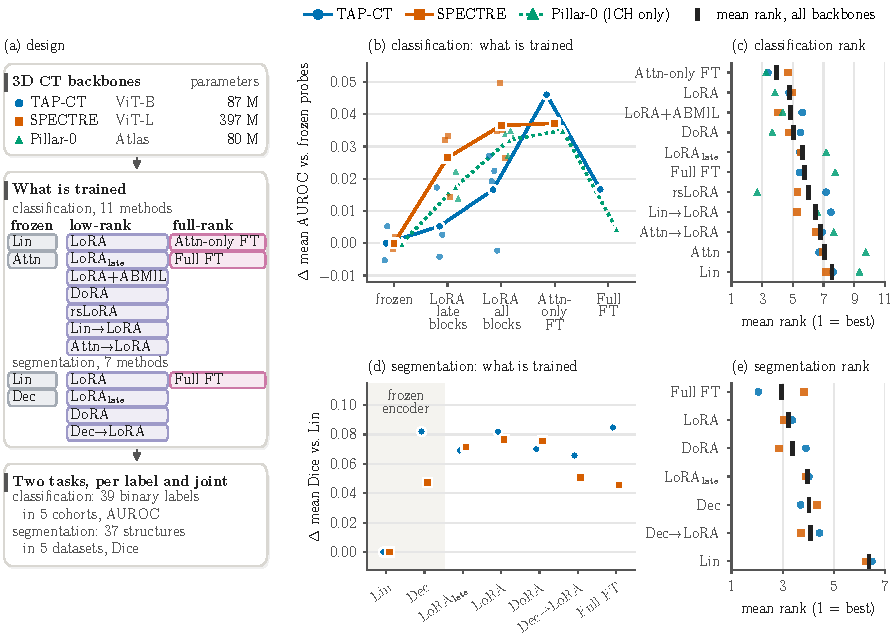
\includegraphics[width=\textwidth]{figures/fig_overview.pdf}
\vspace{-8pt}
\caption{Overview of the study. (a) Backbones, adaptation methods grouped by what they train, and tasks; Lin and Attn denote the linear and attentive probes and Dec the multi-depth decoder, all on the frozen encoder, and FT fine-tuning (Section~\ref{sec:ladder}). (b) Change in pooled held-out AUROC relative to the mean of each backbone's two frozen probes, where small markers denote methods (late blocks: LoRA$_{\text{late}}$ and the two-stage methods; all blocks: LoRA, LoRA+ABMIL, DoRA and rsLoRA) and lines group means. (c) Mean classification rank per backbone (markers) and pooled over backbones (bars). (d) Mean held-out Dice per segmentation method, computed on each backbone's own grid, where shading marks a frozen encoder. (e) Mean segmentation rank, as in (c). SPECTRE Full FT, which did not train, is excluded from (b) and (c); ranks are defined in Appendix~\ref{app:stats}.}
\label{fig:overview}
\end{figure}

A cohort collected for trauma or hemorrhage carries several findings per scan, and a segmentation dataset delineates several organs or lesions. Several pretrained 3D CT encoders are now public, among them TAP-CT \citep{veenboer2025tapct}, SPECTRE \citep{claessens2025spectre}, Pillar-0 \citep{agrawal2025pillar0}, CT-FM \citep{pai2025ctfm}, Merlin \citep{blankemeier2026merlin}, CT-CLIP \citep{hamamci2026ctrate} and FM-HCT \citep{zhu2025fmct}. Their evaluations mostly rank frozen representations with a linear, attentive or nearest-neighbor head \citep{veenboer2025tapct,claessens2025spectre}, and only some report end-to-end fine-tuning alongside \citep{pai2025ctfm,zhu2025fmct}. For natural images, comparisons on the same pretrained models showed that a frozen evaluation can be misleading. The linear-probe and fine-tuning accuracies of masked autoencoders were largely uncorrelated, and tuning a single transformer block raised ImageNet accuracy from 73.5\% to 81.0\% \citep{he2022mae}. Similarly, prompt tuning with under 1\% of the parameters outperformed full fine-tuning on 20 of 24 tasks \citep{jia2022vpt}, and full fine-tuning outperformed linear probing in distribution but not under distribution shift \citep{kumar2022lpft}. For 3D medical images such as CT, comparisons of this kind are few. Nonetheless, a group that adapts an encoder to a multi-label cohort or a multi-structure dataset, often with a few hundred to a few thousand labeled scans, has to decide whether to keep the encoder frozen, adapt it with low-rank adaptation (LoRA; \citealp{hu2022lora}) or fine-tune part or all of it, whether to train one model per label or one model for all labels of the dataset, and, for segmentation, which head turns the encoder tokens into a voxel map. A frozen probe answers none of these questions.

In medical imaging, the evidence for these choices comes mostly from 2D backbones and single tasks. On 2D medical classification, LoRA matches or surpasses full fine-tuning \citep{dutt2024peft,zhu2024melo}, and probing and fine-tuning of DINOv2 \citep{oquab2023dinov2} have been compared on radiology tasks \citep{baharoon2023dinov2med}. For 3D classification, \citet{liu2025anymc3d} found that frozen probing understates 2D and 3D foundation models, and that on the spleen-injury label of RSNA23 trauma, one of our labels, full fine-tuning of a convolutional and a Swin 3D model outperformed LoRA. Otherwise, parameter-efficient adaptation of 3D medical encoders has mostly been studied for segmentation, with adapters that lift the 2D Segment Anything model \citep{kirillov2023sam} to volumes \citep{gong20243dsamadapter,chen2024masam,wu2025medsa}, prompt tuning of a 3D U-Net \citep{fischer2024prompttuning}, and LoRA, adapters and full fine-tuning in few-shot transfer \citep{silvarodriguez2025fseft,ly2026seapeft}. For a 3D CT vision--language model, full and parameter-efficient fine-tuning performed similarly on one classification task \citep{kartika2026hcc}. However, each of these studies uses one backbone and one task, and none includes LoRA variants \citep{liu2024dora,kalajdzievski2023rslora}, probing before fine-tuning \citep{kumar2022lpft} or attention-only fine-tuning \citep{touvron2022three}. Joint training on many labels can help \citep{kim2023ctan} or hurt through conflicting gradients \citep{yu2020pcgrad,zhao2023mtlreview}. Yet joint and per-task adaptation of a 3D encoder have not been compared on the same labels \citep{veenboer2025tapct,liu2025anymc3d}. Our work aims to fill this gap.

To that end, we compared adaptation methods on five multi-label classification cohorts and five multi-structure segmentation datasets, under one protocol and on three encoders: two plain vision transformers (TAP-CT, SPECTRE) and the multi-scale transformer of Pillar-0 with its convolutional stem (Figures~\ref{fig:overview} and~\ref{fig:pipeline}). Classification was evaluated on all three encoders, with Pillar-0 on the head-CT cohort only and SPECTRE on the other four cohorts, and segmentation on TAP-CT and SPECTRE; every method was trained both per task and jointly. Our contributions can be summarized as follows:
\begin{itemize}\setlength{\itemsep}{1pt}
  \item We present a controlled comparison of \numClsMethodsN{} classification and \numSegMethodsN{} segmentation adaptation methods, ranging from frozen probes to low-rank adapters and full fine-tuning, on three 3D CT encoders from two architectural families, each trained per task and jointly (\numRunsMainN{} runs, plus \numRunsRevisionAllN{} repeats and controls).
  \item We find that, in classification, adapting the encoder's attention weights with LoRA outperforms both frozen probes on every encoder, whereas in segmentation a multi-depth decoder on the frozen encoder accounts for most of the gain, with LoRA beneath it changing Dice little on average.
  \item We find that one joint model per dataset performs on par with per-label models on average in classification but loses Dice in segmentation at our training budgets.
  \item We condense these findings into practical guidelines (Section~\ref{sec:guide}) and release our code, data splits and per-case predictions (\url{https://github.com/georgeyiasemis/beyond_frozen_encoders}).
\end{itemize}


\section{Methods}
\label{sec:methods}
\begin{figure}[t]
\centering
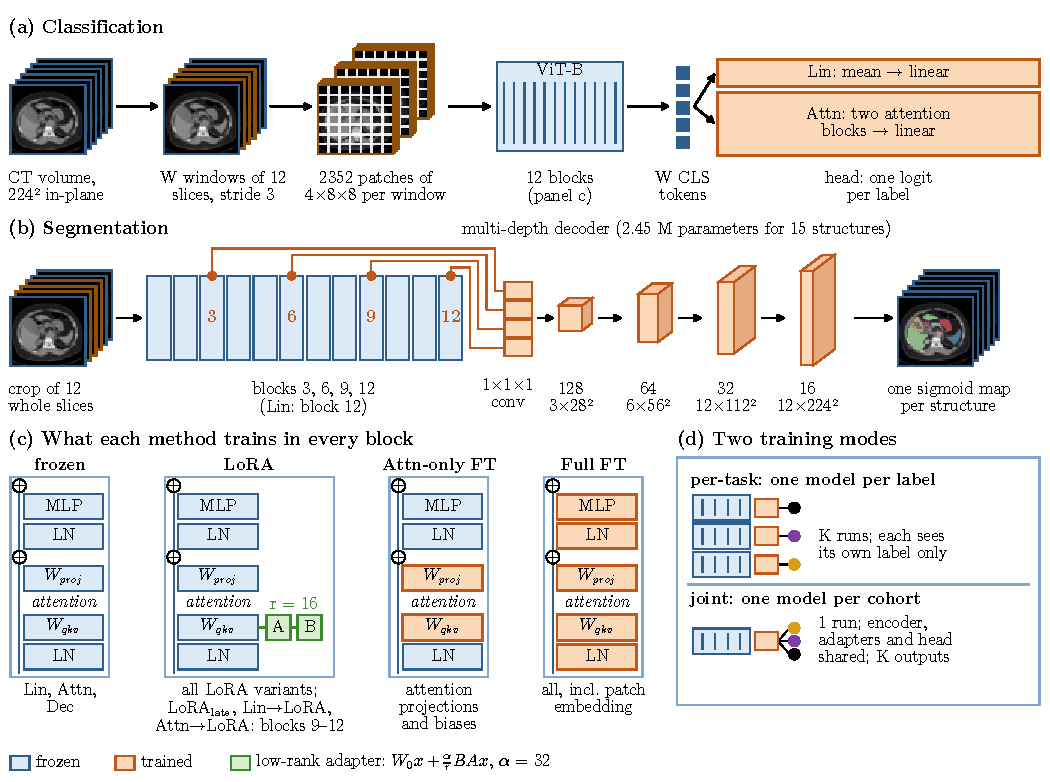
\includegraphics[width=\textwidth]{figures/fig_pipeline.pdf}
\vspace{-12pt}
\caption{How each task is run, shown for TAP-CT (other backbones: Figs.~\ref{fig:arms} and~\ref{fig:armsseg}, Appendix~\ref{app:details}). (a) Classification: the volume is split into $W$ 12-slice windows starting every 3 slices ($4\times8\times8$ patches), and the CLS token of every window enters the head, a linear layer on their mean (Lin) or an attentive probe (Attn), with one logit per label. (b) Segmentation: the tokens of blocks 3, 6, 9 and 12 feed a multi-depth decoder (2.45\,M parameters for 15 structures) with one sigmoid map per structure; Lin uses block 12 only. (c) Parameters each method trains in every encoder block; the head is always trained. (d) Per-task and joint training; in segmentation, a label is a structure and a cohort a dataset, and the 15-structure joint models train for three times the steps.}
\label{fig:pipeline}
\vspace{-5pt}
\end{figure}

\paragraph{Backbones.}\label{sec:backbones} First, \textbf{TAP-CT-B-3D} \citep{veenboer2025tapct} is a 12-block vision transformer pretrained using the DINOv2-style self-supervision on in-house CT (ViT-B; \citealp{dosovitskiy2021vit}), with $4\times8\times8$ voxel patches, a class (CLS) token, and four register tokens \citep{darcet2024registers}, applied to windows of $12\times224\times224$ voxels at native slice spacing (Fig.~\ref{fig:pipeline}). Second, \textbf{SPECTRE-Large} \citep{claessens2025spectre} is a 24-block ViT-L pretrained using self-distillation and vision-language alignment with radiology reports, with $16\times16\times8$ patches on $128\times128\times64$ crops, where for classification, 64 crops of a $512\times512\times256$ volume at $0.5\times0.5\times1$\,mm are summarized by its pretrained 4-block feature combiner. Third, Pillar-0 \citep{agrawal2025pillar0} is pretrained on CT and breast magnetic resonance imaging (MRI) data from a single academic center. We use its head-CT Atlas encoder, which comprises a convolutional stem followed by three stages of multi-scale window-attention blocks operating over the whole volume; given its head-CT specialization, we evaluate it only on RSNA19 ICH. Inputs follow each model's own orientation, spacing, and intensity normalization (Fig.~\ref{fig:arms} and Appendix~\ref{app:details}). We are among the authors of TAP-CT.

\paragraph{Classification Methods.}\label{sec:ladder} The methods differ only in which weights of each encoder block they train, among its attention, feed-forward (MLP) and layer-normalization (LN) weights (Figs.~\ref{fig:pipeline}c and~\ref{fig:arms}c). We analyze two \textit{types of probes} on the frozen features: \textbf{Lin}, a linear layer on a pooled feature, and \textbf{Attn}, an attentive probe \citep{bardes2024vjepa,chen2024cae} in which a learnable CLS token joins the window, crop or scale tokens and two self-attention blocks run over the set. We also test different \emph{low-rank adapters} on the query/key/value projections together with the attentive probe: \textbf{LoRA}, rank 16 ($\alpha=32$) on every block \citep{hu2022lora}; \textbf{LoRA$_{\text{late}}$}, on the last third of the blocks (for Pillar-0, its last stage, i.e., 8 of 12 blocks); \textbf{LoRA+ABMIL}, with tokens first pooled by gated attention-based multiple-instance learning (ABMIL; \citealp{ilse2018abmil}); \textbf{DoRA}, weight-decomposed LoRA \citep{liu2024dora}; and \textbf{rsLoRA}, rank-stabilized LoRA \citep{kalajdzievski2023rslora}, whose $\alpha/\sqrt{r}$ scaling is four times the LoRA scale at $r=16$. We also test \emph{two-stage schedules}: \textbf{Lin$\to$LoRA} and \textbf{Attn$\to$LoRA}, which train the probe for half the budget and then add late-block LoRA, keeping the probe's head \citep{kumar2022lpft}. Finally, for the \emph{full-rank fine-tuning (FT)} we have \textbf{Attn-only FT} which trains every parameter of the attention modules \citep{touvron2022three} and \textbf{Full FT} which trains every parameter of the encoder, together with the attentive head.

\paragraph{Segmentation Methods.}\label{sec:segmethods} For the segmentation tasks, we use the TAP-CT and SPECTRE backbones. We test two segmentation heads: \textbf{Lin}, which is a $1\times1\times1$ convolution on the deepest token grid, upsampled trilinearly, and \textbf{Dec} which is a light multi-depth decoder similar to UNETR \citep{hatamizadeh2022unetr} but without its skip connections from the input: the token grids of four depths are projected, concatenated, fused and upsampled to the voxel grid by $3^3$ convolutions (Figs.~\ref{fig:pipeline}b and~\ref{fig:armsseg}). \textbf{LoRA}, \textbf{LoRA$_{\text{late}}$} and \textbf{DoRA} add the adapters of classification under the multi-depth decoder, \textbf{Full FT} trains the encoder with it, and \textbf{Dec$\to$LoRA} trains Dec for half the budget before adding all-block LoRA. Predictions are independent sigmoid functions per structure.

\paragraph{Per-task and Joint Training.} Every cohort and dataset is trained in two modes with identical data and selection (Fig.~\ref{fig:pipeline}d): \emph{per-task}, where we have one model per label, and \emph{joint}, where we use one model with shared encoder, adapters and head and one output per label or structure. In this setup, we define a \emph{label-mode pair} as one label on one backbone in one of the two modes. Moreover, a per-task model has one output, whereas a joint model has one output per label or structure and sums the classification loss over the labels annotated for a case and it averages the segmentation loss over structures (Equations~\ref{eq:lcls} and~\ref{eq:lseg}, Appendix~\ref{app:details}).


\section{Experiments}
\label{sec:setup}
\paragraph{Data.} Classification uses five public CT cohorts with \numLabelsN{} binary labels (Tabs.~\ref{tab:cohorts} and~\ref{tab:labelcounts} and Fig.~\ref{fig:examples} in Appendix~\ref{app:cohorts}). The CVPR26 cohort is the release of the CVPR 2026 3D CT foundation-model challenge, which contains AMOS \citep{ji2022amos} with 15 disease labels, COVID-CTset \citep{rahimzadeh2021covidctset} and LUNA25 nodule malignancy \citep{peeters2026luna25}. FDG-PET/CT \citep{gatidis2022fdgpetct} provides four diagnosis groups, which we predict from the CT alone. The remaining cohorts are RSNA 2022 cervical-spine fracture detection (RSNA22 C-spine; \citealp{lin2023rsnacsfdata}), RSNA 2023 abdominal trauma detection (RSNA23 trauma; \citealp{rudie2024ratic}) and RSNA 2019 intracranial hemorrhage (ICH) detection (RSNA19 ICH; \citealp{flanders2020rsnaich}). Segmentation uses AMOS22 (15 organs; \citealp{ji2022amos}), KiTS23 \citep{heller2023kits21}, LiTS \citep{bilic2023lits}, MSD Pancreas \citep{antonelli2022msd} and TotalSegmentator \citep{wasserthal2023totalsegmentator,wasserthal2026totalsegdata}, whose 117 structures we merge into 15 (Tab.~\ref{tab:totalseg}), for \numStructuresN{} structures in total. For the CVPR26 cohort and AMOS22, the official validation cases are divided into a selection and a held-out half, whereas the other sources use fixed seeded splits of the released labeled cases, and TotalSegmentator holds out its official test split.

\paragraph{Optimization.} All runs use AdamW with a 10\% linear warm-up, cosine decay to $10^{-6}$ and bf16 precision. A classification run trains for 8000 steps at batch size 1 on a masked, positive-weighted binary cross-entropy, and a segmentation run trains for 8000 steps of four crops on the sum of soft Dice and binary cross-entropy. For the two-stage methods, we split the budget in halves. Consequently, a joint model uses $1/K$ of the steps of the $K$ per-task models it replaces, except for the 15-structure joint segmentation models (AMOS22, TotalSegmentator), which train for 24\,000 steps. Each method has one default learning rate, set by what it trains: $10^{-3}$ for the classification linear probe and the segmentation decoder, $10^{-2}$ for the segmentation linear probe, $10^{-4}$ for the attentive probe and the adapters, and $2\times10^{-5}$ for encoder weights. None of these settings was tuned on our data (Tabs.~\ref{tab:optim} and~\ref{tab:optimseg}). Every 1000 steps, the model is evaluated on the selection split, and the checkpoint with the best macro AUROC or mean Dice is kept and its held-out metric reported.

\paragraph{Evaluation.} We report AUROC per label and Dice per structure and case, on each backbone's working grid \citep{maierhein2024metrics}. Methods are compared per label-mode pair with DeLong's test \citep{delong1988} for AUROC or a paired case bootstrap for Dice, both with Benjamini-Hochberg correction \citep{benjamini1995fdr}, and are ranked within each pair that has every method. TotalSegmentator per-structure models were trained for Lin, Dec, LoRA and Full FT only. The main comparisons are summarized at label level, where each label counts once with its two modes averaged, with 95\% intervals from a bootstrap over cohorts, labels and held-out cases (Appendix~\ref{app:stats}). As the bootstrap draws only four or five cohorts per backbone, which makes its intervals optimistic, and does not include the variation between training seeds, we also count the cohorts with a positive mean difference. We flag a method as not trained when the median standard deviation of its held-out probabilities is below \numSpreadMinValue{} (Appendix~\ref{app:stats}). Only SPECTRE Full FT was flagged (\numSpreadSpectreFullft{}, against at least \numSpreadOthermin{} for every other method). We report it in the tables but exclude it from ranks and from averages over methods. The joint models of Lin, LoRA, Attn-only FT and Full FT (classification) and of Dec, LoRA and Full FT (segmentation) were trained with two further seeds (Appendix~\ref{app:revision}).


\section{Results}
\label{sec:results}
\begin{table}[tb]
\centering
\caption{Main comparisons between methods per backbone. Each entry is the held-out AUROC (classification) or Dice (segmentation) of the first method minus that of the second, averaged over labels or structures, with the 95\% bootstrap interval over cohorts, labels and cases in brackets, which does not include seed variation (Appendix~\ref{app:stats}). The $>0$ columns count the cohorts (datasets) with a positive mean difference. Lin and Attn denote the frozen linear and attentive probes and Dec the frozen multi-depth decoder; Joint $-$ per-task compares one model per cohort with one model per label and averages over methods. Each label's per-task and joint values are averaged, except in the two LoRA $-$ Dec sub-rows. Pooled estimates are in Table~\ref{tab:cis}. $^\dagger$Includes runs that did not train (Section~\ref{sec:setup}).}
\label{tab:key}
\vspace{-6pt}
\renewcommand{\mci}[3]{#1\,{\scriptsize[#2, #3]}}\adjustbox{max width=\textwidth}{\small\setlength{\tabcolsep}{3.5pt}
\begin{tabular}{@{}lcccccc@{\hspace{10pt}}lcccc@{}}
\toprule
\multicolumn{7}{c}{\textit{Classification} (AUROC)} & \multicolumn{5}{c}{\textit{Segmentation} (Dice)} \\
\cmidrule(r){1-7}\cmidrule(l){8-12}
 & \multicolumn{2}{c}{TAP-CT} & \multicolumn{2}{c}{SPECTRE} & \multicolumn{2}{c}{Pillar-0} & & \multicolumn{2}{c}{TAP-CT} & \multicolumn{2}{c}{SPECTRE} \\
\cmidrule(lr){2-3}\cmidrule(lr){4-5}\cmidrule(lr){6-7}\cmidrule(lr){9-10}\cmidrule(lr){11-12}
Comparison & Mean & $>0$ & Mean & $>0$ & Mean & $>0$ & Comparison & Mean & $>0$ & Mean & $>0$ \\
\midrule
LoRA $-$ Lin & \mci{$+0.032$}{$+0.007$}{$+0.053$} & 4/5 & \mci{$+0.037$}{$+0.009$}{$+0.075$} & 4/4 & \mci{$+0.033$}{$+0.021$}{$+0.044$} & 1/1 & Dec $-$ Lin & \mci{$+0.085$}{$+0.055$}{$+0.109$} & 5/5 & \mci{$+0.061$}{$+0.027$}{$+0.088$} & 5/5 \\
LoRA $-$ Attn & \mci{$+0.022$}{$+0.006$}{$+0.042$} & 5/5 & \mci{$+0.033$}{$+0.003$}{$+0.078$} & 4/4 & \mci{$+0.034$}{$+0.021$}{$+0.052$} & 1/1 & LoRA $-$ Dec & \mci{$-0.005$}{$-0.021$}{$+0.024$} & 4/5 & \mci{$+0.023$}{$-0.018$}{$+0.076$} & 4/5 \\
Attn-only FT $-$ LoRA & \mci{$+0.019$}{$-0.001$}{$+0.054$} & 4/5 & \mci{$+0.002$}{$-0.037$}{$+0.026$} & 2/4 & \mci{$+0.001$}{$-0.002$}{$+0.004$} & 1/1 & \quad per-structure & \mci{$-0.021$}{$-0.036$}{$+0.002$} & 2/5 & \mci{$+0.006$}{$-0.003$}{$+0.031$} & 5/5 \\
Full FT $-$ Lin & \mci{$+0.022$}{$-0.061$}{$+0.068$} & 4/5 & \mci{$-0.117^{\dagger}$}{$-0.195$}{$-0.059$} & 0/4 & \mci{$+0.004$}{$-0.013$}{$+0.021$} & 1/1 & \quad joint & \mci{$+0.011$}{$-0.021$}{$+0.066$} & 4/5 & \mci{$+0.040$}{$-0.039$}{$+0.147$} & 4/5 \\
 &  &  &  &  &  &  & Full FT $-$ Dec & \mci{$0.000$}{$-0.024$}{$+0.016$} & 4/5 & \mci{$-0.003$}{$-0.035$}{$+0.009$} & 2/5 \\
\cmidrule(r){1-7}\cmidrule(l){8-12}
Joint $-$ per-task & \mci{$+0.012$}{$-0.014$}{$+0.038$} & 3/5 & \mci{$-0.003$}{$-0.044$}{$+0.051$} & 3/4 & \mci{$-0.008$}{$-0.013$}{$-0.001$} & 0/1 & Joint $-$ per-task & \mci{$-0.046$}{$-0.090$}{$-0.008$} & 0/5 & \mci{$-0.058$}{$-0.093$}{$-0.009$} & 0/5 \\
\bottomrule
\end{tabular}
}
\end{table}

Table~\ref{tab:key} summarizes the main comparisons; per-label results, paired tests, seed repeats and controls, and success and failure cases are given in Appendices~\ref{app:perlabel}, \ref{app:paired}, \ref{app:revision} and~\ref{app:cases}.

\subsection{Classification}
\label{sec:clsres}

\begin{figure}[tb]
\centering
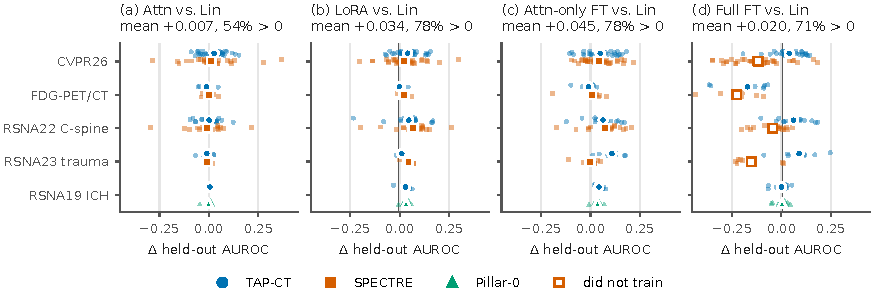
\includegraphics[width=\textwidth]{figures/fig_cls.pdf}
\vspace{-8pt}
\caption{Per-label change in held-out AUROC relative to the linear probe of the same backbone, cohort and training mode, for (a) the frozen attentive probe, (b) LoRA and (c) attention-only fine-tuning. Small markers denote individual label--mode pairs and large markers the mean per cohort. Panel titles give the mean change and the share of pairs above zero over all backbones. All methods, including full fine-tuning, are shown in Figure~\ref{fig:methods}.}
\label{fig:cls}
\end{figure}

\begin{figure}[tb]
\centering
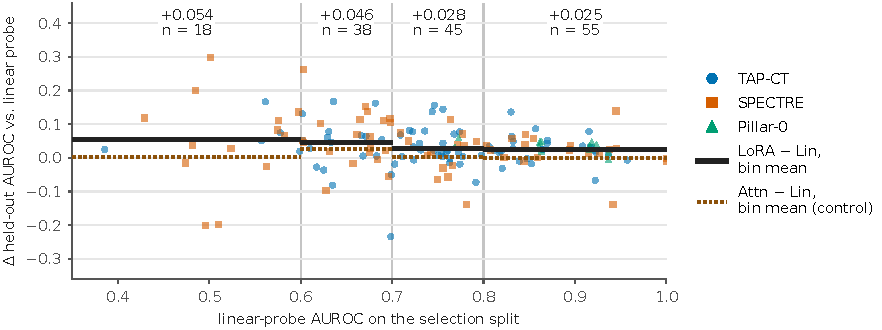
\includegraphics[width=\textwidth]{figures/fig_gain_vs_probe.pdf}
\vspace{-8pt}
\caption{Gain of LoRA over the linear probe in held-out AUROC, per label--mode pair, against the linear probe's selection-split AUROC (marker shape: backbone). Horizontal segments give bin means over all backbones, with bin edges at 0.6, 0.7 and 0.8. The dotted segments show the same bin means for the frozen attentive probe, as a negative control. Above each bin, the LoRA mean, the attentive-probe mean (brown) and the number of pairs are printed.}
\label{fig:gainprobe}
\end{figure}

Across TAP-CT, SPECTRE and Pillar-0, adapting the encoder with LoRA improved held-out AUROC over both frozen probes, by \magn{\numCiClsloralinAllMeandiff} over the linear probe and by \magn{\numCiClsloraattnAllMeandiff} over the frozen attentive probe, which uses the same head (Table~\ref{tab:cis}; per backbone in Table~\ref{tab:key} and Figure~\ref{fig:cls}). Both 95\% intervals exclude zero, and the improvement over the attentive probe was positive in all \numCiClsloraattnAllClustersN{} cohort--backbone pairs. The mean held-out AUROC rose from \pooledtapctlin{} to \pooledtapctlora{} on TAP-CT, from \pooledspectrelin{} to \pooledspectrelora{} on SPECTRE and from \pooledpillarZlin{} to \pooledpillarZlora{} on Pillar-0 (Table~\ref{tab:headline}). Fine-tuning all parameters of the attention modules showed the same pattern, with gains of \magn{\numCiClsattnftlinAllMeandiff} and \magn{\numCiClsattnftattnAllMeandiff}, respectively (Table~\ref{tab:cis}). In contrast, the frozen attentive probe improved on the linear probe by only \magn{\numCiClsattnlinAllMeandiff}, which suggests that the gain stems from adapting the encoder rather than from the head. As shown in Figure~\ref{fig:gainprobe}, the gain was largest for labels on which the linear probe performed worst (\magn{\numGainbinLowMeandiff} at a selection AUROC of at most 0.6, against \magn{\numGainbinTopMeandiff} above 0.8). Moreover, the gain persisted after excluding FDG-PET/CT and COVID-CTset, whose labels may be predictable from the acquisition rather than the anatomy (\magn{\numCiClsloralinnoscAllMeandiff}; Table~\ref{tab:cis}). LoRA also outperformed the linear probe in \numSeedsclsLoraLinAllPosN{} of \numSeedsclsLoraLinAllPairsN{} cohort--seed pairs of the repeated joint models (Table~\ref{tab:seedscls}).

At the default settings, fine-tuning all attention parameters achieved the best mean rank over all label--mode pairs (\numRankAttnftMean{}, against \numRankLoraMean{} for LoRA; Figure~\ref{fig:overview}c) and ranked above LoRA on every backbone. It outperformed LoRA in \numSeedsclsAttnftLoraAllPosN{} of \numSeedsclsAttnftLoraAllPairsN{} cohort--seed pairs of the repeated joint models and by \magn{\numCiClsattnftloraAllMeandiff} on average over the main runs, although this interval includes zero (Table~\ref{tab:cis}); the difference was largest on TAP-CT (\magn{\numCiClsattnftloraTapctMeandiff}). LoRA updates \numParamsratioPillarZAttnftLora{} to \numParamsratioSpectreAttnftLora{} times fewer encoder parameters (Figure~\ref{fig:arms}c), yet this did not make training cheaper. Its peak GPU memory per step was within \numCostClsLoraAttnftMaxGibdiff{}\,GiB of that of attention-only fine-tuning on every backbone and its steps were not faster (Table~\ref{tab:cost}), so the saving lies in the encoder weights stored per model. Fine-tuning the MLP weights instead of the attention weights performed on par with attention-only fine-tuning on TAP-CT and Pillar-0, but remained behind it by \magn{\numCtrlSpectreMlpftAttnftMeandiff} on SPECTRE (joint models; Table~\ref{tab:controls}).

Full fine-tuning required its own setting. With the default setting, it was ahead of the linear probe on TAP-CT by \magn{\numCiClsfullftlinTapctMeandiff} on average, with an interval that includes zero (Table~\ref{tab:key}), and was the best joint model on RSNA23 trauma (Table~\ref{tab:cls}), where \citet{liu2025anymc3d} also found full fine-tuning ahead of LoRA for spleen injury. On Pillar-0 it performed on par with the linear probe, whereas on SPECTRE it did not train: its median selection AUROC remained at \numTrajSpectrefullftLast{}, against \numTrajSpectreattnftLast{} for attention-only fine-tuning at the same learning rates (Figure~\ref{fig:fullftspectre}). With layer-wise learning-rate decay of 0.75 per block, the best of three alternative settings on selection data, SPECTRE Full FT trained and was ahead of LoRA by \magn{\numFixselSpectreLoraMeandiff} in the joint models (Table~\ref{tab:fullftfix}). However, this comparison favors full fine-tuning, as LoRA was not re-tuned.

On average over backbones, none of the LoRA variants improved on plain LoRA by more than \magn{\numVsloraAllBabmilMeandiff} (Figure~\ref{fig:methods}). The two-stage schedules and rsLoRA were behind LoRA by \magn{\numVsloraAllLinThenLoragMeandiff} to \magn{\numVsloraAllAttnThenLoragMeandiff}. At a quarter of the learning rate, which matches its update scale to that of LoRA, rsLoRA performed on par with LoRA on SPECTRE and Pillar-0 but remained behind it on TAP-CT by \magn{\numCtrlTapctRsloraLowlrLoraMeandiff} (Table~\ref{tab:controls}). These rankings hold for one default setting and 8000 steps per method. On CVPR26, a 26\,000-step schedule changed the joint models by $\numJointlongTapctMindiff$ to $\numJointlongTapctMaxdiff$ on TAP-CT and by $\numJointlongSpectreMindiff$ to $\numJointlongSpectreMaxdiff$ on SPECTRE, depending on the method (Table~\ref{tab:ladder}), which is as large as the differences between methods.

\subsection{Segmentation}
\label{sec:segres}

Replacing the linear probe by the frozen multi-depth decoder improved Dice on every dataset and backbone, by \magn{\numSegdeltaTapctLinDecMeandiff} on TAP-CT and \magn{\numSegdeltaSpectreLinDecMeandiff} on SPECTRE (Table~\ref{tab:key}; examples in Figure~\ref{fig:examplesseg}, Appendix~\ref{app:cases}). On TAP-CT, this accounted for all of the gain of LoRA over the linear probe (\magn{\numSegdeltaTapctLinLoraMeandiff}), and on SPECTRE for most of it (\magn{\numSegdeltaSpectreLinLoraMeandiff}). The pretrained weights nonetheless mattered, as the TAP-CT architecture trained from a random initialization was behind fine-tuning of the pretrained encoder at the same budget on every dataset, by \magn{\numScratchLitsTapctMeandiff} to \magn{\numScratchTotalsegTapctMeandiff} Dice (Table~\ref{tab:scratch}).

On top of the decoder, adapting the encoder changed Dice little on average. LoRA changed Dice relative to the frozen decoder by $\numCiSegloradecTapctMeandiff$ on TAP-CT and $\numCiSegloradecSpectreMeandiff$ on SPECTRE, with intervals that include zero (Table~\ref{tab:key}, Figure~\ref{fig:key}; per-structure changes in Figure~\ref{fig:seg}, Appendix~\ref{app:paired}). Its largest gain occurred where the frozen decoder was weakest, in the SPECTRE AMOS22 joint model (\numSegAmosBBSpectreJointDec{} to \numSegAmosBBSpectreJointLora{}; Table~\ref{tab:segbudget}). Full fine-tuning achieved the best mean rank (\numSegrankFullftMean{}, against \numSegrankLoraMean{} for LoRA; Figure~\ref{fig:overview}e), driven by its rank on TAP-CT (\numSegrankTapctFullftMean{}). However, its mean change on TAP-CT was $\numSegdeltaTapctDecFullftMeandiff$, because \numSegdeltaTapctDecFullftDropN{} structure--mode pairs lost more than 0.1, among them the AMOS22 esophagus of the joint model ($\numSegdeltaTapctDecFullftMindiff$; Appendix~\ref{app:cases}). In addition, tripling the steps of the 15-structure joint models improved their Dice by \magn{\numSegbudgetgainTapctMeandiff} on TAP-CT and \magn{\numSegbudgetgainSpectreMeandiff} on SPECTRE (Table~\ref{tab:segbudget}), and \numConvSegAllLateBetter\% of segmentation runs selected one of their last two validations (Figure~\ref{fig:segconv}). These comparisons therefore rank methods at a fixed budget rather than at convergence.

\begin{figure}[tb]
\centering
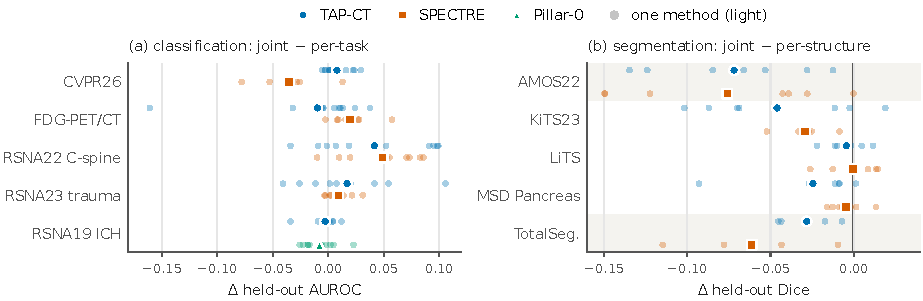
\includegraphics[width=\textwidth]{figures/fig_joint_main.pdf}
\vspace{-14pt}
\caption{Joint minus per-task training. (a) Joint minus per-task held-out AUROC per classification cohort and (b) joint minus per-structure held-out Dice per segmentation dataset. Large markers denote the mean over methods and labels (structures) per backbone, and light markers, in the backbone's color, individual methods. Shaded rows mark the 15-structure datasets, whose joint models were trained for 24\,000 steps. Values right of zero favor one joint model per dataset. Per-label values are given in Appendix~\ref{app:perlabel} and Figure~\ref{fig:joint}.}
\label{fig:jointmain}
\end{figure}

\subsection{Per-task and Joint Training}
\label{sec:jointres}

In classification, one joint model per cohort performed on par with one model per label on average, at a fraction of the training. Joint minus per-task AUROC was $\numCiClsjointAllMeandiff$ over TAP-CT, SPECTRE and Pillar-0 (interval $\numCiClsjointAllLodiff$ to $\numCiClsjointAllHidiff$; Table~\ref{tab:cis}), whereas a joint model uses $1/K$ of the training steps of the $K$ per-label models it replaces. On Pillar-0 alone, the joint models were slightly behind ($\numCiClsjointPillarZMeandiff$, interval $\numCiClsjointPillarZLodiff$ to $\numCiClsjointPillarZHidiff$). Per cohort and averaged over methods, the difference ranged from $\numJointdeltaMin$ to $\numJointdeltaMax$ (Figure~\ref{fig:jointmain}a; per method in Figure~\ref{fig:joint}).

\label{sec:jointseg}In segmentation, in contrast, the joint models lost Dice, mostly on small structures and partly through the smaller budget per structure. With each structure counted once (Table~\ref{tab:key}), one joint model per dataset changed Dice by $\numCiSegjointTapctMeandiff$ on TAP-CT and $\numCiSegjointSpectreMeandiff$ on SPECTRE, most on the 15-structure AMOS22 (Figure~\ref{fig:jointmain}b). Averaged over structure--method pairs, the joint model lost \magn{\numSegjointTapctMeandiff} Dice on TAP-CT and \magn{\numSegjointSpectreMeandiff} on SPECTRE. Much of this loss came from \numSegcollapseN{} of \numSegcollapseCellsN{} pairs on small structures, namely the adrenal glands and esophagus of AMOS22 and the merged glands of TotalSegmentator, on which the joint model scored below 0.01. Excluding these pairs, the losses were \magn{\numSegjointTapctNocollapseMeandiff} and \magn{\numSegjointSpectreNocollapseMeandiff}, respectively. Training crops are centered on a random foreground voxel of all structures together, so small structures rarely lie at the center of a crop; we did not test structure-balanced sampling \citep{isensee2021nnunet}. At matched total compute, with each per-structure model trained for 1600 steps, the joint frozen decoder and joint full fine-tuning remained behind per-structure models in three of the four pairs (Table~\ref{tab:segcm}). The joint LoRA model, in contrast, outperformed per-structure LoRA by \magn{\numCmTotalsegSpectreLoraJointdiff} to \magn{\numCmAmosBBSpectreLoraJointdiff} Dice, but per-structure LoRA at 1600 steps reached only \numCmAmosBBTapctLoraMatchedMean{} to \numCmTotalsegSpectreLoraMatchedMean{} Dice, against \numCmAmosBBSpectreDecMatchedMean{} to \numCmTotalsegSpectreDecMatchedMean{} for per-structure decoders. The smaller budget per structure therefore explains part, but not all, of the loss of the joint models.


\section{A practical guide and discussion}
\label{sec:discussion}\label{sec:guide}
Each step gives the setting we used and what it changed (Table~\ref{tab:key}), with every method at one default setting; Table~\ref{tab:cost} gives the training cost.
\begin{enumerate}\setlength{\itemsep}{1pt}
  \item \textbf{Classification: adapt the encoder's attention weights.} Rank-16 LoRA ($\alpha=32$, learning rate $10^{-4}$) on every block added $\numCiClsloralinAllMeandiff$ AUROC over the linear probe and $\numCiClsloraattnAllMeandiff$ over the attentive probe, positive in all \numCiClsloraattnAllClustersN{} cohort--backbone pairs. Fine-tuning the attention weights in full was ahead of LoRA in \numSeedsclsAttnftLoraAllPosN{} of \numSeedsclsAttnftLoraAllPairsN{} seed pairs, by $\numCiClsattnftloraAllMeandiff$ on average, at similar GPU memory and time per step; LoRA stores \numParamsratioPillarZAttnftLora{} to \numParamsratioSpectreAttnftLora{} times fewer weights per model. Fine-tuning the MLP weights instead was close on TAP-CT and Pillar-0 and behind on SPECTRE. With LoRA, use plain LoRA: no variant improved on it by more than $\numVsloraAllBabmilMeandiff$.
  \item \textbf{Classification: start with one model per cohort.} It was on average level with per-label models ($\numCiClsjointAllMeandiff$) at $1/K$ of the training, but per cohort the difference ranged from $\numJointdeltaMin$ to $\numJointdeltaMax$, so compare the two on selection data when the budget allows.
  \item \textbf{Segmentation: put a multi-depth decoder on the frozen encoder.} It added $\numSegdeltaTapctLinDecMeandiff$ (TAP-CT) and $\numSegdeltaSpectreLinDecMeandiff$ (SPECTRE) Dice over a linear probe, on every dataset. Adapting the encoder beneath it changed Dice by at most $\numSegdeltaSpectreDecDoraMeandiff$ on average (DoRA on SPECTRE); full fine-tuning ranked best but lost more than 0.1 Dice on some small structures, so check Dice per structure.
  \item \textbf{Segmentation: train one model per structure when the budget allows.} On both 15-structure datasets, per-structure models at 8000 steps were ahead of the joint model for the frozen decoder, LoRA and full fine-tuning, and at matched total compute per-structure decoders were still ahead of the joint decoder in three of four pairs. Otherwise check the Dice of small structures, where the joint models failed.
  \item \textbf{Full fine-tuning: lower the learning rate of early blocks.} With the encoder learning rate of the other methods it did not train on SPECTRE (near-constant predictions); layer-wise decay of 0.75 per block fixed it. Check that held-out predictions vary between cases.
\end{enumerate}

\paragraph{Limitations.} Each method has one untuned default setting, and only full fine-tuning was retrained after it failed, so the ranking among the stronger methods may change with tuning; seeds were repeated only for joint models. Per-label tests have little power: LoRA was significantly ahead of the linear probe on \numSigbysizeSmallSig\% of labels with fewer than 100 held-out cases and on \numSigbysizeLargeSig\% of those with 400 or more. Segmentation had not converged and is scored on each backbone's working grid, so it ranks adaptation methods rather than measuring the distance to nnU-Net \citep{isensee2021nnunet} or to models pretrained on segmentation labels \citep{li2024suprem,he2024vista3d}. SPECTRE saw AMOS, LUNA25, LiTS, MSD Pancreas and most held-out KiTS23 cases, without labels, in self-supervised pretraining (Table~\ref{tab:overlap}), which may favor it over the other backbones on these sets.


\clearpage
\bibliography{refs}

\appendix
% appendix pages are filled from the top; no stretching of the space between heading and floats
\raggedbottom
\section{Training and evaluation details}
\label{app:details}

\begin{figure}[H]
\centering
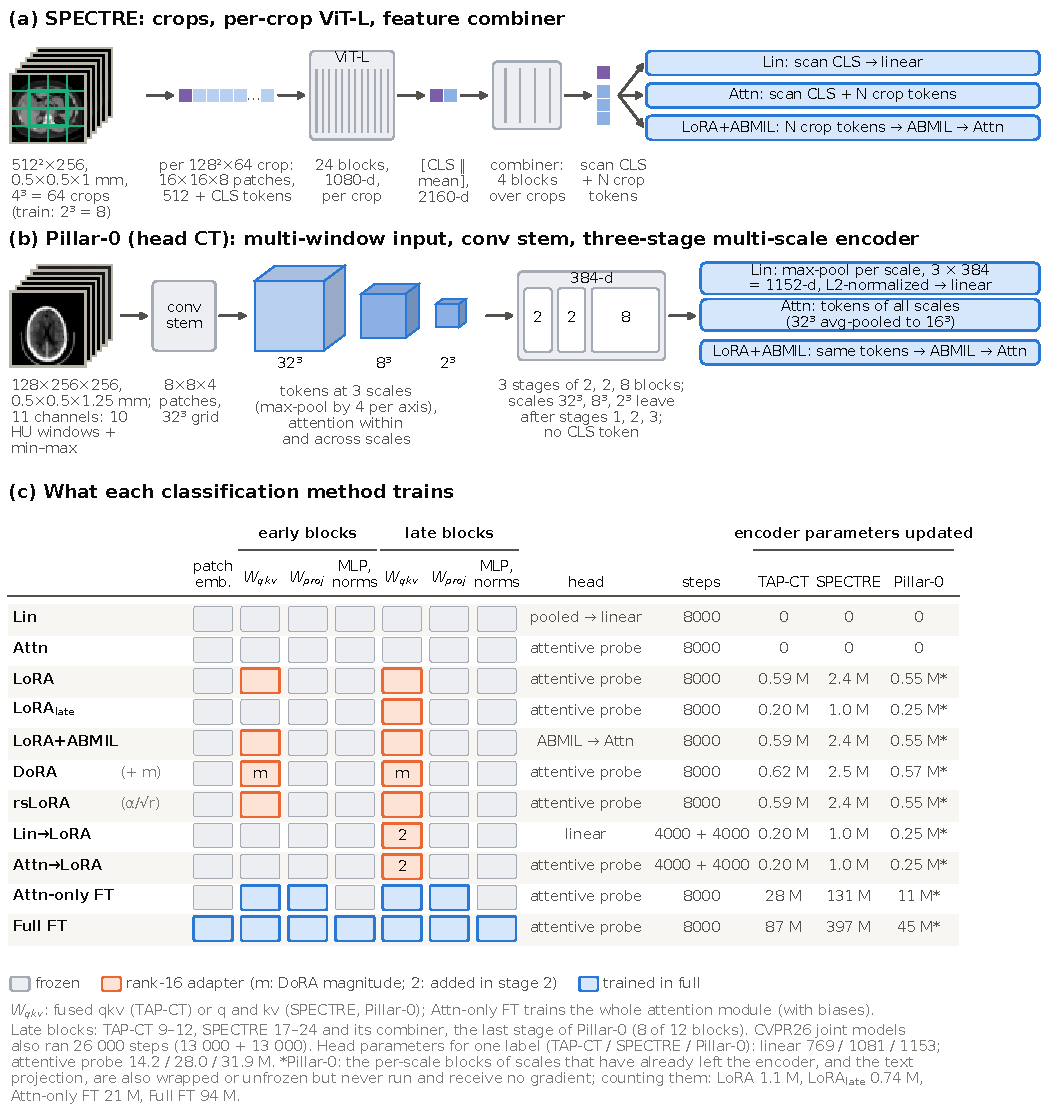
\includegraphics[width=0.88\textwidth,height=0.66\textheight,keepaspectratio]{figures/fig_arms.pdf}
\caption{Classification with SPECTRE and Pillar-0, drawn from the implementation (TAP-CT: Figure~\ref{fig:pipeline}). (a, b) How each backbone turns a volume into the tokens the heads read: SPECTRE encodes crops separately and summarizes them with its pretrained feature combiner; Pillar-0 encodes the whole head CT with a convolutional stem and a three-stage multi-scale transformer. (c) The encoder components each of the eleven methods trains, its head, its number of steps and the number of encoder parameters that receive a gradient; for Pillar-0 this excludes per-scale blocks that never run, and the note gives the logged counts that include them.}
\label{fig:arms}
\end{figure}

\begin{figure}[H]
\centering
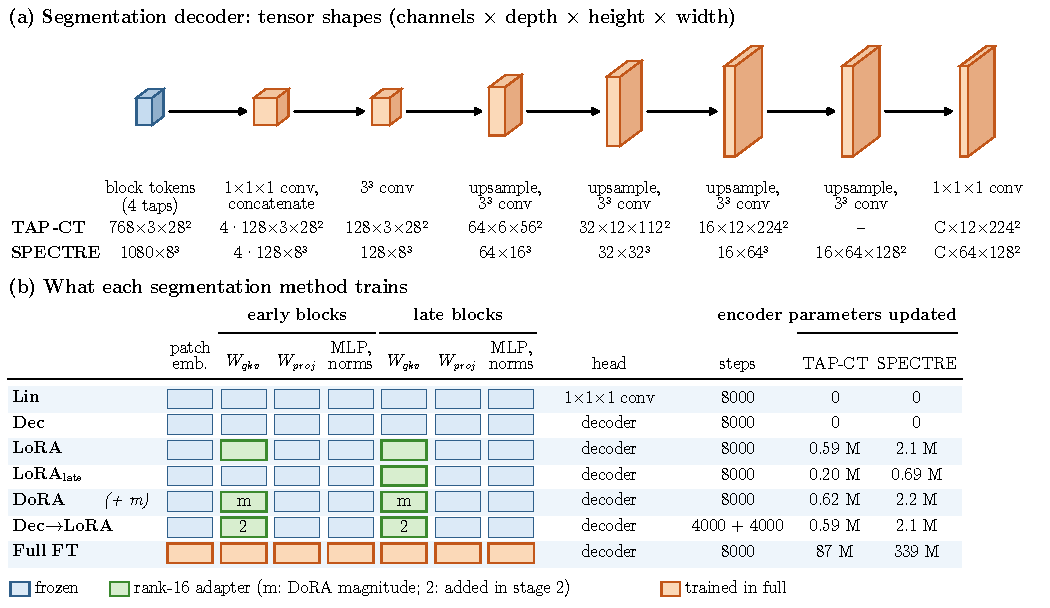
\includegraphics[width=\textwidth,height=0.74\textheight,keepaspectratio]{figures/fig_arms_seg.pdf}
\caption{Segmentation decoder and methods, drawn from the implementation. (a) Tensor shapes through the decoder for TAP-CT and SPECTRE, from the four encoder taps to the $C$ output maps (one per structure). (b) The encoder components each of the seven methods trains and the number of encoder parameters that receive a gradient; the SPECTRE counts exclude the feature combiner, which the adapters wrap but which does not enter the segmentation features.}
\label{fig:armsseg}
\end{figure}

\paragraph{Input preprocessing.} Every volume is reoriented to the frame of the backbone's pretraining and resampled to its grid. TAP-CT: LPS, native slice spacing, in-plane trilinear resize to $224\times224$, depth padded with air to at least 12 slices and to a multiple of 4; HU clipped to $[-1008, 822]$ and standardized with the model's mean and standard deviation; windows of 12 slices with a stride of 3 slices plus a final window ending at the last slice (at most 32 windows per training step, all windows at evaluation). SPECTRE: RAS, $0.5\times0.5\times1$\,mm, centered $512\times512\times256$ field of view padded with the scan minimum, HU in $[-1000, 1000]$ scaled to $[0,1]$; a $4\times4\times4$ grid of 64 crops of $128\times128\times64$ voxels at evaluation and a random contiguous $2\times2\times2$ sub-grid of 8 crops at training; each crop is summarized by its CLS token concatenated with its mean patch token before the feature combiner. Pillar-0: LPI, $0.5\times0.5\times1.25$\,mm, centered $128\times256\times256$ volume, eleven input channels (ten fixed center/width windows and a per-volume min--max channel), one forward pass; the linear head reads the model's L2-normalized pooled embedding (three scales concatenated, 1152-d), the attentive head reads the tokens of the three scales, any scale with more than 4096 tokens being average-pooled on its grid. For segmentation, TAP-CT keeps the classification grid (in-plane 224, native depth) and crops of $12\times224\times224$ voxels; SPECTRE resamples to 1\,mm and uses crops of $64\times128\times128$ voxels. A training crop is centered on a random foreground voxel of the run's structures with probability 0.67 and placed uniformly otherwise; volumes smaller than the crop are padded with the image minimum. At evaluation the whole volume is covered by a sliding window with Gaussian weighting (overlap 0.5 for TAP-CT, 0.25 for SPECTRE) and Dice is computed on the backbone's working grid, without post-processing.

\paragraph{Heads.} The linear head is dropout (0.2) followed by one linear layer on the pooled feature: the mean of the window CLS tokens for TAP-CT (768-d), the feature combiner's CLS token for SPECTRE (1080-d) and the pooled image embedding for Pillar-0 (1152-d). The attentive probe prepends a learnable CLS token to the token set (the window CLS tokens for TAP-CT, the combiner tokens for SPECTRE and the multi-scale tokens for Pillar-0), applies two pre-norm transformer blocks with eight-head self-attention and a GELU feed-forward layer of ratio 4, normalises the CLS output and maps it through dropout (0.2) and a linear layer. LoRA+ABMIL pools the window or crop tokens by gated attention \citep{ilse2018abmil}, $a_i=\mathrm{softmax}_i\big(\bm{w}^\top(\tanh(\bm{V}\bm{x}_i)\odot\sigma(\bm{U}\bm{x}_i))\big)$ with hidden size 128, and feeds the pooled token to the attentive probe. The segmentation linear probe is a $1\times1\times1$ convolution on the deepest grid (TAP-CT block 12, SPECTRE block 24), upsampled trilinearly. The decoder projects each of the four grids to 128 channels with a $1\times1\times1$ convolution, resizes them to a common grid (the token grid), concatenates them (512 channels), fuses them with a $3^3$ convolution, instance normalization and leaky ReLU to 128 channels, then applies stages of trilinear $\times2$ upsampling followed by the same convolution block that halves the channels (to a minimum of 16) until the voxel grid is reached (three stages for TAP-CT, four for SPECTRE), and ends with a $1\times1\times1$ convolution to one logit per structure. It has 2.45\,M (TAP-CT) and 2.62\,M (SPECTRE) parameters plus $17C$ or $33C$ for $C$ structures, and no skip connections from the input.

\paragraph{Adapters.} LoRA \citep{hu2022lora} replaces a frozen projection $\bm{W}_0\bm{x}$ by $\bm{W}_0\bm{x}+\tfrac{\alpha}{r}\bm{B}\bm{A}\,\mathrm{drop}(\bm{x})$ with $r=16$, $\alpha=32$ and dropout 0.1; $\bm{A}$ is initialized Kaiming-uniform and $\bm{B}$ at zero, so training starts from the pretrained model. It is applied to the fused query/key/value projection of every TAP-CT block and to the separate query and key/value projections of every SPECTRE block, of SPECTRE's feature combiner, and of every Pillar-0 block. Late adapters cover TAP-CT blocks 9--12, SPECTRE blocks 17--24 and its feature combiner and the third stage of Pillar-0 (8 of 12 blocks). rsLoRA scales the update by $\alpha/\sqrt{r}$ instead of $\alpha/r$. DoRA \citep{liu2024dora} rescales each row of the adapted weight to a learned magnitude $\bm{m}$, $\bm{W}=\bm{m}\odot(\bm{W}_0+\tfrac{\alpha}{r}\bm{B}\bm{A})/\lVert\bm{W}_0+\tfrac{\alpha}{r}\bm{B}\bm{A}\rVert_{\text{row}}$, with $\bm{m}$ initialized to the row norms of $\bm{W}_0$; the magnitude is a two-dimensional parameter and receives weight decay like the adapter matrices. Attention-only fine-tuning unfreezes every parameter of the attention modules that LoRA would adapt (query, key, value and output projections with their biases). In segmentation the SPECTRE adapters and full fine-tuning also cover the feature combiner, which the segmentation path does not evaluate; those parameters receive no gradient.

\paragraph{Two-stage methods.} Lin$\to$LoRA and Attn$\to$LoRA take the probe weights from the parent run's checkpoint at step 4000 of its 8000-step schedule, add late-block LoRA with $\bm{B}=0$, and train 4000 further steps with a fresh optimizer and schedule. Dec$\to$LoRA takes the decoder from the Dec run at the midpoint of its schedule (step 4000; step 12\,000 for the 24\,000-step joint models) and trains all-block LoRA with the decoder for the second half.

\paragraph{Optimization.} AdamW uses $\beta=(0.9, 0.999)$ and $\epsilon=10^{-8}$ (the framework defaults; no run overrides them). The learning rate rises linearly from 1\% of its peak over the first 10\% of the steps and then follows a cosine to $10^{-6}$. Weight decay is applied to parameters of dimension two or more, excluding biases and normalization weights. Gradients are not clipped. Classification trains at batch size 1, chosen empirically, without gradient accumulation; segmentation at a micro-batch of 2 crops with accumulation 2, so four crops per step. The classification loss for a case with logits $\bm{z}$, labels $\bm{y}$ and known-label mask $\bm{m}$ is
\begin{equation}
\mathcal{L}_{\text{cls}}=\frac{1}{B}\sum_{b=1}^{B}\sum_{t} m_{bt}\,\mathrm{BCE}(z_{bt}, y_{bt}; w_t), \qquad w_t=\mathrm{clip}\Big(\frac{n^{-}_t}{n^{+}_t}, 0.05, 20\Big),
\label{eq:lcls}
\end{equation}
where $\mathrm{BCE}(\cdot;w_t)$ is the binary cross-entropy with positive weight $w_t$ computed from the negative and positive counts of label $t$ in the training split. The segmentation loss per case $b$ and structure $c$, with $\bm{p}=\sigma(\bm{z})$ over the $V$ voxels of a crop and reference $\bm{y}$, is
\begin{equation}
\mathcal{L}_{\text{seg}}=\frac{1}{BC}\sum_{b,c}\Big[1-\frac{2\sum_v p_{bcv}y_{bcv}+1}{\sum_v p_{bcv}+\sum_v y_{bcv}+1}+\frac{1}{V}\sum_v \mathrm{BCE}(z_{bcv},y_{bcv})\Big].
\label{eq:lseg}
\end{equation}
In the joint CVPR26 models the three sources are sampled in the ratio 10:8:8 (AMOS, COVID-CTset, LUNA25); every other run cycles one shuffled training set.


\begin{table}[H]
\centering
\caption{Classification settings per method. LoRA-type adapters have rank 16, $\alpha=32$ and dropout 0.1. Learning rate and weight decay apply to every trained parameter unless a backbone/head pair is given. All runs: AdamW, 8000 steps (two-stage: 4000 + 4000), batch size 1, warm-up 10\%, cosine to $10^{-6}$, bf16, head dropout 0.2.}
\label{tab:optim}
\adjustbox{max width=\textwidth,max totalheight=0.8\textheight}{\small
\begin{tabular}{@{}llll@{}}
\toprule
Method & Trained in the encoder & Head & Learning rate / weight decay \\
\midrule
Lin & nothing & linear & $10^{-3}$ / 0 \\
Attn & nothing & attentive & $10^{-4}$ / 0.01 \\
LoRA & LoRA on q, k, v of every block & attentive & $10^{-4}$ / 0.01 \\
LoRA$_{\text{late}}$ & LoRA on q, k, v of the late blocks & attentive & $10^{-4}$ / 0.01 \\
LoRA+ABMIL & as LoRA & ABMIL then attentive & $10^{-4}$ / 0.01 \\
DoRA & DoRA on q, k, v of every block & attentive & $10^{-4}$ / 0.01 \\
rsLoRA & LoRA, scale $\alpha/\sqrt{r}$ & attentive & $10^{-4}$ / 0.01 \\
Lin$\to$LoRA & late LoRA from step 4000 of Lin & linear (inherited) & $10^{-4}$ / 0.01 \\
Attn$\to$LoRA & late LoRA from step 4000 of Attn & attentive (inherited) & $10^{-4}$ / 0.01 \\
Attn-only FT & all attention parameters & attentive & encoder $2\times10^{-5}$ / 0.05, head $10^{-4}$ / 0.01 \\
Full FT & every parameter & attentive & encoder $2\times10^{-5}$ / 0.05, head $10^{-4}$ / 0.01 \\
\midrule
\multicolumn{4}{@{}l}{\textit{Repeats and controls (Appendix~\ref{app:revision})}} \\
Full FT, lower LR & every parameter & attentive & encoder $5\times10^{-6}$ / 0.05, head $10^{-4}$ / 0.01 \\
Full FT, layer decay & every parameter, LR $\times0.75$ per block from the top & attentive & encoder $2\times10^{-5}$ / 0.05, head $10^{-4}$ / 0.01 \\
Full FT, accumulation & every parameter; accumulation 8, clipping 1.0, 1000 steps & attentive & as Full FT \\
MLP-only FT & both MLP layers of every block & attentive & encoder $2\times10^{-5}$ / 0.05, head $10^{-4}$ / 0.01 \\
rsLoRA, matched LR & LoRA, scale $\alpha/\sqrt{r}$ & attentive & $2.5\times10^{-5}$ / 0.01 \\
\bottomrule
\end{tabular}}
\end{table}

\begin{table}[H]
\centering
\caption{Segmentation settings per method. All runs: AdamW, 8000 steps (24\,000 for the AMOS22 and TotalSegmentator joint models; two-stage methods split the budget in halves), four crops per step, warm-up 10\%, cosine to $10^{-6}$, bf16. LoRA-type adapters as in Table~\ref{tab:optim}.}
\label{tab:optimseg}
\adjustbox{max width=\textwidth,max totalheight=0.8\textheight}{\small
\begin{tabular}{@{}llll@{}}
\toprule
Method & Trained in the encoder & Head & Learning rate / weight decay \\
\midrule
Lin & nothing & linear probe & $10^{-2}$ / 0 \\
Dec & nothing & decoder & $10^{-3}$ / $10^{-4}$ \\
LoRA & LoRA on q, k, v of every block & decoder & $10^{-4}$ / $10^{-4}$ \\
LoRA$_{\text{late}}$ & LoRA on q, k, v of the late blocks & decoder & $10^{-4}$ / $10^{-4}$ \\
DoRA & DoRA on q, k, v of every block & decoder & $10^{-4}$ / $10^{-4}$ \\
Full FT & every parameter & decoder & encoder $2\times10^{-5}$, head $10^{-3}$ / $10^{-4}$ \\
Dec$\to$LoRA & all-block LoRA from the midpoint of Dec & decoder (inherited) & $10^{-4}$ / $10^{-4}$ \\
\midrule
\multicolumn{4}{@{}l}{\textit{Controls (Appendix~\ref{app:revision})}} \\
From scratch & every parameter, encoder re-initialized & decoder & as Full FT \\
Compute-matched per-structure & Dec, LoRA, Full FT at 1600 steps per structure & decoder & as above \\
\bottomrule
\end{tabular}}
\end{table}

\begin{table}[H]
\centering
\caption{Training cost per method. GiB: peak GPU memory of one training step (forward, backward and AdamW update in bf16, weights included) on one \numCostMemGpu{}, for the largest of 16 training inputs of FDG-PET/CT (TAP-CT, SPECTRE) or RSNA 2019 ICH (Pillar-0) at batch size 1, and for a micro-batch of two AMOS22 crops in segmentation. s: GPU time of that step, without data loading. min: wall-clock minutes per 1000 training steps of our runs, validation excluded and data loading included, converted to one \numCostRefGpu{} with a factor per GPU model estimated from configurations that ran on several models (typical deviation of a run from the fit: \numCostResidSdCls\% in classification, \numCostResidSdSeg\% in segmentation). Two-stage methods: second stage.}
\label{tab:cost}
\adjustbox{max width=\textwidth,max totalheight=0.8\textheight}{\footnotesize\begin{tabular}{lrrrrrrrrr}
\toprule
 & \multicolumn{3}{c}{TAP-CT} & \multicolumn{3}{c}{SPECTRE} & \multicolumn{3}{c}{Pillar-0} \\
\cmidrule(lr){2-4}\cmidrule(lr){5-7}\cmidrule(lr){8-10}
Method & GiB & s & min & GiB & s & min & GiB & s & min \\
\midrule
\multicolumn{10}{@{}l}{\textit{Classification}} \\
Lin & 1.4 & 0.16 & 1.7 & 2.3 & 0.06 & 3.7 & 3.1 & 0.05 & 1.2 \\
Attn & 1.5 & 0.17 & 1.6 & 4.1 & 0.07 & 3.6 & 6.1 & 0.09 & 1.2 \\
LoRA & 18.9 & 0.49 & 3.1 & 7.6 & 0.24 & 3.8 & 7.4 & 0.21 & 1.6 \\
LoRA$_{\text{late}}$ & 7.0 & 0.27 & 1.9 & 5.2 & 0.14 & 3.6 & 6.1 & 0.12 & 1.2 \\
LoRA+ABMIL & 18.9 & 0.49 & 3.0 & 7.6 & 0.24 & 3.9 & 4.0 & 0.20 & 1.6 \\
DoRA & 19.1 & 0.47 & 3.1 & 8.0 & 0.24 & 3.9 & 7.4 & 0.21 & 1.7 \\
rsLoRA & 18.9 & 0.49 & 3.4 & 7.6 & 0.24 & 3.7 & 7.4 & 0.21 & 1.6 \\
Lin$\to$LoRA & 6.8 & 0.27 & 1.7 & 4.8 & 0.13 & 3.5 & 3.1 & 0.10 & 0.9 \\
Attn$\to$LoRA & 7.0 & 0.27 & 1.8 & 5.2 & 0.14 & 3.6 & 6.1 & 0.12 & 1.1 \\
Attn-only FT & 18.5 & 0.47 & 3.0 & 8.6 & 0.19 & 3.7 & 7.4 & 0.15 & 1.4 \\
Full FT & 28.0 & 0.55 & 3.3 & 12.0 & 0.23 & 4.0 & 10.8 & 0.26 & 2.2 \\
\multicolumn{10}{@{}l}{\textit{Segmentation}} \\
Lin & 2.2 & 0.02 & 0.6 & 3.6 & 0.05 & 3.3 & -- & -- & -- \\
Dec & 2.5 & 0.03 & 0.6 & 3.9 & 0.06 & 1.8 & -- & -- & -- \\
LoRA & 3.7 & 0.06 & 0.9 & 5.3 & 0.19 & 2.3 & -- & -- & -- \\
LoRA$_{\text{late}}$ & 2.9 & 0.04 & 0.9 & 4.4 & 0.10 & 2.9 & -- & -- & -- \\
DoRA & 3.8 & 0.06 & 1.1 & 5.7 & 0.20 & 2.9 & -- & -- & -- \\
Full FT & 4.9 & 0.07 & 1.0 & 8.2 & 0.18 & 2.4 & -- & -- & -- \\
Dec$\to$LoRA & 3.7 & 0.06 & 0.9 & 5.3 & 0.19 & 2.7 & -- & -- & -- \\
\bottomrule
\end{tabular}
}
\end{table}

\paragraph{Model selection and per-case outputs.} Every 1000 steps the selection and held-out splits are evaluated and a checkpoint of the trained parameters is written; the checkpoint with the highest selection macro AUROC (mean over labels with both classes present) or mean Dice (mean over structures of the mean over cases in which the structure is present in the reference or the prediction) is kept, ties keeping the earlier checkpoint. For TotalSegmentator only the selection split is evaluated during training; the held-out split is evaluated afterwards with the selected checkpoint, and the recomputed selection Dice is required to match the recorded value within 0.005. Per case, the held-out probability of every known label (classification) and the Dice of every structure (segmentation) at the selected checkpoint are stored and are the input of every number in this paper. Dice thresholds the logits at 0; a structure enters a case's mean when the reference or the prediction contains it, so a false-positive structure scores 0 and an absent, unpredicted structure is skipped.

\clearpage
\section{Statistical procedure}
\label{app:stats}
Every number in this paper is computed by one script from the stored per-case predictions of the selected checkpoint of every run (\numRunsMainN{} main runs and \numRunsRevisionN{} repeats and controls; the classification files hold the held-out probability of every known label of every case, the segmentation files the Dice of every structure of every case).

\paragraph{Per-run metrics.} AUROC is the Mann--Whitney statistic with midranks (tied scores count one half); a label is skipped for a run when its selection or held-out split has fewer than two cases or a single class, which did not occur. Dice per structure is the mean over the held-out cases in which the structure is present in the reference or the prediction; an absent, unpredicted structure is skipped and a false-positive structure counts as 0. Cohort and dataset means (Tables~\ref{tab:cls} and~\ref{tab:seg}) are means over the labels or structures of complete cells. The recomputed selection-split macro metric was compared with the value logged during training for every run: all \numSelcheckClsRunsN{} classification runs agree to $10^{-7}$, and all but one of the \numSelcheckSegRunsN{} segmentation runs within $2\times10^{-3}$ (\numSegrecompRunsN{} segmentation runs had their per-case Dice re-inferred from the selected checkpoint after training; the one exception differs by $2.01\times10^{-3}$).

\paragraph{Did-not-train rule.} For each backbone and method, the median over label--mode pairs of the standard deviation of the held-out probabilities is computed; a median below \numSpreadMinValue{} flags a method that did not train. Only SPECTRE Full FT is flagged (\numSpreadSpectreFullft{}; every other method on TAP-CT, SPECTRE and Pillar-0 is at least \numSpreadOthermin{}). It stays in the per-cohort tables, the paired tests and the Full FT $-$ Lin estimate, and leaves the ranks and every average over methods.

\paragraph{Paired tests.} Per backbone, cohort, mode (per-task, joint) and label, every method is compared with the baselines Lin, LoRA, Attn and Full FT (classification; two-sided DeLong test of the AUROC difference on the same cases \citep{delong1988}) or Lin, Dec and LoRA (segmentation; paired case bootstrap of the mean Dice difference, 4000 resamples shared by every comparison of the same group, two-sided bootstrap $p$). Pairs require identical case sets; none had to be skipped. $p$-values are Benjamini--Hochberg adjusted \citep{benjamini1995fdr} within each family of comparisons (task and baseline), and ``significant'' means an adjusted $p$ below 0.05; \numDelongTestsN{} DeLong tests and \numSegpairedTestsN{} bootstrap tests were made.

\paragraph{Label-level estimates.} The unit is one label (structure) on one backbone. For a comparison A $-$ B its value is the mean over the per-task and joint modes of the difference of the two methods' held-out metric (both modes must exist); for joint minus per-task it is the mean over the methods trained in both modes. The reported mean is over the labels of a backbone, or pooled over TAP-CT, SPECTRE and Pillar-0 (\numCiClsloralinAllLabelsN{} label--backbone units in classification, \numCiSegdeclinAllLabelsN{} in segmentation). Its 95\% interval is a percentile bootstrap with 4000 resamples that draws cohort--backbone clusters with replacement, then labels within each drawn cluster, and then replaces each drawn label's value by one of 1000 case-level resamples of that label (positives and negatives resampled separately in classification, with the same case indices for every term of the difference; all cases in segmentation). Besides the comparisons with the linear probe (Lin) and the frozen decoder (Dec), every method with the attentive head is compared with the frozen attentive probe (matched head), and LoRA $-$ Lin is also computed without FDG-PET/CT and the COVID-CTset label. Table~\ref{tab:cis} also gives the interval without the case stage. The number of cohort--backbone clusters with a positive mean is reported next to every estimate.

\paragraph{Ranks.} A slot is a label (structure) on one backbone in one mode with every method of the task present (minus methods that did not train); methods are ranked by held-out AUROC or Dice with ties sharing the average rank. Classification has \numRankSlotsN{} slots over the three backbones; segmentation \numSegrankSlotsN{} (TotalSegmentator per-structure slots lack three methods and are not ranked).

\paragraph{Seeds, controls and convergence.} Seed repeats are compared through cohort means per seed and the number of cohort--seed pairs in which one method is ahead of another; full fine-tuning variants through the selection-split AUROC, the number of cohorts whose run trained (median spread at least \numSpreadMinValue{}) and, for the variant with the highest selection AUROC, its label-level difference to Lin and LoRA; compute-matched models through the mean over structures of joint minus matched Dice. Convergence is the share of runs whose selected checkpoint is the last or one of the last two validations. All random draws use fixed seeds, so the script is deterministic.


\clearpage
\section{Paired comparisons and further analyses}
\label{app:paired}

\begin{figure}[H]
\centering
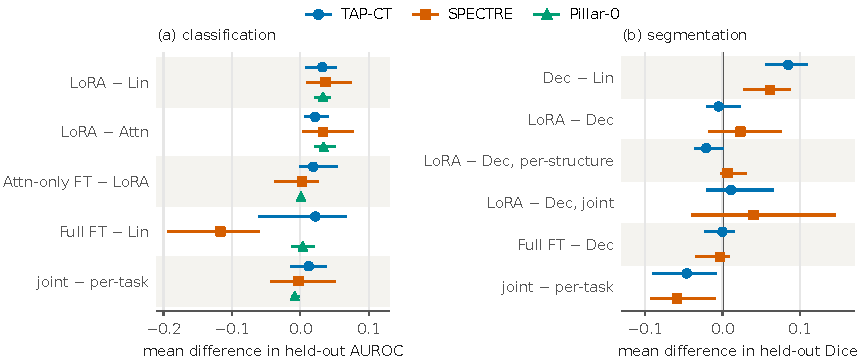
\includegraphics[width=\textwidth,height=0.74\textheight,keepaspectratio]{figures/fig_key.pdf}
\caption{Label-level mean difference in held-out AUROC (a) or Dice (b) for the comparisons of Table~\ref{tab:key}, per backbone, with the 95\% interval over cohorts, labels and held-out cases; 0 means no difference. A triangle at the axis edge marks an estimate beyond the axis, with its value printed. The SPECTRE Full FT $-$ Lin estimate includes runs that did not train.}
\label{fig:key}
\end{figure}

\begin{table}[H]
\centering
\caption{Classification headline: pooled held-out AUROC per backbone (mean over all label comparisons, $n$ = labels $\times$ \{per-task, joint\}), and per-label paired comparisons of LoRA against the linear probe and against full fine-tuning (DeLong, Benjamini--Hochberg; ``sig.'' = corrected $p<0.05$ in the stated direction). The mean gain of LoRA over the probe is similar for small and large held-out splits ($\numSigbysizeSmallMeandiff$ below 100 cases, $\numSigbysizeLargeMeandiff$ above 400) but significant in \numSigbysizeSmallSig\% and \numSigbysizeLargeSig\% of these comparisons; every comparison above 400 cases is from the hemorrhage cohort.}
\label{tab:headline}
\adjustbox{max width=\textwidth,max totalheight=0.8\textheight}{\footnotesize\begin{tabular}{lrccccrrrrrr}
\toprule
 & & \multicolumn{4}{c}{Pooled AUROC} & \multicolumn{3}{c}{LoRA vs.\ linear probe} & \multicolumn{3}{c}{LoRA vs.\ full fine-tuning} \\
\cmidrule(lr){3-6}\cmidrule(lr){7-9}\cmidrule(lr){10-12}
Backbone & $n$ & Lin & LoRA & Attn-only FT & Full FT & Mean $\Delta$ & LoRA better (\%) & sig.\ (\%) & Mean $\Delta$ & LoRA better (\%) & FT sig.\ better (\%) \\
\midrule
TAP-CT & 78 & 0.727 & 0.760 & 0.779 & 0.749 & +0.032 & 78 & 17 & +0.010 & 55 & 6 \\
SPECTRE & 66 & 0.718 & 0.755 & 0.757 & 0.601 & +0.037 & 74 & 9 & +0.153 & 94 & 2 \\
Pillar-0 & 12 & 0.887 & 0.920 & 0.922 & 0.891 & +0.033 & 92 & 83 & +0.029 & 100 & 0 \\
\bottomrule
\end{tabular}
}
\end{table}

\begin{table}[H]
\centering
\caption{Classification methods: trainable parameters of a single-label model as logged (head included; for Pillar-0 the count includes parameters of per-scale blocks that never run and receive no gradient, so the encoder parameters updated are about half, Figure~\ref{fig:arms}); mean rank within each of the \numRankSlotsN{} label--mode pairs ($\downarrow$; on SPECTRE among the ten methods that trained); share of pairs within 0.01 AUROC of the best method ($\uparrow$); mean AUROC deficit to the best method ($\downarrow$). \textbf{Bold}: best, \underline{underlined}: second best of each rank and score column. Full FT's pooled values exclude SPECTRE, where it did not train, so they are not comparable with the other methods' and are not marked. Choosing the method per label on the selection split finds the held-out best in \numSelectHit\% of pairs and lowers the mean deficit from $\numRegretAttnft$ (always attention-only fine-tuning) to $\numSelectRegret$, at eleven runs per label instead of one.}
\label{tab:methods}
\adjustbox{max width=\textwidth,max totalheight=0.8\textheight}{\footnotesize\begin{tabular}{lrrrccccrr}
\toprule
 & \multicolumn{3}{c}{Trainable parameters} & \multicolumn{4}{c}{Mean rank (1 = best)} & Within 0.01 & $\Delta$ to best \\
\cmidrule(lr){2-4}\cmidrule(lr){5-8}
Method & TAP-CT & SPECTRE & Pillar-0 & TAP-CT & SPECTRE & Pillar-0 & All & of best (\%) & (AUROC) \\
\midrule
Lin & 769 & 1081 & 1153 & 7.62 & 7.15 & 9.33 & 7.55 & 7 & 0.081 \\
Attn & 14.2\,M & 28.0\,M & 31.9\,M & 6.71 & 6.96 & 9.75 & 7.05 & 10 & 0.074 \\
LoRA & 14.8\,M & 30.4\,M & 32.4\,M & \underline{4.76} & 4.94 & 3.83 & \underline{4.76} & 23 & 0.046 \\
LoRA$_{\text{late}}$ & 14.4\,M & 29.1\,M & 32.1\,M & 5.46 & 5.50 & 7.17 & 5.61 & 17 & 0.054 \\
LoRA+ABMIL & 15.0\,M & 30.7\,M & 32.7\,M & 5.61 & \textbf{4.02} & 4.33 & 4.84 & \underline{26} & \underline{0.045} \\
DoRA & 14.8\,M & 30.5\,M & 32.5\,M & 5.50 & 4.72 & 3.67 & 5.03 & 19 & 0.049 \\
rsLoRA & 14.8\,M & 30.4\,M & 32.4\,M & 7.17 & 5.31 & \textbf{2.67} & 6.04 & 18 & 0.065 \\
Lin$\to$LoRA & 0.20\,M & 1.0\,M & 0.25\,M & 7.48 & 5.27 & 6.58 & 6.47 & 11 & 0.064 \\
Attn$\to$LoRA & 14.4\,M & 29.1\,M & 32.1\,M & 6.90 & 6.47 & 7.67 & 6.78 & 13 & 0.069 \\
Attn-only FT & 42.5\,M & 159\,M & 42.5\,M & \textbf{3.38} & \underline{4.67} & \underline{3.25} & \textbf{3.91} & \textbf{38} & \textbf{0.036} \\
Full FT & 101\,M & 425\,M & 76.7\,M & 5.44 & -- & 7.75 & 5.74 & 31 & 0.055 \\
\bottomrule
\end{tabular}
}
\end{table}

\begin{table}[H]
\centering
\caption{Label-level differences with 95\% intervals. Each label (or structure) counts once, with its per-task and joint differences averaged (except the two LoRA $-$ Dec sub-rows). Intervals are percentile bootstraps (4000 resamples) over cohort--backbone groups and labels within them, without and with a third stage that resamples the held-out cases of each drawn label (Appendix~\ref{app:stats}). Pillar-0 has one cohort, so its interval resamples labels and cases only. The last column counts the cohorts (datasets) with a positive mean difference.}
\label{tab:cis}
\adjustbox{max width=\textwidth,max totalheight=0.8\textheight}{\footnotesize\begin{tabular}{llrrccc}
\toprule
 & & & & \multicolumn{2}{c}{95\% interval, resampling} & \\
\cmidrule(lr){5-6}
Comparison & Backbone & $n$ & Mean & cohorts, labels & + cases & Cohorts $>0$ \\
\midrule
LoRA $-$ Lin & all & 78 & $+0.034$ & [$+0.019$, $+0.049$] & [$+0.017$, $+0.052$] & 9/10 \\
LoRA $-$ Lin & TAP-CT & 39 & $+0.032$ & [$+0.009$, $+0.049$] & [$+0.007$, $+0.053$] & 4/5 \\
LoRA $-$ Lin & SPECTRE & 33 & $+0.037$ & [$+0.013$, $+0.068$] & [$+0.009$, $+0.075$] & 4/4 \\
LoRA $-$ Lin & Pillar-0 & 6 & $+0.033$ & [$+0.021$, $+0.042$] & [$+0.021$, $+0.044$] & 1/1 \\
\addlinespace[2pt]
LoRA $-$ Attn & all & 78 & $+0.027$ & [$+0.013$, $+0.047$] & [$+0.012$, $+0.048$] & 10/10 \\
LoRA $-$ Attn & TAP-CT & 39 & $+0.022$ & [$+0.009$, $+0.039$] & [$+0.006$, $+0.042$] & 5/5 \\
LoRA $-$ Attn & SPECTRE & 33 & $+0.033$ & [$+0.007$, $+0.074$] & [$+0.003$, $+0.078$] & 4/4 \\
LoRA $-$ Attn & Pillar-0 & 6 & $+0.034$ & [$+0.021$, $+0.051$] & [$+0.021$, $+0.052$] & 1/1 \\
\addlinespace[2pt]
Attn-only FT $-$ LoRA & all & 78 & $+0.011$ & [$-0.005$, $+0.026$] & [$-0.007$, $+0.029$] & 7/10 \\
Attn-only FT $-$ LoRA & TAP-CT & 39 & $+0.019$ & [$+0.002$, $+0.053$] & [$-0.001$, $+0.054$] & 4/5 \\
Attn-only FT $-$ LoRA & SPECTRE & 33 & $+0.002$ & [$-0.037$, $+0.023$] & [$-0.037$, $+0.026$] & 2/4 \\
Attn-only FT $-$ LoRA & Pillar-0 & 6 & $+0.001$ & [$0.000$, $+0.003$] & [$-0.002$, $+0.004$] & 1/1 \\
\addlinespace[2pt]
Full FT $-$ Lin & all & 78 & $-0.038$ & [$-0.101$, $+0.017$] & [$-0.103$, $+0.019$] & 5/10 \\
Full FT $-$ Lin & TAP-CT & 39 & $+0.022$ & [$-0.057$, $+0.064$] & [$-0.061$, $+0.068$] & 4/5 \\
Full FT $-$ Lin & SPECTRE & 33 & $-0.117$ & [$-0.195$, $-0.063$] & [$-0.195$, $-0.059$] & 0/4 \\
Full FT $-$ Lin & Pillar-0 & 6 & $+0.004$ & [$-0.011$, $+0.019$] & [$-0.013$, $+0.021$] & 1/1 \\
\addlinespace[2pt]
Joint $-$ per-task & all & 78 & $+0.004$ & [$-0.017$, $+0.027$] & [$-0.021$, $+0.030$] & 6/10 \\
Joint $-$ per-task & TAP-CT & 39 & $+0.012$ & [$-0.005$, $+0.032$] & [$-0.014$, $+0.038$] & 3/5 \\
Joint $-$ per-task & SPECTRE & 33 & $-0.003$ & [$-0.035$, $+0.049$] & [$-0.044$, $+0.051$] & 3/4 \\
Joint $-$ per-task & Pillar-0 & 6 & $-0.008$ & [$-0.012$, $-0.003$] & [$-0.013$, $-0.001$] & 0/1 \\
\addlinespace[2pt]
Attn $-$ Lin & all & 78 & $+0.007$ & [$-0.010$, $+0.021$] & [$-0.012$, $+0.023$] & 5/10 \\
Attn $-$ Lin & TAP-CT & 39 & $+0.011$ & [$-0.013$, $+0.027$] & [$-0.014$, $+0.029$] & 3/5 \\
Attn $-$ Lin & SPECTRE & 33 & $+0.004$ & [$-0.022$, $+0.030$] & [$-0.030$, $+0.035$] & 2/4 \\
Attn $-$ Lin & Pillar-0 & 6 & $-0.001$ & [$-0.012$, $+0.007$] & [$-0.014$, $+0.008$] & 0/1 \\
\addlinespace[2pt]
Attn-only FT $-$ Lin & all & 78 & $+0.045$ & [$+0.027$, $+0.062$] & [$+0.024$, $+0.065$] & 8/10 \\
Attn-only FT $-$ Lin & TAP-CT & 39 & $+0.051$ & [$+0.026$, $+0.078$] & [$+0.023$, $+0.080$] & 4/5 \\
Attn-only FT $-$ Lin & SPECTRE & 33 & $+0.039$ & [$-0.001$, $+0.067$] & [$-0.003$, $+0.075$] & 3/4 \\
Attn-only FT $-$ Lin & Pillar-0 & 6 & $+0.034$ & [$+0.022$, $+0.044$] & [$+0.021$, $+0.046$] & 1/1 \\
\addlinespace[2pt]
Attn-only FT $-$ Attn & all & 78 & $+0.038$ & [$+0.020$, $+0.060$] & [$+0.018$, $+0.062$] & 10/10 \\
Attn-only FT $-$ Attn & TAP-CT & 39 & $+0.041$ & [$+0.018$, $+0.078$] & [$+0.014$, $+0.082$] & 5/5 \\
Attn-only FT $-$ Attn & SPECTRE & 33 & $+0.035$ & [$+0.001$, $+0.069$] & [$-0.002$, $+0.075$] & 4/4 \\
Attn-only FT $-$ Attn & Pillar-0 & 6 & $+0.036$ & [$+0.022$, $+0.052$] & [$+0.021$, $+0.053$] & 1/1 \\
\addlinespace[2pt]
LoRA $-$ Lin, without FDG-PET/CT and COVID-CTset & all & 68 & $+0.037$ & [$+0.023$, $+0.054$] & [$+0.019$, $+0.057$] & 8/8 \\
LoRA $-$ Lin, without FDG-PET/CT and COVID-CTset & TAP-CT & 34 & $+0.035$ & [$+0.016$, $+0.053$] & [$+0.013$, $+0.056$] & 4/4 \\
LoRA $-$ Lin, without FDG-PET/CT and COVID-CTset & SPECTRE & 28 & $+0.041$ & [$+0.015$, $+0.078$] & [$+0.009$, $+0.085$] & 3/3 \\
LoRA $-$ Lin, without FDG-PET/CT and COVID-CTset & Pillar-0 & 6 & $+0.033$ & [$+0.021$, $+0.042$] & [$+0.020$, $+0.044$] & 1/1 \\
\addlinespace[2pt]
Dec $-$ Lin & all & 74 & $+0.073$ & [$+0.049$, $+0.093$] & [$+0.049$, $+0.092$] & 10/10 \\
Dec $-$ Lin & TAP-CT & 37 & $+0.085$ & [$+0.055$, $+0.109$] & [$+0.055$, $+0.109$] & 5/5 \\
Dec $-$ Lin & SPECTRE & 37 & $+0.061$ & [$+0.028$, $+0.089$] & [$+0.027$, $+0.088$] & 5/5 \\
\addlinespace[2pt]
LoRA $-$ Dec & all & 74 & $+0.009$ & [$-0.014$, $+0.046$] & [$-0.015$, $+0.046$] & 8/10 \\
LoRA $-$ Dec & TAP-CT & 37 & $-0.005$ & [$-0.021$, $+0.023$] & [$-0.021$, $+0.024$] & 4/5 \\
LoRA $-$ Dec & SPECTRE & 37 & $+0.023$ & [$-0.017$, $+0.079$] & [$-0.018$, $+0.076$] & 4/5 \\
\addlinespace[2pt]
\quad per-structure models & all & 74 & $-0.007$ & [$-0.021$, $+0.009$] & [$-0.022$, $+0.009$] & 7/10 \\
\quad per-structure models & TAP-CT & 37 & $-0.021$ & [$-0.035$, $+0.002$] & [$-0.036$, $+0.002$] & 2/5 \\
\quad per-structure models & SPECTRE & 37 & $+0.006$ & [$-0.001$, $+0.028$] & [$-0.003$, $+0.031$] & 5/5 \\
\addlinespace[2pt]
\quad joint models & all & 74 & $+0.026$ & [$-0.020$, $+0.092$] & [$-0.021$, $+0.093$] & 8/10 \\
\quad joint models & TAP-CT & 37 & $+0.011$ & [$-0.019$, $+0.067$] & [$-0.021$, $+0.066$] & 4/5 \\
\quad joint models & SPECTRE & 37 & $+0.040$ & [$-0.038$, $+0.148$] & [$-0.039$, $+0.147$] & 4/5 \\
\addlinespace[2pt]
Full FT $-$ Dec & all & 74 & $-0.002$ & [$-0.017$, $+0.009$] & [$-0.018$, $+0.009$] & 6/10 \\
Full FT $-$ Dec & TAP-CT & 37 & $0.000$ & [$-0.025$, $+0.015$] & [$-0.024$, $+0.016$] & 4/5 \\
Full FT $-$ Dec & SPECTRE & 37 & $-0.003$ & [$-0.033$, $+0.008$] & [$-0.035$, $+0.009$] & 2/5 \\
\addlinespace[2pt]
Joint $-$ per-task & all & 74 & $-0.052$ & [$-0.082$, $-0.021$] & [$-0.082$, $-0.022$] & 0/10 \\
Joint $-$ per-task & TAP-CT & 37 & $-0.046$ & [$-0.088$, $-0.009$] & [$-0.090$, $-0.008$] & 0/5 \\
Joint $-$ per-task & SPECTRE & 37 & $-0.058$ & [$-0.092$, $-0.010$] & [$-0.093$, $-0.009$] & 0/5 \\
\bottomrule
\end{tabular}
}
\end{table}

\begin{table}[H]
\centering
\caption{Per-label paired comparisons of held-out AUROC against the linear probe and against full fine-tuning, over the per-task and joint modes (DeLong test; Benjamini--Hochberg correction within each baseline over the comparisons of TAP-CT, SPECTRE and Pillar-0). ``Better'' is the share of label--mode pairs in which the method's AUROC exceeds the baseline's; ``Sig.'' the share in which, in addition, the corrected $p<0.05$. SPECTRE Full FT did not train.}
\label{tab:paired}
\adjustbox{max width=\textwidth,max totalheight=0.8\textheight}{\footnotesize\begin{tabular}{lllrrrrr}
\toprule
Backbone & Baseline & Method & Label--mode pairs & Mean $\Delta$AUROC & Better (\%) & Sig.\ better (\%) & Sig.\ worse (\%) \\
\midrule
TAP-CT & vs Lin & Attn & 78 & +0.011 & 59 & 4 & 0 \\
 &  & LoRA & 78 & +0.032 & 78 & 17 & 0 \\
 &  & LoRA$_{\text{late}}$ & 78 & +0.023 & 69 & 14 & 1 \\
 &  & LoRA+ABMIL & 78 & +0.024 & 68 & 12 & 1 \\
 &  & DoRA & 78 & +0.028 & 68 & 17 & 0 \\
 &  & rsLoRA & 78 & +0.003 & 55 & 5 & 5 \\
 &  & Lin$\to$LoRA & 78 & +0.001 & 51 & 5 & 1 \\
 &  & Attn$\to$LoRA & 78 & +0.008 & 56 & 9 & 0 \\
 &  & Attn-only FT & 78 & +0.051 & 83 & 24 & 0 \\
 &  & Full FT & 78 & +0.022 & 72 & 13 & 8 \\
\addlinespace[2pt]
TAP-CT & vs Full FT & Lin & 78 & $-$0.022 & 28 & 12 & 17 \\
 &  & Attn & 78 & $-$0.011 & 40 & 10 & 18 \\
 &  & LoRA & 78 & +0.010 & 55 & 18 & 6 \\
 &  & LoRA$_{\text{late}}$ & 78 & +0.001 & 44 & 18 & 6 \\
 &  & LoRA+ABMIL & 78 & +0.002 & 45 & 17 & 12 \\
 &  & DoRA & 78 & +0.006 & 51 & 17 & 9 \\
 &  & rsLoRA & 78 & $-$0.019 & 47 & 13 & 22 \\
 &  & Lin$\to$LoRA & 78 & $-$0.021 & 31 & 9 & 18 \\
 &  & Attn$\to$LoRA & 78 & $-$0.014 & 38 & 13 & 15 \\
 &  & Attn-only FT & 78 & +0.029 & 63 & 23 & 5 \\
\addlinespace[2pt]
SPECTRE & vs Lin & Attn & 66 & +0.004 & 50 & 3 & 2 \\
 &  & LoRA & 66 & +0.037 & 74 & 9 & 0 \\
 &  & LoRA$_{\text{late}}$ & 66 & +0.034 & 65 & 5 & 0 \\
 &  & LoRA+ABMIL & 66 & +0.052 & 77 & 12 & 2 \\
 &  & DoRA & 66 & +0.037 & 77 & 8 & 0 \\
 &  & rsLoRA & 66 & +0.028 & 70 & 9 & 0 \\
 &  & Lin$\to$LoRA & 66 & +0.035 & 71 & 6 & 0 \\
 &  & Attn$\to$LoRA & 66 & +0.016 & 59 & 6 & 2 \\
 &  & Attn-only FT & 66 & +0.039 & 70 & 3 & 3 \\
 &  & Full FT & 66 & $-$0.117 & 21 & 0 & 32 \\
\addlinespace[2pt]
SPECTRE & vs Full FT & Lin & 66 & +0.117 & 79 & 33 & 0 \\
 &  & Attn & 66 & +0.121 & 86 & 35 & 0 \\
 &  & LoRA & 66 & +0.153 & 94 & 44 & 2 \\
 &  & LoRA$_{\text{late}}$ & 66 & +0.151 & 95 & 44 & 0 \\
 &  & LoRA+ABMIL & 66 & +0.168 & 94 & 52 & 0 \\
 &  & DoRA & 66 & +0.154 & 92 & 44 & 2 \\
 &  & rsLoRA & 66 & +0.145 & 89 & 39 & 0 \\
 &  & Lin$\to$LoRA & 66 & +0.152 & 94 & 41 & 0 \\
 &  & Attn$\to$LoRA & 66 & +0.133 & 88 & 44 & 0 \\
 &  & Attn-only FT & 66 & +0.156 & 89 & 48 & 0 \\
\addlinespace[2pt]
Pillar-0 & vs Lin & Attn & 12 & $-$0.001 & 42 & 33 & 8 \\
 &  & LoRA & 12 & +0.033 & 92 & 83 & 0 \\
 &  & LoRA$_{\text{late}}$ & 12 & +0.016 & 75 & 67 & 0 \\
 &  & LoRA+ABMIL & 12 & +0.026 & 83 & 75 & 8 \\
 &  & DoRA & 12 & +0.034 & 92 & 83 & 0 \\
 &  & rsLoRA & 12 & +0.032 & 100 & 83 & 0 \\
 &  & Lin$\to$LoRA & 12 & +0.022 & 100 & 83 & 0 \\
 &  & Attn$\to$LoRA & 12 & +0.013 & 92 & 58 & 0 \\
 &  & Attn-only FT & 12 & +0.034 & 92 & 83 & 0 \\
 &  & Full FT & 12 & +0.004 & 67 & 50 & 17 \\
\addlinespace[2pt]
Pillar-0 & vs Full FT & Lin & 12 & $-$0.004 & 33 & 17 & 50 \\
 &  & Attn & 12 & $-$0.005 & 33 & 17 & 58 \\
 &  & LoRA & 12 & +0.029 & 100 & 67 & 0 \\
 &  & LoRA$_{\text{late}}$ & 12 & +0.012 & 58 & 33 & 25 \\
 &  & LoRA+ABMIL & 12 & +0.022 & 58 & 58 & 8 \\
 &  & DoRA & 12 & +0.030 & 83 & 67 & 0 \\
 &  & rsLoRA & 12 & +0.028 & 92 & 67 & 0 \\
 &  & Lin$\to$LoRA & 12 & +0.018 & 67 & 42 & 25 \\
 &  & Attn$\to$LoRA & 12 & +0.009 & 50 & 33 & 25 \\
 &  & Attn-only FT & 12 & +0.030 & 100 & 83 & 0 \\
\addlinespace[2pt]
\bottomrule
\end{tabular}
}
\end{table}

\begin{table}[H]
\centering
\caption{Per-structure paired comparisons of held-out Dice over the per-structure and joint modes against the linear probe and the frozen decoder (paired bootstrap of the mean per-case difference, 4000 resamples; Benjamini--Hochberg correction within each baseline). Pairing keeps the cases on which a structure enters the Dice of both methods (present in the reference or in either prediction), so the mean differences here can differ from the differences of structure means in Table~\ref{tab:seg}.}
\label{tab:segpaired}
\adjustbox{max width=\textwidth,max totalheight=0.8\textheight}{\footnotesize\begin{tabular}{lllrrrrr}
\toprule
Backbone & Baseline & Method & Pairs & Mean $\Delta$Dice & Better (\%) & Sig.\ better (\%) & Sig.\ worse (\%) \\
\midrule
TAP-CT & vs Lin & Dec & 74 & +0.086 & 96 & 93 & 4 \\
 &  & LoRA & 74 & +0.088 & 96 & 93 & 3 \\
 &  & LoRA$_{\text{late}}$ & 59 & +0.077 & 95 & 92 & 5 \\
 &  & DoRA & 59 & +0.078 & 95 & 90 & 5 \\
 &  & Full FT & 74 & +0.085 & 93 & 93 & 7 \\
 &  & Dec$\to$LoRA & 59 & +0.066 & 92 & 88 & 8 \\
\addlinespace[2pt]
TAP-CT & vs Dec & Lin & 74 & -0.086 & 4 & 4 & 93 \\
 &  & LoRA & 74 & +0.002 & 54 & 31 & 30 \\
 &  & LoRA$_{\text{late}}$ & 59 & -0.006 & 53 & 29 & 32 \\
 &  & DoRA & 59 & -0.006 & 53 & 25 & 25 \\
 &  & Full FT & 74 & -0.001 & 76 & 53 & 8 \\
 &  & Dec$\to$LoRA & 59 & -0.017 & 29 & 7 & 44 \\
\addlinespace[2pt]
SPECTRE & vs Lin & Dec & 74 & +0.061 & 92 & 86 & 5 \\
 &  & LoRA & 74 & +0.095 & 93 & 93 & 4 \\
 &  & LoRA$_{\text{late}}$ & 59 & +0.079 & 92 & 90 & 5 \\
 &  & DoRA & 59 & +0.088 & 93 & 90 & 7 \\
 &  & Full FT & 74 & +0.059 & 89 & 81 & 8 \\
 &  & Dec$\to$LoRA & 59 & +0.051 & 90 & 85 & 7 \\
\addlinespace[2pt]
SPECTRE & vs Dec & Lin & 74 & -0.061 & 8 & 5 & 86 \\
 &  & LoRA & 74 & +0.034 & 80 & 57 & 8 \\
 &  & LoRA$_{\text{late}}$ & 59 & +0.032 & 69 & 46 & 8 \\
 &  & DoRA & 59 & +0.041 & 76 & 54 & 12 \\
 &  & Full FT & 74 & -0.002 & 54 & 38 & 20 \\
 &  & Dec$\to$LoRA & 59 & +0.004 & 69 & 20 & 12 \\
\addlinespace[2pt]
\bottomrule
\end{tabular}
}
\end{table}

\begin{figure}[H]
\centering
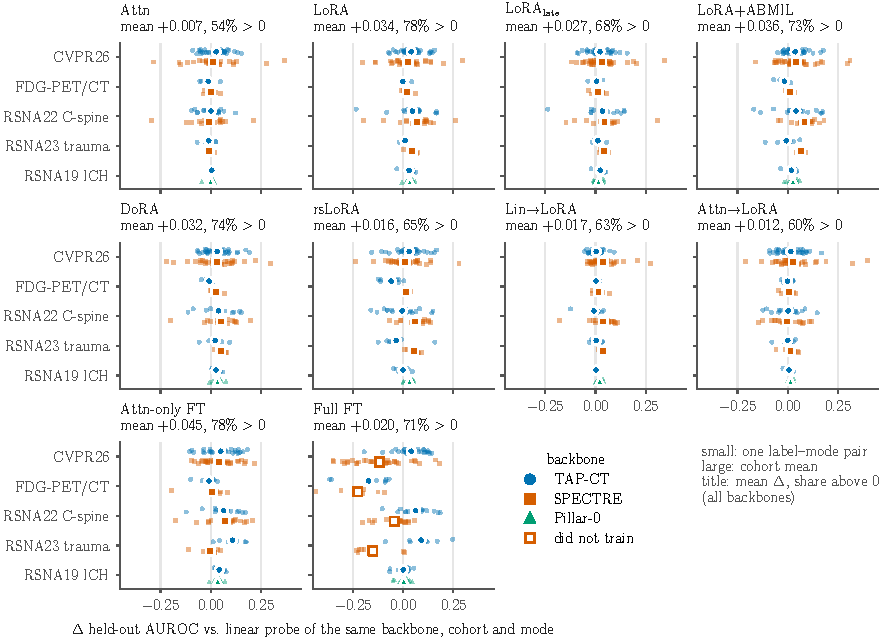
\includegraphics[width=\textwidth,height=0.74\textheight,keepaspectratio]{figures/fig_methods.pdf}
\caption{Per-label change in held-out AUROC of each classification method relative to the linear probe of the same backbone, cohort and mode, one panel per method; rows are cohorts, color is the backbone, small markers are single label--mode comparisons and large markers the mean per cohort and backbone. Titles give the mean change and the share above zero over the pairs of all three backbones that trained. SPECTRE Full FT did not train; its cohort means are drawn open and left out of the title.}
\label{fig:methods}
\end{figure}

\begin{figure}[H]
\centering
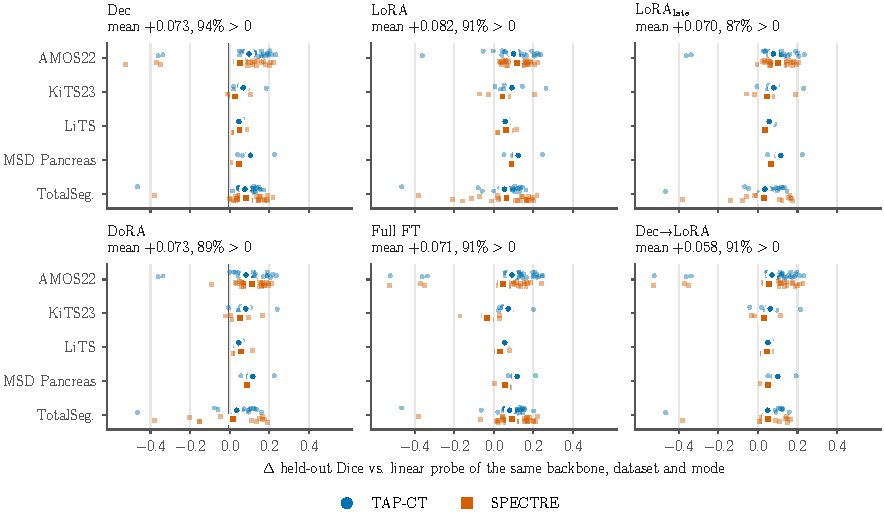
\includegraphics[width=\textwidth,height=0.74\textheight,keepaspectratio]{figures/fig_seg_methods.pdf}
\caption{Per-structure change in held-out Dice of each segmentation method relative to the linear probe of the same backbone, dataset and mode, one panel per method; rows are datasets, color is the backbone, small markers are single structure--mode comparisons and large markers the mean per dataset and backbone.}
\label{fig:segmethods}
\end{figure}

\begin{table}[H]
\centering
\caption{Encoder adaptation on top of the frozen decoder per dataset, backbone and mode: difference of structure-mean held-out Dice. Joint rows of AMOS22 and TotalSegmentator use the 24\,000-step schedule; the 8000-step rows show the same models under the shared budget.}
\label{tab:segmodes}
\adjustbox{max width=\textwidth,max totalheight=0.8\textheight}{\footnotesize\begin{tabular}{llrrrr}
\toprule
 & & \multicolumn{2}{c}{LoRA $-$ Dec} & \multicolumn{2}{c}{Full FT $-$ Dec} \\
\cmidrule(lr){3-4}\cmidrule(lr){5-6}
Dataset & Mode & TAP-CT & SPECTRE & TAP-CT & SPECTRE \\
\midrule
AMOS22 (15) & per-structure & $-0.026$ & $+0.004$ & $+0.012$ & $-0.016$ \\
 & joint & $+0.031$ & $+0.126$ & $-0.027$ & $+0.011$ \\
 & joint, 8000 steps & $-0.125$ & $-0.071$ & $+0.007$ & $+0.010$ \\
KiTS23 (3) & per-structure & $-0.021$ & $+0.014$ & $+0.005$ & $-0.071$ \\
 & joint & $+0.068$ & $+0.016$ & $+0.006$ & $-0.052$ \\
LiTS (2) & per-structure & $+0.007$ & $+0.015$ & $+0.001$ & $-0.002$ \\
 & joint & $+0.016$ & $+0.011$ & $+0.016$ & $-0.030$ \\
MSD Pancreas (2) & per-structure & $+0.013$ & $+0.047$ & $+0.021$ & $+0.000$ \\
 & joint & $+0.025$ & $+0.037$ & $+0.008$ & $+0.016$ \\
TotalSegmentator (15) & per-structure & $-0.024$ & $+0.001$ & $-0.011$ & $-0.009$ \\
 & joint & $-0.022$ & $-0.036$ & $+0.017$ & $+0.025$ \\
 & joint, 8000 steps & $-0.199$ & $-0.254$ & $+0.022$ & $+0.037$ \\
\bottomrule
\end{tabular}
}
\end{table}

\begin{table}[H]
\centering
\caption{The training budget of the 15-structure joint models (AMOS22, TotalSegmentator): held-out Dice, mean over structures, for one model per structure (8000 steps each), one joint model under the shared 8000 steps, and one joint model with three times the steps (Dec$\to$LoRA: 12\,000 + 12\,000).}
\label{tab:segbudget}
\adjustbox{max width=\textwidth,max totalheight=0.8\textheight}{\footnotesize\begin{tabular}{lllccccccc}
\toprule
Dataset & Backbone & Training & Lin & Dec & LoRA & LoRA$_{\text{late}}$ & DoRA & Full FT & Dec$\to$LoRA \\
\midrule
AMOS22 & TAP-CT & per-structure, 8000 steps & 0.658 & 0.793 & 0.767 & 0.764 & 0.761 & 0.805 & 0.791 \\
AMOS22 & TAP-CT & joint, 8000 steps & 0.632 & 0.595 & 0.470 & 0.412 & 0.455 & 0.602 & 0.591 \\
AMOS22 & TAP-CT & joint, 24\,000 steps & 0.646 & 0.708 & 0.739 & 0.698 & 0.708 & 0.681 & 0.656 \\
\addlinespace[2pt]
AMOS22 & SPECTRE & per-structure, 8000 steps & 0.683 & 0.808 & 0.812 & 0.806 & 0.814 & 0.792 & 0.814 \\
AMOS22 & SPECTRE & joint, 8000 steps & 0.670 & 0.640 & 0.568 & 0.527 & 0.567 & 0.649 & 0.627 \\
AMOS22 & SPECTRE & joint, 24\,000 steps & 0.682 & 0.658 & 0.784 & 0.764 & 0.775 & 0.669 & 0.664 \\
\addlinespace[2pt]
TotalSegmentator & TAP-CT & per-structure, 8000 steps & 0.747 & 0.843 & 0.819 & -- & -- & 0.832 & -- \\
TotalSegmentator & TAP-CT & joint, 8000 steps & 0.731 & 0.781 & 0.583 & 0.594 & 0.591 & 0.803 & 0.776 \\
TotalSegmentator & TAP-CT & joint, 24\,000 steps & 0.740 & 0.798 & 0.776 & 0.776 & 0.776 & 0.815 & 0.790 \\
\addlinespace[2pt]
TotalSegmentator & SPECTRE & per-structure, 8000 steps & 0.731 & 0.848 & 0.848 & -- & -- & 0.838 & -- \\
TotalSegmentator & SPECTRE & joint, 8000 steps & 0.712 & 0.679 & 0.425 & 0.387 & 0.408 & 0.716 & 0.637 \\
TotalSegmentator & SPECTRE & joint, 24\,000 steps & 0.722 & 0.770 & 0.733 & 0.752 & 0.736 & 0.795 & 0.772 \\
\addlinespace[2pt]
\bottomrule
\end{tabular}
}
\end{table}

\begin{figure}[H]
\centering
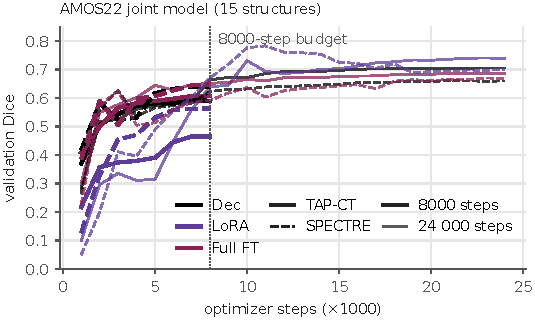
\includegraphics[width=0.62\textwidth,height=0.74\textheight,keepaspectratio]{figures/fig_seg_budget.pdf}
\caption{Validation Dice during training of the 15-structure AMOS22 joint model with the frozen decoder, LoRA and full fine-tuning, on TAP-CT (solid) and SPECTRE (dashed); thick lines stop at the shared 8000 steps, thin lines run 24\,000 steps.}
\label{fig:segbudget}
\end{figure}

\begin{figure}[H]
\centering
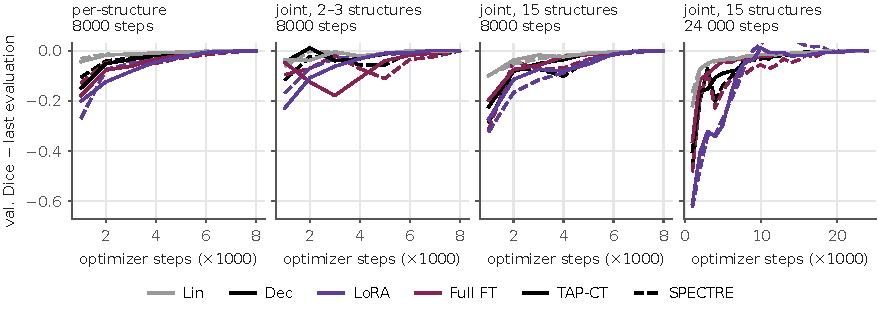
\includegraphics[width=\textwidth,height=0.74\textheight,keepaspectratio]{figures/fig_seg_convergence.pdf}
\caption{Validation Dice at each evaluation minus that at the run's last evaluation, median over the runs of each schedule group, for Lin, Dec, LoRA and Full FT on TAP-CT (solid) and SPECTRE (dashed). Every curve ends at zero by construction; a curve still rising at the right edge had not converged.}
\label{fig:segconv}
\end{figure}

\begin{figure}[H]
\centering
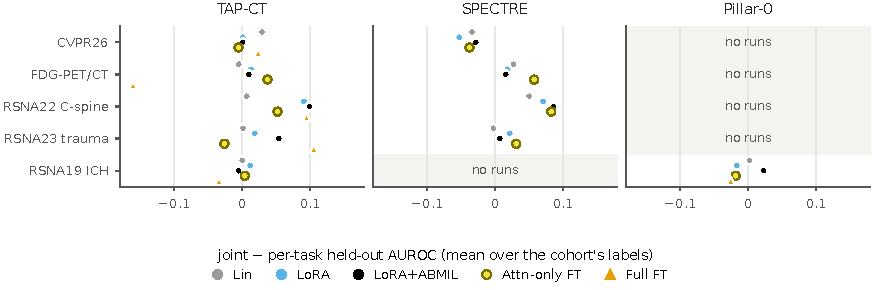
\includegraphics[width=\textwidth,height=0.74\textheight,keepaspectratio]{figures/fig_joint.pdf}
\caption{Joint minus per-task held-out AUROC, mean over the labels of each cohort, for Lin, LoRA, LoRA+ABMIL, Attn-only FT and Full FT, per backbone (SPECTRE Full FT, which did not train, is not shown). Right of zero favors one joint model per cohort.}
\label{fig:joint}
\end{figure}
\begin{figure}[H]
\centering
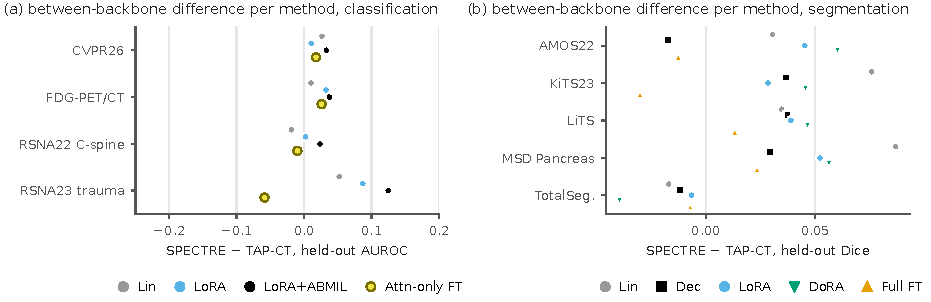
\includegraphics[width=\textwidth,height=0.74\textheight,keepaspectratio]{figures/fig_bbgap.pdf}
\caption{Between-backbone difference per method: SPECTRE minus TAP-CT held-out AUROC per cohort (a) and held-out Dice per dataset (b), on the same labels or structures and modes. SPECTRE Full FT, which did not train in classification, is not shown in (a). Dice in (b) is computed on each backbone's own grid, so part of a difference can come from the grid.}
\label{fig:bbgap}
\end{figure}

\begin{table}[H]
\centering
\caption{Median over label--mode pairs of the standard deviation of the held-out probabilities per backbone and method (the did-not-train rule flags values below \numSpreadMinValue{}; applied to TAP-CT, SPECTRE and Pillar-0 only).}
\label{tab:spread}
\adjustbox{max width=\textwidth,max totalheight=0.8\textheight}{\small\setlength{\tabcolsep}{3pt}
\begin{tabular}{lccccccccccc}
\toprule
Backbone & Lin & Attn & LoRA & LoRA$_{\text{late}}$ & LoRA+ABMIL & DoRA & rsLoRA & Lin$\to$LoRA & Attn$\to$LoRA & Attn-only FT & Full FT \\
\midrule
TAP-CT & 0.227 & 0.239 & 0.239 & 0.235 & 0.233 & 0.237 & 0.167 & 0.222 & 0.225 & 0.247 & 0.170 \\
SPECTRE & 0.187 & 0.114 & 0.161 & 0.185 & 0.187 & 0.185 & 0.150 & 0.178 & 0.129 & 0.148 & \textbf{0.004}$^{\dagger}$ \\
Pillar-0 & 0.294 & 0.321 & 0.359 & 0.350 & 0.352 & 0.354 & 0.359 & 0.337 & 0.338 & 0.355 & 0.347 \\
\bottomrule
\end{tabular}
}
\end{table}

\clearpage
\section{Seed repeats, full fine-tuning settings and compute-matched models}
\label{app:revision}

\begin{table}[H]
\centering
\caption{Held-out AUROC of the joint classification models across seeds 42, 43 and 44: mean over the cohort's labels, given as mean $\pm$ standard deviation over the seeds (their number in brackets), and the number of seeds in which the mean label difference between two methods is positive. SPECTRE Full FT, which did not train, has seed 42 only.}
\label{tab:seedscls}
\adjustbox{max width=\textwidth,max totalheight=0.8\textheight}{\scriptsize\begin{tabular}{lrrrrcc}
\toprule
Cohort & Lin & LoRA & Attn-only FT & Full FT & \begin{tabular}[b]{@{}c@{}}LoRA\\$>$ Lin\end{tabular} & \begin{tabular}[b]{@{}c@{}}Attn-only FT\\$>$ LoRA\end{tabular} \\
\midrule
\multicolumn{7}{@{}l}{\textit{TAP-CT}} \\
CVPR26 & 0.705 $\pm$ .004 (3) & 0.719 $\pm$ .016 (3) & 0.740 $\pm$ .009 (3) & 0.711 $\pm$ .029 (3) & 2/3 & 3/3 \\
FDG-PET/CT & 0.860 $\pm$ .003 (3) & 0.864 $\pm$ .008 (3) & 0.875 $\pm$ .012 (3) & 0.661 $\pm$ .130 (3) & 2/3 & 3/3 \\
RSNA23 trauma & 0.738 $\pm$ .008 (3) & 0.760 $\pm$ .002 (3) & 0.842 $\pm$ .030 (3) & 0.793 $\pm$ .157 (3) & 3/3 & 3/3 \\
RSNA22 C-spine & 0.623 $\pm$ .006 (3) & 0.659 $\pm$ .050 (3) & 0.691 $\pm$ .019 (3) & 0.695 $\pm$ .035 (3) & 2/3 & 2/3 \\
RSNA19 ICH & 0.871 $\pm$ .002 (3) & 0.896 $\pm$ .009 (3) & 0.904 $\pm$ .019 (3) & 0.836 $\pm$ .086 (3) & 3/3 & 2/3 \\
\multicolumn{7}{@{}l}{\textit{SPECTRE}} \\
CVPR26 & 0.711 $\pm$ .008 (3) & 0.741 $\pm$ .024 (3) & 0.759 $\pm$ .023 (3) & 0.575 (1) & 3/3 & 3/3 \\
FDG-PET/CT & 0.887 $\pm$ .003 (3) & 0.901 $\pm$ .000 (3) & 0.910 $\pm$ .006 (3) & 0.673 (1) & 3/3 & 3/3 \\
RSNA23 trauma & 0.792 $\pm$ .004 (3) & 0.846 $\pm$ .001 (3) & 0.834 $\pm$ .028 (3) & 0.654 (1) & 3/3 & 1/3 \\
RSNA22 C-spine & 0.592 $\pm$ .046 (3) & 0.696 $\pm$ .009 (3) & 0.683 $\pm$ .052 (3) & 0.554 (1) & 3/3 & 2/3 \\
\multicolumn{7}{@{}l}{\textit{Pillar-0}} \\
RSNA19 ICH & 0.888 $\pm$ .000 (3) & 0.916 $\pm$ .004 (3) & 0.921 $\pm$ .007 (3) & 0.894 $\pm$ .015 (3) & 3/3 & 3/3 \\
\bottomrule
\end{tabular}
}
\end{table}

\begin{table}[H]
\centering
\caption{Segmentation across seeds: held-out Dice of the joint models (AMOS22 and TotalSegmentator: 24\,000 steps), mean over structures, as in Table~\ref{tab:seedscls}.}
\label{tab:seedsseg}
\adjustbox{max width=\textwidth,max totalheight=0.8\textheight}{\footnotesize\begin{tabular}{lrrrcc}
\toprule
Dataset & Dec & LoRA & Full FT & \begin{tabular}[b]{@{}c@{}}LoRA\\$>$ Dec\end{tabular} & \begin{tabular}[b]{@{}c@{}}Full FT\\$>$ Dec\end{tabular} \\
\midrule
\multicolumn{6}{@{}l}{\textit{TAP-CT}} \\
AMOS22 & 0.675 $\pm$ .029 (3) & 0.709 $\pm$ .059 (3) & 0.680 $\pm$ .001 (3) & 2/3 & 2/3 \\
KiTS23 & 0.516 $\pm$ .003 (3) & 0.576 $\pm$ .005 (3) & 0.529 $\pm$ .014 (3) & 3/3 & 3/3 \\
LiTS & 0.715 $\pm$ .016 (3) & 0.718 $\pm$ .004 (3) & 0.717 $\pm$ .007 (3) & 2/3 & 2/3 \\
MSD Pancreas & 0.480 $\pm$ .002 (3) & 0.496 $\pm$ .009 (3) & 0.468 $\pm$ .027 (3) & 3/3 & 2/3 \\
TotalSegmentator & 0.783 $\pm$ .026 (3) & 0.773 $\pm$ .008 (3) & 0.815 $\pm$ .000 (3) & 1/3 & 3/3 \\
\multicolumn{6}{@{}l}{\textit{SPECTRE}} \\
AMOS22 & 0.658 $\pm$ .000 (3) & 0.775 $\pm$ .011 (3) & 0.669 $\pm$ .003 (3) & 3/3 & 3/3 \\
KiTS23 & 0.579 $\pm$ .010 (3) & 0.616 $\pm$ .024 (3) & 0.529 $\pm$ .015 (3) & 3/3 & 0/3 \\
LiTS & 0.741 $\pm$ .001 (3) & 0.740 $\pm$ .012 (3) & 0.707 $\pm$ .019 (3) & 1/3 & 0/3 \\
MSD Pancreas & 0.518 $\pm$ .004 (3) & 0.551 $\pm$ .008 (3) & 0.517 $\pm$ .011 (3) & 3/3 & 1/3 \\
TotalSegmentator & 0.741 $\pm$ .025 (3) & 0.752 $\pm$ .020 (3) & 0.762 $\pm$ .028 (3) & 2/3 & 3/3 \\
\bottomrule
\end{tabular}
}
\end{table}

\begin{table}[H]
\centering
\caption{Held-out AUROC of the joint classification models under the default and three alternative full fine-tuning settings, mean over the cohort's labels, next to Lin and LoRA. \textbf{Bold}: the setting selected for the backbone, by the best mean selection-split AUROC over its cohorts; it need not have the best held-out value of its row. Grey: runs whose held-out predictions barely vary (median over labels of the standard deviation of the predicted probabilities below \numSpreadMinValue{}).}
\label{tab:fullftfix}
\adjustbox{max width=\textwidth,max totalheight=0.8\textheight}{\footnotesize\begin{tabular}{lrrrrrr}
\toprule
 & & & \multicolumn{4}{c}{Full FT} \\
\cmidrule(lr){4-7}
Cohort & Lin & LoRA & default & lower LR & layer decay & accum.\ + clip \\
\midrule
\multicolumn{7}{@{}l}{\textit{TAP-CT}} \\
CVPR26 & 0.707 & 0.733 & 0.744 & 0.730 & \textbf{0.750} & 0.685 \\
FDG-PET/CT & 0.858 & 0.866 & \textcolor{gray}{0.608} & 0.861 & \textbf{0.867} & 0.867 \\
RSNA23 trauma & 0.739 & 0.757 & 0.881 & 0.860 & \textbf{0.869} & 0.758 \\
RSNA22 C-spine & 0.626 & 0.714 & 0.732 & 0.654 & \textbf{0.618} & 0.687 \\
RSNA19 ICH & 0.871 & 0.906 & 0.854 & 0.889 & \textbf{0.917} & 0.909 \\
\multicolumn{7}{@{}l}{\textit{SPECTRE}} \\
CVPR26 & 0.702 & 0.716 & \textcolor{gray}{0.575} & 0.713 & \textbf{0.758} & \textcolor{gray}{0.511} \\
FDG-PET/CT & 0.884 & 0.901 & 0.673 & 0.884 & \textbf{0.865} & 0.883 \\
RSNA23 trauma & 0.789 & 0.846 & 0.654 & 0.793 & \textbf{0.863} & \textcolor{gray}{0.578} \\
RSNA22 C-spine & 0.629 & 0.706 & 0.554 & 0.568 & \textbf{0.700} & \textcolor{gray}{0.553} \\
\multicolumn{7}{@{}l}{\textit{Pillar-0}} \\
RSNA19 ICH & 0.888 & 0.912 & 0.878 & \textbf{0.924} & 0.920 & 0.918 \\
\bottomrule
\end{tabular}
}
\end{table}

\begin{figure}[H]
\centering
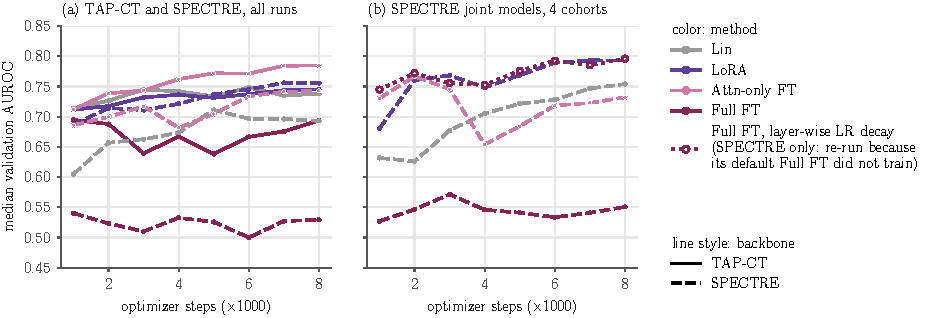
\includegraphics[width=\textwidth,height=0.74\textheight,keepaspectratio]{figures/fig_fullft_spectre.pdf}
\caption{Full fine-tuning on SPECTRE. (a) Median validation AUROC at each evaluation with the default settings, for TAP-CT and SPECTRE, over all runs of each method. (b) SPECTRE joint models on four cohorts, including Full FT with layer-wise learning-rate decay, the setting selected in Table~\ref{tab:fullftfix}, which gives the alternative settings on all three backbones; (b) shows SPECTRE, the one backbone on which Full FT failed.}
\label{fig:fullftspectre}
\end{figure}

\begin{table}[H]
\centering
\caption{Controls for two confounds of the main comparison: rsLoRA at a quarter of the learning rate, which matches LoRA's update scale at initialization, and fine-tuning the MLP instead of the attention weights. Held-out AUROC of the joint models, mean over the cohort's labels.}
\label{tab:controls}
\adjustbox{max width=\textwidth,max totalheight=0.8\textheight}{\footnotesize\begin{tabular}{lrrrrr}
\toprule
Cohort & LoRA & rsLoRA & rsLoRA (LR$/4$) & Attn-only FT & MLP-only FT \\
\midrule
\multicolumn{6}{@{}l}{\textit{TAP-CT}} \\
CVPR26 & 0.733 & 0.722 & 0.741 & 0.739 & 0.745 \\
FDG-PET/CT & 0.866 & 0.785 & 0.855 & 0.870 & 0.866 \\
RSNA23 trauma & 0.757 & 0.684 & 0.751 & 0.833 & 0.894 \\
RSNA22 C-spine & 0.714 & 0.601 & 0.611 & 0.712 & 0.627 \\
RSNA19 ICH & 0.906 & 0.869 & 0.901 & 0.915 & 0.907 \\
\multicolumn{6}{@{}l}{\textit{SPECTRE}} \\
CVPR26 & 0.716 & 0.690 & 0.739 & 0.740 & 0.681 \\
FDG-PET/CT & 0.901 & 0.900 & 0.908 & 0.906 & 0.814 \\
RSNA23 trauma & 0.846 & 0.850 & 0.834 & 0.803 & 0.838 \\
RSNA22 C-spine & 0.706 & 0.691 & 0.672 & 0.718 & 0.626 \\
\multicolumn{6}{@{}l}{\textit{Pillar-0}} \\
RSNA19 ICH & 0.912 & 0.918 & 0.920 & 0.912 & 0.912 \\
\bottomrule
\end{tabular}
}
\end{table}

\begin{table}[H]
\centering
\caption{Joint against compute-matched per-structure segmentation: held-out Dice, mean over the 15 structures, of per-structure models trained 1600 steps (matched) or 8000 steps, and of the 24\,000-step joint model on the same structures; the difference joint $-$ matched and the number of structures where it is positive.}
\label{tab:segcm}
\adjustbox{max width=\textwidth,max totalheight=0.8\textheight}{\footnotesize\begin{tabular}{llrrrrrc}
\toprule
 & & & \multicolumn{2}{c}{per-structure} & & \multicolumn{2}{c}{joint $-$ matched} \\
\cmidrule(lr){4-5}\cmidrule(lr){7-8}
Backbone & Method & \begin{tabular}[b]{@{}c@{}}Struct.\\finished\end{tabular} & matched & 8000 steps & joint & mean & $>0$ \\
\midrule
\multicolumn{8}{@{}l}{\textit{AMOS22 (15 structures)}} \\
TAP-CT & Dec & 15 & 0.763 & 0.793 & 0.708 & $-0.055$ & 11/15 \\
TAP-CT & LoRA & 15 & 0.617 & 0.767 & 0.739 & $+0.122$ & 14/15 \\
TAP-CT & Full FT & 15 & 0.766 & 0.805 & 0.681 & $-0.085$ & 12/15 \\
SPECTRE & Dec & 15 & 0.760 & 0.808 & 0.658 & $-0.101$ & 6/15 \\
SPECTRE & LoRA & 15 & 0.648 & 0.812 & 0.784 & $+0.136$ & 14/15 \\
SPECTRE & Full FT & 15 & 0.793 & 0.792 & 0.669 & $-0.123$ & 5/15 \\
\multicolumn{8}{@{}l}{\textit{TotalSegmentator (15 structures)}} \\
TAP-CT & Dec & 15 & 0.783 & 0.843 & 0.798 & $+0.015$ & 13/15 \\
TAP-CT & LoRA & 15 & 0.657 & 0.819 & 0.776 & $+0.119$ & 14/15 \\
TAP-CT & Full FT & 15 & 0.803 & 0.832 & 0.815 & $+0.012$ & 14/15 \\
SPECTRE & Dec & 15 & 0.806 & 0.848 & 0.770 & $-0.037$ & 6/15 \\
SPECTRE & LoRA & 15 & 0.691 & 0.848 & 0.733 & $+0.042$ & 11/15 \\
SPECTRE & Full FT & 15 & 0.819 & 0.838 & 0.795 & $-0.024$ & 10/15 \\
\bottomrule
\end{tabular}
}
\end{table}

\begin{table}[H]
\centering
\caption{From-scratch control: TAP-CT architecture with a randomly initialized encoder, trained as the Full FT joint model, next to Full FT and Dec, per dataset (held-out Dice, mean over structures).}
\label{tab:scratch}
\adjustbox{max width=\textwidth,max totalheight=0.8\textheight}{\footnotesize\begin{tabular}{@{}lccccc@{}}
\toprule
Dataset (structures) & From scratch & Dec & Full FT & Scratch $-$ Dec & Scratch $-$ Full FT \\
\midrule
AMOS22 (15) & 0.496 & 0.708 & 0.681 & -0.212 & -0.185 \\
KiTS23 (3) & 0.400 & 0.514 & 0.519 & -0.114 & -0.120 \\
LiTS (2) & 0.612 & 0.699 & 0.715 & -0.087 & -0.103 \\
MSD Pancreas (2) & 0.308 & 0.480 & 0.487 & -0.172 & -0.180 \\
TotalSegmentator (15) & 0.579 & 0.798 & 0.815 & -0.219 & -0.236 \\
\bottomrule
\end{tabular}
}
\end{table}

\clearpage
\section{Per-cohort, per-label and per-structure results}
\label{app:perlabel}
\begin{table}[H]
\centering
\caption{Classification: held-out AUROC, mean over the labels of each cohort (number of labels in brackets), per backbone, training mode and method. Within each row, \textbf{bold} is the best and \underline{underlined} the second-best method. A \colorbox{modebest}{shaded} cell marks the better of per-task and joint training for that method, backbone and cohort. SPECTRE Full FT did not train with the default setting (Section~\ref{sec:clsres}).}
\label{tab:cls}
\adjustbox{max width=\textwidth,max totalheight=0.8\textheight}{\footnotesize\setlength{\tabcolsep}{3pt}
\begin{tabular}{lllccccccccccc}
\toprule
Cohort (labels) & Backbone & Mode & Lin & Attn & LoRA & LoRA$_{\text{late}}$ & \begin{tabular}[b]{@{}c@{}}LoRA+\\ABMIL\end{tabular} & DoRA & rsLoRA & \begin{tabular}[b]{@{}c@{}}Lin$\to$\\LoRA\end{tabular} & \begin{tabular}[b]{@{}c@{}}Attn$\to$\\LoRA\end{tabular} & \begin{tabular}[b]{@{}c@{}}Attn-only\\FT\end{tabular} & \begin{tabular}[b]{@{}c@{}}Full\\FT\end{tabular} \\
\midrule
CVPR26 (17) & TAP-CT & per-task & 0.677 & 0.718 & \underline{0.732} & 0.704 & 0.728 & 0.717 & \cellcolor{modebest}0.724 & \cellcolor{modebest}0.697 & 0.707 & \cellcolor{modebest}\textbf{0.744} & 0.720 \\
 &  & joint & \cellcolor{modebest}0.707 & \cellcolor{modebest}0.720 & \cellcolor{modebest}0.733 & \cellcolor{modebest}0.726 & \cellcolor{modebest}0.729 & \cellcolor{modebest}0.733 & 0.722 & 0.695 & \cellcolor{modebest}0.708 & \underline{0.739} & \cellcolor{modebest}\textbf{0.744} \\
\addlinespace[2pt]
CVPR26 (17) & SPECTRE & per-task & \cellcolor{modebest}0.736 & 0.725 & \cellcolor{modebest}0.769 & \cellcolor{modebest}0.769 & \cellcolor{modebest}\underline{0.776} & \cellcolor{modebest}0.766 & \cellcolor{modebest}0.768 & \cellcolor{modebest}0.769 & \cellcolor{modebest}0.765 & \cellcolor{modebest}\textbf{0.778} & \cellcolor{modebest}0.627 \\
 &  & joint & 0.702 & \cellcolor{modebest}0.738 & 0.716 & 0.731 & \textbf{0.747} & 0.731 & 0.690 & \underline{0.744} & 0.728 & 0.740 & 0.575 \\
\addlinespace[2pt]
FDG-PET/CT (4) & TAP-CT & per-task & \cellcolor{modebest}0.863 & 0.836 & 0.852 & \cellcolor{modebest}\textbf{0.868} & 0.839 & 0.847 & \cellcolor{modebest}0.817 & \cellcolor{modebest}\underline{0.866} & 0.856 & 0.832 & \cellcolor{modebest}0.769 \\
 &  & joint & 0.858 & \cellcolor{modebest}0.860 & \cellcolor{modebest}\underline{0.866} & 0.864 & \cellcolor{modebest}0.849 & \cellcolor{modebest}0.858 & 0.785 & 0.860 & \cellcolor{modebest}0.862 & \cellcolor{modebest}\textbf{0.870} & 0.608 \\
\addlinespace[2pt]
FDG-PET/CT (4) & SPECTRE & per-task & 0.857 & 0.862 & 0.882 & 0.879 & 0.874 & \textbf{0.892} & 0.872 & \cellcolor{modebest}\underline{0.887} & 0.867 & 0.848 & 0.617 \\
 &  & joint & \cellcolor{modebest}0.884 & \cellcolor{modebest}0.880 & \cellcolor{modebest}\underline{0.901} & \cellcolor{modebest}0.888 & \cellcolor{modebest}0.889 & \cellcolor{modebest}0.900 & \cellcolor{modebest}0.900 & 0.884 & \cellcolor{modebest}0.884 & \cellcolor{modebest}\textbf{0.906} & \cellcolor{modebest}0.673 \\
\addlinespace[2pt]
RSNA22 C-spine (8) & TAP-CT & per-task & 0.619 & \cellcolor{modebest}0.625 & 0.623 & 0.608 & 0.613 & \underline{0.641} & \cellcolor{modebest}0.635 & 0.606 & \cellcolor{modebest}0.629 & \textbf{0.660} & 0.637 \\
 &  & joint & \cellcolor{modebest}0.626 & 0.624 & \cellcolor{modebest}\underline{0.714} & \cellcolor{modebest}0.706 & \cellcolor{modebest}0.713 & \cellcolor{modebest}0.680 & 0.601 & \cellcolor{modebest}0.624 & 0.620 & \cellcolor{modebest}0.712 & \cellcolor{modebest}\textbf{0.732} \\
\addlinespace[2pt]
RSNA22 C-spine (8) & SPECTRE & per-task & 0.579 & 0.591 & 0.635 & \cellcolor{modebest}\textbf{0.654} & \underline{0.644} & 0.619 & 0.638 & 0.615 & 0.591 & 0.635 & \cellcolor{modebest}0.566 \\
 &  & joint & \cellcolor{modebest}0.629 & \cellcolor{modebest}0.601 & \cellcolor{modebest}0.706 & 0.644 & \cellcolor{modebest}\textbf{0.730} & \cellcolor{modebest}0.692 & \cellcolor{modebest}0.691 & \cellcolor{modebest}0.670 & \cellcolor{modebest}0.611 & \cellcolor{modebest}\underline{0.718} & 0.554 \\
\addlinespace[2pt]
RSNA23 trauma (4) & TAP-CT & per-task & 0.737 & 0.718 & 0.739 & \cellcolor{modebest}0.756 & 0.703 & 0.752 & \cellcolor{modebest}0.725 & 0.738 & 0.716 & \cellcolor{modebest}\textbf{0.859} & \underline{0.775} \\
 &  & joint & \cellcolor{modebest}0.739 & \cellcolor{modebest}0.738 & \cellcolor{modebest}0.757 & 0.744 & \cellcolor{modebest}0.758 & \cellcolor{modebest}0.768 & 0.684 & \cellcolor{modebest}0.746 & \cellcolor{modebest}0.758 & \underline{0.833} & \cellcolor{modebest}\textbf{0.881} \\
\addlinespace[2pt]
RSNA23 trauma (4) & SPECTRE & per-task & \cellcolor{modebest}0.791 & 0.778 & 0.824 & 0.832 & \textbf{0.852} & \cellcolor{modebest}\underline{0.842} & 0.836 & 0.825 & 0.798 & 0.772 & 0.624 \\
 &  & joint & 0.789 & \cellcolor{modebest}0.788 & \cellcolor{modebest}0.846 & \cellcolor{modebest}0.835 & \cellcolor{modebest}\textbf{0.859} & 0.838 & \cellcolor{modebest}\underline{0.850} & \cellcolor{modebest}0.827 & \cellcolor{modebest}0.810 & \cellcolor{modebest}0.803 & \cellcolor{modebest}0.654 \\
\addlinespace[2pt]
RSNA19 ICH (6) & TAP-CT & per-task & 0.870 & 0.873 & 0.894 & 0.894 & \cellcolor{modebest}0.891 & \underline{0.897} & \cellcolor{modebest}0.870 & \cellcolor{modebest}0.877 & \cellcolor{modebest}0.878 & \textbf{0.911} & \cellcolor{modebest}0.888 \\
 &  & joint & \cellcolor{modebest}0.871 & \cellcolor{modebest}0.877 & \cellcolor{modebest}\underline{0.906} & \cellcolor{modebest}0.895 & 0.886 & 0.897 & 0.869 & 0.868 & 0.876 & \cellcolor{modebest}\textbf{0.915} & 0.854 \\
\addlinespace[2pt]
RSNA19 ICH (6) & Pillar-0 & per-task & 0.886 & 0.884 & \cellcolor{modebest}\underline{0.929} & \cellcolor{modebest}0.914 & 0.902 & \cellcolor{modebest}\textbf{0.931} & \cellcolor{modebest}0.920 & \cellcolor{modebest}0.912 & \cellcolor{modebest}0.903 & \cellcolor{modebest}\textbf{0.931} & \cellcolor{modebest}0.904 \\
 &  & joint & \cellcolor{modebest}0.888 & \cellcolor{modebest}0.888 & 0.912 & 0.892 & \cellcolor{modebest}\textbf{0.925} & 0.912 & \underline{0.918} & 0.905 & 0.898 & 0.912 & 0.878 \\
\addlinespace[2pt]
\bottomrule
\end{tabular}
}
\end{table}
\begin{table}[H]
\centering
\caption{Segmentation: held-out Dice, mean over the structures of each dataset (number of structures in brackets), per backbone, training mode and method; -- marks methods not run per structure on TotalSegmentator. Within each row, \textbf{bold} is the best and \underline{underlined} the second-best method. A \colorbox{modebest}{shaded} cell marks the better of per-structure and joint training for that method, backbone and dataset. The AMOS22 and TotalSegmentator joint models train 24\,000 steps.}
\label{tab:seg}
\adjustbox{max width=\textwidth,max totalheight=0.8\textheight}{\footnotesize\begin{tabular}{lllccccccc}
\toprule
Dataset (structures) & Backbone & Mode & Lin & Dec & LoRA & LoRA$_{\text{late}}$ & DoRA & Full FT & Dec$\to$LoRA \\
\midrule
AMOS22 (15) & TAP-CT & per-task & \cellcolor{modebest}0.658 & \cellcolor{modebest}\underline{0.793} & \cellcolor{modebest}0.767 & \cellcolor{modebest}0.764 & \cellcolor{modebest}0.761 & \cellcolor{modebest}\textbf{0.805} & \cellcolor{modebest}0.791 \\
 &  & joint & 0.646 & \underline{0.708} & \textbf{0.739} & 0.698 & \underline{0.708} & 0.681 & 0.656 \\
\addlinespace[2pt]
AMOS22 (15) & SPECTRE & per-task & \cellcolor{modebest}0.683 & \cellcolor{modebest}0.808 & \cellcolor{modebest}\underline{0.812} & \cellcolor{modebest}0.806 & \cellcolor{modebest}\textbf{0.814} & \cellcolor{modebest}0.792 & \cellcolor{modebest}\textbf{0.814} \\
 &  & joint & 0.682 & 0.658 & \textbf{0.784} & 0.764 & \underline{0.775} & 0.669 & 0.664 \\
\addlinespace[2pt]
KiTS23 (3) & TAP-CT & per-task & \cellcolor{modebest}0.531 & \cellcolor{modebest}0.584 & 0.563 & \cellcolor{modebest}0.567 & \cellcolor{modebest}0.563 & \cellcolor{modebest}\textbf{0.588} & \cellcolor{modebest}\underline{0.587} \\
 &  & joint & 0.430 & 0.514 & \cellcolor{modebest}\textbf{0.582} & 0.556 & \underline{0.560} & 0.519 & 0.500 \\
\addlinespace[2pt]
KiTS23 (3) & SPECTRE & per-task & \cellcolor{modebest}0.583 & \cellcolor{modebest}0.599 & \cellcolor{modebest}0.613 & \cellcolor{modebest}\underline{0.617} & \cellcolor{modebest}\textbf{0.622} & \cellcolor{modebest}0.528 & \cellcolor{modebest}0.603 \\
 &  & joint & 0.530 & 0.572 & \underline{0.588} & \underline{0.588} & \textbf{0.593} & 0.519 & 0.570 \\
\addlinespace[2pt]
LiTS (2) & TAP-CT & per-task & \cellcolor{modebest}0.659 & \cellcolor{modebest}0.709 & \cellcolor{modebest}\textbf{0.716} & 0.709 & \cellcolor{modebest}\underline{0.714} & 0.710 & \cellcolor{modebest}\underline{0.714} \\
 &  & joint & 0.656 & 0.699 & \underline{0.715} & \cellcolor{modebest}\textbf{0.721} & 0.692 & \cellcolor{modebest}\underline{0.715} & 0.703 \\
\addlinespace[2pt]
LiTS (2) & SPECTRE & per-task & 0.688 & \underline{0.741} & \cellcolor{modebest}\textbf{0.756} & 0.723 & \cellcolor{modebest}\textbf{0.756} & \cellcolor{modebest}0.739 & 0.729 \\
 &  & joint & \cellcolor{modebest}0.696 & \cellcolor{modebest}0.742 & \textbf{0.753} & \cellcolor{modebest}0.736 & \underline{0.743} & 0.713 & \cellcolor{modebest}\underline{0.743} \\
\addlinespace[2pt]
MSD Pancreas (2) & TAP-CT & per-task & \cellcolor{modebest}0.427 & \cellcolor{modebest}0.491 & \underline{0.504} & \cellcolor{modebest}0.501 & \cellcolor{modebest}0.502 & \cellcolor{modebest}\textbf{0.512} & \cellcolor{modebest}0.495 \\
 &  & joint & 0.334 & 0.480 & \cellcolor{modebest}\textbf{0.505} & 0.492 & \underline{0.493} & 0.487 & 0.468 \\
\addlinespace[2pt]
MSD Pancreas (2) & SPECTRE & per-task & \cellcolor{modebest}0.475 & \cellcolor{modebest}0.516 & \cellcolor{modebest}\textbf{0.563} & \cellcolor{modebest}0.538 & \cellcolor{modebest}\underline{0.557} & 0.516 & 0.518 \\
 &  & joint & 0.459 & 0.514 & \textbf{0.550} & 0.529 & \textbf{0.550} & \cellcolor{modebest}\underline{0.530} & \cellcolor{modebest}0.520 \\
\addlinespace[2pt]
TotalSegmentator (15) & TAP-CT & per-task & \cellcolor{modebest}0.747 & \cellcolor{modebest}\textbf{0.843} & \cellcolor{modebest}0.819 & -- & -- & \cellcolor{modebest}\underline{0.832} & -- \\
 &  & joint & 0.740 & \underline{0.798} & 0.776 & 0.776 & 0.776 & \textbf{0.815} & 0.790 \\
\addlinespace[2pt]
TotalSegmentator (15) & SPECTRE & per-task & \cellcolor{modebest}0.731 & \cellcolor{modebest}\textbf{0.848} & \cellcolor{modebest}\textbf{0.848} & -- & -- & \cellcolor{modebest}\underline{0.838} & -- \\
 &  & joint & 0.722 & 0.770 & 0.733 & 0.752 & 0.736 & \textbf{0.795} & \underline{0.772} \\
\addlinespace[2pt]
\bottomrule
\end{tabular}
}
\end{table}

\begin{table}[H]
\centering
\caption{Held-out AUROC as in Table~\ref{tab:cls}, with the longer CVPR26 joint schedule (26\,000 steps) as an extra row. \textbf{Bold}: best, \underline{underlined}: second best of the row; \colorbox{modebest}{shaded}: the better of per-task and joint training (8000 steps).}
\label{tab:ladder}
\adjustbox{max width=\textwidth,max totalheight=0.8\textheight}{\footnotesize\begin{tabular}{lllccccccccccc}
\toprule
Cohort & Backbone & Mode (labels) & Lin & Attn & LoRA & LoRA$_{\text{late}}$ & LoRA+ABMIL & DoRA & rsLoRA & Lin$\to$LoRA & Attn$\to$LoRA & Attn-only FT & Full FT \\
\midrule
CVPR26 & TAP-CT & per-task (17) & 0.677 & 0.718 & \underline{0.732} & 0.704 & 0.728 & 0.717 & \cellcolor{modebest}0.724 & \cellcolor{modebest}0.697 & 0.707 & \cellcolor{modebest}\textbf{0.744} & 0.720 \\
CVPR26 & TAP-CT & joint (17) & \cellcolor{modebest}0.707 & \cellcolor{modebest}0.720 & \cellcolor{modebest}0.733 & \cellcolor{modebest}0.726 & \cellcolor{modebest}0.729 & \cellcolor{modebest}0.733 & 0.722 & 0.695 & \cellcolor{modebest}0.708 & \underline{0.739} & \cellcolor{modebest}\textbf{0.744} \\
CVPR26 & TAP-CT & joint (26\,000 steps) (17) & 0.693 & 0.722 & 0.692 & \underline{0.728} & 0.727 & 0.720 & 0.701 & 0.698 & 0.726 & \textbf{0.756} & 0.650 \\
\addlinespace[2pt]
CVPR26 & SPECTRE & per-task (17) & \cellcolor{modebest}0.736 & 0.725 & \cellcolor{modebest}0.769 & \cellcolor{modebest}0.769 & \cellcolor{modebest}\underline{0.776} & \cellcolor{modebest}0.766 & \cellcolor{modebest}0.768 & \cellcolor{modebest}0.769 & \cellcolor{modebest}0.765 & \cellcolor{modebest}\textbf{0.778} & \cellcolor{modebest}0.627 \\
CVPR26 & SPECTRE & joint (17) & 0.702 & \cellcolor{modebest}0.738 & 0.716 & 0.731 & \textbf{0.747} & 0.731 & 0.690 & \underline{0.744} & 0.728 & 0.740 & 0.575 \\
CVPR26 & SPECTRE & joint (26\,000 steps) (17) & 0.744 & 0.713 & 0.755 & \underline{0.762} & 0.760 & 0.752 & \textbf{0.763} & 0.746 & 0.758 & 0.756 & 0.574 \\
\addlinespace[2pt]
FDG-PET/CT & TAP-CT & per-task (4) & \cellcolor{modebest}0.863 & 0.836 & 0.852 & \cellcolor{modebest}\textbf{0.868} & 0.839 & 0.847 & \cellcolor{modebest}0.817 & \cellcolor{modebest}\underline{0.866} & 0.856 & 0.832 & \cellcolor{modebest}0.769 \\
FDG-PET/CT & TAP-CT & joint (4) & 0.858 & \cellcolor{modebest}0.860 & \cellcolor{modebest}\underline{0.866} & 0.864 & \cellcolor{modebest}0.849 & \cellcolor{modebest}0.858 & 0.785 & 0.860 & \cellcolor{modebest}0.862 & \cellcolor{modebest}\textbf{0.870} & 0.608 \\
\addlinespace[2pt]
FDG-PET/CT & SPECTRE & per-task (4) & 0.857 & 0.862 & 0.882 & 0.879 & 0.874 & \textbf{0.892} & 0.872 & \cellcolor{modebest}\underline{0.887} & 0.867 & 0.848 & 0.617 \\
FDG-PET/CT & SPECTRE & joint (4) & \cellcolor{modebest}0.884 & \cellcolor{modebest}0.880 & \cellcolor{modebest}\underline{0.901} & \cellcolor{modebest}0.888 & \cellcolor{modebest}0.889 & \cellcolor{modebest}0.900 & \cellcolor{modebest}0.900 & 0.884 & \cellcolor{modebest}0.884 & \cellcolor{modebest}\textbf{0.906} & \cellcolor{modebest}0.673 \\
\addlinespace[2pt]
RSNA22 C-spine & TAP-CT & per-task (8) & 0.619 & \cellcolor{modebest}0.625 & 0.623 & 0.608 & 0.613 & \underline{0.641} & \cellcolor{modebest}0.635 & 0.606 & \cellcolor{modebest}0.629 & \textbf{0.660} & 0.637 \\
RSNA22 C-spine & TAP-CT & joint (8) & \cellcolor{modebest}0.626 & 0.624 & \cellcolor{modebest}\underline{0.714} & \cellcolor{modebest}0.706 & \cellcolor{modebest}0.713 & \cellcolor{modebest}0.680 & 0.601 & \cellcolor{modebest}0.624 & 0.620 & \cellcolor{modebest}0.712 & \cellcolor{modebest}\textbf{0.732} \\
\addlinespace[2pt]
RSNA22 C-spine & SPECTRE & per-task (8) & 0.579 & 0.591 & 0.635 & \cellcolor{modebest}\textbf{0.654} & \underline{0.644} & 0.619 & 0.638 & 0.615 & 0.591 & 0.635 & \cellcolor{modebest}0.566 \\
RSNA22 C-spine & SPECTRE & joint (8) & \cellcolor{modebest}0.629 & \cellcolor{modebest}0.601 & \cellcolor{modebest}0.706 & 0.644 & \cellcolor{modebest}\textbf{0.730} & \cellcolor{modebest}0.692 & \cellcolor{modebest}0.691 & \cellcolor{modebest}0.670 & \cellcolor{modebest}0.611 & \cellcolor{modebest}\underline{0.718} & 0.554 \\
\addlinespace[2pt]
RSNA23 trauma & TAP-CT & per-task (4) & 0.737 & 0.718 & 0.739 & \cellcolor{modebest}0.756 & 0.703 & 0.752 & \cellcolor{modebest}0.725 & 0.738 & 0.716 & \cellcolor{modebest}\textbf{0.859} & \underline{0.775} \\
RSNA23 trauma & TAP-CT & joint (4) & \cellcolor{modebest}0.739 & \cellcolor{modebest}0.738 & \cellcolor{modebest}0.757 & 0.744 & \cellcolor{modebest}0.758 & \cellcolor{modebest}0.768 & 0.684 & \cellcolor{modebest}0.746 & \cellcolor{modebest}0.758 & \underline{0.833} & \cellcolor{modebest}\textbf{0.881} \\
\addlinespace[2pt]
RSNA23 trauma & SPECTRE & per-task (4) & \cellcolor{modebest}0.791 & 0.778 & 0.824 & 0.832 & \textbf{0.852} & \cellcolor{modebest}\underline{0.842} & 0.836 & 0.825 & 0.798 & 0.772 & 0.624 \\
RSNA23 trauma & SPECTRE & joint (4) & 0.789 & \cellcolor{modebest}0.788 & \cellcolor{modebest}0.846 & \cellcolor{modebest}0.835 & \cellcolor{modebest}\textbf{0.859} & 0.838 & \cellcolor{modebest}\underline{0.850} & \cellcolor{modebest}0.827 & \cellcolor{modebest}0.810 & \cellcolor{modebest}0.803 & \cellcolor{modebest}0.654 \\
\addlinespace[2pt]
RSNA19 ICH & TAP-CT & per-task (6) & 0.870 & 0.873 & 0.894 & 0.894 & \cellcolor{modebest}0.891 & \underline{0.897} & \cellcolor{modebest}0.870 & \cellcolor{modebest}0.877 & \cellcolor{modebest}0.878 & \textbf{0.911} & \cellcolor{modebest}0.888 \\
RSNA19 ICH & TAP-CT & joint (6) & \cellcolor{modebest}0.871 & \cellcolor{modebest}0.877 & \cellcolor{modebest}\underline{0.906} & \cellcolor{modebest}0.895 & 0.886 & 0.897 & 0.869 & 0.868 & 0.876 & \cellcolor{modebest}\textbf{0.915} & 0.854 \\
\addlinespace[2pt]
RSNA19 ICH & Pillar-0 & per-task (6) & 0.886 & 0.884 & \cellcolor{modebest}\underline{0.929} & \cellcolor{modebest}0.914 & 0.902 & \cellcolor{modebest}\textbf{0.931} & \cellcolor{modebest}0.920 & \cellcolor{modebest}0.912 & \cellcolor{modebest}0.903 & \cellcolor{modebest}\textbf{0.931} & \cellcolor{modebest}0.904 \\
RSNA19 ICH & Pillar-0 & joint (6) & \cellcolor{modebest}0.888 & \cellcolor{modebest}0.888 & 0.912 & 0.892 & \cellcolor{modebest}\textbf{0.925} & 0.912 & \underline{0.918} & 0.905 & 0.898 & 0.912 & 0.878 \\
\addlinespace[2pt]
\bottomrule
\end{tabular}
}
\end{table}

\clearpage
\begin{center}\begin{minipage}{\textwidth}\centering\footnotesize\textit{CVPR26, TAP-CT}\\[2pt]\adjustbox{max width=\textwidth}{\begin{tabular}{lccccccccccc}
\toprule
Label & Lin & Attn & LoRA & LoRA$_{\text{late}}$ & LoRA+ABMIL & DoRA & rsLoRA & Lin$\to$LoRA & Attn$\to$LoRA & Attn-only FT & Full FT \\
\midrule
\multicolumn{12}{l}{\textit{TAP-CT, per-task}} \\
adrenal\_hyperplasia & 0.80 [0.62,0.95] & 0.84 [0.68,0.97] & 0.80 [0.62,0.96] & 0.79 [0.62,0.95] & 0.81 [0.64,0.95] & 0.77 [0.59,0.92] & 0.79 [0.60,0.94] & 0.80 [0.62,0.95] & 0.82 [0.67,0.95] & 0.84 [0.68,0.97] & 0.87 [0.72,0.98] \\
ascites & 0.78 [0.60,0.92] & 0.84 [0.67,0.97] & 0.77 [0.59,0.92] & 0.74 [0.55,0.90] & 0.78 [0.61,0.92] & 0.71 [0.50,0.87] & 0.77 [0.60,0.93] & 0.76 [0.58,0.92] & 0.75 [0.56,0.92] & 0.68 [0.47,0.85] & 0.82 [0.66,0.95] \\
atherosclerosis & 0.75 [0.57,0.90] & 0.87 [0.73,0.97] & 0.89 [0.76,0.97] & 0.83 [0.68,0.96] & 0.83 [0.68,0.95] & 0.84 [0.68,0.96] & 0.86 [0.71,0.97] & 0.75 [0.56,0.90] & 0.86 [0.71,0.97] & 0.81 [0.64,0.93] & 0.88 [0.74,0.97] \\
cholecystitis & 0.73 [0.56,0.88] & 0.78 [0.62,0.92] & 0.74 [0.55,0.90] & 0.69 [0.49,0.85] & 0.73 [0.54,0.89] & 0.75 [0.60,0.90] & 0.74 [0.56,0.89] & 0.75 [0.56,0.91] & 0.72 [0.56,0.88] & 0.77 [0.60,0.91] & 0.74 [0.57,0.89] \\
colorectal\_cancer & 0.56 [0.33,0.77] & 0.65 [0.44,0.85] & 0.65 [0.43,0.88] & 0.65 [0.43,0.85] & 0.67 [0.43,0.86] & 0.63 [0.40,0.84] & 0.62 [0.38,0.84] & 0.60 [0.37,0.84] & 0.64 [0.42,0.85] & 0.70 [0.48,0.88] & 0.62 [0.41,0.82] \\
fatty\_liver & 0.87 [0.75,0.97] & 0.92 [0.82,0.99] & 0.95 [0.88,1.00] & 0.95 [0.86,1.00] & 0.95 [0.88,1.00] & 0.94 [0.85,0.99] & 0.99 [0.97,1.00] & 0.90 [0.78,0.99] & 0.92 [0.82,0.98] & 0.99 [0.97,1.00] & 0.98 [0.94,1.00] \\
gallstone & 0.60 [0.46,0.74] & 0.65 [0.49,0.78] & 0.66 [0.52,0.80] & 0.64 [0.50,0.78] & 0.68 [0.54,0.81] & 0.68 [0.53,0.82] & 0.60 [0.46,0.74] & 0.61 [0.46,0.75] & 0.69 [0.55,0.82] & 0.65 [0.51,0.78] & 0.69 [0.56,0.82] \\
hydronephrosis & 0.86 [0.71,0.97] & 0.82 [0.64,0.95] & 0.90 [0.78,0.98] & 0.86 [0.70,0.97] & 0.86 [0.71,0.96] & 0.85 [0.70,0.96] & 0.78 [0.61,0.92] & 0.87 [0.71,0.97] & 0.90 [0.78,0.98] & 0.86 [0.71,0.97] & 0.67 [0.47,0.85] \\
kidney\_stone & 0.62 [0.49,0.75] & 0.69 [0.57,0.80] & 0.63 [0.50,0.75] & 0.65 [0.52,0.77] & 0.64 [0.50,0.76] & 0.62 [0.51,0.74] & 0.70 [0.58,0.81] & 0.70 [0.57,0.81] & 0.71 [0.59,0.83] & 0.70 [0.58,0.80] & 0.67 [0.56,0.79] \\
liver\_calcifications & 0.44 [0.25,0.63] & 0.37 [0.20,0.56] & 0.49 [0.30,0.69] & 0.44 [0.26,0.63] & 0.47 [0.28,0.67] & 0.51 [0.32,0.69] & 0.51 [0.31,0.71] & 0.43 [0.26,0.63] & 0.39 [0.22,0.59] & 0.58 [0.38,0.75] & 0.57 [0.40,0.75] \\
liver\_cyst & 0.64 [0.54,0.74] & 0.67 [0.57,0.76] & 0.67 [0.56,0.77] & 0.64 [0.54,0.74] & 0.65 [0.54,0.75] & 0.62 [0.53,0.73] & 0.68 [0.57,0.77] & 0.66 [0.57,0.76] & 0.64 [0.55,0.73] & 0.69 [0.60,0.78] & 0.66 [0.55,0.75] \\
liver\_lesion & 0.57 [0.42,0.72] & 0.64 [0.48,0.77] & 0.71 [0.57,0.83] & 0.69 [0.56,0.81] & 0.61 [0.47,0.75] & 0.66 [0.52,0.79] & 0.65 [0.51,0.78] & 0.59 [0.45,0.73] & 0.64 [0.51,0.77] & 0.66 [0.52,0.80] & 0.70 [0.57,0.82] \\
lymphadenopathy & 0.60 [0.41,0.78] & 0.73 [0.57,0.88] & 0.64 [0.48,0.81] & 0.67 [0.48,0.85] & 0.76 [0.61,0.91] & 0.73 [0.55,0.88] & 0.66 [0.46,0.82] & 0.69 [0.51,0.85] & 0.70 [0.52,0.85] & 0.76 [0.60,0.90] & 0.54 [0.36,0.72] \\
renal\_cyst & 0.66 [0.57,0.75] & 0.64 [0.55,0.73] & 0.67 [0.58,0.76] & 0.69 [0.60,0.77] & 0.65 [0.56,0.74] & 0.64 [0.55,0.73] & 0.69 [0.60,0.77] & 0.64 [0.55,0.73] & 0.64 [0.54,0.73] & 0.66 [0.57,0.75] & 0.67 [0.57,0.75] \\
splenomegaly & 0.68 [0.52,0.85] & 0.75 [0.59,0.88] & 0.71 [0.54,0.85] & 0.72 [0.57,0.86] & 0.71 [0.55,0.88] & 0.71 [0.54,0.87] & 0.73 [0.57,0.87] & 0.70 [0.53,0.87] & 0.71 [0.54,0.86] & 0.72 [0.55,0.87] & 0.71 [0.55,0.86] \\
covid & 0.81 [0.65,0.96] & 0.76 [0.58,0.91] & 0.97 [0.92,1.00] & 0.75 [0.57,0.91] & 0.99 [0.96,1.00] & 0.99 [0.95,1.00] & 0.98 [0.93,1.00] & 0.84 [0.68,0.96] & 0.77 [0.60,0.93] & 1.00 [0.98,1.00] & 0.92 [0.78,1.00] \\
lung\_nodule\_malignancy & 0.53 [0.42,0.63] & 0.57 [0.45,0.69] & 0.59 [0.47,0.71] & 0.56 [0.46,0.67] & 0.57 [0.45,0.68] & 0.55 [0.43,0.66] & 0.57 [0.46,0.69] & 0.56 [0.45,0.67] & 0.50 [0.39,0.62] & 0.59 [0.48,0.70] & 0.55 [0.43,0.66] \\
\bottomrule
\end{tabular}
}\end{minipage}\end{center}
\begin{center}\begin{minipage}{\textwidth}\centering\footnotesize\textit{CVPR26, TAP-CT}\\[2pt]\adjustbox{max width=\textwidth}{\begin{tabular}{lccccccccccc}
\toprule
Label & Lin & Attn & LoRA & LoRA$_{\text{late}}$ & LoRA+ABMIL & DoRA & rsLoRA & Lin$\to$LoRA & Attn$\to$LoRA & Attn-only FT & Full FT \\
\midrule
\multicolumn{12}{l}{\textit{TAP-CT, joint}} \\
adrenal\_hyperplasia & 0.84 [0.69,0.96] & 0.83 [0.67,0.97] & 0.85 [0.69,0.98] & 0.84 [0.68,0.96] & 0.87 [0.74,0.97] & 0.82 [0.63,0.95] & 0.82 [0.64,0.94] & 0.87 [0.74,0.97] & 0.83 [0.68,0.95] & 0.80 [0.63,0.95] & 0.87 [0.71,0.98] \\
ascites & 0.77 [0.58,0.93] & 0.80 [0.62,0.94] & 0.84 [0.69,0.97] & 0.80 [0.61,0.95] & 0.75 [0.56,0.91] & 0.81 [0.65,0.96] & 0.81 [0.65,0.95] & 0.77 [0.58,0.91] & 0.68 [0.47,0.85] & 0.89 [0.76,0.98] & 0.81 [0.64,0.94] \\
atherosclerosis & 0.83 [0.70,0.95] & 0.81 [0.64,0.93] & 0.87 [0.73,0.97] & 0.83 [0.69,0.95] & 0.81 [0.64,0.94] & 0.81 [0.64,0.94] & 0.85 [0.70,0.96] & 0.82 [0.65,0.94] & 0.78 [0.60,0.91] & 0.83 [0.66,0.97] & 0.84 [0.67,0.96] \\
cholecystitis & 0.76 [0.57,0.91] & 0.70 [0.52,0.87] & 0.71 [0.54,0.87] & 0.77 [0.58,0.92] & 0.76 [0.58,0.89] & 0.73 [0.56,0.88] & 0.73 [0.53,0.88] & 0.71 [0.53,0.88] & 0.71 [0.55,0.87] & 0.72 [0.56,0.87] & 0.72 [0.55,0.88] \\
colorectal\_cancer & 0.62 [0.39,0.83] & 0.64 [0.40,0.86] & 0.70 [0.46,0.89] & 0.67 [0.43,0.87] & 0.67 [0.44,0.88] & 0.66 [0.41,0.88] & 0.67 [0.43,0.86] & 0.61 [0.38,0.81] & 0.68 [0.44,0.88] & 0.67 [0.44,0.86] & 0.64 [0.39,0.83] \\
fatty\_liver & 0.84 [0.69,0.96] & 0.80 [0.62,0.94] & 0.78 [0.60,0.91] & 0.76 [0.57,0.90] & 0.82 [0.67,0.93] & 0.79 [0.62,0.94] & 0.78 [0.61,0.92] & 0.82 [0.67,0.94] & 0.75 [0.58,0.91] & 0.81 [0.65,0.93] & 0.88 [0.75,0.97] \\
gallstone & 0.67 [0.53,0.79] & 0.66 [0.52,0.80] & 0.65 [0.50,0.78] & 0.63 [0.48,0.77] & 0.66 [0.51,0.79] & 0.67 [0.53,0.81] & 0.66 [0.52,0.79] & 0.67 [0.52,0.80] & 0.66 [0.51,0.79] & 0.68 [0.54,0.80] & 0.67 [0.53,0.80] \\
hydronephrosis & 0.86 [0.71,0.98] & 0.83 [0.69,0.95] & 0.79 [0.63,0.93] & 0.77 [0.59,0.92] & 0.81 [0.65,0.94] & 0.82 [0.65,0.96] & 0.70 [0.49,0.88] & 0.83 [0.67,0.96] & 0.79 [0.61,0.93] & 0.78 [0.58,0.94] & 0.76 [0.58,0.91] \\
kidney\_stone & 0.74 [0.62,0.84] & 0.69 [0.56,0.80] & 0.70 [0.59,0.82] & 0.71 [0.58,0.82] & 0.71 [0.58,0.81] & 0.67 [0.56,0.79] & 0.63 [0.50,0.74] & 0.69 [0.58,0.81] & 0.68 [0.56,0.81] & 0.63 [0.50,0.74] & 0.71 [0.60,0.82] \\
liver\_calcifications & 0.43 [0.25,0.62] & 0.51 [0.32,0.71] & 0.46 [0.26,0.65] & 0.51 [0.32,0.72] & 0.50 [0.33,0.71] & 0.52 [0.34,0.72] & 0.47 [0.29,0.68] & 0.40 [0.22,0.58] & 0.51 [0.33,0.71] & 0.54 [0.34,0.76] & 0.58 [0.38,0.77] \\
liver\_cyst & 0.63 [0.53,0.73] & 0.67 [0.57,0.76] & 0.65 [0.55,0.75] & 0.66 [0.56,0.75] & 0.66 [0.56,0.75] & 0.66 [0.56,0.76] & 0.65 [0.55,0.74] & 0.63 [0.52,0.72] & 0.63 [0.53,0.72] & 0.67 [0.57,0.77] & 0.67 [0.56,0.76] \\
liver\_lesion & 0.63 [0.48,0.77] & 0.71 [0.58,0.83] & 0.70 [0.56,0.81] & 0.69 [0.55,0.82] & 0.70 [0.57,0.82] & 0.68 [0.54,0.81] & 0.70 [0.56,0.82] & 0.66 [0.52,0.79] & 0.70 [0.56,0.82] & 0.69 [0.55,0.80] & 0.66 [0.52,0.79] \\
lymphadenopathy & 0.73 [0.55,0.88] & 0.77 [0.60,0.91] & 0.78 [0.61,0.92] & 0.74 [0.56,0.89] & 0.71 [0.55,0.86] & 0.75 [0.56,0.89] & 0.78 [0.61,0.92] & 0.73 [0.58,0.88] & 0.68 [0.51,0.85] & 0.74 [0.55,0.89] & 0.78 [0.59,0.93] \\
renal\_cyst & 0.60 [0.50,0.69] & 0.64 [0.54,0.72] & 0.66 [0.57,0.75] & 0.66 [0.57,0.75] & 0.68 [0.60,0.78] & 0.68 [0.60,0.76] & 0.66 [0.56,0.74] & 0.61 [0.52,0.70] & 0.65 [0.55,0.74] & 0.70 [0.61,0.79] & 0.67 [0.58,0.76] \\
splenomegaly & 0.72 [0.56,0.86] & 0.78 [0.63,0.91] & 0.86 [0.73,0.95] & 0.82 [0.66,0.95] & 0.80 [0.65,0.92] & 0.91 [0.81,0.98] & 0.87 [0.75,0.97] & 0.68 [0.52,0.84] & 0.78 [0.64,0.91] & 0.86 [0.74,0.96] & 0.84 [0.70,0.95] \\
covid & 0.83 [0.66,0.97] & 0.74 [0.56,0.89] & 0.83 [0.67,0.97] & 0.82 [0.64,0.96] & 0.84 [0.69,0.97] & 0.82 [0.65,0.96] & 0.86 [0.69,0.98] & 0.82 [0.65,0.95] & 0.84 [0.69,0.97] & 0.89 [0.75,1.00] & 0.93 [0.82,1.00] \\
lung\_nodule\_malignancy & 0.51 [0.39,0.63] & 0.67 [0.55,0.76] & 0.65 [0.53,0.75] & 0.67 [0.57,0.77] & 0.64 [0.53,0.74] & 0.65 [0.53,0.75] & 0.65 [0.55,0.75] & 0.48 [0.37,0.60] & 0.68 [0.58,0.78] & 0.66 [0.54,0.76] & 0.62 [0.51,0.73] \\
\bottomrule
\end{tabular}
}\end{minipage}\end{center}
\begin{center}\begin{minipage}{\textwidth}\centering\footnotesize\textit{CVPR26, TAP-CT}\\[2pt]\adjustbox{max width=\textwidth}{\begin{tabular}{lccccccccccc}
\toprule
Label & Lin & Attn & LoRA & LoRA$_{\text{late}}$ & LoRA+ABMIL & DoRA & rsLoRA & Lin$\to$LoRA & Attn$\to$LoRA & Attn-only FT & Full FT \\
\midrule
\multicolumn{12}{l}{\textit{TAP-CT, joint (26\,000 steps)}} \\
adrenal\_hyperplasia & 0.80 [0.61,0.94] & 0.76 [0.59,0.92] & 0.62 [0.42,0.80] & 0.80 [0.62,0.94] & 0.76 [0.59,0.92] & 0.81 [0.64,0.94] & 0.85 [0.70,0.97] & 0.81 [0.64,0.95] & 0.80 [0.62,0.95] & 0.88 [0.75,0.99] & 0.88 [0.74,0.98] \\
ascites & 0.79 [0.61,0.93] & 0.81 [0.63,0.94] & 0.82 [0.65,0.96] & 0.85 [0.68,0.97] & 0.77 [0.58,0.92] & 0.86 [0.69,1.00] & 0.82 [0.66,0.96] & 0.78 [0.59,0.93] & 0.72 [0.52,0.87] & 0.76 [0.59,0.91] & 0.62 [0.41,0.80] \\
atherosclerosis & 0.80 [0.61,0.93] & 0.82 [0.65,0.95] & 0.84 [0.69,0.96] & 0.82 [0.67,0.95] & 0.74 [0.54,0.90] & 0.77 [0.59,0.92] & 0.80 [0.63,0.93] & 0.79 [0.62,0.92] & 0.78 [0.60,0.92] & 0.85 [0.68,0.97] & 0.62 [0.42,0.81] \\
cholecystitis & 0.81 [0.64,0.94] & 0.70 [0.53,0.85] & 0.69 [0.50,0.83] & 0.71 [0.53,0.87] & 0.73 [0.57,0.88] & 0.71 [0.51,0.87] & 0.68 [0.50,0.84] & 0.87 [0.75,0.97] & 0.84 [0.70,0.94] & 0.73 [0.56,0.88] & 0.66 [0.48,0.83] \\
colorectal\_cancer & 0.60 [0.38,0.85] & 0.71 [0.49,0.91] & 0.59 [0.37,0.82] & 0.70 [0.48,0.91] & 0.61 [0.38,0.83] & 0.63 [0.40,0.85] & 0.71 [0.50,0.89] & 0.58 [0.36,0.82] & 0.72 [0.47,0.90] & 0.68 [0.46,0.88] & 0.58 [0.35,0.80] \\
fatty\_liver & 0.85 [0.71,0.97] & 0.85 [0.72,0.96] & 0.79 [0.62,0.93] & 0.85 [0.71,0.95] & 0.88 [0.75,0.98] & 0.80 [0.64,0.93] & 0.72 [0.54,0.88] & 0.86 [0.73,0.96] & 0.85 [0.70,0.96] & 0.90 [0.78,0.97] & 0.73 [0.56,0.88] \\
gallstone & 0.62 [0.47,0.76] & 0.62 [0.47,0.75] & 0.66 [0.51,0.80] & 0.62 [0.47,0.76] & 0.65 [0.51,0.80] & 0.68 [0.53,0.82] & 0.68 [0.55,0.81] & 0.65 [0.51,0.79] & 0.63 [0.48,0.77] & 0.66 [0.52,0.80] & 0.65 [0.52,0.79] \\
hydronephrosis & 0.83 [0.67,0.96] & 0.84 [0.69,0.95] & 0.76 [0.59,0.92] & 0.74 [0.55,0.90] & 0.79 [0.62,0.93] & 0.76 [0.57,0.91] & 0.69 [0.50,0.88] & 0.84 [0.68,0.95] & 0.80 [0.64,0.93] & 0.77 [0.57,0.93] & 0.70 [0.49,0.87] \\
kidney\_stone & 0.68 [0.55,0.79] & 0.72 [0.61,0.83] & 0.65 [0.53,0.77] & 0.67 [0.56,0.79] & 0.67 [0.55,0.79] & 0.65 [0.53,0.77] & 0.65 [0.53,0.77] & 0.69 [0.56,0.80] & 0.73 [0.61,0.83] & 0.67 [0.54,0.77] & 0.59 [0.46,0.72] \\
liver\_calcifications & 0.49 [0.30,0.69] & 0.43 [0.25,0.62] & 0.44 [0.25,0.63] & 0.54 [0.34,0.73] & 0.44 [0.24,0.62] & 0.52 [0.34,0.71] & 0.48 [0.30,0.67] & 0.39 [0.20,0.58] & 0.42 [0.24,0.63] & 0.52 [0.33,0.72] & 0.40 [0.22,0.58] \\
liver\_cyst & 0.65 [0.54,0.75] & 0.69 [0.59,0.78] & 0.63 [0.53,0.73] & 0.71 [0.61,0.80] & 0.72 [0.63,0.81] & 0.72 [0.63,0.81] & 0.63 [0.51,0.72] & 0.63 [0.52,0.72] & 0.68 [0.58,0.77] & 0.67 [0.57,0.76] & 0.59 [0.48,0.69] \\
liver\_lesion & 0.54 [0.39,0.68] & 0.71 [0.58,0.83] & 0.70 [0.56,0.82] & 0.66 [0.52,0.79] & 0.70 [0.57,0.82] & 0.70 [0.57,0.82] & 0.66 [0.52,0.79] & 0.60 [0.46,0.75] & 0.71 [0.58,0.82] & 0.70 [0.57,0.83] & 0.67 [0.54,0.80] \\
lymphadenopathy & 0.69 [0.51,0.86] & 0.73 [0.55,0.88] & 0.63 [0.45,0.79] & 0.74 [0.57,0.90] & 0.78 [0.60,0.93] & 0.78 [0.60,0.91] & 0.68 [0.48,0.84] & 0.69 [0.52,0.85] & 0.74 [0.56,0.89] & 0.77 [0.59,0.92] & 0.67 [0.47,0.83] \\
renal\_cyst & 0.61 [0.52,0.70] & 0.66 [0.57,0.75] & 0.63 [0.54,0.73] & 0.69 [0.59,0.77] & 0.72 [0.64,0.81] & 0.66 [0.56,0.74] & 0.68 [0.59,0.77] & 0.62 [0.53,0.72] & 0.65 [0.56,0.75] & 0.68 [0.59,0.77] & 0.58 [0.48,0.67] \\
splenomegaly & 0.73 [0.58,0.87] & 0.83 [0.69,0.93] & 0.87 [0.77,0.96] & 0.81 [0.65,0.93] & 0.81 [0.67,0.92] & 0.88 [0.76,0.97] & 0.75 [0.60,0.89] & 0.73 [0.56,0.88] & 0.79 [0.65,0.91] & 0.82 [0.67,0.93] & 0.76 [0.61,0.90] \\
covid & 0.78 [0.61,0.94] & 0.76 [0.59,0.91] & 0.81 [0.64,0.95] & 0.80 [0.61,0.94] & 0.94 [0.80,1.00] & 0.78 [0.59,0.95] & 0.85 [0.69,0.99] & 0.81 [0.66,0.94] & 0.82 [0.65,0.96] & 0.99 [0.96,1.00] & 0.79 [0.62,0.94] \\
lung\_nodule\_malignancy & 0.52 [0.40,0.64] & 0.64 [0.53,0.74] & 0.63 [0.52,0.74] & 0.68 [0.58,0.78] & 0.65 [0.54,0.75] & 0.53 [0.42,0.64] & 0.58 [0.47,0.69] & 0.53 [0.41,0.64] & 0.65 [0.54,0.76] & 0.78 [0.70,0.87] & 0.56 [0.45,0.68] \\
\bottomrule
\end{tabular}
}\end{minipage}\end{center}
\begin{center}\begin{minipage}{\textwidth}\centering\footnotesize\textit{CVPR26, SPECTRE}\\[2pt]\adjustbox{max width=\textwidth}{\begin{tabular}{lccccccccccc}
\toprule
Label & Lin & Attn & LoRA & LoRA$_{\text{late}}$ & LoRA+ABMIL & DoRA & rsLoRA & Lin$\to$LoRA & Attn$\to$LoRA & Attn-only FT & Full FT \\
\midrule
\multicolumn{12}{l}{\textit{SPECTRE, per-task}} \\
adrenal\_hyperplasia & 0.81 [0.64,0.93] & 0.52 [0.33,0.75] & 0.83 [0.66,0.94] & 0.80 [0.62,0.95] & 0.86 [0.71,0.96] & 0.59 [0.37,0.80] & 0.76 [0.58,0.91] & 0.80 [0.64,0.94] & 0.76 [0.57,0.92] & 0.78 [0.60,0.93] & 0.76 [0.57,0.93] \\
ascites & 0.89 [0.75,0.99] & 0.90 [0.78,0.98] & 0.92 [0.80,1.00] & 0.88 [0.73,0.98] & 0.88 [0.73,0.98] & 0.90 [0.76,1.00] & 0.88 [0.75,0.98] & 0.92 [0.80,1.00] & 0.89 [0.75,0.98] & 0.80 [0.63,0.93] & 0.55 [0.39,0.70] \\
atherosclerosis & 0.76 [0.58,0.92] & 0.78 [0.61,0.93] & 0.80 [0.63,0.94] & 0.83 [0.68,0.95] & 0.84 [0.68,0.96] & 0.84 [0.69,0.96] & 0.79 [0.62,0.94] & 0.74 [0.55,0.90] & 0.70 [0.52,0.87] & 0.78 [0.61,0.93] & 0.82 [0.67,0.95] \\
cholecystitis & 0.73 [0.57,0.88] & 0.72 [0.55,0.87] & 0.80 [0.67,0.92] & 0.80 [0.65,0.93] & 0.88 [0.77,0.97] & 0.84 [0.71,0.94] & 0.82 [0.67,0.93] & 0.83 [0.70,0.93] & 0.79 [0.64,0.93] & 0.80 [0.65,0.92] & 0.65 [0.48,0.82] \\
colorectal\_cancer & 0.60 [0.37,0.83] & 0.70 [0.48,0.90] & 0.71 [0.50,0.90] & 0.65 [0.43,0.86] & 0.56 [0.33,0.79] & 0.72 [0.51,0.90] & 0.67 [0.48,0.82] & 0.74 [0.53,0.91] & 0.75 [0.54,0.90] & 0.74 [0.52,0.90] & 0.50 [0.50,0.50] \\
fatty\_liver & 0.81 [0.65,0.93] & 0.79 [0.63,0.93] & 0.95 [0.86,1.00] & 0.97 [0.89,1.00] & 0.98 [0.93,1.00] & 0.92 [0.80,0.99] & 0.95 [0.83,1.00] & 0.90 [0.79,0.98] & 0.94 [0.83,1.00] & 0.94 [0.86,1.00] & 0.77 [0.60,0.90] \\
gallstone & 0.66 [0.52,0.80] & 0.70 [0.55,0.81] & 0.64 [0.50,0.78] & 0.69 [0.56,0.82] & 0.79 [0.66,0.91] & 0.69 [0.54,0.82] & 0.78 [0.64,0.89] & 0.64 [0.49,0.78] & 0.75 [0.61,0.87] & 0.83 [0.71,0.92] & 0.57 [0.42,0.71] \\
hydronephrosis & 0.85 [0.69,0.96] & 0.85 [0.70,0.95] & 0.91 [0.79,0.99] & 0.93 [0.82,1.00] & 0.94 [0.85,1.00] & 0.90 [0.77,0.99] & 0.87 [0.72,0.98] & 0.93 [0.82,0.99] & 0.90 [0.80,0.98] & 0.94 [0.85,1.00] & 0.56 [0.34,0.76] \\
kidney\_stone & 0.66 [0.54,0.78] & 0.68 [0.56,0.81] & 0.71 [0.60,0.82] & 0.74 [0.63,0.84] & 0.72 [0.61,0.83] & 0.67 [0.54,0.79] & 0.69 [0.56,0.81] & 0.67 [0.54,0.78] & 0.68 [0.55,0.79] & 0.76 [0.66,0.86] & 0.59 [0.46,0.70] \\
liver\_calcifications & 0.58 [0.39,0.77] & 0.69 [0.49,0.86] & 0.63 [0.42,0.83] & 0.52 [0.32,0.71] & 0.52 [0.32,0.71] & 0.63 [0.44,0.81] & 0.56 [0.37,0.75] & 0.62 [0.43,0.81] & 0.62 [0.43,0.81] & 0.57 [0.41,0.72] & 0.55 [0.46,0.65] \\
liver\_cyst & 0.58 [0.48,0.69] & 0.63 [0.53,0.73] & 0.65 [0.54,0.74] & 0.65 [0.55,0.75] & 0.65 [0.56,0.74] & 0.66 [0.55,0.75] & 0.64 [0.54,0.74] & 0.65 [0.56,0.75] & 0.66 [0.56,0.75] & 0.66 [0.57,0.75] & 0.62 [0.53,0.71] \\
liver\_lesion & 0.68 [0.55,0.81] & 0.64 [0.51,0.77] & 0.62 [0.48,0.76] & 0.71 [0.57,0.83] & 0.70 [0.57,0.83] & 0.70 [0.56,0.82] & 0.75 [0.62,0.86] & 0.69 [0.57,0.81] & 0.69 [0.54,0.82] & 0.72 [0.60,0.84] & 0.60 [0.47,0.74] \\
lymphadenopathy & 0.76 [0.61,0.89] & 0.61 [0.43,0.78] & 0.78 [0.62,0.91] & 0.74 [0.57,0.88] & 0.77 [0.61,0.90] & 0.83 [0.69,0.94] & 0.78 [0.63,0.91] & 0.79 [0.64,0.91] & 0.73 [0.56,0.88] & 0.70 [0.50,0.85] & 0.53 [0.50,0.58] \\
renal\_cyst & 0.63 [0.54,0.72] & 0.65 [0.55,0.74] & 0.57 [0.48,0.67] & 0.72 [0.63,0.80] & 0.71 [0.62,0.79] & 0.58 [0.48,0.67] & 0.57 [0.47,0.66] & 0.60 [0.51,0.69] & 0.67 [0.57,0.75] & 0.70 [0.61,0.78] & 0.48 [0.41,0.55] \\
splenomegaly & 0.76 [0.59,0.89] & 0.70 [0.52,0.85] & 0.87 [0.75,0.96] & 0.77 [0.61,0.90] & 0.70 [0.53,0.83] & 0.87 [0.75,0.96] & 0.83 [0.68,0.94] & 0.82 [0.67,0.93] & 0.77 [0.61,0.89] & 0.76 [0.62,0.89] & 0.57 [0.41,0.75] \\
covid & 1.00 [1.00,1.00] & 1.00 [0.98,1.00] & 0.99 [0.95,1.00] & 0.98 [0.93,1.00] & 0.93 [0.81,1.00] & 0.98 [0.94,1.00] & 0.99 [0.95,1.00] & 1.00 [0.98,1.00] & 1.00 [0.98,1.00] & 0.98 [0.94,1.00] & 0.72 [0.54,0.87] \\
lung\_nodule\_malignancy & 0.74 [0.63,0.84] & 0.74 [0.63,0.84] & 0.68 [0.57,0.78] & 0.71 [0.60,0.80] & 0.75 [0.66,0.84] & 0.71 [0.60,0.81] & 0.74 [0.64,0.83] & 0.72 [0.61,0.81] & 0.73 [0.63,0.82] & 0.76 [0.66,0.85] & 0.82 [0.73,0.89] \\
\bottomrule
\end{tabular}
}\end{minipage}\end{center}
\begin{center}\begin{minipage}{\textwidth}\centering\footnotesize\textit{CVPR26, SPECTRE}\\[2pt]\adjustbox{max width=\textwidth}{\begin{tabular}{lccccccccccc}
\toprule
Label & Lin & Attn & LoRA & LoRA$_{\text{late}}$ & LoRA+ABMIL & DoRA & rsLoRA & Lin$\to$LoRA & Attn$\to$LoRA & Attn-only FT & Full FT \\
\midrule
\multicolumn{12}{l}{\textit{SPECTRE, joint}} \\
adrenal\_hyperplasia & 0.72 [0.55,0.89] & 0.57 [0.37,0.77] & 0.52 [0.31,0.73] & 0.63 [0.42,0.80] & 0.67 [0.47,0.84] & 0.54 [0.32,0.73] & 0.69 [0.52,0.86] & 0.78 [0.60,0.93] & 0.65 [0.46,0.83] & 0.74 [0.55,0.89] & 0.50 [0.50,0.50] \\
ascites & 0.83 [0.67,0.95] & 0.87 [0.72,0.98] & 0.84 [0.68,0.96] & 0.81 [0.63,0.94] & 0.84 [0.67,0.95] & 0.86 [0.71,0.98] & 0.81 [0.66,0.94] & 0.78 [0.62,0.92] & 0.82 [0.67,0.95] & 0.87 [0.72,0.97] & 0.60 [0.43,0.75] \\
atherosclerosis & 0.78 [0.60,0.93] & 0.76 [0.58,0.91] & 0.76 [0.59,0.91] & 0.78 [0.60,0.93] & 0.79 [0.62,0.93] & 0.74 [0.57,0.89] & 0.72 [0.54,0.88] & 0.81 [0.64,0.94] & 0.77 [0.59,0.91] & 0.74 [0.56,0.91] & 0.53 [0.50,0.59] \\
cholecystitis & 0.68 [0.51,0.83] & 0.80 [0.64,0.92] & 0.76 [0.58,0.91] & 0.68 [0.50,0.85] & 0.77 [0.62,0.90] & 0.73 [0.56,0.86] & 0.71 [0.53,0.86] & 0.71 [0.52,0.87] & 0.69 [0.53,0.85] & 0.78 [0.63,0.91] & 0.66 [0.51,0.80] \\
colorectal\_cancer & 0.69 [0.49,0.89] & 0.71 [0.48,0.89] & 0.67 [0.46,0.86] & 0.67 [0.43,0.86] & 0.71 [0.49,0.89] & 0.71 [0.50,0.89] & 0.66 [0.43,0.86] & 0.72 [0.51,0.92] & 0.70 [0.49,0.89] & 0.65 [0.42,0.85] & 0.35 [0.18,0.53] \\
fatty\_liver & 0.83 [0.68,0.95] & 0.71 [0.53,0.88] & 0.69 [0.51,0.85] & 0.77 [0.60,0.91] & 0.80 [0.63,0.93] & 0.75 [0.57,0.90] & 0.59 [0.40,0.77] & 0.80 [0.64,0.93] & 0.70 [0.52,0.86] & 0.80 [0.65,0.93] & 0.67 [0.52,0.80] \\
gallstone & 0.48 [0.33,0.63] & 0.75 [0.62,0.87] & 0.68 [0.53,0.80] & 0.68 [0.53,0.81] & 0.77 [0.65,0.88] & 0.77 [0.65,0.89] & 0.75 [0.63,0.87] & 0.75 [0.63,0.87] & 0.80 [0.69,0.90] & 0.69 [0.55,0.82] & 0.66 [0.53,0.78] \\
hydronephrosis & 0.90 [0.78,0.98] & 0.81 [0.66,0.94] & 0.76 [0.58,0.92] & 0.78 [0.60,0.93] & 0.74 [0.54,0.89] & 0.78 [0.61,0.93] & 0.75 [0.59,0.90] & 0.86 [0.72,0.97] & 0.69 [0.51,0.85] & 0.82 [0.66,0.95] & 0.74 [0.59,0.88] \\
kidney\_stone & 0.63 [0.51,0.74] & 0.67 [0.54,0.78] & 0.66 [0.55,0.78] & 0.70 [0.59,0.81] & 0.70 [0.58,0.82] & 0.66 [0.56,0.78] & 0.66 [0.54,0.77] & 0.61 [0.48,0.73] & 0.70 [0.58,0.81] & 0.68 [0.56,0.79] & 0.53 [0.45,0.60] \\
liver\_calcifications & 0.34 [0.16,0.53] & 0.70 [0.52,0.86] & 0.63 [0.44,0.81] & 0.68 [0.49,0.85] & 0.65 [0.47,0.82] & 0.56 [0.37,0.76] & 0.47 [0.28,0.66] & 0.54 [0.36,0.76] & 0.73 [0.55,0.88] & 0.49 [0.29,0.68] & 0.50 [0.43,0.58] \\
liver\_cyst & 0.62 [0.52,0.71] & 0.65 [0.55,0.75] & 0.66 [0.54,0.75] & 0.65 [0.55,0.75] & 0.69 [0.59,0.77] & 0.71 [0.62,0.80] & 0.62 [0.51,0.72] & 0.65 [0.55,0.76] & 0.63 [0.53,0.73] & 0.69 [0.59,0.78] & 0.55 [0.47,0.63] \\
liver\_lesion & 0.61 [0.46,0.76] & 0.63 [0.48,0.76] & 0.64 [0.50,0.77] & 0.61 [0.46,0.75] & 0.65 [0.51,0.79] & 0.63 [0.49,0.76] & 0.68 [0.55,0.80] & 0.66 [0.52,0.79] & 0.59 [0.44,0.73] & 0.65 [0.50,0.78] & 0.52 [0.42,0.61] \\
lymphadenopathy & 0.80 [0.64,0.93] & 0.78 [0.63,0.91] & 0.81 [0.65,0.94] & 0.75 [0.58,0.90] & 0.79 [0.63,0.92] & 0.78 [0.62,0.92] & 0.73 [0.54,0.88] & 0.80 [0.65,0.93] & 0.74 [0.57,0.89] & 0.78 [0.61,0.91] & 0.50 [0.50,0.50] \\
renal\_cyst & 0.64 [0.54,0.73] & 0.63 [0.53,0.72] & 0.63 [0.54,0.72] & 0.70 [0.61,0.78] & 0.64 [0.55,0.73] & 0.68 [0.60,0.77] & 0.62 [0.52,0.71] & 0.67 [0.58,0.77] & 0.60 [0.51,0.69] & 0.67 [0.59,0.77] & 0.52 [0.44,0.60] \\
splenomegaly & 0.66 [0.49,0.81] & 0.78 [0.63,0.91] & 0.79 [0.64,0.92] & 0.85 [0.71,0.95] & 0.82 [0.68,0.93] & 0.82 [0.68,0.93] & 0.61 [0.44,0.78] & 0.76 [0.60,0.89] & 0.85 [0.71,0.95] & 0.83 [0.68,0.94] & 0.72 [0.58,0.84] \\
covid & 0.99 [0.96,1.00] & 1.00 [1.00,1.00] & 0.99 [0.95,1.00] & 1.00 [0.98,1.00] & 1.00 [0.98,1.00] & 1.00 [0.98,1.00] & 1.00 [0.98,1.00] & 0.99 [0.96,1.00] & 1.00 [1.00,1.00] & 0.98 [0.95,1.00] & 0.71 [0.53,0.89] \\
lung\_nodule\_malignancy & 0.74 [0.64,0.83] & 0.73 [0.62,0.82] & 0.71 [0.60,0.80] & 0.71 [0.61,0.81] & 0.70 [0.60,0.81] & 0.69 [0.58,0.80] & 0.65 [0.54,0.76] & 0.74 [0.63,0.83] & 0.72 [0.61,0.83] & 0.72 [0.61,0.81] & 0.54 [0.44,0.63] \\
\bottomrule
\end{tabular}
}\end{minipage}\end{center}
\begin{center}\begin{minipage}{\textwidth}\centering\footnotesize\textit{CVPR26, SPECTRE}\\[2pt]\adjustbox{max width=\textwidth}{\begin{tabular}{lccccccccccc}
\toprule
Label & Lin & Attn & LoRA & LoRA$_{\text{late}}$ & LoRA+ABMIL & DoRA & rsLoRA & Lin$\to$LoRA & Attn$\to$LoRA & Attn-only FT & Full FT \\
\midrule
\multicolumn{12}{l}{\textit{SPECTRE, joint (26\,000 steps)}} \\
adrenal\_hyperplasia & 0.73 [0.53,0.90] & 0.44 [0.24,0.66] & 0.70 [0.52,0.88] & 0.72 [0.53,0.89] & 0.71 [0.52,0.87] & 0.64 [0.44,0.84] & 0.65 [0.45,0.83] & 0.70 [0.50,0.86] & 0.67 [0.49,0.85] & 0.74 [0.55,0.90] & 0.29 [0.15,0.46] \\
ascites & 0.88 [0.76,0.99] & 0.89 [0.77,0.98] & 0.85 [0.70,0.97] & 0.88 [0.75,0.98] & 0.89 [0.76,0.98] & 0.87 [0.73,0.98] & 0.87 [0.74,0.97] & 0.85 [0.69,0.96] & 0.86 [0.71,0.96] & 0.87 [0.72,0.97] & 0.49 [0.31,0.69] \\
atherosclerosis & 0.83 [0.67,0.96] & 0.74 [0.55,0.89] & 0.82 [0.67,0.95] & 0.79 [0.63,0.92] & 0.72 [0.54,0.88] & 0.77 [0.59,0.92] & 0.81 [0.65,0.94] & 0.79 [0.63,0.93] & 0.85 [0.69,0.96] & 0.81 [0.64,0.94] & 0.67 [0.47,0.84] \\
cholecystitis & 0.76 [0.59,0.90] & 0.70 [0.52,0.85] & 0.77 [0.61,0.90] & 0.78 [0.65,0.91] & 0.76 [0.60,0.89] & 0.71 [0.54,0.85] & 0.76 [0.62,0.90] & 0.62 [0.43,0.80] & 0.72 [0.56,0.87] & 0.66 [0.49,0.82] & 0.47 [0.33,0.60] \\
colorectal\_cancer & 0.71 [0.51,0.89] & 0.58 [0.35,0.83] & 0.64 [0.42,0.83] & 0.74 [0.54,0.91] & 0.73 [0.50,0.91] & 0.71 [0.51,0.90] & 0.77 [0.57,0.93] & 0.81 [0.61,0.96] & 0.77 [0.57,0.93] & 0.67 [0.44,0.88] & 0.70 [0.49,0.88] \\
fatty\_liver & 0.82 [0.69,0.96] & 0.64 [0.46,0.81] & 0.90 [0.76,0.99] & 0.92 [0.82,1.00] & 0.92 [0.82,0.99] & 0.91 [0.79,0.99] & 0.88 [0.73,0.99] & 0.84 [0.70,0.96] & 0.85 [0.69,0.97] & 0.84 [0.68,0.96] & 0.79 [0.64,0.92] \\
gallstone & 0.70 [0.56,0.83] & 0.78 [0.65,0.90] & 0.66 [0.51,0.79] & 0.69 [0.55,0.82] & 0.77 [0.64,0.88] & 0.67 [0.52,0.80] & 0.66 [0.53,0.80] & 0.69 [0.54,0.81] & 0.69 [0.55,0.81] & 0.71 [0.56,0.83] & 0.60 [0.45,0.72] \\
hydronephrosis & 0.81 [0.65,0.95] & 0.77 [0.60,0.92] & 0.84 [0.69,0.95] & 0.88 [0.74,0.97] & 0.83 [0.68,0.96] & 0.78 [0.60,0.92] & 0.85 [0.70,0.96] & 0.83 [0.69,0.95] & 0.89 [0.76,0.98] & 0.82 [0.65,0.95] & 0.56 [0.35,0.75] \\
kidney\_stone & 0.61 [0.47,0.73] & 0.68 [0.55,0.80] & 0.71 [0.58,0.81] & 0.69 [0.57,0.80] & 0.70 [0.57,0.80] & 0.73 [0.62,0.84] & 0.74 [0.63,0.84] & 0.72 [0.60,0.83] & 0.73 [0.61,0.83] & 0.69 [0.57,0.80] & 0.54 [0.45,0.63] \\
liver\_calcifications & 0.51 [0.32,0.70] & 0.74 [0.57,0.90] & 0.54 [0.36,0.73] & 0.51 [0.33,0.69] & 0.52 [0.32,0.70] & 0.60 [0.42,0.78] & 0.56 [0.37,0.75] & 0.54 [0.34,0.74] & 0.63 [0.46,0.80] & 0.59 [0.39,0.79] & 0.52 [0.34,0.70] \\
liver\_cyst & 0.64 [0.55,0.74] & 0.64 [0.54,0.74] & 0.72 [0.62,0.81] & 0.71 [0.61,0.79] & 0.69 [0.59,0.78] & 0.70 [0.61,0.79] & 0.70 [0.60,0.79] & 0.67 [0.57,0.76] & 0.68 [0.58,0.77] & 0.68 [0.58,0.77] & 0.43 [0.33,0.52] \\
liver\_lesion & 0.62 [0.48,0.75] & 0.62 [0.48,0.76] & 0.68 [0.53,0.80] & 0.67 [0.54,0.80] & 0.67 [0.53,0.80] & 0.66 [0.52,0.80] & 0.66 [0.53,0.79] & 0.66 [0.51,0.79] & 0.62 [0.47,0.76] & 0.68 [0.54,0.80] & 0.62 [0.48,0.75] \\
lymphadenopathy & 0.76 [0.58,0.90] & 0.73 [0.57,0.88] & 0.82 [0.68,0.94] & 0.75 [0.59,0.90] & 0.75 [0.57,0.89] & 0.80 [0.63,0.94] & 0.79 [0.63,0.92] & 0.76 [0.58,0.90] & 0.78 [0.61,0.91] & 0.80 [0.63,0.94] & 0.47 [0.28,0.66] \\
renal\_cyst & 0.61 [0.52,0.71] & 0.64 [0.54,0.73] & 0.65 [0.56,0.75] & 0.69 [0.60,0.78] & 0.67 [0.58,0.76] & 0.70 [0.62,0.79] & 0.68 [0.59,0.78] & 0.60 [0.50,0.69] & 0.66 [0.56,0.75] & 0.68 [0.59,0.77] & 0.52 [0.44,0.59] \\
splenomegaly & 0.84 [0.71,0.95] & 0.78 [0.62,0.90] & 0.87 [0.75,0.96] & 0.82 [0.68,0.94] & 0.82 [0.68,0.93] & 0.83 [0.70,0.94] & 0.88 [0.77,0.97] & 0.83 [0.68,0.94] & 0.80 [0.65,0.93] & 0.87 [0.74,0.96] & 0.50 [0.33,0.68] \\
covid & 1.00 [0.98,1.00] & 0.99 [0.96,1.00] & 1.00 [0.98,1.00] & 0.99 [0.96,1.00] & 0.99 [0.96,1.00] & 0.99 [0.95,1.00] & 0.99 [0.95,1.00] & 1.00 [1.00,1.00] & 1.00 [0.98,1.00] & 0.98 [0.95,1.00] & 0.95 [0.84,1.00] \\
lung\_nodule\_malignancy & 0.79 [0.70,0.87] & 0.74 [0.64,0.82] & 0.68 [0.58,0.78] & 0.74 [0.63,0.84] & 0.77 [0.66,0.86] & 0.70 [0.60,0.80] & 0.70 [0.60,0.81] & 0.77 [0.67,0.86] & 0.69 [0.58,0.80] & 0.76 [0.66,0.85] & 0.67 [0.57,0.77] \\
\bottomrule
\end{tabular}
}\end{minipage}\end{center}
\begin{center}\begin{minipage}{\textwidth}\centering\footnotesize\textit{FDG-PET/CT}\\[2pt]\adjustbox{max width=\textwidth}{\begin{tabular}{lccccccccccc}
\toprule
Label & Lin & Attn & LoRA & LoRA$_{\text{late}}$ & LoRA+ABMIL & DoRA & rsLoRA & Lin$\to$LoRA & Attn$\to$LoRA & Attn-only FT & Full FT \\
\midrule
\multicolumn{12}{l}{\textit{TAP-CT, per-task}} \\
LUNG\_CANCER & 0.93 [0.87,0.98] & 0.93 [0.87,0.97] & 0.92 [0.86,0.97] & 0.93 [0.88,0.97] & 0.86 [0.76,0.93] & 0.90 [0.82,0.96] & 0.90 [0.83,0.96] & 0.92 [0.86,0.97] & 0.91 [0.85,0.96] & 0.94 [0.88,0.98] & 0.86 [0.77,0.93] \\
LYMPHOMA & 0.93 [0.86,0.99] & 0.89 [0.78,0.96] & 0.93 [0.86,0.98] & 0.89 [0.80,0.96] & 0.92 [0.84,0.99] & 0.93 [0.86,0.99] & 0.94 [0.86,0.99] & 0.93 [0.85,0.99] & 0.96 [0.91,0.99] & 0.94 [0.85,1.00] & 0.80 [0.67,0.90] \\
MELANOMA & 0.81 [0.72,0.89] & 0.76 [0.64,0.86] & 0.79 [0.68,0.90] & 0.83 [0.74,0.90] & 0.81 [0.71,0.90] & 0.82 [0.73,0.89] & 0.76 [0.63,0.88] & 0.84 [0.75,0.90] & 0.81 [0.72,0.90] & 0.77 [0.65,0.88] & 0.72 [0.58,0.85] \\
NEGATIVE & 0.78 [0.69,0.86] & 0.77 [0.68,0.85] & 0.77 [0.68,0.85] & 0.81 [0.73,0.89] & 0.77 [0.68,0.85] & 0.73 [0.64,0.82] & 0.67 [0.57,0.76] & 0.77 [0.68,0.85] & 0.75 [0.65,0.83] & 0.68 [0.59,0.77] & 0.70 [0.60,0.79] \\
\multicolumn{12}{l}{\textit{TAP-CT, joint}} \\
LUNG\_CANCER & 0.93 [0.88,0.98] & 0.92 [0.85,0.97] & 0.94 [0.89,0.98] & 0.94 [0.90,0.98] & 0.89 [0.80,0.97] & 0.93 [0.86,0.97] & 0.81 [0.72,0.89] & 0.93 [0.87,0.97] & 0.92 [0.85,0.97] & 0.93 [0.88,0.97] & 0.57 [0.44,0.70] \\
LYMPHOMA & 0.94 [0.85,1.00] & 0.92 [0.82,0.99] & 0.92 [0.83,0.98] & 0.95 [0.87,1.00] & 0.93 [0.82,1.00] & 0.93 [0.84,0.99] & 0.91 [0.81,0.97] & 0.93 [0.85,0.99] & 0.96 [0.92,1.00] & 0.95 [0.88,1.00] & 0.58 [0.47,0.68] \\
MELANOMA & 0.80 [0.70,0.88] & 0.79 [0.69,0.87] & 0.79 [0.69,0.89] & 0.80 [0.71,0.88] & 0.81 [0.72,0.89] & 0.81 [0.71,0.89] & 0.78 [0.66,0.87] & 0.81 [0.71,0.89] & 0.78 [0.66,0.88] & 0.80 [0.67,0.90] & 0.71 [0.56,0.84] \\
NEGATIVE & 0.76 [0.67,0.84] & 0.81 [0.73,0.88] & 0.81 [0.72,0.88] & 0.76 [0.68,0.84] & 0.76 [0.67,0.84] & 0.76 [0.68,0.84] & 0.65 [0.55,0.74] & 0.77 [0.68,0.84] & 0.79 [0.70,0.86] & 0.80 [0.71,0.87] & 0.58 [0.47,0.69] \\
\multicolumn{12}{l}{\textit{SPECTRE, per-task}} \\
LUNG\_CANCER & 0.93 [0.87,0.97] & 0.94 [0.90,0.98] & 0.95 [0.90,0.98] & 0.96 [0.92,0.99] & 0.96 [0.92,0.99] & 0.96 [0.92,0.99] & 0.95 [0.91,0.98] & 0.96 [0.92,0.99] & 0.96 [0.92,0.99] & 0.97 [0.94,0.99] & 0.80 [0.70,0.89] \\
LYMPHOMA & 0.94 [0.85,0.99] & 0.92 [0.84,0.98] & 0.96 [0.89,1.00] & 0.97 [0.91,1.00] & 0.97 [0.91,1.00] & 0.97 [0.91,1.00] & 0.94 [0.86,0.99] & 0.95 [0.87,0.99] & 0.95 [0.88,1.00] & 0.97 [0.91,1.00] & 0.50 [0.50,0.50] \\
MELANOMA & 0.72 [0.60,0.84] & 0.78 [0.65,0.88] & 0.79 [0.68,0.89] & 0.78 [0.66,0.88] & 0.74 [0.61,0.86] & 0.79 [0.69,0.89] & 0.75 [0.63,0.86] & 0.80 [0.70,0.88] & 0.77 [0.65,0.87] & 0.81 [0.71,0.89] & 0.63 [0.50,0.75] \\
NEGATIVE & 0.84 [0.77,0.91] & 0.81 [0.73,0.88] & 0.83 [0.74,0.90] & 0.81 [0.72,0.88] & 0.83 [0.75,0.90] & 0.84 [0.77,0.91] & 0.85 [0.77,0.92] & 0.84 [0.76,0.91] & 0.79 [0.71,0.87] & 0.65 [0.55,0.74] & 0.53 [0.44,0.63] \\
\multicolumn{12}{l}{\textit{SPECTRE, joint}} \\
LUNG\_CANCER & 0.97 [0.95,0.99] & 0.97 [0.93,0.99] & 0.99 [0.97,1.00] & 0.98 [0.95,1.00] & 0.99 [0.96,1.00] & 0.99 [0.97,1.00] & 0.99 [0.97,1.00] & 0.96 [0.92,0.99] & 0.98 [0.94,1.00] & 0.99 [0.97,1.00] & 0.76 [0.64,0.86] \\
LYMPHOMA & 0.93 [0.84,0.99] & 0.95 [0.87,0.99] & 0.96 [0.90,1.00] & 0.96 [0.91,1.00] & 0.95 [0.88,1.00] & 0.96 [0.91,1.00] & 0.96 [0.91,1.00] & 0.95 [0.87,0.99] & 0.94 [0.87,0.99] & 0.94 [0.88,0.99] & 0.69 [0.58,0.80] \\
MELANOMA & 0.80 [0.69,0.90] & 0.77 [0.65,0.88] & 0.82 [0.73,0.90] & 0.78 [0.68,0.88] & 0.80 [0.69,0.89] & 0.82 [0.73,0.90] & 0.81 [0.71,0.91] & 0.82 [0.72,0.90] & 0.77 [0.66,0.87] & 0.85 [0.75,0.93] & 0.60 [0.45,0.75] \\
NEGATIVE & 0.83 [0.75,0.90] & 0.84 [0.76,0.90] & 0.83 [0.75,0.90] & 0.82 [0.74,0.90] & 0.82 [0.73,0.90] & 0.83 [0.75,0.90] & 0.84 [0.75,0.91] & 0.82 [0.74,0.89] & 0.84 [0.76,0.91] & 0.85 [0.77,0.91] & 0.64 [0.53,0.74] \\
\bottomrule
\end{tabular}
}\end{minipage}\end{center}
\begin{center}\begin{minipage}{\textwidth}\centering\footnotesize\textit{RSNA22 C-spine}\\[2pt]\adjustbox{max width=\textwidth}{\begin{tabular}{lccccccccccc}
\toprule
Label & Lin & Attn & LoRA & LoRA$_{\text{late}}$ & LoRA+ABMIL & DoRA & rsLoRA & Lin$\to$LoRA & Attn$\to$LoRA & Attn-only FT & Full FT \\
\midrule
\multicolumn{12}{l}{\textit{TAP-CT, per-task}} \\
C1 & 0.67 [0.54,0.79] & 0.71 [0.59,0.83] & 0.68 [0.57,0.79] & 0.72 [0.60,0.83] & 0.70 [0.58,0.82] & 0.72 [0.59,0.84] & 0.74 [0.62,0.83] & 0.69 [0.56,0.79] & 0.71 [0.60,0.83] & 0.77 [0.65,0.88] & 0.70 [0.57,0.79] \\
C2 & 0.71 [0.60,0.80] & 0.76 [0.67,0.85] & 0.73 [0.62,0.83] & 0.76 [0.66,0.84] & 0.75 [0.64,0.84] & 0.74 [0.64,0.84] & 0.72 [0.62,0.82] & 0.70 [0.59,0.80] & 0.73 [0.62,0.82] & 0.77 [0.66,0.86] & 0.70 [0.58,0.79] \\
C3 & 0.64 [0.42,0.84] & 0.55 [0.24,0.84] & 0.40 [0.17,0.63] & 0.40 [0.19,0.59] & 0.46 [0.20,0.71] & 0.55 [0.25,0.85] & 0.54 [0.23,0.88] & 0.51 [0.29,0.76] & 0.53 [0.22,0.82] & 0.59 [0.30,0.89] & 0.53 [0.24,0.84] \\
C4 & 0.64 [0.40,0.84] & 0.58 [0.38,0.75] & 0.56 [0.34,0.78] & 0.62 [0.41,0.79] & 0.51 [0.31,0.71] & 0.53 [0.33,0.73] & 0.51 [0.32,0.72] & 0.64 [0.41,0.85] & 0.56 [0.39,0.75] & 0.52 [0.35,0.70] & 0.66 [0.48,0.82] \\
C5 & 0.51 [0.36,0.67] & 0.53 [0.38,0.68] & 0.59 [0.46,0.72] & 0.50 [0.34,0.66] & 0.44 [0.31,0.58] & 0.51 [0.36,0.66] & 0.60 [0.45,0.74] & 0.49 [0.34,0.66] & 0.60 [0.46,0.74] & 0.54 [0.41,0.66] & 0.57 [0.43,0.68] \\
C6 & 0.50 [0.37,0.61] & 0.62 [0.51,0.73] & 0.66 [0.55,0.76] & 0.59 [0.48,0.69] & 0.66 [0.55,0.77] & 0.65 [0.56,0.75] & 0.64 [0.53,0.74] & 0.50 [0.38,0.63] & 0.64 [0.54,0.74] & 0.65 [0.54,0.77] & 0.68 [0.56,0.78] \\
C7 & 0.63 [0.53,0.73] & 0.57 [0.46,0.67] & 0.68 [0.58,0.77] & 0.61 [0.50,0.72] & 0.63 [0.53,0.72] & 0.66 [0.57,0.75] & 0.65 [0.55,0.74] & 0.63 [0.53,0.73] & 0.59 [0.48,0.68] & 0.66 [0.55,0.75] & 0.65 [0.54,0.74] \\
patient\_overall & 0.65 [0.57,0.73] & 0.68 [0.60,0.75] & 0.68 [0.61,0.75] & 0.67 [0.59,0.74] & 0.75 [0.68,0.82] & 0.76 [0.70,0.83] & 0.68 [0.61,0.75] & 0.68 [0.61,0.75] & 0.67 [0.59,0.74] & 0.78 [0.72,0.84] & 0.62 [0.55,0.69] \\
\multicolumn{12}{l}{\textit{TAP-CT, joint}} \\
C1 & 0.64 [0.51,0.76] & 0.71 [0.59,0.82] & 0.72 [0.60,0.84] & 0.75 [0.63,0.85] & 0.72 [0.60,0.83] & 0.71 [0.58,0.83] & 0.68 [0.56,0.80] & 0.62 [0.49,0.75] & 0.71 [0.59,0.83] & 0.70 [0.57,0.82] & 0.76 [0.64,0.86] \\
C2 & 0.76 [0.66,0.85] & 0.73 [0.63,0.83] & 0.76 [0.67,0.85] & 0.75 [0.65,0.85] & 0.77 [0.67,0.85] & 0.74 [0.62,0.83] & 0.70 [0.60,0.80] & 0.74 [0.65,0.85] & 0.72 [0.61,0.82] & 0.79 [0.71,0.87] & 0.81 [0.72,0.89] \\
C3 & 0.55 [0.28,0.84] & 0.45 [0.21,0.72] & 0.63 [0.35,0.89] & 0.69 [0.42,0.91] & 0.69 [0.43,0.92] & 0.59 [0.32,0.85] & 0.47 [0.16,0.80] & 0.59 [0.34,0.84] & 0.43 [0.20,0.67] & 0.63 [0.28,0.97] & 0.62 [0.28,0.95] \\
C4 & 0.69 [0.46,0.89] & 0.65 [0.44,0.84] & 0.74 [0.53,0.91] & 0.71 [0.51,0.88] & 0.70 [0.51,0.86] & 0.71 [0.53,0.88] & 0.53 [0.32,0.73] & 0.67 [0.46,0.85] & 0.65 [0.46,0.82] & 0.73 [0.50,0.91] & 0.78 [0.59,0.92] \\
C5 & 0.52 [0.36,0.68] & 0.56 [0.41,0.70] & 0.69 [0.57,0.79] & 0.65 [0.53,0.76] & 0.68 [0.57,0.79] & 0.63 [0.51,0.75] & 0.56 [0.45,0.68] & 0.51 [0.36,0.66] & 0.57 [0.41,0.70] & 0.69 [0.57,0.80] & 0.69 [0.57,0.81] \\
C6 & 0.54 [0.42,0.65] & 0.58 [0.46,0.69] & 0.71 [0.61,0.80] & 0.68 [0.58,0.78] & 0.71 [0.62,0.81] & 0.68 [0.58,0.79] & 0.69 [0.57,0.80] & 0.53 [0.41,0.66] & 0.57 [0.47,0.68] & 0.68 [0.57,0.78] & 0.69 [0.58,0.80] \\
C7 & 0.64 [0.53,0.74] & 0.66 [0.57,0.75] & 0.71 [0.62,0.80] & 0.70 [0.61,0.78] & 0.70 [0.62,0.77] & 0.68 [0.59,0.77] & 0.58 [0.49,0.68] & 0.65 [0.54,0.74] & 0.64 [0.55,0.73] & 0.72 [0.64,0.79] & 0.73 [0.64,0.81] \\
patient\_overall & 0.67 [0.60,0.75] & 0.65 [0.58,0.73] & 0.75 [0.68,0.81] & 0.72 [0.65,0.79] & 0.73 [0.66,0.80] & 0.70 [0.62,0.77] & 0.59 [0.52,0.67] & 0.68 [0.61,0.75] & 0.67 [0.60,0.74] & 0.75 [0.69,0.81] & 0.77 [0.70,0.83] \\
\multicolumn{12}{l}{\textit{SPECTRE, per-task}} \\
C1 & 0.55 [0.42,0.67] & 0.56 [0.45,0.69] & 0.68 [0.56,0.79] & 0.64 [0.53,0.75] & 0.61 [0.48,0.73] & 0.59 [0.47,0.71] & 0.59 [0.46,0.72] & 0.66 [0.54,0.76] & 0.61 [0.48,0.73] & 0.54 [0.41,0.66] & 0.58 [0.43,0.72] \\
C2 & 0.67 [0.57,0.77] & 0.62 [0.50,0.72] & 0.69 [0.60,0.78] & 0.73 [0.62,0.82] & 0.77 [0.67,0.86] & 0.67 [0.57,0.77] & 0.77 [0.68,0.86] & 0.74 [0.65,0.83] & 0.64 [0.53,0.74] & 0.66 [0.56,0.75] & 0.68 [0.57,0.78] \\
C3 & 0.51 [0.39,0.64] & 0.72 [0.54,0.89] & 0.77 [0.61,0.89] & 0.82 [0.61,0.95] & 0.60 [0.29,0.88] & 0.71 [0.54,0.84] & 0.63 [0.46,0.79] & 0.57 [0.35,0.73] & 0.43 [0.11,0.78] & 0.71 [0.46,0.88] & 0.56 [0.35,0.77] \\
C4 & 0.65 [0.44,0.84] & 0.35 [0.16,0.54] & 0.45 [0.25,0.64] & 0.54 [0.41,0.69] & 0.61 [0.48,0.74] & 0.44 [0.26,0.64] & 0.64 [0.47,0.78] & 0.47 [0.33,0.60] & 0.58 [0.38,0.76] & 0.47 [0.29,0.64] & 0.48 [0.35,0.64] \\
C5 & 0.56 [0.43,0.68] & 0.60 [0.48,0.72] & 0.46 [0.34,0.58] & 0.59 [0.48,0.69] & 0.51 [0.39,0.64] & 0.54 [0.40,0.67] & 0.49 [0.35,0.63] & 0.53 [0.43,0.64] & 0.49 [0.38,0.61] & 0.56 [0.42,0.68] & 0.55 [0.42,0.67] \\
C6 & 0.55 [0.44,0.66] & 0.61 [0.50,0.72] & 0.67 [0.56,0.76] & 0.58 [0.47,0.67] & 0.67 [0.56,0.77] & 0.68 [0.57,0.79] & 0.61 [0.50,0.72] & 0.63 [0.51,0.74] & 0.61 [0.50,0.72] & 0.70 [0.59,0.81] & 0.58 [0.47,0.69] \\
C7 & 0.55 [0.44,0.65] & 0.62 [0.52,0.71] & 0.65 [0.56,0.74] & 0.66 [0.55,0.75] & 0.66 [0.56,0.76] & 0.67 [0.57,0.77] & 0.68 [0.58,0.78] & 0.64 [0.54,0.75] & 0.67 [0.58,0.76] & 0.66 [0.56,0.75] & 0.52 [0.50,0.54] \\
patient\_overall & 0.60 [0.52,0.68] & 0.64 [0.56,0.72] & 0.72 [0.65,0.78] & 0.68 [0.60,0.75] & 0.72 [0.64,0.79] & 0.66 [0.58,0.73] & 0.70 [0.62,0.77] & 0.68 [0.62,0.76] & 0.71 [0.63,0.78] & 0.78 [0.72,0.85] & 0.58 [0.50,0.66] \\
\multicolumn{12}{l}{\textit{SPECTRE, joint}} \\
C1 & 0.65 [0.52,0.77] & 0.53 [0.41,0.65] & 0.73 [0.61,0.85] & 0.70 [0.58,0.81] & 0.72 [0.58,0.83] & 0.72 [0.59,0.83] & 0.72 [0.59,0.83] & 0.70 [0.59,0.79] & 0.69 [0.56,0.79] & 0.73 [0.62,0.83] & 0.64 [0.50,0.76] \\
C2 & 0.67 [0.56,0.77] & 0.67 [0.56,0.76] & 0.77 [0.69,0.86] & 0.75 [0.66,0.84] & 0.78 [0.70,0.86] & 0.75 [0.66,0.83] & 0.76 [0.67,0.85] & 0.77 [0.67,0.85] & 0.74 [0.64,0.83] & 0.75 [0.66,0.85] & 0.68 [0.58,0.78] \\
C3 & 0.66 [0.46,0.86] & 0.56 [0.30,0.81] & 0.65 [0.41,0.89] & 0.51 [0.38,0.65] & 0.68 [0.44,0.91] & 0.63 [0.42,0.82] & 0.63 [0.35,0.91] & 0.72 [0.54,0.87] & 0.52 [0.40,0.65] & 0.59 [0.31,0.86] & 0.46 [0.18,0.75] \\
C4 & 0.63 [0.50,0.75] & 0.61 [0.39,0.79] & 0.75 [0.58,0.87] & 0.68 [0.57,0.78] & 0.81 [0.68,0.92] & 0.74 [0.58,0.86] & 0.70 [0.54,0.86] & 0.63 [0.49,0.75] & 0.58 [0.46,0.70] & 0.75 [0.56,0.90] & 0.61 [0.46,0.75] \\
C5 & 0.60 [0.48,0.72] & 0.57 [0.47,0.67] & 0.62 [0.51,0.71] & 0.55 [0.45,0.65] & 0.69 [0.59,0.77] & 0.63 [0.54,0.72] & 0.59 [0.47,0.71] & 0.59 [0.48,0.69] & 0.47 [0.38,0.56] & 0.70 [0.58,0.83] & 0.46 [0.33,0.62] \\
C6 & 0.64 [0.54,0.74] & 0.59 [0.48,0.70] & 0.68 [0.56,0.79] & 0.63 [0.52,0.74] & 0.68 [0.58,0.78] & 0.67 [0.55,0.79] & 0.69 [0.57,0.79] & 0.63 [0.52,0.74] & 0.61 [0.51,0.71] & 0.74 [0.63,0.83] & 0.48 [0.36,0.61] \\
C7 & 0.60 [0.51,0.70] & 0.65 [0.56,0.74] & 0.71 [0.63,0.80] & 0.66 [0.55,0.75] & 0.74 [0.64,0.82] & 0.69 [0.58,0.79] & 0.71 [0.61,0.80] & 0.64 [0.54,0.74] & 0.62 [0.53,0.72] & 0.72 [0.64,0.81] & 0.52 [0.42,0.62] \\
patient\_overall & 0.58 [0.50,0.66] & 0.63 [0.56,0.70] & 0.74 [0.67,0.80] & 0.67 [0.60,0.74] & 0.74 [0.68,0.81] & 0.71 [0.64,0.78] & 0.72 [0.65,0.79] & 0.68 [0.61,0.75] & 0.66 [0.59,0.73] & 0.75 [0.68,0.82] & 0.59 [0.51,0.66] \\
\bottomrule
\end{tabular}
}\end{minipage}\end{center}
\begin{center}\begin{minipage}{\textwidth}\centering\footnotesize\textit{RSNA23 trauma}\\[2pt]\adjustbox{max width=\textwidth}{\begin{tabular}{lccccccccccc}
\toprule
Label & Lin & Attn & LoRA & LoRA$_{\text{late}}$ & LoRA+ABMIL & DoRA & rsLoRA & Lin$\to$LoRA & Attn$\to$LoRA & Attn-only FT & Full FT \\
\midrule
\multicolumn{12}{l}{\textit{TAP-CT, per-task}} \\
any\_injury & 0.75 [0.69,0.81] & 0.78 [0.72,0.83] & 0.77 [0.71,0.82] & 0.76 [0.71,0.81] & 0.78 [0.73,0.83] & 0.77 [0.71,0.82] & 0.71 [0.65,0.77] & 0.76 [0.70,0.81] & 0.75 [0.69,0.80] & 0.88 [0.84,0.92] & 0.87 [0.82,0.91] \\
kidney\_injury & 0.70 [0.59,0.81] & 0.64 [0.52,0.75] & 0.71 [0.59,0.81] & 0.69 [0.55,0.82] & 0.65 [0.52,0.78] & 0.80 [0.66,0.90] & 0.86 [0.76,0.95] & 0.67 [0.55,0.78] & 0.69 [0.57,0.80] & 0.88 [0.76,0.96] & 0.79 [0.69,0.89] \\
liver\_injury & 0.78 [0.69,0.85] & 0.77 [0.70,0.83] & 0.76 [0.67,0.83] & 0.80 [0.73,0.86] & 0.78 [0.71,0.84] & 0.78 [0.72,0.85] & 0.74 [0.66,0.81] & 0.77 [0.69,0.85] & 0.79 [0.72,0.85] & 0.79 [0.72,0.85] & 0.69 [0.60,0.76] \\
spleen\_injury & 0.72 [0.64,0.79] & 0.69 [0.60,0.77] & 0.71 [0.64,0.79] & 0.77 [0.69,0.85] & 0.60 [0.52,0.69] & 0.66 [0.57,0.74] & 0.59 [0.50,0.68] & 0.75 [0.67,0.83] & 0.64 [0.54,0.74] & 0.89 [0.83,0.94] & 0.75 [0.67,0.83] \\
\multicolumn{12}{l}{\textit{TAP-CT, joint}} \\
any\_injury & 0.75 [0.70,0.81] & 0.76 [0.70,0.81] & 0.77 [0.72,0.82] & 0.75 [0.70,0.81] & 0.76 [0.70,0.82] & 0.79 [0.73,0.84] & 0.69 [0.63,0.75] & 0.76 [0.71,0.81] & 0.77 [0.71,0.82] & 0.84 [0.80,0.89] & 0.87 [0.83,0.91] \\
kidney\_injury & 0.72 [0.59,0.82] & 0.70 [0.57,0.81] & 0.74 [0.61,0.85] & 0.71 [0.58,0.84] & 0.78 [0.67,0.86] & 0.75 [0.64,0.85] & 0.71 [0.61,0.80] & 0.70 [0.59,0.80] & 0.76 [0.63,0.86] & 0.84 [0.76,0.92] & 0.96 [0.93,0.99] \\
liver\_injury & 0.80 [0.73,0.86] & 0.79 [0.71,0.86] & 0.81 [0.75,0.87] & 0.81 [0.74,0.86] & 0.81 [0.74,0.88] & 0.79 [0.72,0.86] & 0.72 [0.65,0.79] & 0.80 [0.74,0.87] & 0.80 [0.73,0.86] & 0.84 [0.79,0.90] & 0.83 [0.76,0.89] \\
spleen\_injury & 0.68 [0.60,0.76] & 0.71 [0.64,0.79] & 0.71 [0.62,0.79] & 0.71 [0.62,0.78] & 0.68 [0.60,0.76] & 0.74 [0.66,0.82] & 0.62 [0.53,0.69] & 0.72 [0.64,0.80] & 0.71 [0.63,0.80] & 0.81 [0.73,0.88] & 0.85 [0.80,0.90] \\
\multicolumn{12}{l}{\textit{SPECTRE, per-task}} \\
any\_injury & 0.80 [0.75,0.86] & 0.79 [0.74,0.84] & 0.86 [0.81,0.90] & 0.86 [0.82,0.90] & 0.87 [0.84,0.91] & 0.85 [0.80,0.89] & 0.86 [0.81,0.90] & 0.84 [0.79,0.89] & 0.85 [0.80,0.89] & 0.85 [0.81,0.90] & 0.57 [0.51,0.64] \\
kidney\_injury & 0.85 [0.74,0.93] & 0.83 [0.73,0.90] & 0.85 [0.74,0.93] & 0.90 [0.82,0.96] & 0.91 [0.82,0.97] & 0.90 [0.80,0.96] & 0.86 [0.76,0.93] & 0.87 [0.78,0.93] & 0.79 [0.68,0.88] & 0.74 [0.63,0.83] & 0.63 [0.60,0.65] \\
liver\_injury & 0.73 [0.65,0.80] & 0.73 [0.65,0.81] & 0.77 [0.70,0.83] & 0.75 [0.68,0.83] & 0.77 [0.68,0.86] & 0.77 [0.69,0.85] & 0.78 [0.69,0.85] & 0.77 [0.70,0.83] & 0.77 [0.69,0.84] & 0.70 [0.59,0.79] & 0.74 [0.66,0.80] \\
spleen\_injury & 0.78 [0.70,0.85] & 0.76 [0.67,0.84] & 0.82 [0.75,0.89] & 0.81 [0.73,0.89] & 0.85 [0.77,0.91] & 0.85 [0.79,0.91] & 0.85 [0.79,0.91] & 0.83 [0.75,0.89] & 0.78 [0.69,0.86] & 0.80 [0.73,0.87] & 0.56 [0.47,0.63] \\
\multicolumn{12}{l}{\textit{SPECTRE, joint}} \\
any\_injury & 0.80 [0.74,0.85] & 0.79 [0.74,0.85] & 0.87 [0.82,0.91] & 0.85 [0.81,0.90] & 0.87 [0.83,0.91] & 0.86 [0.81,0.90] & 0.87 [0.83,0.91] & 0.85 [0.80,0.89] & 0.83 [0.77,0.87] & 0.82 [0.76,0.87] & 0.65 [0.58,0.71] \\
kidney\_injury & 0.84 [0.71,0.92] & 0.83 [0.72,0.91] & 0.88 [0.81,0.94] & 0.88 [0.79,0.94] & 0.91 [0.83,0.96] & 0.86 [0.78,0.92] & 0.86 [0.79,0.92] & 0.87 [0.79,0.94] & 0.85 [0.77,0.93] & 0.87 [0.80,0.93] & 0.64 [0.53,0.77] \\
liver\_injury & 0.73 [0.65,0.80] & 0.74 [0.66,0.82] & 0.80 [0.71,0.88] & 0.79 [0.72,0.85] & 0.81 [0.73,0.88] & 0.80 [0.72,0.87] & 0.82 [0.75,0.88] & 0.78 [0.70,0.85] & 0.78 [0.70,0.85] & 0.74 [0.65,0.82] & 0.74 [0.65,0.81] \\
spleen\_injury & 0.79 [0.72,0.87] & 0.79 [0.71,0.86] & 0.84 [0.77,0.90] & 0.82 [0.74,0.88] & 0.84 [0.78,0.90] & 0.84 [0.77,0.90] & 0.85 [0.79,0.91] & 0.81 [0.73,0.88] & 0.79 [0.69,0.86] & 0.78 [0.69,0.86] & 0.59 [0.50,0.67] \\
\bottomrule
\end{tabular}
}\end{minipage}\end{center}
\begin{center}\begin{minipage}{\textwidth}\centering\footnotesize\textit{RSNA19 ICH}\\[2pt]\adjustbox{max width=\textwidth}{\begin{tabular}{lccccccccccc}
\toprule
Label & Lin & Attn & LoRA & LoRA$_{\text{late}}$ & LoRA+ABMIL & DoRA & rsLoRA & Lin$\to$LoRA & Attn$\to$LoRA & Attn-only FT & Full FT \\
\midrule
\multicolumn{12}{l}{\textit{TAP-CT, per-task}} \\
any & 0.92 [0.91,0.93] & 0.92 [0.91,0.93] & 0.95 [0.94,0.95] & 0.94 [0.93,0.95] & 0.93 [0.92,0.94] & 0.94 [0.93,0.95] & 0.92 [0.91,0.93] & 0.92 [0.91,0.93] & 0.92 [0.91,0.93] & 0.95 [0.94,0.95] & 0.94 [0.93,0.95] \\
epidural & 0.81 [0.76,0.86] & 0.80 [0.75,0.85] & 0.78 [0.73,0.83] & 0.79 [0.74,0.83] & 0.78 [0.73,0.82] & 0.82 [0.77,0.86] & 0.76 [0.71,0.82] & 0.82 [0.77,0.87] & 0.79 [0.74,0.84] & 0.84 [0.79,0.88] & 0.87 [0.83,0.90] \\
intraparenchymal & 0.87 [0.86,0.89] & 0.88 [0.87,0.89] & 0.93 [0.92,0.94] & 0.93 [0.91,0.94] & 0.92 [0.90,0.93] & 0.92 [0.91,0.93] & 0.92 [0.91,0.93] & 0.89 [0.88,0.90] & 0.90 [0.89,0.91] & 0.94 [0.93,0.95] & 0.88 [0.87,0.90] \\
intraventricular & 0.93 [0.92,0.94] & 0.94 [0.93,0.95] & 0.94 [0.94,0.95] & 0.95 [0.94,0.96] & 0.95 [0.94,0.96] & 0.95 [0.94,0.96] & 0.93 [0.92,0.94] & 0.93 [0.92,0.94] & 0.94 [0.93,0.95] & 0.96 [0.96,0.97] & 0.95 [0.94,0.96] \\
subarachnoid & 0.85 [0.84,0.87] & 0.86 [0.84,0.87] & 0.88 [0.86,0.89] & 0.88 [0.87,0.90] & 0.88 [0.87,0.90] & 0.88 [0.86,0.89] & 0.86 [0.84,0.87] & 0.86 [0.84,0.87] & 0.86 [0.85,0.88] & 0.87 [0.85,0.89] & 0.88 [0.86,0.89] \\
subdural & 0.84 [0.82,0.86] & 0.84 [0.82,0.86] & 0.89 [0.87,0.90] & 0.87 [0.86,0.89] & 0.88 [0.87,0.90] & 0.87 [0.85,0.89] & 0.83 [0.81,0.85] & 0.84 [0.83,0.86] & 0.85 [0.83,0.86] & 0.91 [0.89,0.92] & 0.81 [0.79,0.83] \\
\multicolumn{12}{l}{\textit{TAP-CT, joint}} \\
any & 0.91 [0.90,0.92] & 0.92 [0.91,0.93] & 0.95 [0.94,0.95] & 0.94 [0.93,0.95] & 0.94 [0.93,0.95] & 0.94 [0.93,0.95] & 0.93 [0.92,0.94] & 0.91 [0.90,0.92] & 0.92 [0.91,0.93] & 0.95 [0.95,0.96] & 0.91 [0.90,0.92] \\
epidural & 0.81 [0.76,0.86] & 0.83 [0.78,0.87] & 0.88 [0.84,0.91] & 0.86 [0.82,0.90] & 0.82 [0.78,0.87] & 0.87 [0.83,0.91] & 0.79 [0.75,0.83] & 0.80 [0.75,0.85] & 0.82 [0.77,0.86] & 0.89 [0.85,0.92] & 0.75 [0.70,0.79] \\
intraparenchymal & 0.87 [0.86,0.89] & 0.88 [0.87,0.89] & 0.92 [0.91,0.93] & 0.91 [0.90,0.92] & 0.91 [0.90,0.92] & 0.91 [0.90,0.92] & 0.90 [0.89,0.91] & 0.88 [0.86,0.89] & 0.88 [0.87,0.90] & 0.92 [0.91,0.93] & 0.91 [0.89,0.92] \\
intraventricular & 0.93 [0.91,0.94] & 0.93 [0.92,0.94] & 0.95 [0.94,0.96] & 0.94 [0.94,0.95] & 0.93 [0.92,0.94] & 0.94 [0.93,0.95] & 0.92 [0.91,0.93] & 0.92 [0.91,0.93] & 0.93 [0.92,0.94] & 0.95 [0.94,0.96] & 0.93 [0.92,0.94] \\
subarachnoid & 0.85 [0.84,0.87] & 0.86 [0.85,0.88] & 0.88 [0.86,0.89] & 0.87 [0.85,0.88] & 0.86 [0.84,0.87] & 0.87 [0.85,0.88] & 0.87 [0.85,0.88] & 0.85 [0.84,0.87] & 0.86 [0.85,0.88] & 0.88 [0.87,0.89] & 0.86 [0.84,0.87] \\
subdural & 0.84 [0.82,0.86] & 0.84 [0.82,0.86] & 0.87 [0.85,0.88] & 0.85 [0.83,0.87] & 0.85 [0.83,0.86] & 0.85 [0.83,0.86] & 0.81 [0.79,0.83] & 0.84 [0.82,0.85] & 0.83 [0.82,0.85] & 0.89 [0.88,0.91] & 0.78 [0.76,0.80] \\
\multicolumn{12}{l}{\textit{Pillar-0, per-task}} \\
any & 0.91 [0.90,0.92] & 0.93 [0.92,0.94] & 0.96 [0.95,0.96] & 0.94 [0.94,0.95] & 0.95 [0.94,0.96] & 0.95 [0.95,0.96] & 0.96 [0.95,0.96] & 0.94 [0.94,0.95] & 0.94 [0.93,0.95] & 0.96 [0.95,0.96] & 0.96 [0.95,0.96] \\
epidural & 0.82 [0.77,0.86] & 0.77 [0.72,0.82] & 0.88 [0.84,0.91] & 0.86 [0.81,0.90] & 0.81 [0.76,0.85] & 0.89 [0.85,0.92] & 0.82 [0.77,0.86] & 0.86 [0.81,0.90] & 0.83 [0.78,0.87] & 0.89 [0.85,0.92] & 0.82 [0.77,0.87] \\
intraparenchymal & 0.91 [0.90,0.92] & 0.92 [0.91,0.93] & 0.95 [0.94,0.96] & 0.93 [0.92,0.94] & 0.93 [0.92,0.94] & 0.95 [0.94,0.95] & 0.95 [0.94,0.96] & 0.93 [0.92,0.94] & 0.92 [0.91,0.93] & 0.95 [0.94,0.96] & 0.94 [0.93,0.95] \\
intraventricular & 0.95 [0.94,0.95] & 0.94 [0.93,0.95] & 0.96 [0.95,0.97] & 0.95 [0.95,0.96] & 0.96 [0.95,0.97] & 0.96 [0.95,0.96] & 0.96 [0.96,0.97] & 0.95 [0.94,0.96] & 0.95 [0.94,0.96] & 0.96 [0.96,0.97] & 0.96 [0.95,0.97] \\
subarachnoid & 0.86 [0.85,0.88] & 0.86 [0.84,0.88] & 0.91 [0.90,0.92] & 0.89 [0.87,0.90] & 0.84 [0.83,0.86] & 0.92 [0.91,0.93] & 0.92 [0.90,0.93] & 0.88 [0.87,0.90] & 0.88 [0.86,0.89] & 0.92 [0.90,0.93] & 0.85 [0.84,0.87] \\
subdural & 0.87 [0.86,0.89] & 0.88 [0.87,0.90] & 0.92 [0.90,0.93] & 0.91 [0.90,0.92] & 0.92 [0.90,0.93] & 0.92 [0.91,0.93] & 0.92 [0.90,0.93] & 0.91 [0.89,0.92] & 0.90 [0.89,0.91] & 0.91 [0.90,0.93] & 0.89 [0.87,0.90] \\
\multicolumn{12}{l}{\textit{Pillar-0, joint}} \\
any & 0.91 [0.90,0.92] & 0.92 [0.91,0.93] & 0.95 [0.94,0.96] & 0.94 [0.93,0.95] & 0.95 [0.95,0.96] & 0.95 [0.95,0.96] & 0.95 [0.95,0.96] & 0.94 [0.93,0.95] & 0.93 [0.92,0.94] & 0.96 [0.95,0.96] & 0.94 [0.93,0.95] \\
epidural & 0.83 [0.78,0.86] & 0.82 [0.77,0.86] & 0.86 [0.82,0.89] & 0.82 [0.77,0.85] & 0.88 [0.85,0.92] & 0.86 [0.82,0.89] & 0.87 [0.84,0.90] & 0.85 [0.81,0.89] & 0.84 [0.80,0.88] & 0.85 [0.81,0.88] & 0.78 [0.74,0.82] \\
intraparenchymal & 0.91 [0.90,0.92] & 0.91 [0.90,0.92] & 0.93 [0.92,0.94] & 0.92 [0.91,0.93] & 0.94 [0.93,0.95] & 0.93 [0.92,0.94] & 0.93 [0.92,0.94] & 0.92 [0.91,0.93] & 0.92 [0.90,0.93] & 0.94 [0.93,0.95] & 0.92 [0.91,0.93] \\
intraventricular & 0.95 [0.94,0.95] & 0.94 [0.93,0.95] & 0.94 [0.93,0.95] & 0.94 [0.93,0.95] & 0.95 [0.94,0.96] & 0.94 [0.93,0.95] & 0.95 [0.94,0.96] & 0.95 [0.94,0.95] & 0.94 [0.93,0.95] & 0.94 [0.93,0.95] & 0.93 [0.92,0.94] \\
subarachnoid & 0.86 [0.85,0.88] & 0.86 [0.85,0.88] & 0.88 [0.87,0.90] & 0.87 [0.85,0.88] & 0.90 [0.89,0.92] & 0.89 [0.88,0.90] & 0.90 [0.88,0.91] & 0.88 [0.86,0.89] & 0.87 [0.85,0.88] & 0.89 [0.87,0.90] & 0.87 [0.86,0.89] \\
subdural & 0.87 [0.86,0.89] & 0.89 [0.87,0.90] & 0.91 [0.89,0.92] & 0.87 [0.85,0.88] & 0.92 [0.90,0.93] & 0.90 [0.89,0.92] & 0.91 [0.89,0.92] & 0.90 [0.88,0.91] & 0.89 [0.87,0.90] & 0.91 [0.89,0.92] & 0.82 [0.80,0.84] \\
\bottomrule
\end{tabular}
}\end{minipage}\end{center}


\clearpage
\begin{center}\begin{minipage}{\textwidth}\centering\footnotesize\textit{AMOS22}\\[2pt]\adjustbox{max width=\textwidth}{\begin{tabular}{lccccccc}
\toprule
Structure & Lin & Dec & LoRA & LoRA$_{\text{late}}$ & DoRA & Full FT & Dec$\to$LoRA \\
\midrule
\multicolumn{8}{l}{\textit{TAP-CT, per-structure}} \\
aorta & 0.79 [0.77,0.81] & 0.92 [0.91,0.92] & 0.89 [0.88,0.90] & 0.89 [0.88,0.90] & 0.89 [0.88,0.90] & 0.92 [0.91,0.93] & 0.91 [0.91,0.92] \\
bladder & 0.74 [0.69,0.78] & 0.85 [0.82,0.88] & 0.86 [0.83,0.88] & 0.86 [0.82,0.88] & 0.86 [0.83,0.88] & 0.86 [0.83,0.89] & 0.85 [0.81,0.88] \\
duodenum & 0.53 [0.50,0.56] & 0.68 [0.64,0.71] & 0.68 [0.65,0.70] & 0.67 [0.64,0.70] & 0.65 [0.63,0.68] & 0.70 [0.66,0.73] & 0.67 [0.64,0.70] \\
esophagus & 0.55 [0.51,0.58] & 0.74 [0.71,0.76] & 0.65 [0.62,0.67] & 0.64 [0.62,0.67] & 0.65 [0.62,0.68] & 0.77 [0.75,0.79] & 0.73 [0.70,0.76] \\
gallbladder & 0.55 [0.48,0.61] & 0.66 [0.60,0.73] & 0.67 [0.60,0.74] & 0.66 [0.58,0.73] & 0.65 [0.58,0.72] & 0.69 [0.61,0.76] & 0.68 [0.61,0.73] \\
left\_adrenal & 0.38 [0.34,0.41] & 0.58 [0.54,0.61] & 0.42 [0.39,0.45] & 0.41 [0.38,0.44] & 0.41 [0.37,0.44] & 0.59 [0.55,0.62] & 0.57 [0.54,0.60] \\
left\_kidney & 0.72 [0.69,0.75] & 0.88 [0.84,0.91] & 0.91 [0.90,0.93] & 0.91 [0.90,0.93] & 0.91 [0.89,0.93] & 0.92 [0.90,0.93] & 0.89 [0.85,0.91] \\
liver & 0.89 [0.87,0.91] & 0.95 [0.94,0.96] & 0.95 [0.94,0.96] & 0.95 [0.94,0.96] & 0.95 [0.94,0.96] & 0.95 [0.94,0.96] & 0.95 [0.93,0.96] \\
pancreas & 0.68 [0.66,0.70] & 0.78 [0.76,0.80] & 0.78 [0.75,0.80] & 0.78 [0.75,0.80] & 0.77 [0.75,0.79] & 0.78 [0.76,0.80] & 0.78 [0.76,0.79] \\
postcava & 0.70 [0.68,0.72] & 0.82 [0.81,0.84] & 0.77 [0.75,0.79] & 0.77 [0.75,0.79] & 0.77 [0.75,0.78] & 0.84 [0.82,0.85] & 0.82 [0.81,0.83] \\
prostate\_uterus & 0.73 [0.67,0.77] & 0.80 [0.74,0.85] & 0.78 [0.72,0.83] & 0.76 [0.70,0.82] & 0.77 [0.70,0.82] & 0.78 [0.73,0.83] & 0.79 [0.74,0.84] \\
right\_adrenal & 0.33 [0.29,0.37] & 0.56 [0.52,0.60] & 0.42 [0.39,0.44] & 0.45 [0.42,0.47] & 0.42 [0.39,0.44] & 0.57 [0.54,0.61] & 0.56 [0.52,0.60] \\
right\_kidney & 0.70 [0.67,0.74] & 0.90 [0.87,0.92] & 0.92 [0.90,0.94] & 0.91 [0.88,0.92] & 0.92 [0.91,0.93] & 0.92 [0.91,0.93] & 0.89 [0.87,0.92] \\
spleen & 0.82 [0.77,0.85] & 0.90 [0.87,0.93] & 0.92 [0.90,0.94] & 0.92 [0.88,0.94] & 0.92 [0.90,0.94] & 0.91 [0.88,0.93] & 0.90 [0.87,0.92] \\
stomach & 0.78 [0.74,0.81] & 0.87 [0.84,0.89] & 0.88 [0.86,0.90] & 0.88 [0.86,0.90] & 0.87 [0.85,0.90] & 0.87 [0.84,0.90] & 0.87 [0.84,0.89] \\
\multicolumn{8}{l}{\textit{TAP-CT, joint}} \\
aorta & 0.78 [0.76,0.80] & 0.90 [0.89,0.91] & 0.91 [0.90,0.92] & 0.90 [0.89,0.91] & 0.91 [0.90,0.91] & 0.92 [0.92,0.93] & 0.90 [0.89,0.91] \\
bladder & 0.73 [0.68,0.78] & 0.81 [0.77,0.85] & 0.68 [0.64,0.71] & 0.76 [0.70,0.81] & 0.75 [0.70,0.79] & 0.86 [0.83,0.88] & 0.78 [0.72,0.82] \\
duodenum & 0.52 [0.48,0.55] & 0.68 [0.65,0.71] & 0.68 [0.65,0.71] & 0.67 [0.64,0.69] & 0.69 [0.65,0.72] & 0.72 [0.68,0.75] & 0.68 [0.66,0.71] \\
esophagus & 0.52 [0.49,0.56] & 0.71 [0.69,0.74] & 0.73 [0.70,0.75] & 0.66 [0.63,0.68] & 0.71 [0.69,0.74] & 0.00 [0.00,0.00] & 0.00 [0.00,0.00] \\
gallbladder & 0.50 [0.42,0.57] & 0.67 [0.60,0.73] & 0.65 [0.58,0.72] & 0.66 [0.58,0.73] & 0.69 [0.62,0.75] & 0.70 [0.62,0.77] & 0.65 [0.58,0.72] \\
left\_adrenal & 0.36 [0.32,0.40] & 0.00 [0.00,0.00] & 0.00 [0.00,0.00] & 0.00 [0.00,0.00] & 0.00 [0.00,0.00] & 0.00 [0.00,0.00] & 0.00 [0.00,0.00] \\
left\_kidney & 0.71 [0.67,0.74] & 0.88 [0.84,0.91] & 0.91 [0.89,0.93] & 0.91 [0.90,0.92] & 0.91 [0.89,0.93] & 0.93 [0.91,0.94] & 0.88 [0.84,0.91] \\
liver & 0.89 [0.87,0.91] & 0.94 [0.93,0.95] & 0.93 [0.92,0.94] & 0.95 [0.94,0.95] & 0.94 [0.93,0.95] & 0.95 [0.94,0.96] & 0.94 [0.93,0.95] \\
pancreas & 0.67 [0.64,0.69] & 0.77 [0.75,0.79] & 0.77 [0.75,0.79] & 0.76 [0.74,0.77] & 0.77 [0.75,0.79] & 0.79 [0.76,0.81] & 0.77 [0.75,0.78] \\
postcava & 0.70 [0.68,0.71] & 0.82 [0.81,0.83] & 0.83 [0.81,0.84] & 0.76 [0.74,0.77] & 0.82 [0.81,0.84] & 0.84 [0.83,0.86] & 0.82 [0.80,0.83] \\
prostate\_uterus & 0.72 [0.67,0.76] & 0.77 [0.70,0.81] & 0.71 [0.65,0.76] & 0.77 [0.73,0.81] & 0.72 [0.66,0.77] & 0.79 [0.73,0.84] & 0.76 [0.71,0.81] \\
right\_adrenal & 0.34 [0.30,0.37] & 0.00 [0.00,0.00] & 0.57 [0.53,0.60] & 0.00 [0.00,0.00] & 0.00 [0.00,0.00] & 0.00 [0.00,0.00] & 0.00 [0.00,0.00] \\
right\_kidney & 0.68 [0.64,0.71] & 0.89 [0.86,0.91] & 0.92 [0.90,0.93] & 0.91 [0.90,0.92] & 0.91 [0.89,0.93] & 0.93 [0.91,0.94] & 0.89 [0.87,0.91] \\
spleen & 0.81 [0.76,0.84] & 0.91 [0.87,0.93] & 0.92 [0.89,0.94] & 0.92 [0.90,0.93] & 0.92 [0.90,0.94] & 0.93 [0.90,0.94] & 0.90 [0.87,0.93] \\
stomach & 0.78 [0.74,0.81] & 0.87 [0.85,0.89] & 0.87 [0.85,0.89] & 0.85 [0.83,0.88] & 0.87 [0.84,0.89] & 0.88 [0.83,0.91] & 0.87 [0.84,0.89] \\
\multicolumn{8}{l}{\textit{SPECTRE, per-structure}} \\
aorta & 0.78 [0.77,0.80] & 0.92 [0.91,0.92] & 0.92 [0.91,0.92] & 0.92 [0.91,0.92] & 0.92 [0.91,0.92] & 0.92 [0.91,0.93] & 0.92 [0.91,0.92] \\
bladder & 0.81 [0.78,0.84] & 0.88 [0.86,0.90] & 0.88 [0.86,0.91] & 0.88 [0.85,0.90] & 0.88 [0.86,0.91] & 0.86 [0.84,0.89] & 0.88 [0.86,0.90] \\
duodenum & 0.55 [0.51,0.59] & 0.71 [0.68,0.75] & 0.74 [0.71,0.77] & 0.73 [0.70,0.76] & 0.75 [0.71,0.77] & 0.72 [0.68,0.76] & 0.73 [0.69,0.76] \\
esophagus & 0.54 [0.51,0.57] & 0.77 [0.75,0.79] & 0.76 [0.75,0.78] & 0.75 [0.73,0.77] & 0.76 [0.74,0.78] & 0.78 [0.76,0.80] & 0.77 [0.75,0.79] \\
gallbladder & 0.63 [0.56,0.69] & 0.73 [0.66,0.79] & 0.74 [0.66,0.81] & 0.72 [0.65,0.79] & 0.76 [0.69,0.82] & 0.73 [0.65,0.79] & 0.73 [0.67,0.79] \\
left\_adrenal & 0.37 [0.33,0.40] & 0.57 [0.54,0.60] & 0.53 [0.51,0.56] & 0.53 [0.50,0.56] & 0.54 [0.51,0.56] & 0.52 [0.48,0.56] & 0.58 [0.54,0.60] \\
left\_kidney & 0.76 [0.74,0.77] & 0.87 [0.83,0.90] & 0.92 [0.90,0.93] & 0.91 [0.89,0.92] & 0.91 [0.90,0.93] & 0.78 [0.76,0.80] & 0.90 [0.87,0.92] \\
liver & 0.92 [0.91,0.93] & 0.95 [0.94,0.96] & 0.96 [0.95,0.96] & 0.95 [0.94,0.96] & 0.95 [0.94,0.96] & 0.95 [0.94,0.96] & 0.96 [0.95,0.96] \\
pancreas & 0.70 [0.68,0.72] & 0.79 [0.77,0.82] & 0.81 [0.79,0.83] & 0.80 [0.78,0.82] & 0.81 [0.79,0.83] & 0.80 [0.78,0.82] & 0.81 [0.79,0.83] \\
postcava & 0.65 [0.63,0.68] & 0.82 [0.81,0.84] & 0.84 [0.82,0.85] & 0.83 [0.82,0.85] & 0.84 [0.83,0.85] & 0.84 [0.83,0.85] & 0.83 [0.82,0.84] \\
prostate\_uterus & 0.74 [0.69,0.78] & 0.80 [0.74,0.84] & 0.80 [0.74,0.85] & 0.78 [0.71,0.84] & 0.81 [0.76,0.85] & 0.78 [0.73,0.82] & 0.80 [0.75,0.85] \\
right\_adrenal & 0.37 [0.33,0.40] & 0.57 [0.52,0.61] & 0.52 [0.50,0.54] & 0.55 [0.51,0.58] & 0.53 [0.50,0.56] & 0.53 [0.49,0.57] & 0.56 [0.52,0.60] \\
right\_kidney & 0.70 [0.69,0.72] & 0.88 [0.86,0.90] & 0.91 [0.89,0.93] & 0.90 [0.88,0.92] & 0.90 [0.88,0.92] & 0.83 [0.80,0.86] & 0.90 [0.88,0.92] \\
spleen & 0.87 [0.85,0.88] & 0.93 [0.91,0.94] & 0.93 [0.92,0.94] & 0.93 [0.92,0.95] & 0.94 [0.92,0.95] & 0.93 [0.91,0.94] & 0.93 [0.92,0.94] \\
stomach & 0.85 [0.82,0.87] & 0.91 [0.89,0.92] & 0.91 [0.89,0.92] & 0.91 [0.89,0.92] & 0.91 [0.89,0.92] & 0.90 [0.87,0.92] & 0.91 [0.88,0.92] \\
\multicolumn{8}{l}{\textit{SPECTRE, joint}} \\
aorta & 0.77 [0.76,0.79] & 0.89 [0.88,0.89] & 0.90 [0.89,0.90] & 0.89 [0.88,0.89] & 0.90 [0.89,0.90] & 0.91 [0.90,0.91] & 0.89 [0.88,0.90] \\
bladder & 0.80 [0.76,0.83] & 0.83 [0.80,0.86] & 0.86 [0.83,0.88] & 0.83 [0.80,0.86] & 0.85 [0.82,0.88] & 0.84 [0.80,0.87] & 0.84 [0.81,0.87] \\
duodenum & 0.55 [0.52,0.59] & 0.68 [0.64,0.71] & 0.71 [0.69,0.74] & 0.70 [0.67,0.72] & 0.71 [0.68,0.74] & 0.71 [0.67,0.74] & 0.69 [0.65,0.72] \\
esophagus & 0.53 [0.50,0.56] & 0.00 [0.00,0.00] & 0.70 [0.67,0.72] & 0.52 [0.48,0.57] & 0.70 [0.67,0.72] & 0.00 [0.00,0.00] & 0.00 [0.00,0.00] \\
gallbladder & 0.65 [0.58,0.70] & 0.70 [0.63,0.76] & 0.74 [0.67,0.80] & 0.72 [0.64,0.78] & 0.55 [0.49,0.62] & 0.75 [0.70,0.80] & 0.70 [0.62,0.76] \\
left\_adrenal & 0.35 [0.31,0.39] & 0.00 [0.00,0.00] & 0.53 [0.49,0.55] & 0.43 [0.39,0.47] & 0.53 [0.49,0.55] & 0.00 [0.00,0.00] & 0.00 [0.00,0.00] \\
left\_kidney & 0.76 [0.72,0.79] & 0.84 [0.80,0.88] & 0.80 [0.76,0.83] & 0.87 [0.83,0.90] & 0.84 [0.83,0.86] & 0.88 [0.85,0.90] & 0.88 [0.86,0.89] \\
liver & 0.92 [0.91,0.93] & 0.95 [0.94,0.95] & 0.95 [0.94,0.95] & 0.94 [0.94,0.95] & 0.95 [0.94,0.95] & 0.95 [0.94,0.96] & 0.95 [0.95,0.95] \\
pancreas & 0.70 [0.68,0.72] & 0.77 [0.75,0.79] & 0.79 [0.77,0.81] & 0.78 [0.75,0.79] & 0.78 [0.76,0.80] & 0.79 [0.77,0.81] & 0.77 [0.75,0.79] \\
postcava & 0.66 [0.64,0.68] & 0.80 [0.79,0.81] & 0.83 [0.81,0.84] & 0.82 [0.81,0.83] & 0.83 [0.81,0.84] & 0.83 [0.81,0.84] & 0.81 [0.79,0.82] \\
prostate\_uterus & 0.70 [0.64,0.76] & 0.75 [0.70,0.79] & 0.75 [0.69,0.79] & 0.77 [0.72,0.82] & 0.78 [0.74,0.83] & 0.78 [0.72,0.82] & 0.76 [0.72,0.80] \\
right\_adrenal & 0.37 [0.33,0.40] & 0.00 [0.00,0.00] & 0.52 [0.49,0.56] & 0.50 [0.46,0.53] & 0.53 [0.49,0.57] & 0.00 [0.00,0.00] & 0.00 [0.00,0.00] \\
right\_kidney & 0.77 [0.73,0.80] & 0.87 [0.84,0.89] & 0.89 [0.87,0.91] & 0.88 [0.85,0.90] & 0.86 [0.84,0.88] & 0.84 [0.81,0.87] & 0.88 [0.85,0.90] \\
spleen & 0.86 [0.84,0.87] & 0.91 [0.90,0.92] & 0.90 [0.89,0.92] & 0.92 [0.90,0.93] & 0.92 [0.91,0.93] & 0.90 [0.88,0.92] & 0.91 [0.90,0.92] \\
stomach & 0.84 [0.81,0.86] & 0.89 [0.86,0.91] & 0.89 [0.87,0.91] & 0.89 [0.87,0.91] & 0.90 [0.88,0.92] & 0.87 [0.83,0.91] & 0.89 [0.87,0.91] \\
\bottomrule
\end{tabular}
}\end{minipage}\end{center}
\begin{center}\begin{minipage}{\textwidth}\centering\footnotesize\textit{KiTS23}\\[2pt]\adjustbox{max width=\textwidth}{\begin{tabular}{lccccccc}
\toprule
Structure & Lin & Dec & LoRA & LoRA$_{\text{late}}$ & DoRA & Full FT & Dec$\to$LoRA \\
\midrule
\multicolumn{8}{l}{\textit{TAP-CT, per-structure}} \\
cyst & 0.17 [0.09,0.26] & 0.19 [0.10,0.29] & 0.18 [0.11,0.26] & 0.17 [0.10,0.24] & 0.17 [0.10,0.24] & 0.20 [0.11,0.30] & 0.19 [0.10,0.29] \\
kidney & 0.89 [0.87,0.90] & 0.94 [0.93,0.94] & 0.94 [0.93,0.95] & 0.94 [0.93,0.95] & 0.94 [0.93,0.95] & 0.94 [0.92,0.95] & 0.94 [0.93,0.94] \\
tumor & 0.54 [0.48,0.59] & 0.62 [0.56,0.68] & 0.57 [0.50,0.64] & 0.59 [0.53,0.66] & 0.58 [0.52,0.65] & 0.63 [0.57,0.69] & 0.63 [0.58,0.69] \\
\multicolumn{8}{l}{\textit{TAP-CT, joint}} \\
cyst & 0.04 [0.01,0.08] & 0.09 [0.05,0.14] & 0.18 [0.11,0.27] & 0.14 [0.08,0.21] & 0.15 [0.08,0.21] & 0.08 [0.04,0.13] & 0.00 [0.00,0.00] \\
kidney & 0.89 [0.88,0.90] & 0.91 [0.90,0.92] & 0.94 [0.93,0.94] & 0.94 [0.93,0.95] & 0.93 [0.92,0.94] & 0.91 [0.90,0.92] & 0.93 [0.91,0.94] \\
tumor & 0.36 [0.28,0.44] & 0.54 [0.47,0.61] & 0.62 [0.56,0.68] & 0.59 [0.53,0.66] & 0.60 [0.53,0.66] & 0.56 [0.49,0.62] & 0.57 [0.50,0.65] \\
\multicolumn{8}{l}{\textit{SPECTRE, per-structure}} \\
cyst & 0.22 [0.14,0.31] & 0.22 [0.14,0.31] & 0.19 [0.12,0.27] & 0.21 [0.13,0.29] & 0.20 [0.13,0.27] & 0.05 [0.02,0.08] & 0.21 [0.13,0.29] \\
kidney & 0.90 [0.89,0.91] & 0.94 [0.93,0.95] & 0.95 [0.94,0.95] & 0.94 [0.93,0.95] & 0.95 [0.94,0.95] & 0.93 [0.91,0.95] & 0.94 [0.94,0.95] \\
tumor & 0.62 [0.56,0.68] & 0.63 [0.56,0.70] & 0.70 [0.64,0.75] & 0.70 [0.64,0.75] & 0.72 [0.66,0.77] & 0.60 [0.52,0.67] & 0.66 [0.59,0.72] \\
\multicolumn{8}{l}{\textit{SPECTRE, joint}} \\
cyst & 0.16 [0.07,0.27] & 0.15 [0.07,0.23] & 0.09 [0.04,0.15] & 0.10 [0.06,0.16] & 0.17 [0.09,0.24] & 0.11 [0.07,0.16] & 0.13 [0.06,0.21] \\
kidney & 0.90 [0.89,0.91] & 0.93 [0.92,0.94] & 0.94 [0.94,0.95] & 0.94 [0.93,0.95] & 0.92 [0.91,0.93] & 0.89 [0.87,0.91] & 0.94 [0.93,0.94] \\
tumor & 0.53 [0.45,0.61] & 0.63 [0.56,0.70] & 0.73 [0.68,0.78] & 0.72 [0.66,0.77] & 0.69 [0.63,0.75] & 0.56 [0.49,0.62] & 0.64 [0.57,0.71] \\
\bottomrule
\end{tabular}
}\end{minipage}\end{center}
\begin{center}\begin{minipage}{\textwidth}\centering\footnotesize\textit{LiTS}\\[2pt]\adjustbox{max width=\textwidth}{\begin{tabular}{lccccccc}
\toprule
Structure & Lin & Dec & LoRA & LoRA$_{\text{late}}$ & DoRA & Full FT & Dec$\to$LoRA \\
\midrule
\multicolumn{8}{l}{\textit{TAP-CT, per-structure}} \\
liver & 0.92 [0.90,0.93] & 0.95 [0.93,0.97] & 0.96 [0.95,0.97] & 0.96 [0.95,0.97] & 0.96 [0.95,0.97] & 0.96 [0.96,0.97] & 0.96 [0.95,0.97] \\
tumor & 0.40 [0.26,0.53] & 0.47 [0.33,0.59] & 0.47 [0.32,0.62] & 0.46 [0.32,0.59] & 0.47 [0.31,0.61] & 0.46 [0.31,0.61] & 0.47 [0.34,0.60] \\
\multicolumn{8}{l}{\textit{TAP-CT, joint}} \\
liver & 0.91 [0.89,0.93] & 0.95 [0.94,0.96] & 0.96 [0.94,0.97] & 0.96 [0.94,0.97] & 0.96 [0.94,0.97] & 0.96 [0.95,0.97] & 0.95 [0.94,0.96] \\
tumor & 0.40 [0.25,0.53] & 0.45 [0.30,0.60] & 0.47 [0.33,0.62] & 0.48 [0.35,0.63] & 0.43 [0.28,0.59] & 0.47 [0.33,0.60] & 0.45 [0.30,0.60] \\
\multicolumn{8}{l}{\textit{SPECTRE, per-structure}} \\
liver & 0.94 [0.94,0.95] & 0.97 [0.96,0.97] & 0.97 [0.96,0.97] & 0.97 [0.96,0.97] & 0.97 [0.96,0.97] & 0.97 [0.96,0.97] & 0.97 [0.96,0.97] \\
tumor & 0.43 [0.28,0.57] & 0.52 [0.36,0.66] & 0.55 [0.41,0.67] & 0.48 [0.33,0.62] & 0.55 [0.40,0.67] & 0.51 [0.36,0.66] & 0.49 [0.33,0.63] \\
\multicolumn{8}{l}{\textit{SPECTRE, joint}} \\
liver & 0.94 [0.93,0.94] & 0.96 [0.96,0.96] & 0.96 [0.95,0.97] & 0.96 [0.96,0.97] & 0.96 [0.96,0.97] & 0.96 [0.94,0.97] & 0.96 [0.96,0.96] \\
tumor & 0.46 [0.31,0.61] & 0.52 [0.35,0.66] & 0.55 [0.40,0.67] & 0.51 [0.37,0.65] & 0.52 [0.37,0.65] & 0.47 [0.31,0.63] & 0.53 [0.37,0.67] \\
\bottomrule
\end{tabular}
}\end{minipage}\end{center}
\begin{center}\begin{minipage}{\textwidth}\centering\footnotesize\textit{MSD Pancreas}\\[2pt]\adjustbox{max width=\textwidth}{\begin{tabular}{lccccccc}
\toprule
Structure & Lin & Dec & LoRA & LoRA$_{\text{late}}$ & DoRA & Full FT & Dec$\to$LoRA \\
\midrule
\multicolumn{8}{l}{\textit{TAP-CT, per-structure}} \\
pancreas & 0.66 [0.62,0.70] & 0.75 [0.71,0.78] & 0.77 [0.73,0.79] & 0.76 [0.73,0.79] & 0.76 [0.72,0.79] & 0.76 [0.72,0.79] & 0.75 [0.71,0.78] \\
tumor & 0.19 [0.14,0.25] & 0.23 [0.16,0.31] & 0.24 [0.18,0.31] & 0.24 [0.18,0.30] & 0.25 [0.18,0.31] & 0.26 [0.19,0.34] & 0.24 [0.18,0.31] \\
\multicolumn{8}{l}{\textit{TAP-CT, joint}} \\
pancreas & 0.66 [0.62,0.69] & 0.72 [0.69,0.75] & 0.75 [0.72,0.78] & 0.75 [0.71,0.78] & 0.75 [0.72,0.78] & 0.75 [0.72,0.78] & 0.73 [0.69,0.77] \\
tumor & 0.01 [0.00,0.02] & 0.24 [0.17,0.31] & 0.26 [0.19,0.32] & 0.23 [0.17,0.30] & 0.23 [0.18,0.29] & 0.22 [0.15,0.30] & 0.20 [0.12,0.29] \\
\multicolumn{8}{l}{\textit{SPECTRE, per-structure}} \\
pancreas & 0.71 [0.68,0.74] & 0.78 [0.74,0.80] & 0.79 [0.76,0.82] & 0.78 [0.74,0.81] & 0.79 [0.76,0.82] & 0.79 [0.75,0.81] & 0.78 [0.75,0.81] \\
tumor & 0.24 [0.18,0.31] & 0.26 [0.18,0.32] & 0.34 [0.26,0.41] & 0.30 [0.22,0.38] & 0.32 [0.24,0.40] & 0.25 [0.17,0.33] & 0.26 [0.18,0.33] \\
\multicolumn{8}{l}{\textit{SPECTRE, joint}} \\
pancreas & 0.70 [0.67,0.73] & 0.76 [0.72,0.78] & 0.79 [0.75,0.81] & 0.77 [0.73,0.79] & 0.79 [0.76,0.81] & 0.77 [0.74,0.80] & 0.76 [0.73,0.78] \\
tumor & 0.22 [0.15,0.29] & 0.27 [0.19,0.35] & 0.32 [0.24,0.40] & 0.29 [0.21,0.38] & 0.31 [0.24,0.40] & 0.29 [0.21,0.38] & 0.28 [0.20,0.36] \\
\bottomrule
\end{tabular}
}\end{minipage}\end{center}
\begin{center}\begin{minipage}{\textwidth}\centering\footnotesize\textit{TotalSegmentator}\\[2pt]\adjustbox{max width=\textwidth}{\begin{tabular}{lccccccc}
\toprule
Structure & Lin & Dec & LoRA & LoRA$_{\text{late}}$ & DoRA & Full FT & Dec$\to$LoRA \\
\midrule
\multicolumn{8}{l}{\textit{TAP-CT, per-structure}} \\
arteries & 0.66 [0.63,0.70] & 0.78 [0.74,0.81] & 0.73 [0.68,0.77] & -- & -- & 0.78 [0.74,0.81] & -- \\
bladder\_prostate & 0.83 [0.79,0.86] & 0.84 [0.81,0.88] & 0.83 [0.78,0.87] & -- & -- & 0.85 [0.81,0.88] & -- \\
brain\_spinal\_cord & 0.78 [0.76,0.81] & 0.91 [0.90,0.92] & 0.84 [0.82,0.86] & -- & -- & 0.91 [0.91,0.92] & -- \\
gi\_tract & 0.76 [0.73,0.79] & 0.86 [0.84,0.88] & 0.84 [0.81,0.87] & -- & -- & 0.86 [0.84,0.88] & -- \\
glands & 0.47 [0.44,0.51] & 0.63 [0.59,0.66] & 0.52 [0.48,0.56] & -- & -- & 0.41 [0.38,0.44] & -- \\
heart & 0.85 [0.80,0.88] & 0.89 [0.85,0.93] & 0.88 [0.83,0.93] & -- & -- & 0.90 [0.86,0.93] & -- \\
kidneys & 0.79 [0.74,0.83] & 0.85 [0.80,0.89] & 0.85 [0.80,0.89] & -- & -- & 0.84 [0.80,0.89] & -- \\
liver & 0.87 [0.83,0.90] & 0.92 [0.89,0.95] & 0.93 [0.90,0.96] & -- & -- & 0.93 [0.90,0.96] & -- \\
lungs\_airway & 0.90 [0.88,0.92] & 0.95 [0.94,0.96] & 0.94 [0.91,0.96] & -- & -- & 0.95 [0.92,0.97] & -- \\
muscles & 0.80 [0.78,0.81] & 0.90 [0.89,0.91] & 0.90 [0.87,0.91] & -- & -- & 0.91 [0.90,0.92] & -- \\
other\_bones & 0.73 [0.72,0.75] & 0.88 [0.87,0.89] & 0.88 [0.87,0.89] & -- & -- & 0.89 [0.88,0.90] & -- \\
pancreas & 0.64 [0.60,0.68] & 0.72 [0.68,0.76] & 0.70 [0.64,0.75] & -- & -- & 0.73 [0.68,0.77] & -- \\
spine & 0.73 [0.71,0.75] & 0.87 [0.86,0.88] & 0.87 [0.85,0.88] & -- & -- & 0.88 [0.86,0.89] & -- \\
spleen & 0.79 [0.76,0.82] & 0.88 [0.85,0.91] & 0.89 [0.86,0.92] & -- & -- & 0.91 [0.89,0.93] & -- \\
veins & 0.59 [0.56,0.61] & 0.74 [0.71,0.76] & 0.70 [0.67,0.72] & -- & -- & 0.72 [0.70,0.75] & -- \\
\multicolumn{8}{l}{\textit{TAP-CT, joint}} \\
arteries & 0.67 [0.63,0.70] & 0.79 [0.75,0.82] & 0.80 [0.76,0.83] & 0.77 [0.74,0.80] & 0.80 [0.77,0.83] & 0.81 [0.77,0.85] & 0.79 [0.75,0.82] \\
bladder\_prostate & 0.81 [0.76,0.85] & 0.85 [0.82,0.88] & 0.84 [0.80,0.88] & 0.82 [0.78,0.85] & 0.83 [0.79,0.86] & 0.87 [0.84,0.90] & 0.84 [0.79,0.87] \\
brain\_spinal\_cord & 0.79 [0.76,0.81] & 0.91 [0.90,0.92] & 0.89 [0.87,0.91] & 0.89 [0.87,0.91] & 0.89 [0.87,0.90] & 0.92 [0.91,0.92] & 0.91 [0.90,0.92] \\
gi\_tract & 0.76 [0.73,0.78] & 0.86 [0.84,0.87] & 0.84 [0.81,0.86] & 0.85 [0.84,0.87] & 0.85 [0.83,0.87] & 0.88 [0.86,0.89] & 0.85 [0.83,0.87] \\
glands & 0.47 [0.43,0.50] & 0.00 [0.00,0.00] & 0.00 [0.00,0.00] & 0.00 [0.00,0.00] & 0.00 [0.00,0.00] & 0.00 [0.00,0.00] & 0.00 [0.00,0.00] \\
heart & 0.84 [0.81,0.88] & 0.89 [0.85,0.92] & 0.89 [0.85,0.92] & 0.88 [0.83,0.92] & 0.89 [0.85,0.92] & 0.90 [0.85,0.93] & 0.88 [0.84,0.92] \\
kidneys & 0.77 [0.72,0.82] & 0.83 [0.78,0.88] & 0.84 [0.79,0.88] & 0.84 [0.80,0.88] & 0.83 [0.79,0.87] & 0.86 [0.82,0.90] & 0.83 [0.78,0.87] \\
liver & 0.86 [0.83,0.89] & 0.92 [0.89,0.95] & 0.80 [0.73,0.87] & 0.81 [0.75,0.87] & 0.80 [0.73,0.87] & 0.94 [0.90,0.96] & 0.92 [0.88,0.95] \\
lungs\_airway & 0.90 [0.87,0.92] & 0.95 [0.93,0.96] & 0.82 [0.76,0.89] & 0.83 [0.77,0.89] & 0.82 [0.76,0.88] & 0.95 [0.94,0.96] & 0.94 [0.93,0.95] \\
muscles & 0.80 [0.79,0.82] & 0.89 [0.88,0.90] & 0.90 [0.89,0.91] & 0.88 [0.85,0.90] & 0.89 [0.88,0.90] & 0.91 [0.90,0.92] & 0.89 [0.88,0.90] \\
other\_bones & 0.73 [0.71,0.75] & 0.86 [0.85,0.87] & 0.86 [0.85,0.87] & 0.86 [0.84,0.87] & 0.86 [0.85,0.87] & 0.88 [0.86,0.89] & 0.85 [0.84,0.86] \\
pancreas & 0.62 [0.57,0.66] & 0.71 [0.67,0.75] & 0.68 [0.63,0.73] & 0.71 [0.67,0.75] & 0.69 [0.64,0.74] & 0.74 [0.68,0.78] & 0.68 [0.63,0.72] \\
spine & 0.73 [0.71,0.75] & 0.85 [0.84,0.87] & 0.84 [0.82,0.85] & 0.85 [0.83,0.86] & 0.84 [0.82,0.85] & 0.86 [0.85,0.88] & 0.84 [0.83,0.86] \\
spleen & 0.77 [0.74,0.81] & 0.89 [0.86,0.91] & 0.89 [0.87,0.91] & 0.91 [0.88,0.93] & 0.89 [0.87,0.92] & 0.93 [0.90,0.94] & 0.87 [0.85,0.90] \\
veins & 0.58 [0.56,0.61] & 0.75 [0.73,0.78] & 0.75 [0.72,0.77] & 0.73 [0.70,0.75] & 0.74 [0.72,0.76] & 0.79 [0.76,0.80] & 0.74 [0.71,0.76] \\
\multicolumn{8}{l}{\textit{SPECTRE, per-structure}} \\
arteries & 0.63 [0.59,0.67] & 0.79 [0.75,0.82] & 0.77 [0.73,0.81] & -- & -- & 0.80 [0.77,0.83] & -- \\
bladder\_prostate & 0.81 [0.77,0.85] & 0.86 [0.83,0.90] & 0.87 [0.82,0.91] & -- & -- & 0.87 [0.84,0.90] & -- \\
brain\_spinal\_cord & 0.74 [0.72,0.76] & 0.91 [0.91,0.92] & 0.90 [0.88,0.92] & -- & -- & 0.91 [0.89,0.92] & -- \\
gi\_tract & 0.75 [0.71,0.78] & 0.85 [0.83,0.88] & 0.87 [0.84,0.89] & -- & -- & 0.87 [0.84,0.89] & -- \\
glands & 0.41 [0.37,0.44] & 0.63 [0.59,0.66] & 0.61 [0.57,0.64] & -- & -- & 0.57 [0.53,0.60] & -- \\
heart & 0.86 [0.83,0.89] & 0.91 [0.87,0.94] & 0.91 [0.88,0.94] & -- & -- & 0.91 [0.87,0.94] & -- \\
kidneys & 0.79 [0.74,0.83] & 0.85 [0.81,0.89] & 0.86 [0.80,0.90] & -- & -- & 0.80 [0.75,0.85] & -- \\
liver & 0.91 [0.87,0.93] & 0.94 [0.91,0.96] & 0.93 [0.89,0.96] & -- & -- & 0.92 [0.89,0.95] & -- \\
lungs\_airway & 0.90 [0.88,0.92] & 0.95 [0.94,0.96] & 0.95 [0.94,0.96] & -- & -- & 0.95 [0.94,0.96] & -- \\
muscles & 0.75 [0.72,0.77] & 0.90 [0.88,0.91] & 0.91 [0.90,0.92] & -- & -- & 0.91 [0.90,0.92] & -- \\
other\_bones & 0.68 [0.66,0.70] & 0.87 [0.85,0.88] & 0.87 [0.86,0.88] & -- & -- & 0.88 [0.87,0.89] & -- \\
pancreas & 0.66 [0.62,0.69] & 0.75 [0.71,0.79] & 0.73 [0.68,0.78] & -- & -- & 0.74 [0.69,0.78] & -- \\
spine & 0.67 [0.65,0.69] & 0.86 [0.84,0.87] & 0.87 [0.85,0.88] & -- & -- & 0.87 [0.86,0.88] & -- \\
spleen & 0.87 [0.84,0.89] & 0.91 [0.88,0.93] & 0.91 [0.87,0.93] & -- & -- & 0.80 [0.77,0.84] & -- \\
veins & 0.55 [0.52,0.57] & 0.74 [0.71,0.76] & 0.77 [0.74,0.79] & -- & -- & 0.77 [0.75,0.79] & -- \\
\multicolumn{8}{l}{\textit{SPECTRE, joint}} \\
arteries & 0.63 [0.60,0.66] & 0.74 [0.70,0.77] & 0.77 [0.73,0.80] & 0.75 [0.71,0.79] & 0.76 [0.72,0.80] & 0.78 [0.75,0.82] & 0.74 [0.70,0.77] \\
bladder\_prostate & 0.80 [0.75,0.84] & 0.80 [0.76,0.83] & 0.69 [0.63,0.74] & 0.74 [0.70,0.78] & 0.60 [0.52,0.67] & 0.85 [0.82,0.88] & 0.81 [0.79,0.84] \\
brain\_spinal\_cord & 0.74 [0.71,0.76] & 0.90 [0.89,0.91] & 0.90 [0.88,0.92] & 0.90 [0.88,0.92] & 0.90 [0.88,0.91] & 0.91 [0.91,0.92] & 0.90 [0.89,0.91] \\
gi\_tract & 0.74 [0.71,0.78] & 0.83 [0.81,0.86] & 0.85 [0.83,0.87] & 0.85 [0.83,0.87] & 0.85 [0.83,0.87] & 0.86 [0.84,0.88] & 0.83 [0.81,0.86] \\
glands & 0.38 [0.34,0.42] & 0.00 [0.00,0.00] & 0.00 [0.00,0.00] & 0.00 [0.00,0.00] & 0.00 [0.00,0.00] & 0.00 [0.00,0.00] & 0.00 [0.00,0.00] \\
heart & 0.86 [0.82,0.89] & 0.89 [0.86,0.92] & 0.88 [0.83,0.92] & 0.88 [0.84,0.92] & 0.88 [0.83,0.92] & 0.91 [0.87,0.93] & 0.89 [0.86,0.92] \\
kidneys & 0.77 [0.72,0.81] & 0.81 [0.77,0.85] & 0.79 [0.73,0.84] & 0.81 [0.77,0.85] & 0.79 [0.74,0.84] & 0.81 [0.76,0.86] & 0.80 [0.76,0.84] \\
liver & 0.90 [0.87,0.93] & 0.92 [0.89,0.95] & 0.75 [0.67,0.82] & 0.83 [0.76,0.89] & 0.75 [0.68,0.82] & 0.93 [0.89,0.95] & 0.92 [0.89,0.95] \\
lungs\_airway & 0.90 [0.87,0.92] & 0.93 [0.90,0.95] & 0.83 [0.77,0.88] & 0.88 [0.83,0.92] & 0.85 [0.80,0.90] & 0.94 [0.93,0.95] & 0.93 [0.90,0.94] \\
muscles & 0.74 [0.71,0.76] & 0.87 [0.86,0.88] & 0.88 [0.86,0.90] & 0.89 [0.88,0.90] & 0.89 [0.86,0.90] & 0.90 [0.89,0.91] & 0.88 [0.86,0.89] \\
other\_bones & 0.67 [0.65,0.69] & 0.82 [0.81,0.84] & 0.85 [0.83,0.86] & 0.84 [0.83,0.85] & 0.85 [0.84,0.86] & 0.85 [0.84,0.86] & 0.82 [0.81,0.84] \\
pancreas & 0.64 [0.60,0.68] & 0.67 [0.63,0.72] & 0.63 [0.59,0.67] & 0.64 [0.59,0.68] & 0.66 [0.61,0.70] & 0.70 [0.66,0.74] & 0.69 [0.64,0.73] \\
spine & 0.66 [0.64,0.68] & 0.81 [0.79,0.82] & 0.82 [0.81,0.84] & 0.82 [0.81,0.84] & 0.83 [0.81,0.84] & 0.83 [0.81,0.84] & 0.81 [0.79,0.82] \\
spleen & 0.86 [0.84,0.88] & 0.86 [0.84,0.89] & 0.65 [0.58,0.71] & 0.72 [0.66,0.77] & 0.71 [0.64,0.76] & 0.88 [0.85,0.91] & 0.87 [0.84,0.89] \\
veins & 0.54 [0.52,0.56] & 0.69 [0.66,0.71] & 0.72 [0.70,0.74] & 0.72 [0.70,0.73] & 0.73 [0.71,0.75] & 0.75 [0.73,0.77] & 0.69 [0.67,0.71] \\
\bottomrule
\end{tabular}
}\end{minipage}\end{center}


\clearpage
\section{Cohorts and examples}
\label{app:cohorts}\label{app:data}

\begin{table}[H]
\centering
\caption{Cohorts and datasets. Labels = binary labels (classification) or structures (segmentation); counts are cases in the training / selection / held-out splits as read from the manifests. Split rule: ``official val, halves'' = the official validation cases sorted by identifier and alternately assigned to the selection and held-out split; ``seeded'' = one fixed seeded division of the released labeled cases (80/10/10 of the released training data for the three RSNA and FDG cohorts, 70/15/15 for KiTS23 and MSD Pancreas, 91/20/20 volumes for LiTS); TotalSegmentator holds out its official test split and takes an equally large selection split from the official training split. FDG-PET/CT cases are studies (1014 studies of 900 patients; no patient spans splits); RSNA 2019 training cases are a stratified subset of the released training patients. Backbones: T = TAP-CT, S = SPECTRE, P = Pillar-0.}
\label{tab:cohorts}
\adjustbox{max width=\textwidth,max totalheight=0.8\textheight}{\small
\begin{tabular}{@{}llllrrr@{}}
\toprule
Cohort / dataset & Labels & Split rule & Backbones & Train & Sel. & Held-out \\
\midrule
\multicolumn{7}{@{}l}{\textit{Classification}} \\
CVPR26: AMOS & 15 disease labels & official val, halves & T S & 1463$^\dagger$ & \numCasesCvprAmosVal & \numCasesCvprAmosTest \\
CVPR26: COVID-CTset & COVID-19 & official val, halves & T S & 308 & \numCasesCvprCovidVal & \numCasesCvprCovidTest \\
CVPR26: LUNA25 & nodule malignancy & official val, halves & T S & 1000 & \numCasesCvprLunaVal & \numCasesCvprLunaTest \\
FDG-PET/CT & 4 diagnosis groups & seeded, patient level & T S & 776 & 116 & 122 \\
RSNA 2022 C-spine & patient, C1--C7 (8) & seeded, per study & T S & 1615 & 202 & 202 \\
RSNA 2023 trauma & any, kidney, liver, spleen (4) & seeded, one series per patient & T S & 2517 & 315 & 315 \\
RSNA 2019 hemorrhage & any + 5 subtypes (6) & stratified, patient level & T S P & 5000 & 3269 & 3264 \\
\addlinespace[2pt]
\multicolumn{7}{@{}l}{\textit{Segmentation}} \\
AMOS22 & 15 organs & official val, halves & T S & 200 & 50 & 50 \\
KiTS23 & kidney, tumor, cyst & seeded & T S & 343 & 73 & 73 \\
LiTS & liver, tumor & seeded & T S & 91 & 20 & 20 \\
MSD Pancreas & pancreas, tumor & seeded & T S & 197 & 42 & 42 \\
TotalSegmentator & 15 merged structures & official test held out & T S & 1721 & 109 & 109 \\
\bottomrule
\end{tabular}}
\\[2pt]{\footnotesize $^\dagger$ distinct AMOS cases over the 15 per-label files; each label is known for a subset of cases.}
\end{table}

\begin{table}[H]
\centering
\caption{TotalSegmentator: the 117 released structures merged into 15 within anatomical systems, as implemented. Where two source masks overlap, the voxel is assigned to the smaller structure.}
\label{tab:totalseg}
\small
\begin{tabular}{@{}lp{0.72\textwidth}@{}}
\toprule
Structure & Source structures \\
\midrule
lungs and airway & five lung lobes, trachea \\
heart & heart, left atrial appendage \\
arteries & aorta, brachiocephalic trunk, left and right subclavian, common carotid and iliac arteries \\
veins & superior and inferior vena cava, left and right brachiocephalic and iliac veins, portal and splenic vein, pulmonary vein \\
liver & liver, gallbladder \\
spleen & spleen \\
pancreas & pancreas \\
kidneys & left and right kidney, left and right kidney cysts \\
GI tract & esophagus, stomach, duodenum, small bowel, colon \\
bladder and prostate & urinary bladder, prostate \\
glands & thyroid, left and right adrenal gland \\
brain and spinal cord & brain, spinal cord \\
spine & 25 vertebrae (C1--L6), sacrum \\
other bones & 24 ribs, sternum, costal cartilages, clavicles, scapulae, humeri, hip bones, femurs, skull \\
muscles & gluteus maximus, medius and minimus, iliopsoas, autochthon (left and right) \\
\bottomrule
\end{tabular}
\end{table}

\begin{table}[H]
\centering
\caption{Evaluation data that appear in a backbone's pretraining data, as listed in the backbones' papers (images only; no labels of our tasks were used in pretraining). TAP-CT was pretrained on in-house oncological CT \citep{veenboer2025tapct} and Pillar-0 on CT and breast MRI of one academic center \citep{agrawal2025pillar0}, neither listing a public dataset. SPECTRE lists, among others, AMOS, NLST, AbdomenAtlas~1.0 Mini (5,195 scans) and AbdomenCT-1K (1,062 scans) \citep{claessens2025spectre}, and removed only AMOS from its own evaluation. The last two aggregate public datasets: AbdomenCT-1K contains the 201 LiTS, 300 KiTS19 and 420 MSD Pancreas scans \citep{ma2022abdomenct1k}, and the 5,195 scans of AbdomenAtlas include 131 LiTS, 300 KiTS, 945 MSD CT, 200 AMOS22 and 2,200 FLARE'23 scans but no TotalSegmentator scans \citep{qu2023abdomenatlas}.}
\label{tab:overlap}
{\footnotesize
\begin{tabular}{@{}lccc@{}}
\toprule
Evaluation data & TAP-CT & SPECTRE & Pillar-0 \\
\midrule
AMOS (CVPR26) and AMOS22 & no & yes & no \\
LUNA25 & no & yes$^{a}$ & no \\
LiTS, MSD Pancreas & no & yes$^{b}$ & no \\
KiTS23 & no & partly$^{c}$ & no \\
TotalSegmentator, FDG-PET/CT & no & not confirmed$^{d}$ & no \\
COVID-CTset, RSNA 2019/2022/2023 & no & not listed & no \\
\bottomrule
\end{tabular}}
\\[2pt]{\footnotesize $^{a}$ through NLST, which is in the pretraining data; the public LUNA25 training and development scans are NLST scans \citep{peeters2025luna25data}. $^{b}$ every case of our splits, through AbdomenCT-1K and AbdomenAtlas. $^{c}$ the 300 KiTS19 cases (45 of our 73 held-out cases); the 189 cases added for KiTS23 are not included. $^{d}$ neither is a source of AbdomenCT-1K or AbdomenAtlas, but AbdomenAtlas includes 2,200 FLARE'23 scans whose sources we could not access, so we could not confirm that they are absent.}
\end{table}

\begin{figure}[H]
\centering
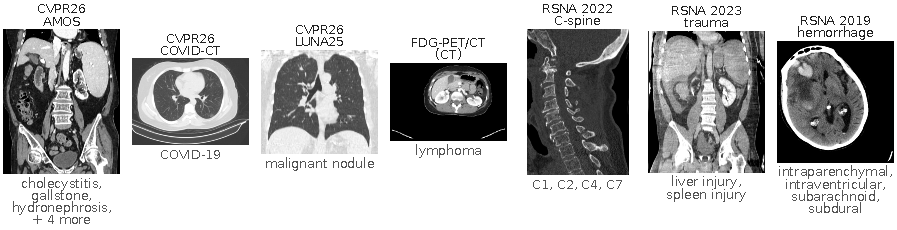
\includegraphics[width=\textwidth,height=0.74\textheight,keepaspectratio]{figures/fig_examples_cls.pdf}
\caption{One held-out case per classification source: the case with the most positive labels, listed below it. Views are fixed per source and pass through the body's center of mass: coronal for AMOS, LUNA25 and RSNA 2023, sagittal for the cervical spine, and axial for COVID-CTset (thick slices), FDG-PET/CT (whole body) and head CT. Windows are soft tissue, lung (COVID-CTset, LUNA25), bone (cervical spine) and brain (hemorrhage).}
\label{fig:examples}
\end{figure}

\clearpage
\section{Success and failure cases}
\label{app:cases}

\begin{figure}[H]
\centering
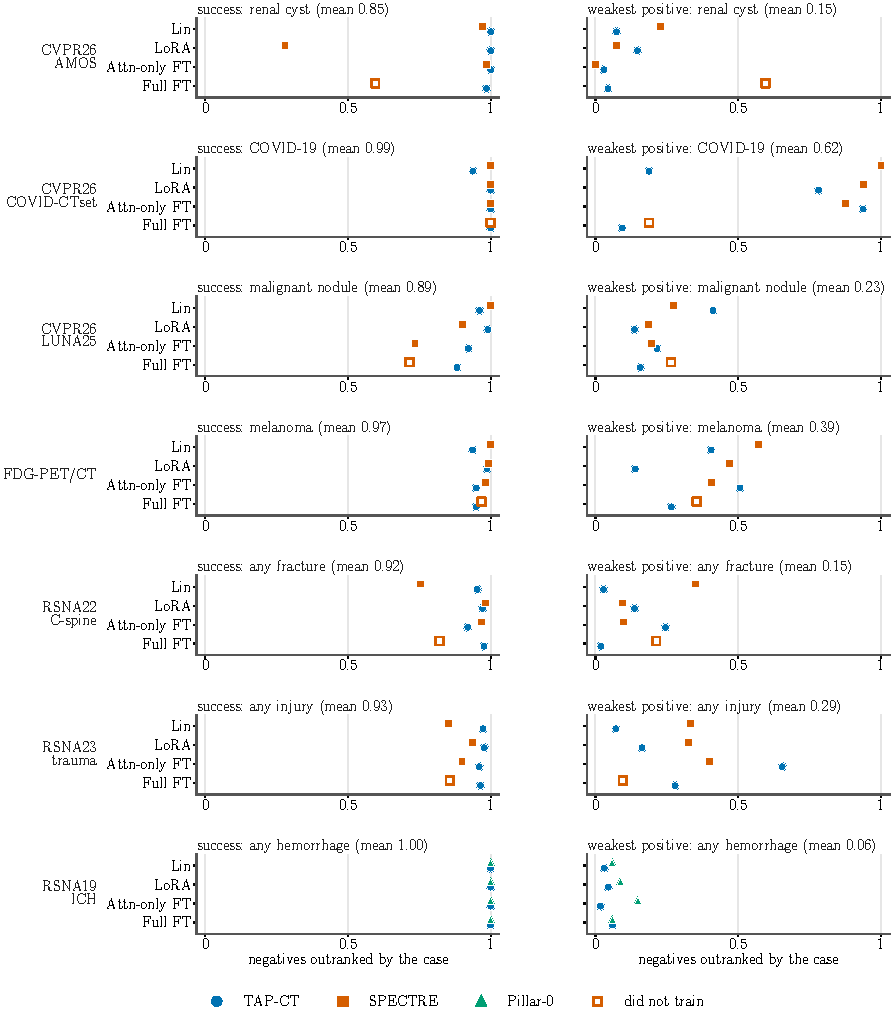
\includegraphics[width=\textwidth,height=0.74\textheight,keepaspectratio]{figures/fig_cases_cls.pdf}
\caption{Classification success (left) and failure (right) cases, one positive held-out case per source. Markers give the share of held-out negatives the case outranks for each method and backbone (1: ranked above every negative; dotted line: 0.5); the title gives the label and the case's mean over methods and backbones. Rows are the three CVPR26 sources, FDG-PET/CT, the RSNA 2022 cervical spine, RSNA 2023 trauma and RSNA 2019 hemorrhage.}
\label{fig:casescls}
\end{figure}

\begin{figure}[H]
\centering
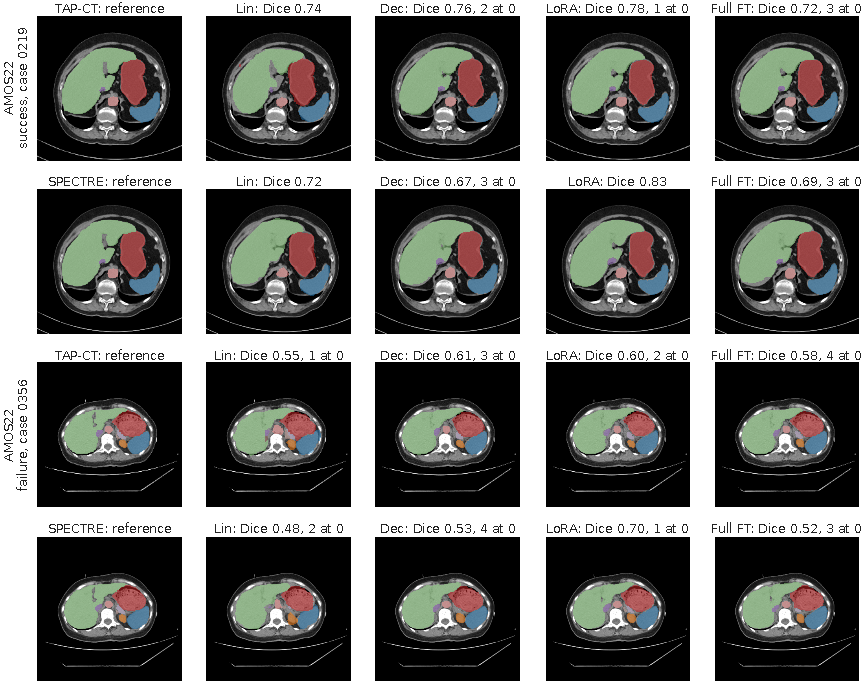
\includegraphics[width=0.9\textwidth,height=0.66\textheight,keepaspectratio]{figures/fig_cases_seg_amos22.pdf}
\caption{Segmentation success and failure cases on AMOS22 (15 structures), joint model. Rows: the success case (top two) and the failure case (bottom two), each on TAP-CT and SPECTRE; columns: the reference and the predictions of Lin, Dec, LoRA and Full FT on the axial slice with the most reference foreground, soft-tissue window, colors per structure. Panel titles give the method's Dice for the whole case, averaged over its structures, and how many of them score 0. These are the adrenal glands for most adapted methods and, for some, the esophagus or the gallbladder.}
\label{fig:casesseg_amos22}
\end{figure}

\begin{figure}[H]
\centering
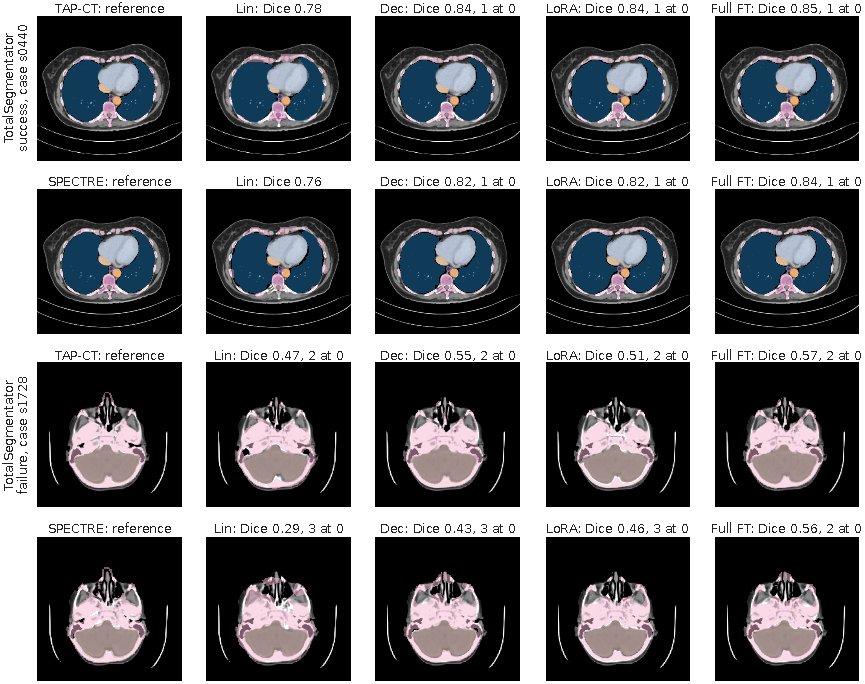
\includegraphics[width=0.9\textwidth,height=0.74\textheight,keepaspectratio]{figures/fig_cases_seg_totalseg.pdf}
\caption{As Figure~\ref{fig:casesseg_amos22}, for TotalSegmentator (15 merged structures). Every adapted joint model scores 0 on the merged glands in both cases; in the failure case some models also score 0 on the arteries, the liver, the lungs and airway or the gastrointestinal tract.}
\label{fig:casesseg_totalseg}
\end{figure}

\begin{figure}[H]
\centering
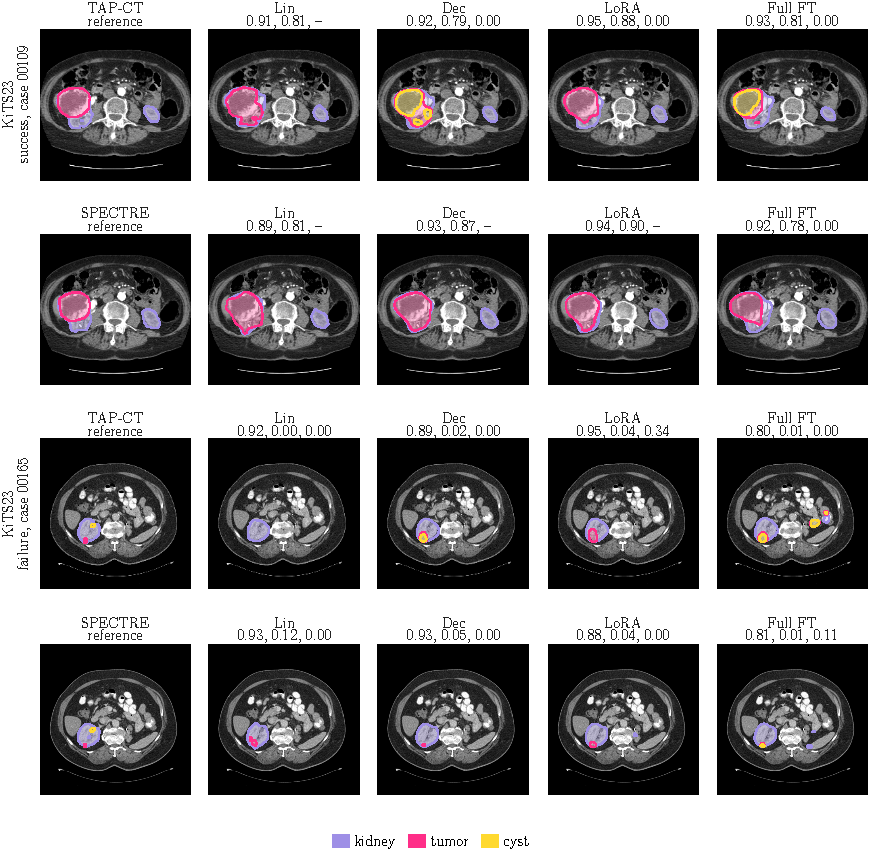
\includegraphics[width=0.9\textwidth,height=0.74\textheight,keepaspectratio]{figures/fig_cases_seg_kits23.pdf}
\caption{As Figure~\ref{fig:casesseg_amos22}, for KiTS23; panel titles give the Dice of each structure (kidney / tumor / cyst; \textendash: absent from both reference and prediction).}
\label{fig:casesseg_kits23}
\end{figure}

\begin{figure}[H]
\centering
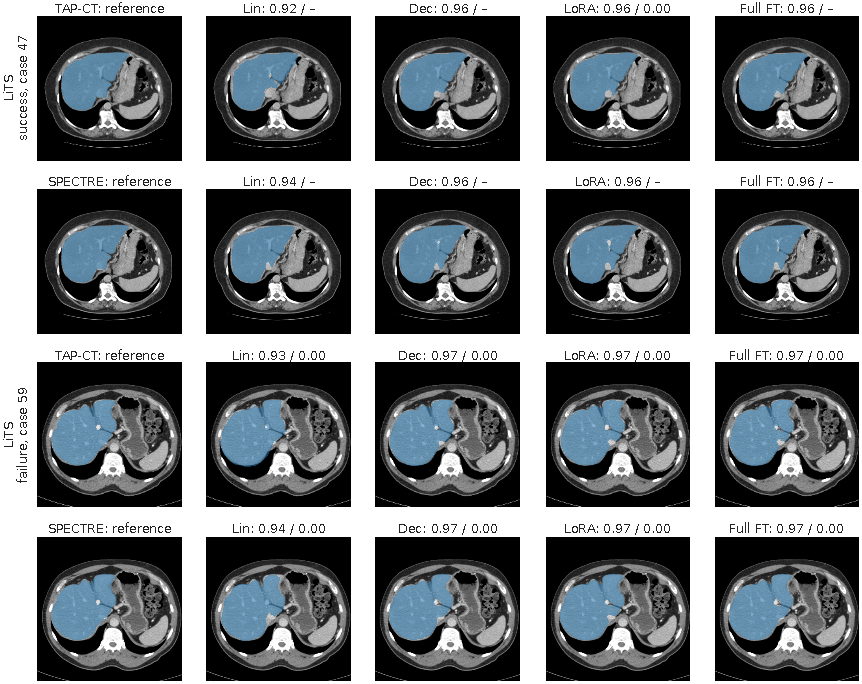
\includegraphics[width=0.9\textwidth,height=0.74\textheight,keepaspectratio]{figures/fig_cases_seg_lits.pdf}
\caption{As Figure~\ref{fig:casesseg_amos22}, for LiTS, except that panel titles give the Dice of each structure (liver / tumor; \textendash: absent from both reference and prediction). Neither case has a tumor in the reference, so a method's tumor Dice is undefined when it predicts no tumor and 0 when it predicts any: in the success case only LoRA on TAP-CT predicts a tumor somewhere in the volume, and in the failure case every method does, while all segment the liver well. The failure is therefore a false-positive tumor, which the per-structure Dice counts as 0, and not a missed one; the overlay shows the structure with the highest logit at each voxel, which hides the predicted tumor under the liver in all but one run.}
\label{fig:casesseg_lits}
\end{figure}

\begin{figure}[H]
\centering
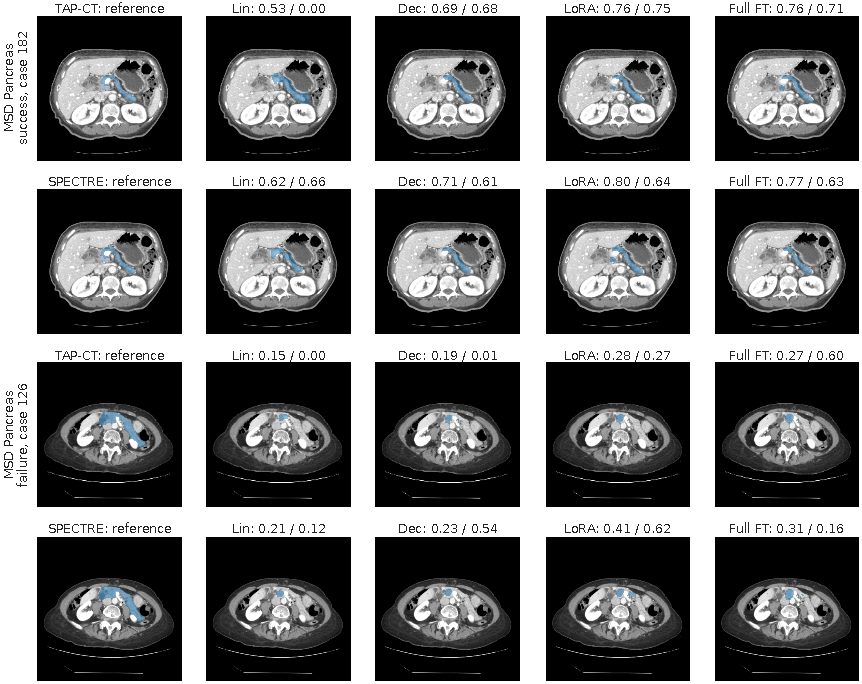
\includegraphics[width=0.9\textwidth,height=0.74\textheight,keepaspectratio]{figures/fig_cases_seg_msd_pancreas.pdf}
\caption{As Figure~\ref{fig:casesseg_amos22}, for MSD Pancreas; panel titles give the Dice of each structure (pancreas / tumor; \textendash: absent from both reference and prediction).}
\label{fig:casesseg_msd_pancreas}
\end{figure}


\end{document}
